%%%%%%%%%%%%%%%%%%%%%%%%%%%%%%%%%%%%%%%%%%%%%%%%%%%%%%%%%%%%%%%%%%
%%%%%%%%%%%%%%%%%%%%%%%%%%%%%%%%%%%%%%%%%%%%%%%%%%%%%%%%%%%%%%%%%%
\chapter{Diagramme erstellen}
\label{sec:graphics}
%%%%%%%%%%%%%%%%%%%%%%%%%%%%%%%%%%%%%%%%%%%%%%%%%%%%%%%%%%%%%%%%%%
%%%%%%%%%%%%%%%%%%%%%%%%%%%%%%%%%%%%%%%%%%%%%%%%%%%%%%%%%%%%%%%%%%

\index{Diagramm|see{Grafik}}
Daten lassen sich in R mit Hilfe einer Vielzahl von Diagrammtypen grafisch darstellen, wobei hier nur auf eine Auswahl der verfügbaren Typen eingegangen werden kann. Für eine umfassende Dokumentation vgl.\ \citeA{Murrell2005} und \citeA{Unwin2015}.\footnote{Viele Beispiele zeigt \url{https://www.r-graph-gallery.com/}} Während sich dieses Kapitel auf den Basisumfang von R konzentriert, geht Kap.\ \ref{sec:ggplot} auf das beliebte Zusatzpaket \lstinline!ggplot2! ein \cite{Wickham2009a}.

In R werden zwei Arten von Grafikfunktionen unterschieden: \emph{High-Level}-Funktionen\index{Grafik!High-Level-Funktion|textbf} erstellen eigenständig ein komplettes Diagramm inkl.\ Achsen, während \emph{Low-Level}-Funktionen\index{Grafik!Low-Level-Funktion|textbf} lediglich ein bestimmtes Element einem bestehenden Diagramm hinzufügen. Einen kurzen Überblick über die Gestaltungsmöglichkeiten vermittelt\index[func]{demo()@\lstinline{demo()}} \lstinline!demo(graphics)!.

%%%%%%%%%%%%%%%%%%%%%%%%%%%%%%%%%%%%%%%%%%%%%%%%%%%%%%%%%%%%%%%%%%
%%%%%%%%%%%%%%%%%%%%%%%%%%%%%%%%%%%%%%%%%%%%%%%%%%%%%%%%%%%%%%%%%%
\section{Grafik-Devices}
%%%%%%%%%%%%%%%%%%%%%%%%%%%%%%%%%%%%%%%%%%%%%%%%%%%%%%%%%%%%%%%%%%
%%%%%%%%%%%%%%%%%%%%%%%%%%%%%%%%%%%%%%%%%%%%%%%%%%%%%%%%%%%%%%%%%%

%%%%%%%%%%%%%%%%%%%%%%%%%%%%%%%%%%%%%%%%%%%%%%%%%%%%%%%%%%%%%%%%%%
%%%%%%%%%%%%%%%%%%%%%%%%%%%%%%%%%%%%%%%%%%%%%%%%%%%%%%%%%%%%%%%%%%
\subsection{Aufbau und Verwaltung von Grafik-Devices}
\label{sec:device}
%%%%%%%%%%%%%%%%%%%%%%%%%%%%%%%%%%%%%%%%%%%%%%%%%%%%%%%%%%%%%%%%%%
%%%%%%%%%%%%%%%%%%%%%%%%%%%%%%%%%%%%%%%%%%%%%%%%%%%%%%%%%%%%%%%%%%

\index{Grafik!device}
\index{Grafik!Ausgabe}
\index{Grafik!Ränder}
\index{Grafik!Regionen}
Die Ausgabe von Befehlen zum Erstellen einer Grafik kann in verschiedenen Ausgabekanälen, den\ \emph{devices} erfolgen. Ein device lässt sich wie eine leere Leinwand vorstellen, auf der mit Grafikfunktionen einzelne Inhalte wie mit einem Pinsel eingezeichnet werden. Die Fläche des device ist dabei in drei ineinander verschachtelte Regionen eingeteilt: die gesamte Device-Region mit den äußeren Rändern, die innerhalb dieser Ränder liegende \emph{Figure}-Region und die in diese eingebettete \emph{Plot}-Region, in die die Datenpunkte und andere Grafikelemente eingezeichnet werden (Abb.\ \ref{fig:margins}).\footnote{Weitere Details erklärt unter \url{https://www.rstudio.com/resources/cheatsheets/} das Dokument \emph{How big is your graph?}} In der Voreinstellung ist ein device ein separates Grafikfenster, es können aber etwa auch Dateien in verschiedenen Grafikformaten als device dienen.

\begin{figure}[ht]
\centering
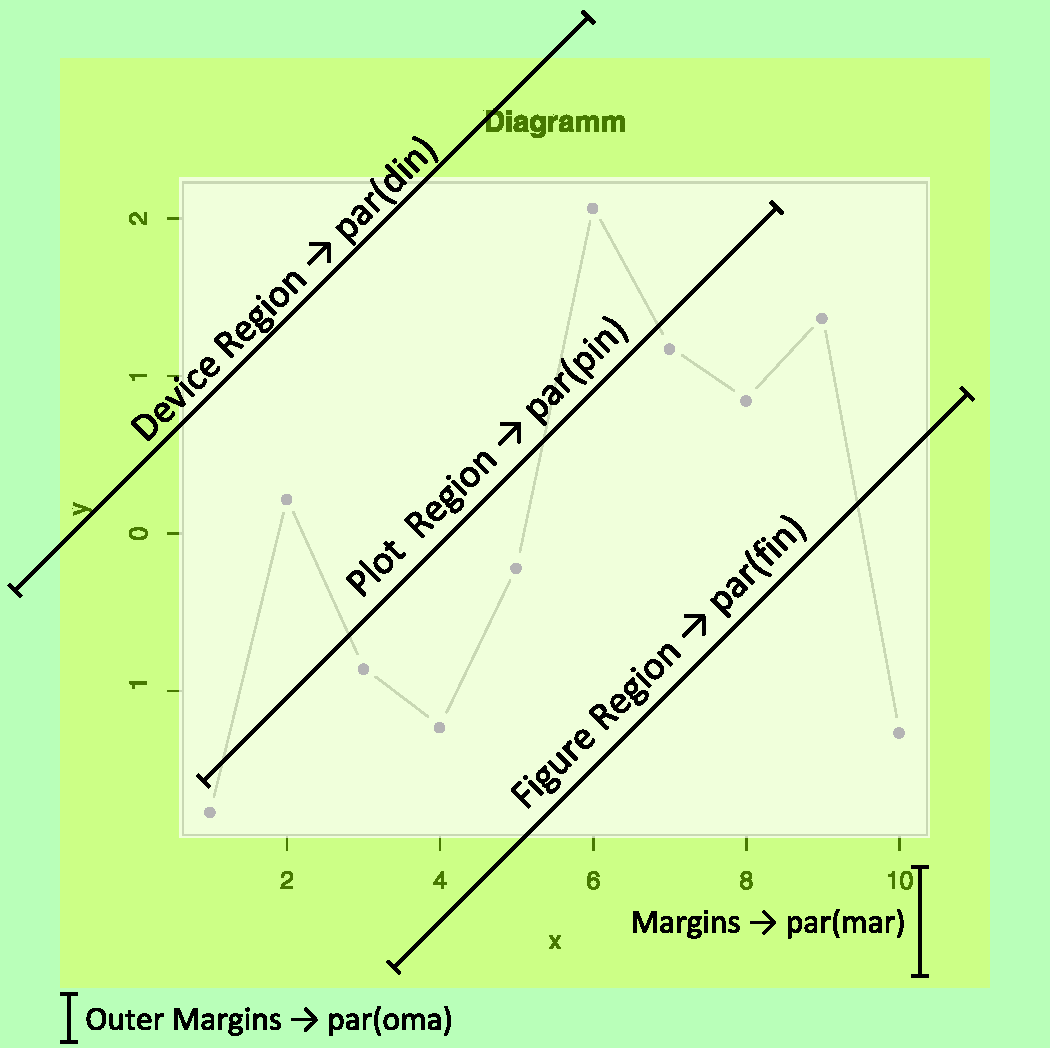
\includegraphics[width=8cm]{devMargins}
\vspace*{-0.5em}
\caption{Regionen und Ränder eines device samt Möglichkeiten, ihre Größe mit \lstinline!par()! ausgeben und ggf.\ verändern zu können (Abschn.\ \ref{sec:par})}
\label{fig:margins}
\end{figure}

\index{Grafik!Fenster öffnen}
\index{Grafik!device!verwalten}
Sofern noch kein Grafikfenster existiert, öffnet es sich mit Eingabe des ersten\index{Grafik!High-Level-Funktion} High-Level-Grafikbefehls automatisch -- in RStudio im \emph{Plots} Tab. In dieses Fenster werden dann alle weiteren Ausgaben grafischer Funktionen hinein gezeichnet, wobei im Fall von High-Level-Funktionen ein ggf.\ bereits vorhandener Inhalt gelöscht wird. Soll für die Ausgabe einer Grafikfunktion zusätzlich zu bereits bestehenden ein neues, zunächst leeres Fenster geöffnet werden, geschieht dies unter Windows mit\index[func]{windows()@\lstinline{windows()}}
\begin{lstlisting}
windows(width=<<Breite>>, height=<<Höhe>>)
\end{lstlisting}

Unter MacOS ist\index[func]{quartz()@\lstinline{quartz()}} \lstinline!quartz()! und unter Unix/Linux\index[func]{x11()@\lstinline{x11()}} \lstinline!x11()! der äquivalente Befehl. Unabhängig vom Betriebssystem erzielt \index[func]{dev.new()@\lstinline{dev.new()}} \lstinline!dev.new()! in der Voreinstellung denselben Effekt. Breite und Höhe des Fensters können über die Argumente \lstinline!width! und \lstinline!height! in der Einheit inch bestimmt werden. Bei mehreren geöffneten devices sind alle bis auf eines inaktiv, das im Fenstertitel die Bezeichnung \emph{(ACTIVE)} trägt. Die Bezeichnung bedeutet, dass in dieses device die Ausgabe der folgenden Grafikfunktion gezeichnet wird, während die Inhalte der anderen devices unverändert bleiben. Um sich einen Überblick über alle aktuell geöffneten devices zu verschaffen, dient der Befehl\index[func]{dev.list()@\lstinline{dev.list()}} \lstinline!dev.list()!.
\begin{lstlisting}
> dev.new(); dev.new(); dev.new()
> dev.list()
windows  windows  windows
      2        3        4
\end{lstlisting}

Die Ausgabe zeigt, welche Ausgabekanäle offen sind. Jedes device besitzt dafür eine laufende Nummer, wobei das erste device die $2$ erhält. Um zu erfahren, welcher der Ausgabekanäle aktiv ist, dient\index[func]{dev.cur()@\lstinline{dev.cur()}} \lstinline!dev.cur()! (\emph{device current}).
\begin{lstlisting}
> dev.cur()
windows
      4
\end{lstlisting}

\index{Grafik!device!verwalten}
Die Ausgabe besteht in der fortlaufenden Nummer des aktiven device. \lstinline!dev.prev()!\index[func]{dev.prev()@\lstinline{dev.prev()}} (\emph{device previous}) und\index[func]{dev.next()@\lstinline{dev.next()}} \lstinline!dev.next()! geben bei mehreren geöffneten devices die Nummer desjenigen device zurück, das sich unmittelbar vor bzw.\ unmittelbar hinter dem aktiven device befindet. Diese Information kann etwa zum Wechseln des aktiven device mit\index[func]{dev.set()@\lstinline{dev.set()}} \lstinline!dev.set(<<Nummer>>)! verwendet werden, damit die Ausgabe der folgenden Grafikfunktionen dort erfolgt.
\begin{lstlisting}
> dev.set(3)                            # aktiviere device 3
windows
      3

> dev.set(dev.next())                   # aktiviere das folgende device
windows
      4
\end{lstlisting}

\index{Grafik!device!verwalten}
Das aktive device wird mit\index[func]{dev.off()@\lstinline{dev.off()}} \lstinline!dev.off()! geschlossen. Handelt es sich um ein Grafikfenster, hat dies denselben Effekt, wie das Fenster per Mausklick zu schließen. Die Ausgabe von \lstinline!dev.off()! gibt an, welches fortan das aktive device ist. Ohne weitere geöffnete devices ist dies das \emph{NULL}-device mit der Nummer $1$. Alle offenen devices lassen sich gleichzeitig mit \lstinline!graphics.off()!\index[func]{graphics.off()@\lstinline{graphics.off()}} schließen.
\begin{lstlisting}
> dev.off()                             # aktuelles device schließen
windows
      2

> graphics.off()                        # alle devices schließen
\end{lstlisting}

%%%%%%%%%%%%%%%%%%%%%%%%%%%%%%%%%%%%%%%%%%%%%%%%%%%%%%%%%%%%%%%%%%
%%%%%%%%%%%%%%%%%%%%%%%%%%%%%%%%%%%%%%%%%%%%%%%%%%%%%%%%%%%%%%%%%%
\subsection{Grafiken speichern}
\label{sec:saveDiag}
%%%%%%%%%%%%%%%%%%%%%%%%%%%%%%%%%%%%%%%%%%%%%%%%%%%%%%%%%%%%%%%%%%
%%%%%%%%%%%%%%%%%%%%%%%%%%%%%%%%%%%%%%%%%%%%%%%%%%%%%%%%%%%%%%%%%%

\index{Grafik!speichern}
Alles, was sich in einem Grafikfenster anzeigen lässt, kann auch als Datei gespeichert werden -- in RStudio im \emph{Plots}-Tab mit dem Eintrag \emph{Export}. Ist ein Grafikfenster aktiviert, so ändert sich das Menü der R-Umgebung dahingehend, dass über \emph{Datei: Speichern als:} die Grafik in vielen Formaten gespeichert werden kann. Als Alternative erlaubt ein sich durch Rechtsklick auf das Grafikfenster öffnendes Kontextmenü, die Grafik in wenigen Formaten zu speichern. Dasselbe Kontextmenü enthält auch Einträge, um die Grafik in einem bestimmten Format in die Zwischenablage zu kopieren und so direkt anderen Programmen verfügbar zu machen.

Grafiken lassen sich auch befehlsgesteuert ohne den Umweg eines Grafikfensters in Dateien speichern. Unabhängig davon, in welchem Format dies geschehen soll, sind dafür drei Arbeitsschritte notwendig: Zunächst muss die Datei als Ausgabekanal (also als aktives device) festgelegt werden. Dazu dient etwa\index[func]{pdf()@\lstinline{pdf()}} \lstinline!pdf()!, wenn die Grafik im PDF-Format zu speichern ist. Es folgen Befehle zum Erstellen von Diagrammen oder Einfügen von Grafikelementen, deren Ausgabe dann nicht auf dem Bildschirm erscheint, sondern direkt in die Datei umgeleitet wird. Schließlich ist der Befehl \lstinline!dev.off()! oder \lstinline!graphics.off()! notwendig, um die Ausgabe in die Datei zu beenden und das device zu schließen.

\index{Grafik!Formate}
Als Dateiformate stehen viele der üblichen bereit, vgl.\ \lstinline!?device! für eine Aufstellung. Beispielhaft seien hier \lstinline!pdf()! und \lstinline!jpeg()! \index[func]{jpeg()@\lstinline{jpeg()}} betrachtet.\footnote{Alternativ stellt das Paket\index[pack]{Cairo@\lstinline{Cairo}} \lstinline!Cairo! \cite{Urbanek2014} die gleichnamige Funktion\index[func]{Cairo()@\lstinline{Cairo()}} zur Verfügung, mit der Diagramme in vielen Dateiformaten auch in hoher Auflösung und mit automatischer Kantenglättung gespeichert werden können.}
\begin{lstlisting}
pdf(file="<<Dateiname>>", width=<<Breite>>, height=<<Höhe>>)
jpeg(filename="<<Dateiname>>", width=<<Breite>>, height=<<Höhe>>,
     units="px", quality=<<Bildqualität>>)
\end{lstlisting}

Unter \lstinline!file! bzw.\ \lstinline!filename! ist der Name der Ausgabedatei einzutragen -- ggf.\ inkl.\ einer Pfadangabe (Abschn.\ \ref{sec:files}). Sollen mehrere Grafiken mit gleichem Namensschema unter Zuhilfenahme einer fortlaufenden Nummer erzeugt werden, ist ein spezielles Namensformat zu verwenden, das in der Hilfe erläutert wird. Mit \lstinline!width! und \lstinline!height! wird die Größe der Grafik kontrolliert. Beide Angaben sind bei \lstinline!pdf()! in der Einheit inch zu tätigen, während bei \lstinline!jpeg()! über das Argument \lstinline!units! festgelegt werden kann, auf welche Maßeinheit sie sich beziehen. Voreinstellung ist die Anzahl der pixel, als Alternativen stehen \lstinline!in! (inch), \lstinline!cm! und \lstinline!mm! zur Auswahl. Schließlich kann bei Bildern im JPEG-Format festgelegt werden, wie stark die Daten komprimiert werden sollen, wobei die Kompression mit einem Verlust an Bildinformationen verbunden ist. Das Argument \lstinline!quality! erwartet einen sich auf die höchstmögliche Bildqualität beziehenden Prozentwert -- ein kleinerer Wert bedeutet hier eine geringere Bildqualität, die dann stärkere Kompression führt dafür aber auch zu einer geringeren Dateigröße.

Hier soll demonstriert werden, wie eine einfache Grafik im PDF-Format gespeichert wird.
\begin{lstlisting}
> pdf("pdf_test.pdf")                  # device öffnen (mit Dateinamen)
> plot(1:10, rnorm(10))                # Grafik einzeichnen
> dev.off()                            # device schließen
\end{lstlisting}

%\index{Grafik!kopieren}
%Die Inhalte eines aktiven device können durch\index[func]{dev.copy()@\lstinline{dev.copy()}} \lstinline!dev.copy()! in ein neues device kopiert werden. Dabei ist entweder die Nummer des bereits geöffneten Ziel-Device zu nennen oder anzugeben, welche Art von device mit den bestehenden Inhalten neu geöffnet werden soll.
%\begin{lstlisting}
%> dev.copy(device=<<Device-Typ>>, ..., which=<<Device-Nummer>>)
%\end{lstlisting}
%
%Ist das Ziel-Device noch nicht geöffnet, findet das \lstinline!device! Argument Verwendung, das (ohne Anführungszeichen) den Namen einer Funktion erwartet, mit der ein device eines bestimmten Typs geöffnet werden kann, etwa \lstinline!pdf!. Andernfalls gibt \lstinline!which! die Nummer des geöffneten Ziel-Device an. Benötigt das neu zu erstellende device seinerseits Argumente -- etwa Dateinamen oder Angaben zur Größe der Grafik, so können diese anstelle der \lstinline!...! durch Komma getrennt genannt werden.
%\begin{lstlisting}
%> plot(1:10, rnorm(10))                # Grafikfenster + Diagramm öffnen
%
%# Inhalt des Fensters in JPEG-Bild speichern,
%# dabei Dateinamen und Kompressionsgrad angeben
%> dev.copy(jpeg, filename="copied.jpg", quality=90)
%> graphics.off()                       # beide offenen devices schließen
%\end{lstlisting}

%%%%%%%%%%%%%%%%%%%%%%%%%%%%%%%%%%%%%%%%%%%%%%%%%%%%%%%%%%%%%%%%%%
%%%%%%%%%%%%%%%%%%%%%%%%%%%%%%%%%%%%%%%%%%%%%%%%%%%%%%%%%%%%%%%%%%
\section{Streu- und Liniendiagramme}
\label{sec:plot}
%%%%%%%%%%%%%%%%%%%%%%%%%%%%%%%%%%%%%%%%%%%%%%%%%%%%%%%%%%%%%%%%%%
%%%%%%%%%%%%%%%%%%%%%%%%%%%%%%%%%%%%%%%%%%%%%%%%%%%%%%%%%%%%%%%%%%

\index{Grafik!Streudiagramm}
In zweidimensionalen Streudiagrammen (\emph{scatterplots}) werden mit \lstinline!plot()! Wertepaare in Form von Punkten in einem kartesischen Koordinatensystem dargestellt, wobei ein Wert die Position des Punkts entlang der Abszisse ($x$-Achse) und der andere Wert die Position des Punkts entlang der Ordinate ($y$-Achse) bestimmt. Die Punkte können dabei für ein Liniendiagramm durch Linien verbunden oder für ein Streudiagramm als Punktwolke belassen werden.

%%%%%%%%%%%%%%%%%%%%%%%%%%%%%%%%%%%%%%%%%%%%%%%%%%%%%%%%%%%%%%%%%%
%%%%%%%%%%%%%%%%%%%%%%%%%%%%%%%%%%%%%%%%%%%%%%%%%%%%%%%%%%%%%%%%%%
\subsection{Streudiagramme mit \texttt{plot()}}
%%%%%%%%%%%%%%%%%%%%%%%%%%%%%%%%%%%%%%%%%%%%%%%%%%%%%%%%%%%%%%%%%%
%%%%%%%%%%%%%%%%%%%%%%%%%%%%%%%%%%%%%%%%%%%%%%%%%%%%%%%%%%%%%%%%%%

\index[func]{plot()@\lstinline{plot()}|textbf}
\index{Grafik!Liniendiagramm}
\begin{lstlisting}
plot(x=<<Vektor>>, y=<<Vektor>>, type="<<Option>>", main="<<Diagrammtitel>>",
     sub="<<Untertitel>>", asp=<<Seitenverhältnis Höhe/Breite>>)
\end{lstlisting}

Unter \lstinline!x! und \lstinline!y! sind die $x$- bzw.\ $y$-Koordinaten der Punkte jeweils als Vektor einzutragen. Wird nur ein Vektor angegeben, werden seine Werte als $y$-Koordinaten interpretiert und die $x$-Koordinaten durch die Indizes des Vektors gebildet.\footnote{Dagegen erzeugt \lstinline!plot(<<Faktor>>, ...)! ein Säulendiagramm der Häufigkeiten jeder Faktorstufe (Abschn.\ \ref{sec:barplot}), da \lstinline!plot()! eine generische Funktion ist (Abschn.\ \ref{sec:funcGeneric}).} Das Argument \lstinline!type! hat mehrere mögliche Ausprägungen, die das Aussehen der Datenmarkierungen im Diagramm bestimmen (Tab.\ \ref{tab:plotArgs}, Abb.\ \ref{fig:plotTypes}). Der Diagrammtitel kann als Zeichenkette für \lstinline!main! angegeben werden, der Untertitel für \lstinline!sub!. Das Verhältnis von Höhe zu Breite jeweils einer Skaleneinheit im Diagramm kontrolliert das Argument \lstinline!asp! (\emph{aspect ratio}), für weitere Argumente vgl.\ \lstinline!?plot.default!.

Die Koordinaten der Punkte können auch über andere Wege angegeben werden: Als Modellformel lautet der Aufruf \lstinline!plot(<<y-Koord.>> ~ <<x-Koord.>>, data=<<Datensatz>>)!.\footnote{Hat die Modellformel die Form \lstinline!<<y-Koord.>> ~ <<Faktor>>!, werden in einem Diagramm getrennt für die von \lstinline!<<Faktor>>! definierten Gruppen boxplots dargestellt (Abschn.\ \ref{sec:boxplot}).} Wenn die in der Modellformel verwendeten Variablen aus einem Datensatz stammen, ist dieser unter \lstinline!data! zu nennen. Weiter ist es möglich, eine Liste mit zwei Komponenten \lstinline!x! und \lstinline!y! anzugeben, die die Koordinaten enthalten. Schließlich kann einfach eine Matrix mit zwei Spalten für die $(x, y)$-Koordinaten übergeben werden.

%\begin{longtable}{p{2.3cm}p{9.5cm}}
\begin{table}[ht]
\centering
\caption{Mögliche Werte für das Argument \lstinline!type! von \lstinline!plot()!}
\label{tab:plotArgs}
\begin{tabular}{p{2.3cm}p{10.2cm}}
\hline
\sffamily Wert für \lstinline!type! & \sffamily Bedeutung\\\hline\hline
\lstinline!"p"! & Punkte\\
\lstinline!"l"! & durchgehende Linien. Durch eng gesetzte Stützstellen können Funktionskurven beliebiger Form approximiert werden\\
\lstinline!"b"! & Punkte und Linien\\
\lstinline!"c"! & unterbrochene Linien\\
\lstinline!"o"! & Punkte und Linien, aber überlappend\\
\lstinline!"h"! & senkrechte Linien zu jedem Datenpunkt (\emph{spike plot})\\
\lstinline!"s"! & Stufendiagramm\\
\lstinline!"S"! & Stufendiagramm mit anderer Reihenfolge von vertikalen und horizontalen Schritten zur nächsten Stufe\\
\lstinline!"n"! & fügt dem Diagramm keine Datenpunkte hinzu (\emph{no plotting})\\\hline
\end{tabular}
\end{table}
%\end{longtable}

\begin{lstlisting}
> vec <- rnorm(10)                            # Daten

# das Argument xlab=NA entfernt die Bezeichnung der x-Achse
> plot(vec, type="p", xlab=NA, main="type p")
> plot(vec, type="l", xlab=NA, main="type l")
> plot(vec, type="b", xlab=NA, main="type b")
> plot(vec, type="o", xlab=NA, main="type o")
> plot(vec, type="s", xlab=NA, main="type s")
> plot(vec, type="h", xlab=NA, main="type h")
\end{lstlisting}

\begin{figure}[ht]
\centering
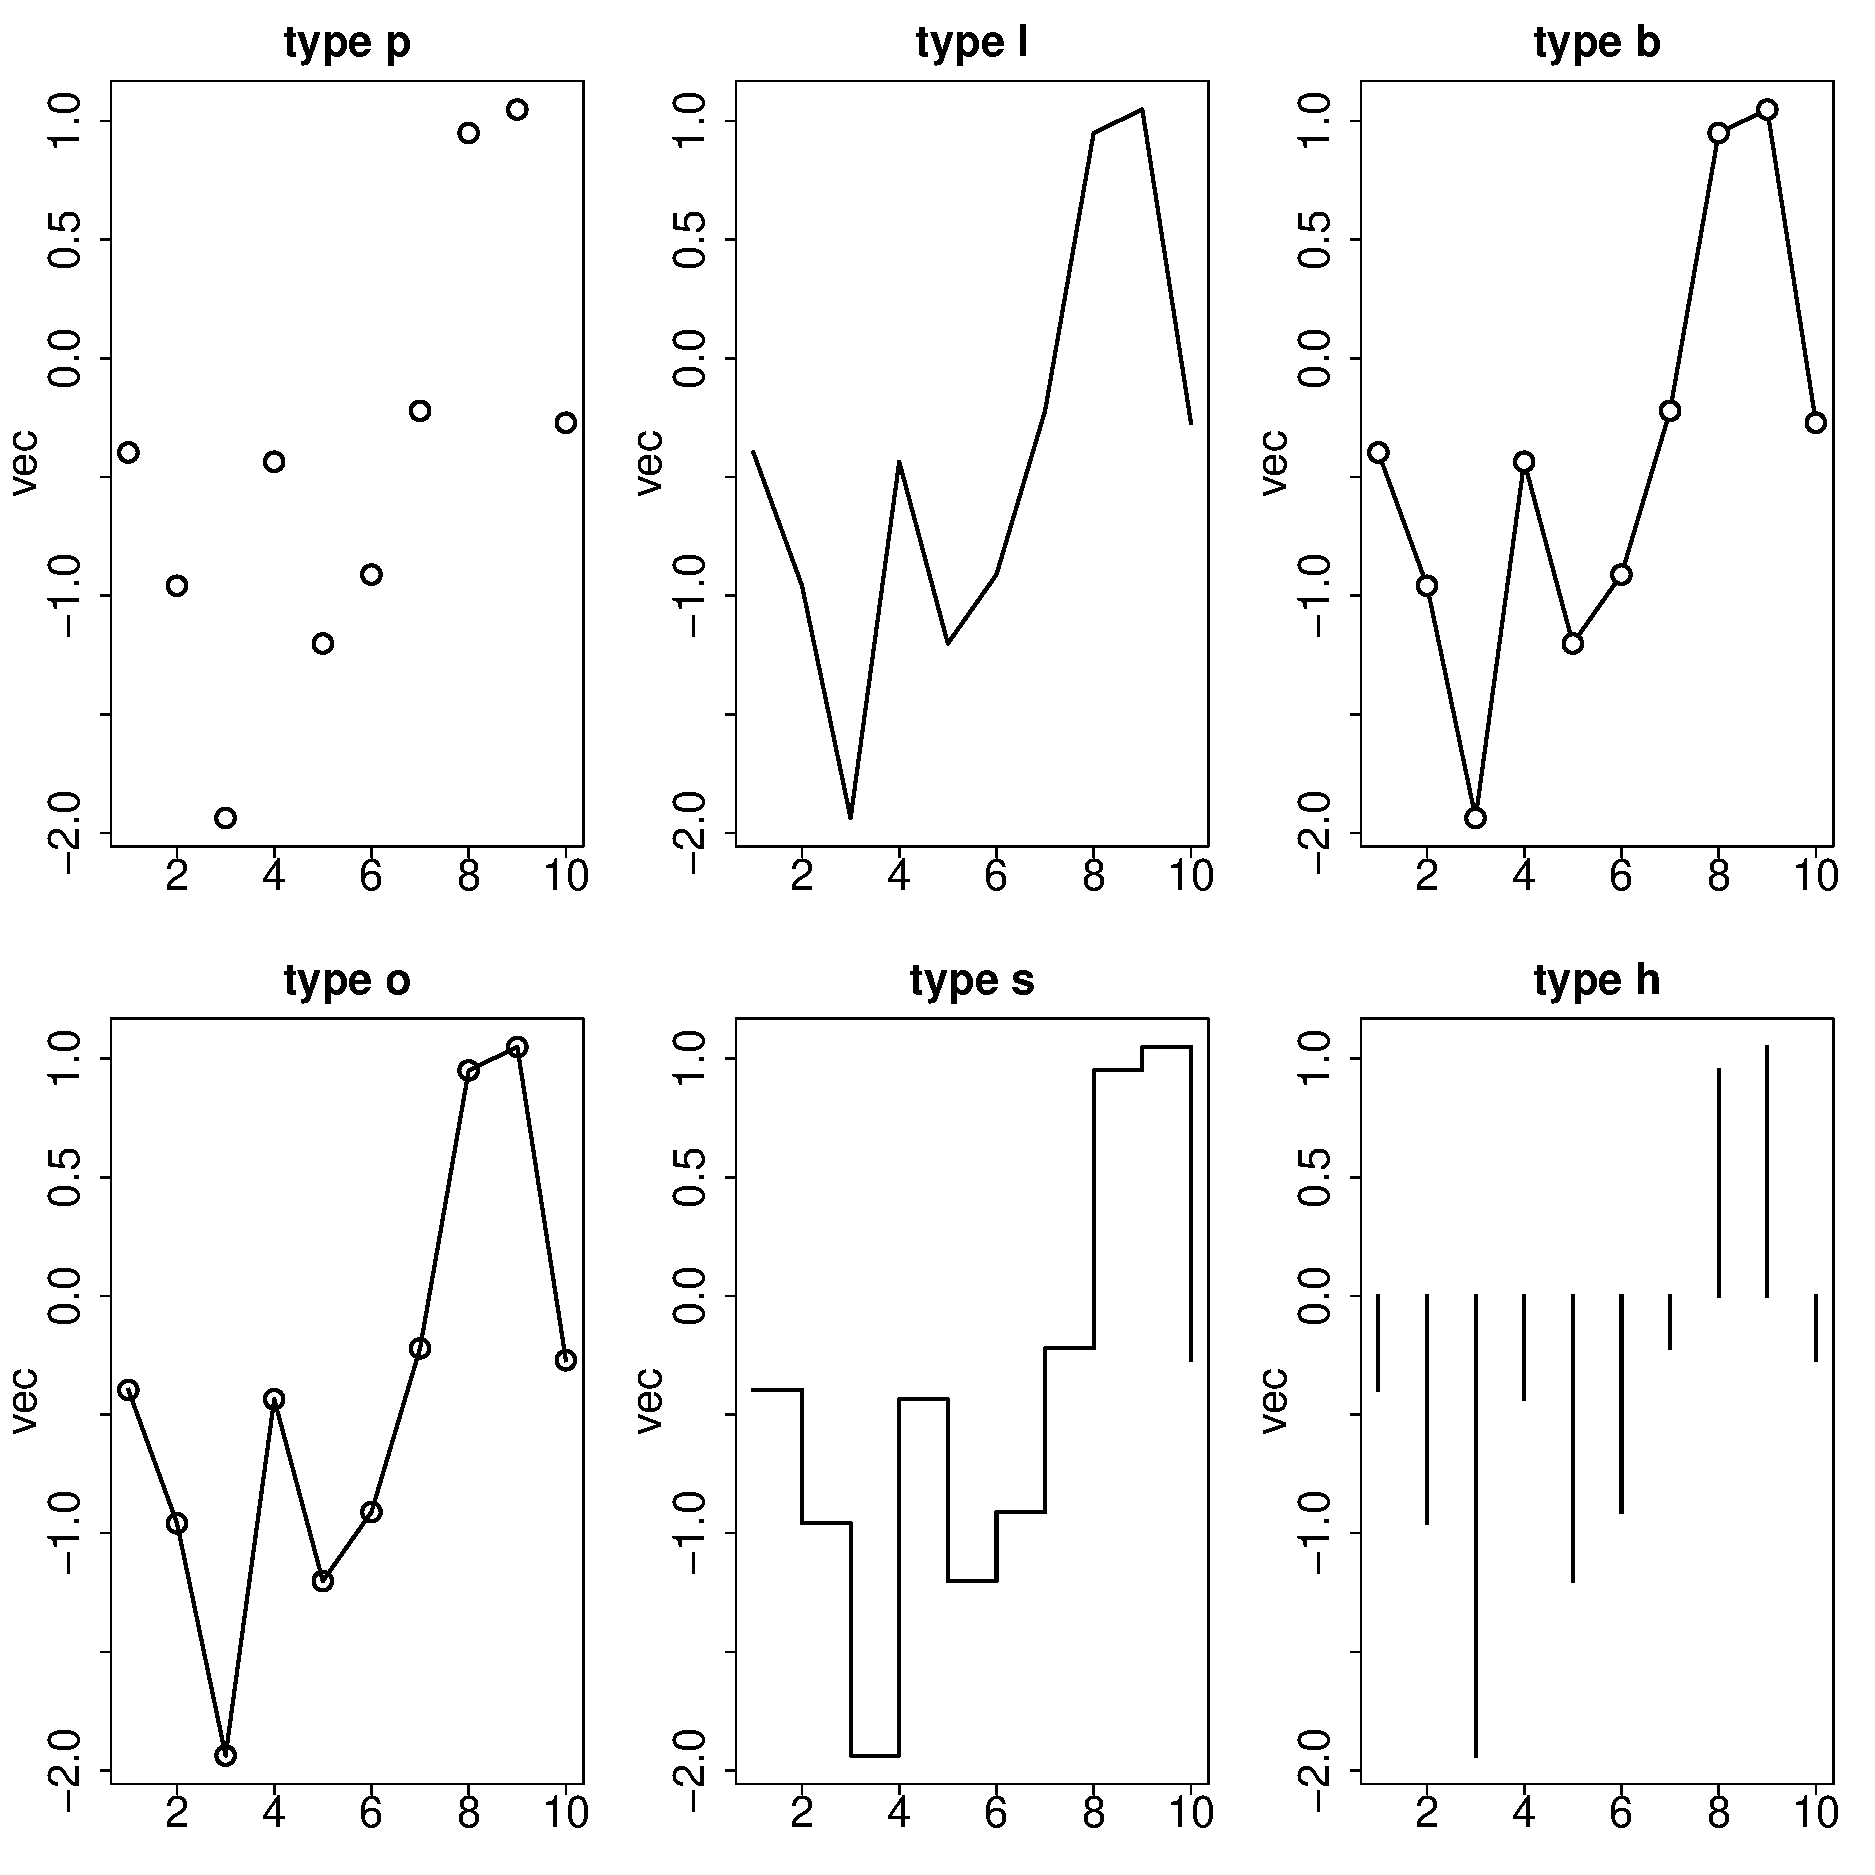
\includegraphics[width=12.5cm]{plotTypes}
\vspace*{-1em}
\caption{Mit \lstinline!plot(type="<<Option>>")! erzeugbare Diagrammarten}
\label{fig:plotTypes}
\end{figure}

%%%%%%%%%%%%%%%%%%%%%%%%%%%%%%%%%%%%%%%%%%%%%%%%%%%%%%%%%%%%%%%%%%
%%%%%%%%%%%%%%%%%%%%%%%%%%%%%%%%%%%%%%%%%%%%%%%%%%%%%%%%%%%%%%%%%%
\subsection{Datenpunkte eines Streudiagramms identifizieren}
%%%%%%%%%%%%%%%%%%%%%%%%%%%%%%%%%%%%%%%%%%%%%%%%%%%%%%%%%%%%%%%%%%
%%%%%%%%%%%%%%%%%%%%%%%%%%%%%%%%%%%%%%%%%%%%%%%%%%%%%%%%%%%%%%%%%%

\index{Grafik!Datenpunkte identifizieren}
Werden viele Daten in einem Streudiagramm dargestellt, ist häufig nicht ersichtlich, zu welchem Wert ein bestimmter Datenpunkt gehört. Diese Information kann jedoch interessant sein, wenn etwa erst die grafische Betrachtung eines Datensatzes Besonderheiten der Verteilung verrät und die für bestimmte Datenpunkte verantwortlichen Untersuchungseinheiten identifiziert werden sollen. \lstinline!identify()!\index[func]{identify()@\lstinline{identify()}} erlaubt es, Werte in einem Streudiagramm interaktiv zu identifizieren.
\begin{lstlisting}
identify(x=<<x-Koordinaten>>, y=<<y-Koordinaten>>)
\end{lstlisting}

Für \lstinline!x! und \lstinline!y! sollten dieselben Daten in Form von Vektoren mit $x$- und $y$-Koordinaten übergeben werden, die zuvor in einem noch geöffneten Grafikfenster als Streudiagramm dargestellt wurden. Wird nur ein Vektor angegeben, werden seine Werte als $y$-Koordinaten interpretiert und die $x$-Koordinaten durch die Indizes des Vektors gebildet. Durch Ausführen von \lstinline!identify()! ändert sich der Mauszeiger über der Diagrammfläche zu einem Kreuz. Mit einem Klick der linken Maustaste wird derjenige Datenpunkt identifiziert, der der Mausposition am nächsten liegt und sein Index dem Diagramm neben dem Datenpunkt hinzugefügt. Die Konsole ist in dieser Zeit blockiert. Der Vorgang kann mehrfach wiederholt und schließlich durch Klicken der rechten Maustaste über ein Kontextmenü beendet werden, woraufhin \lstinline!identify()! die Indizes der ausgemachten Punkte zurückgibt. In RStudio wird der Vorgang durch Drücken der \lstinline[language=]!ESC! Taste beendet.
\begin{lstlisting}
> vec <- rnorm(10)
> plot(vec)
> identify(vec)
# Mausclicks ...
[1] 1 4 5 8
\end{lstlisting}

%%%%%%%%%%%%%%%%%%%%%%%%%%%%%%%%%%%%%%%%%%%%%%%%%%%%%%%%%%%%%%%%%%
%%%%%%%%%%%%%%%%%%%%%%%%%%%%%%%%%%%%%%%%%%%%%%%%%%%%%%%%%%%%%%%%%%
\subsection{Streudiagramme mit \texttt{matplot()}}
%%%%%%%%%%%%%%%%%%%%%%%%%%%%%%%%%%%%%%%%%%%%%%%%%%%%%%%%%%%%%%%%%%
%%%%%%%%%%%%%%%%%%%%%%%%%%%%%%%%%%%%%%%%%%%%%%%%%%%%%%%%%%%%%%%%%%

\index{Grafik!Streudiagramm}
\index{Grafik!Liniendiagramm}
\index{Streudiagramm|see{Grafik}}
So wie durch \lstinline!plot()! ein Streudiagramm einer einzelnen Datenreihe erstellt wird, erzeugt \lstinline!matplot()! ein Streudiagramm für mehrere Datenreihen gleichzeitig\index[func]{matplot()@\lstinline{matplot()}} (Abb.\ \ref{fig:matplot}).
\begin{lstlisting}
matplot(x=<<Matrix>>, y=<<Matrix>>, type="<<Option>>", pch="<<Symbol>>")
\end{lstlisting}

Die Argumente sind dieselben wie für \lstinline!plot()!, lediglich $x$- und $y$-Koordinaten können nun als Matrizen an \lstinline!x! und \lstinline!y! übergeben werden. Dabei wird jede ihrer Spalten als eine separate Datenreihe interpretiert. Haben dabei alle Datenreihen dieselben $x$-Koordinaten, kann \lstinline!x! auch ein Vektor sein. Wird nur eine Matrix mit Koordinaten angegeben, werden diese als $y$-Koordinaten gedeutet und die $x$-Koordinaten durch die Zeilenindizes der Werte gebildet. In der Voreinstellung werden die Datenreihen in unterschiedlichen Farben dargestellt. Als Symbol für jeden Datenpunkt dienen die Ziffern 1--9, die mit der zur Datenreihe gehörenden Spaltennummer korrespondieren. Mit dem Argument \lstinline!pch! können auch andere Symbole Verwendung finden (Abschn.\ \ref{sec:par}, Abb. \ref{fig:pchLty}).
\begin{lstlisting}
> vec <- seq(from=-2*pi, to=2*pi, length.out=50)
> mat <- cbind(2*sin(vec), sin(vec-(pi/4)), 0.5*sin(vec-(pi/2)))
> matplot(vec, mat, type="b", xlab=NA, ylab=NA, pch=1:3,
+         main="Sinuskurven")
\end{lstlisting}

\begin{figure}[ht]
\centering
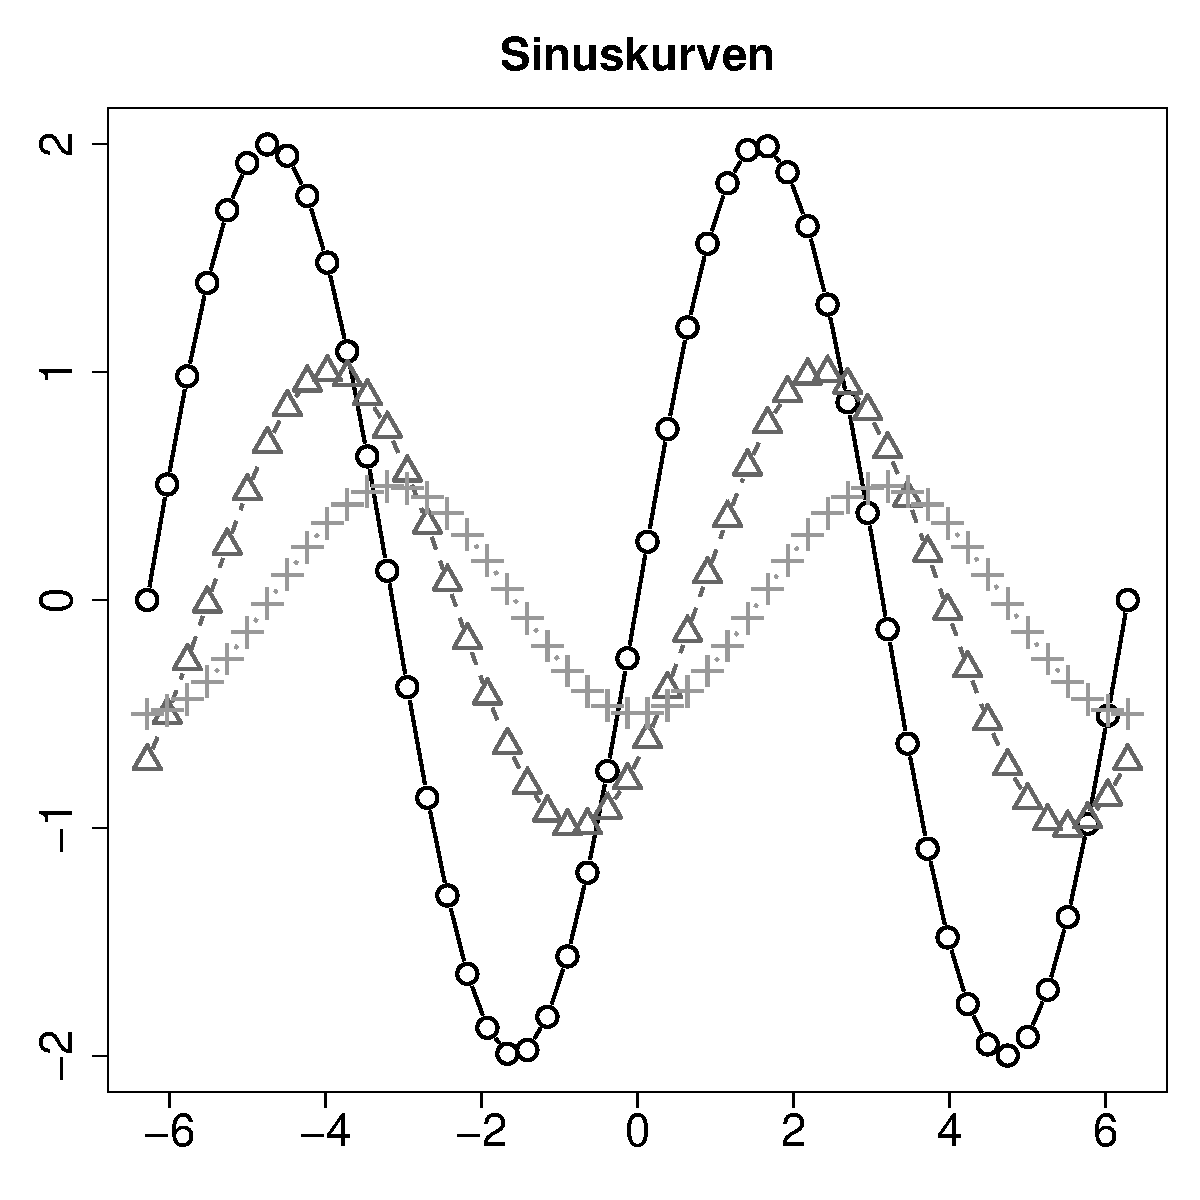
\includegraphics[width=8cm]{matplot}
\vspace*{-1.5em}
\caption{Mit \lstinline!matplot()! erzeugtes Streudiagramm}
\label{fig:matplot}
\end{figure}

%%%%%%%%%%%%%%%%%%%%%%%%%%%%%%%%%%%%%%%%%%%%%%%%%%%%%%%%%%%%%%%%%%
%%%%%%%%%%%%%%%%%%%%%%%%%%%%%%%%%%%%%%%%%%%%%%%%%%%%%%%%%%%%%%%%%%
\section{Diagramme formatieren}
\label{sec:graphFormat}
%%%%%%%%%%%%%%%%%%%%%%%%%%%%%%%%%%%%%%%%%%%%%%%%%%%%%%%%%%%%%%%%%%
%%%%%%%%%%%%%%%%%%%%%%%%%%%%%%%%%%%%%%%%%%%%%%%%%%%%%%%%%%%%%%%%%%

\lstinline!plot()! akzeptiert wie auch andere High-Level-Grafikfunktionen eine Vielzahl weiterer Argumente, mit denen ein Diagramm flexibel angepasst werden kann. Einige der wichtigsten Möglichkeiten zur individuellen Gestaltung werden im Folgenden vorgestellt.

%%%%%%%%%%%%%%%%%%%%%%%%%%%%%%%%%%%%%%%%%%%%%%%%%%%%%%%%%%%%%%%%%%
%%%%%%%%%%%%%%%%%%%%%%%%%%%%%%%%%%%%%%%%%%%%%%%%%%%%%%%%%%%%%%%%%%
\subsection{Grafikelemente formatieren}
\label{sec:par}
%%%%%%%%%%%%%%%%%%%%%%%%%%%%%%%%%%%%%%%%%%%%%%%%%%%%%%%%%%%%%%%%%%
%%%%%%%%%%%%%%%%%%%%%%%%%%%%%%%%%%%%%%%%%%%%%%%%%%%%%%%%%%%%%%%%%%

\index{Grafik!formatieren}
\index{Grafik!Optionen}
\index{Grafik!Einstellungen}
Die Formatierung von Grafikelementen ist in vielen Aspekten variabel, etwa hinsichtlich der Art, Größe und Farbe der verwendeten Symbole oder der Orientierung der Achsenbeschriftungen. Zu diesem Zweck akzeptieren die meisten High-Level-Funktionen einen gemeinsamen Satz zusätzlicher Argumente, auch wenn diese nicht immer in den jeweiligen Hilfe-Seiten mit aufgeführt sind. Die gebräuchlichsten von ihnen sind in Tab.\ \ref{tab:parArgsBoth} beschrieben.

\begin{longtable}{p{1.5cm}p{3.2cm}p{7.8cm}}
%\begin{table}[ht]
%\centering
%\begin{tabular}{p{1.8cm}p{3.2cm}p{9cm}}
\caption{Diagrammoptionen, die in \lstinline!par()! und high-level Grafik-Funktionen gesetzt werden können
\label{tab:parArgsBoth}}\\
\endfirsthead
\caption[]{(Forts.)}\\\hline
\endhead
\hline
\sffamily Argument & \sffamily Wert & \sffamily Bedeutung\\\hline\hline
\lstinline!bty! & \lstinline!"o"!, \lstinline!"n"! & Bei \lstinline!"o"! wird ein Rahmen um die die Datenpunkte enthaltende Plot-Region gezogen, bei \lstinline!"n"! nicht\\
\lstinline!cex! & \lstinline!<<Zahl>>! & Vergrößerungsfaktor für die Datenpunkt-Symbole. Voreinstellung ist der Wert $1$\\
\lstinline!cex.axis! & \lstinline!<<Zahl>>! & Vergrößerungsfaktor für die Achsenbeschriftungen. Voreinstellung ist der Wert $1$\\
\lstinline!cex.lab! & \lstinline!<<Zahl>>! & Vergrößerungsfaktor für die Schrift der Achsenbezeichnungen. Voreinstellung ist der Wert $1$\\
\lstinline!col! & \lstinline!"<<Farbe>>"! & Farbe der Datenpunkt-Symbole sowie bei \lstinline!par()! zusätzlich des Rahmens um die Plot-Region (s.\ Abschn.\ \ref{sec:colors} für mögliche Werte)\\
\lstinline!las! & \lstinline!0!, \lstinline!1!, \lstinline!2!, \lstinline!3! & Orientierung der Achsenbeschriftungen. Für senkrecht zur Achse stehende Beschriftungen ist der Wert auf $2$ zu setzen\\
\lstinline!lty! & \lstinline!1!, \lstinline!2!, \lstinline!3!, \lstinline!4!, \lstinline!5!, \lstinline!6! bzw.\ \lstinline!<<Schlüsselwort>>! & Linientyp: Schlüsselwörter sind \lstinline!"solid"!, \lstinline!"dashed"!, \lstinline[breaklines=false]!"dotted"!, \lstinline!"dotdash"!, \lstinline!"longdash"!, \lstinline!"twodash"! (Abb.\ \ref{fig:pchLty})\\
\lstinline!lwd! & \lstinline!<<Zahl>>! & Linienstärke, auch bei Datenpunktsymbolen. Voreinstellung ist der Wert $1$.\\
\lstinline!pch! & \lstinline!<<Zahl 1-25>>! bzw.\ \lstinline[breaklines=false]!"<<Buchstabe>>"! & Art der Datenpunkt-Symbole. Dabei steht etwa $16$ für den ausgefüllten Punkt. Für andere Werte vgl.\ \lstinline!?points! und Abb.\ \ref{fig:pchLty}. Wird ein Buchstabe angegeben, dient dieser als Symbol der Datenpunkte\\
\lstinline!xpd! & \lstinline!NA!, \lstinline!TRUE!, \lstinline!FAlSE! & Grafikelemente können nur in der Plot-Region eingefügt werden (Voreinstellung \lstinline!FALSE!: clipping\index{Grafik!clipping}). \lstinline!TRUE!: gesamte Figure-Region steht zur Verfügung, \lstinline!NA!: gesamte Device-Region (Abschn.\ \ref{sec:device}, \ref{sec:clipping})\\\hline
%\end{tabular}
%\end{table}
\end{longtable}

Anstatt die in Tab.\ \ref{tab:parArgsBoth} genannten Argumente direkt beim Aufruf von Grafikfunktionen mit anzugeben, können sie durch die separate Funktion\index[func]{par()@\lstinline{par()}} \lstinline!par(<<Option>>=<<Wert>>)! festgelegt werden. \lstinline!par()! kann darüber hinaus noch weitere Einstellungen ändern, die in Tab.\ \ref{tab:parArgsPar} aufgeführt sind. Die aktuell für das aktive device gültigen Einstellungen lassen sich durch \lstinline!par("<<Opt1>>", "<<Opt2>>", ...)! als Liste ausgeben, d.\,h.\ durch Nennung der relevanten Argumente ohne Zuweisung von Werten. Ohne weitere Argumente gibt \lstinline!par()! die aktuellen Werte für alle veränderbaren Parameter aus.

\begin{table}[ht]
\centering
\caption{Grafikoptionen, die nur über \lstinline!par()! verändert werden können}
\label{tab:parArgsPar}
\begin{tabular}{p{1.5cm}p{1.6cm}p{9.4cm}}
\hline
\sffamily Argument & \sffamily Wert & \sffamily Bedeutung\\\hline\hline
\lstinline!mar! & \lstinline!<<Vektor>>! & Ränder zwischen Plot- und Figure-Region eines Diagramms (Abb.\ \ref{fig:margins}). Angabe als Vielfaches der Zeilenhöhe in Form eines Vektor mit vier Elementen, die jeweils dem unteren, linken, oberen und rechten Rand entsprechen. Voreinstellung ist \lstinline!c(5, 4, 4, 2)!\\
\lstinline!mai! & \lstinline!<<Vektor>>! & Wie \lstinline!mar!, jedoch in der Einheit inch\\
\lstinline!oma! & \lstinline!<<Vektor>>! & Ränder zwischen Figure- und Device-Region einer Grafik (Abb.\ \ref{fig:margins}). Bei aufgeteilten Diagrammen zwischen den zusammengefassten Figure-Regionen und der Device-Region. Angabe wie bei \lstinline!mar!. Voreinstellung ist \lstinline!c(0, 0, 0, 0)!, d.\,h.\ die Figure-Region füllt die Device-Region vollständig aus\\
\lstinline!omi! & \lstinline!<<Vektor>>! & Wie \lstinline!oma!, jedoch in der Einheit inch\\\hline
\end{tabular}
\end{table}

Die mit \lstinline!par()! geänderten Parameter sind Einstellungen für das aktive device. Sie gelten für alle folgenden Ausgaben in dieses device bis zur nächsten expliziten Änderung, oder bis ein neues device aktiviert wird. Der auf der Konsole nicht sichtbare Rückgabewert von \lstinline!par()! enthält die alten Einstellungen der geänderten Optionen in Form einer Liste, die auch direkt wieder an \lstinline!par()! übergeben werden kann. Auf diese Weise lassen sich Einstellungen temporär ändern und dann wieder auf den Ursprungswert zurücksetzen (Abb.\ \ref{fig:par}).
\begin{lstlisting}
# Werte ändern und alte speichern
> op <- par(col="gray60", lwd=2, pch=16)
> plot(rnorm(10), main="Grau, fett, gefüllte Kreise")

# Parameter auf ursprüngliche Werte zurücksetzen
> par(op)
> plot(rnorm(10), main="Standardformatierung")
\end{lstlisting}

\begin{figure}[ht]
\centering
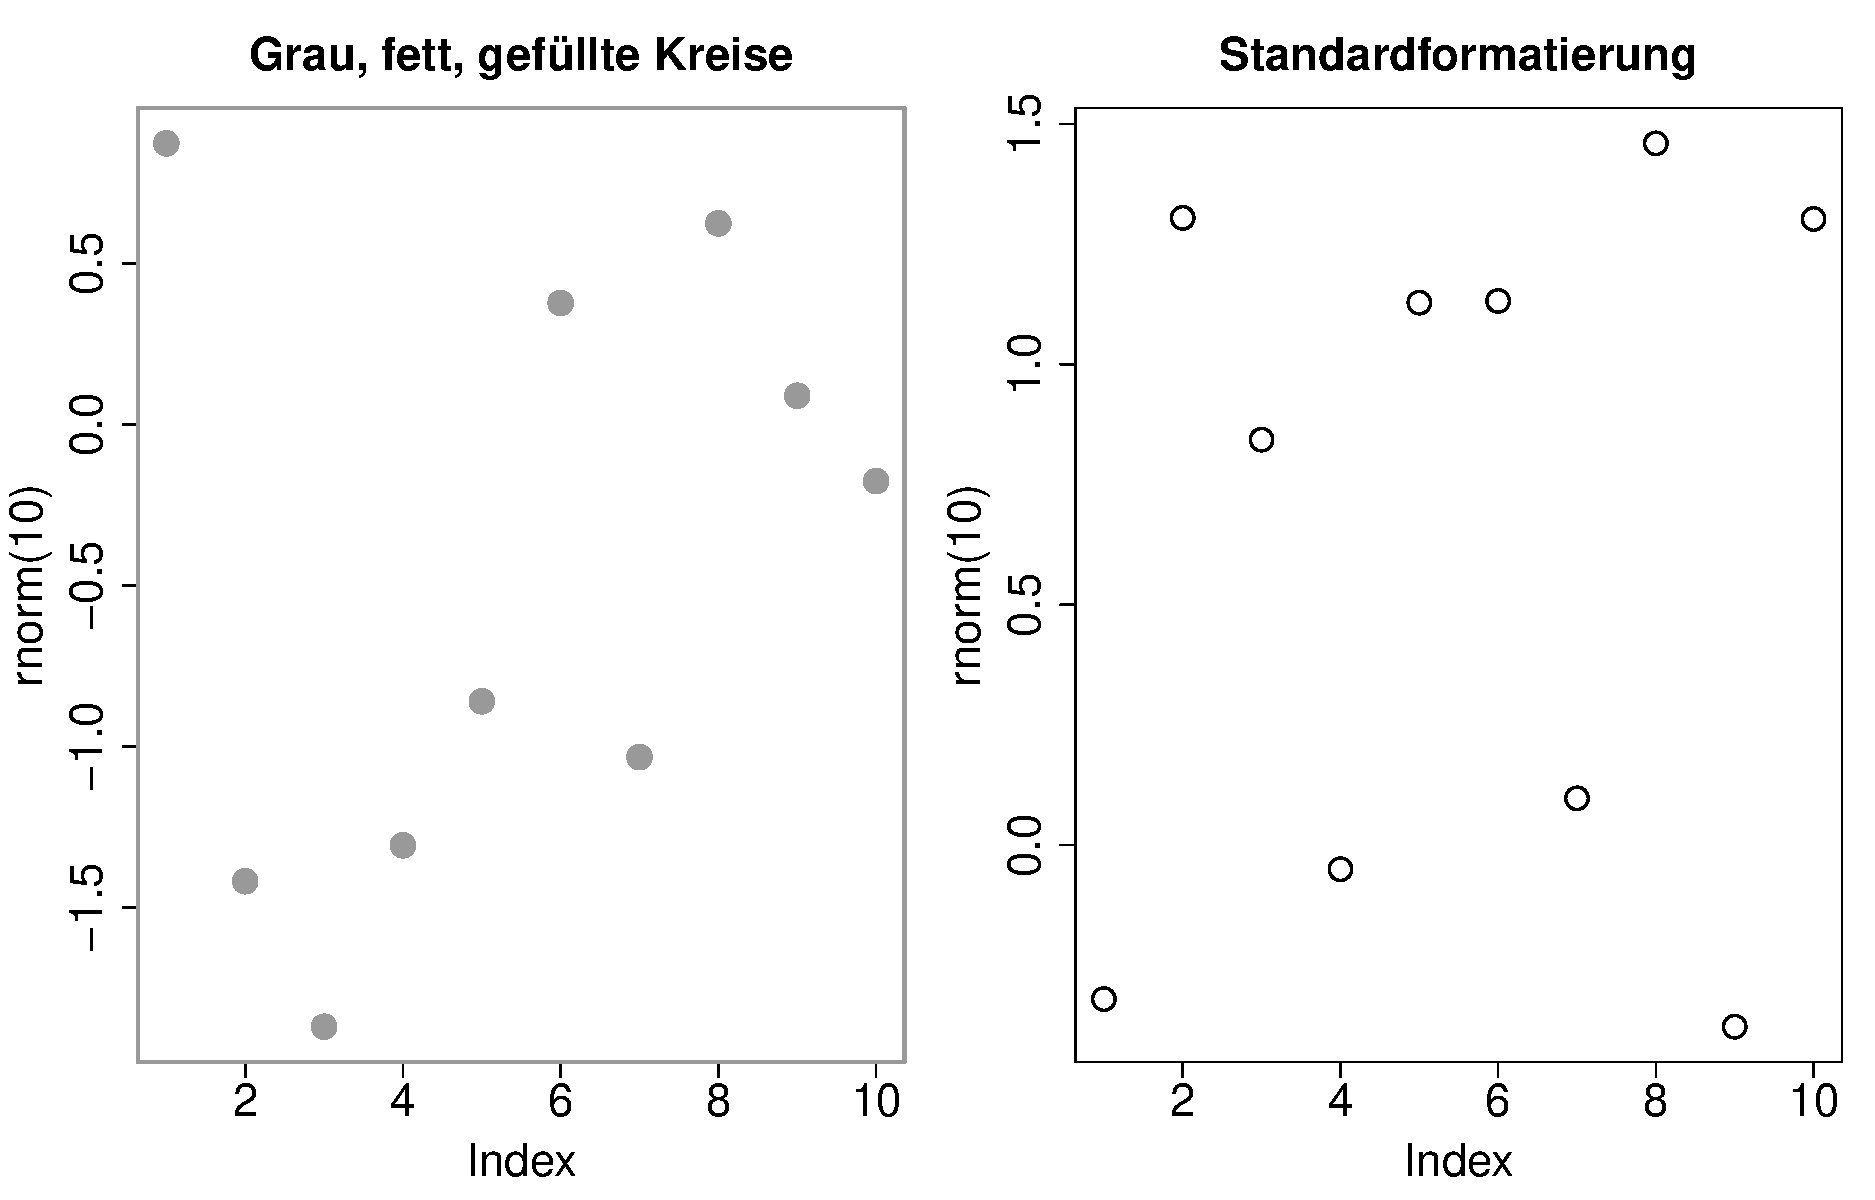
\includegraphics[width=12.5cm]{par}
\vspace*{-1em}
\caption{Verwendung von \lstinline!par()! zur Diagrammformatierung}
\label{fig:par}
\end{figure}

\index{Grafik!Linientypen}
\index{Grafik!Datenpunktsymbole}
Abbildung \ref{fig:pchLty} veranschaulicht die mit \lstinline!lty! und \lstinline!pch! einstellbaren Linientypen und Datenpunkt-Symbole (s.\ Abschn.\ \ref{sec:graphAddElem} für das Einfügen von Elementen in ein Diagramm). Symbole $21$--$25$ sind ausgefüllte Datenpunkte, deren Füllfarbe in Zeichenfunktionen über das Argument \lstinline!bg="<<Farbe>>"! definiert wird, während \lstinline!col="<<Farbe>>"! die Farbe des Randes bezeichnet (Abschn.\ \ref{sec:colors}).
\begin{lstlisting}
# Koordinaten der Datenpunkte
> X <- row(matrix(numeric(6*11), nrow=6, ncol=11))
> Y <- col(matrix(numeric(6*11), nrow=6, ncol=11))

# leeres Diagramm mit der richtigen Skalierung
> plot(0:6, seq(1, 11, length.out=7), type="n", axes=FALSE,
+      main="pch Datenpunkt-Symbole und lty Linientypen")

# Symbole für pch mit grauem Hintergrund für 21-25
> points(X[1:26], Y[1:26], pch=0:25, bg="gray", cex=2)

# Linien für lty
> matlines(X[ , 6:11], Y[ , 6:11], lty=6:1, lwd=2, col="black")

# erklärender Text - Nummer der pch Symbole und lty Linientypen
> text(X[1:26]-0.3, Y[1:26],    labels=0:25)
> text(rep(0.7, 6), Y[1, 6:11], labels=6:1)
> text(0, 9, labels="Linientypen für lty", srt=90, cex=1.2)
> text(0, 3, labels="Symbole für pch",     srt=90, cex=1.2)
\end{lstlisting}

\begin{figure}[ht]
\centering
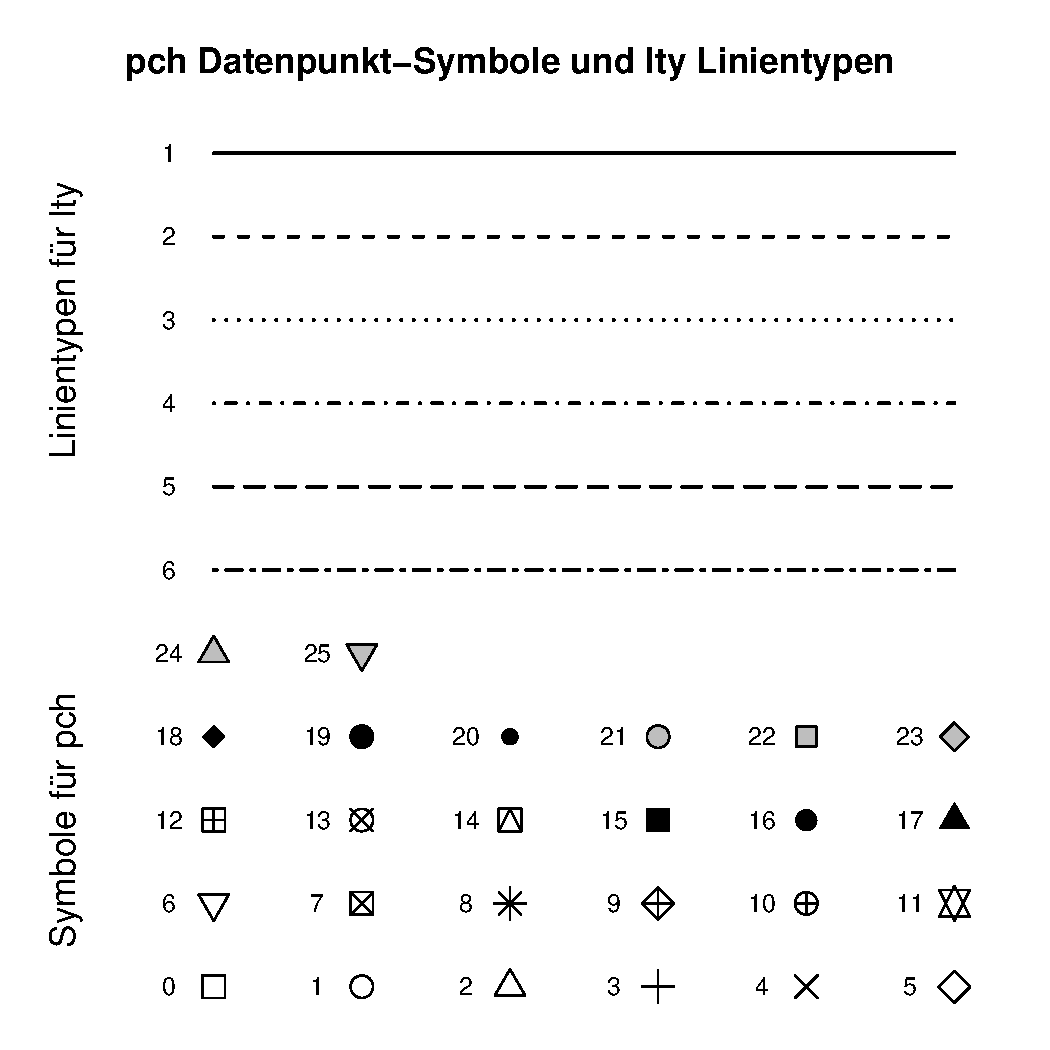
\includegraphics[width=8cm]{pchLty}
\vspace*{-1em}
\caption{Datenpunkt-Symbole und Linientypen zur Verwendung für die Argumente \lstinline!pch! und \lstinline!lty! von Grafikfunktionen}
\label{fig:pchLty}
\end{figure}

%%%%%%%%%%%%%%%%%%%%%%%%%%%%%%%%%%%%%%%%%%%%%%%%%%%%%%%%%%%%%%%%%%
%%%%%%%%%%%%%%%%%%%%%%%%%%%%%%%%%%%%%%%%%%%%%%%%%%%%%%%%%%%%%%%%%%
\subsection{Farben spezifizieren}
\label{sec:colors}
%%%%%%%%%%%%%%%%%%%%%%%%%%%%%%%%%%%%%%%%%%%%%%%%%%%%%%%%%%%%%%%%%%
%%%%%%%%%%%%%%%%%%%%%%%%%%%%%%%%%%%%%%%%%%%%%%%%%%%%%%%%%%%%%%%%%%

\index{Grafik!Farben}
\index{Farben|see{Grafik}}
Häufig ist es sinnvoll, Diagrammelemente farblich hervorzuheben, etwa um die Zusammengehörigkeit von Punkten innerhalb von Datenreihen zu kennzeichnen und verschiedene Datenreihen leichter voneinander unterscheidbar zu machen. Auch Text- und Hintergrundfarben können in Diagrammen frei gewählt werden. Zu diesem Zweck lassen sich Farben in unterschiedlicher Form an die entsprechenden Funktionsargumente (meist \lstinline!col!) übergeben:

\begin{itemize}
\item Als Farbname, z.\,B.\ \lstinline!"green"! oder \lstinline!"blue"!, vgl.\ \lstinline!colors()!\index[func]{colors()@\lstinline{colors()}} für mögliche Werte.
\item Im Hexadezimalformat, wobei die Intensitäten der Monitor-Grundfarben Rot, Grün und Blau in der Form \lstinline!"#RRGGBB"! mit Werten für \lstinline!RR!, \lstinline!GG! und \lstinline!BB! im Bereich von \lstinline!00! bis \lstinline!FF! angegeben werden. \lstinline!"#FF0000"! entspräche Rot, \lstinline!"#00FF00"! Grün.
\item Als natürliche Zahl, die als Index für die derzeit aktive Farbpalette interpretiert wird. Eine Farbpalette ist dabei ein vordefinierter Vektor von Farben, der mit\index[func]{palette()@\lstinline{palette()}} \lstinline!palette()! ausgegeben werden kann. Die voreingestellte Palette beginnt mit den Farben \lstinline!"black"!, \lstinline!"#DF536B"!, \lstinline!"#61D04F"!, -- der Index \lstinline!2! entspräche einem entsättigten Rot. Die Palette kann gewechselt werden, indem an \lstinline!palette(<<Vektor>>)! ein Vektor mit Farbnamen übergeben wird. Der (auf der Konsole unsichtbare) Rückgabewert enthält die ersetzte Palette und kann für einen temporären Wechsel der Palette in einem Vektor zwischengespeichert und später wieder an \lstinline!palette()! übergeben werden. Alternativ stellt \lstinline!palette("default")! die ursprünglich voreingestellte Palette wieder her. Für eine Beschreibung der verfügbaren Paletten vgl.\ \lstinline!?hcl.colors!. Die dort genannten Funktionen können etwa dazu eingesetzt werden, die aktive Farbpalette zu ändern, indem ihre Ausgabe an \lstinline!palette()! übergeben wird, z.\,B.\ mit \lstinline!palette(hcl.colors(10))!.\footnote{Das Paket \index[pack]{colorspace@\lstinline{colorspace}|textbf} \lstinline!colorspace! \cite{Zeileis2019, Ihaka2009} definiert eine Reihe von Paletten, deren Farben für besonders gute Unterscheidbarkeit unter verschiedenen Randbedingungen optimiert wurden -- etwa für Farbfehlsichtige oder Graustufen-Ausdrucke. Weiterführende Artikel zu diesem Thema nennt \lstinline!vignette("colorspace")!.}
\end{itemize}

\lstinline!col2rgb(<<Farbe>>)!\index[func]{col2rgb()@\lstinline{col2rgb()}} wandelt Farbnamen, Palettenindizes und Farben im Hexadezimalformat in einen Spaltenvektor um, der die Intensitäten der Monitor-Grundfarben Rot, Grün und Blau im Wertebereich von $0$--$255$ enthält. Namen und Hexadezimalzahlen müssen dabei in Anführungszeichen gesetzt werden. Da die Spezifizierung von Farben im Hexadezimalformat nicht sehr intuitiv ist, stellt R verschiedene Funktionen bereit, mit denen Farben auf einfachere Art definiert werden können. Diese Funktionen geben dann die bezeichnete Farbe im Hexadezimalformat aus.

\begin{itemize}
\item Mit\index[func]{rgb()@\lstinline{rgb()}} \lstinline!rgb(red=<<Rot>>, green=<<Grün>>, blue=<<Blau>>)! können die Intensitäten der Monitor-Grundfarben Rot, Grün und Blau mit Zahlen im Wertebereich von $0$--$1$ angegeben werden. Andere Höchstwerte lassen sich über das Argument \lstinline!maxColorValue! festlegen.\footnote{\label{ftn:transp}Ein vierter Wert zwischen $0$ und $1$ kann den Grad des\index{Grafik!Transparenz} \emph{alpha-blendings} für simulierte Transparenz definieren. Niedrige Werte stehen für sehr durchlässige, hohe Werte für opaque Farben (Abb.\ \ref{fig:pca}). Diese Art von Transparenz wird nur von manchen devices unterstützt, etwa von \lstinline!pdf()! oder \lstinline!png()!.} So gibt etwa \lstinline!rgb(0, 1, 1)! die Farbe \lstinline!"#00FFFF"! (Cyan) aus. Bei von \lstinline!col2rgb()! erzeugten Vektoren ist \lstinline!rgb()! mit dem Argument \lstinline!maxColorValue=255! zu verwenden.
\item Analog erzeugt\index[func]{hsv()@\lstinline{hsv()}} \lstinline!hsv(h=<<Farbton>>, s=<<Sättigung>>, v=<<Helligkeit>>)! (\emph{hue, saturation, value}) Farben, die mit Zahlen im Wertebereich von $0$--$1$ für Farbton, Sättigung und Helligkeit definiert werden.\footnote{Für weitere Funktionen zur Verwendung verschiedener Farbräume vgl.\  \index[func]{convertColor()@\lstinline{convertColor()}} \lstinline!?convertColor! sowie das Paket\index[pack]{colorspace@\lstinline{colorspace}} \lstinline!colorspace!.} So entspricht etwa \lstinline!hsv(0.1666, 1, 1)! der Farbe \lstinline!"#FFFF00"! (Gelb). \lstinline!rgb2hsv(r=<<Rot>>, g=<<Grün>>, b=<<Blau>>)!\index[func]{rgb2hsv()@\lstinline{rgb2hsv()}} rechnet von RGB-Farben in HSV-Werte um.
\item \lstinline!hcl(h=<<Farbton>>, c=<<Sättigung>>, l=<<Helligkeit>>)!\index[func]{hcl()@\lstinline{hcl()}} (\emph{hue, chroma, luminance}) erzeugt Farben im CIE Luv Koordinatensystem, das auf gleiche perzeptuelle Unterschiedlichkeit von im Farbraum gleich weit entfernten Farben abzielt. Dabei ist \lstinline!h! ein Winkel im Farbkreis im Bereich von $0$--$360^{\circ}$, \lstinline!c! die Sättigung, deren Höchstwert vom Farbton und der Luminanz abhängt und schließlich \lstinline!l! die Luminanz im Bereich von $0$--$100$.
\item \lstinline!gray(<<Grauwert>>)!\index[func]{gray()@\lstinline{gray()}} akzeptiert eine Zahl im Wertebereich von $0$--$1$, die als Helligkeit einer achromatischen Farbe mit identischen RGB-Werten interpretiert wird. So erzeugt etwa \lstinline!gray(0.5)! die graue Farbe \lstinline!"#808080"!. Das optionale Argument \lstinline!alpha! kontrolliert den Grad simulierter Transparenz (Fußnote \ref{ftn:transp}).
\item \lstinline!colorRamp(<<Farben>>)!\index[func]{colorRamp()@\lstinline{colorRamp()}} und \lstinline!colorRampPalette(<<Farben>>)!\index[func]{colorRampPalette()@\lstinline{colorRampPalette()}} erstellen einen Farbverlauf, indem sie im Farbraum gleichmäßig zwischen den übergebenen Farben interpolieren. Über das Argument \lstinline!alpha=TRUE! gilt dies auch für den Grad simulierter Transparenz. Das Ergebnis von \lstinline!colorRamp()! ist dabei eine Funktion, die ihrerseits eine Zahl im Bereich $[0,1]$ akzeptiert und als relative Distanz zwischen der ersten und letzten zu interpolierenden Farbe interpretiert. Dagegen ist die Ausgabe von \lstinline!colorRampPalette()! eine Funktion, die analog zu den vordefinierten Palettenfunktionen wie \lstinline!rainbow()! oder \lstinline!cm.colors()! arbeitet.
\item Eine gegebene Farbe kann mit \lstinline!adjustcolor()!\index[func]{adjustcolor()@\lstinline{adjustcolor()}} hinsichtlich verschiedener Attribute kontrolliert verändert werden -- etwa der Helligkeit, der Sättigung oder der simulierten Durchsichtigkeit.
\end{itemize}

%%%%%%%%%%%%%%%%%%%%%%%%%%%%%%%%%%%%%%%%%%%%%%%%%%%%%%%%%%%%%%%%%%
%%%%%%%%%%%%%%%%%%%%%%%%%%%%%%%%%%%%%%%%%%%%%%%%%%%%%%%%%%%%%%%%%%
\subsection{Achsen formatieren}
%%%%%%%%%%%%%%%%%%%%%%%%%%%%%%%%%%%%%%%%%%%%%%%%%%%%%%%%%%%%%%%%%%
%%%%%%%%%%%%%%%%%%%%%%%%%%%%%%%%%%%%%%%%%%%%%%%%%%%%%%%%%%%%%%%%%%

\index{Grafik!Achsen}
\begin{itemize}
\item Ob durch die Darstellung von Datenpunkten in einem Diagramm automatisch auch Achsen generiert werden, kontrollieren in High-Level-Funktionen die Argumente \lstinline!xaxt! für die $x$-Achse, \lstinline!yaxt! für die $y$-Achse und \lstinline!axes! für beide Achsen gleichzeitig. Während für \lstinline!xaxt! und \lstinline!yaxt! der Wert \lstinline!"n"! übergeben werden muss, um die Ausgabe der entsprechenden Achse zu unterdrücken, akzeptiert das Argument \lstinline!axes! dafür den Wert \lstinline!FALSE!\@.

\item Achsen können mit \lstinline!axis()! auch separat einem Diagramm hinzugefügt werden, wobei sich Lage, Beschriftung und Formatierung der Achsenmarkierungen festlegen lassen (Abschn.\ \ref{sec:axis}).

\item Die Argumente \lstinline!xlim=<<Vektor>>! und \lstinline!ylim=<<Vektor>>! von High-Level-Funktionen legen den durch die Achsen abgedeckten Wertebereich in Form eines Vektors mit dem kleinsten und größten Achsenwert fest. Fehlen diese Argumente, wird jeder Bereich automatisch anhand der darzustellenden Daten bestimmt.

\item Bei expliziten Angaben für \lstinline!xlim! oder \lstinline!ylim! gehen die Achsen auf beiden Seiten um $4\%$ über den angegebenen Wertebereich hinaus. Um dies zu verhindern, sind in High-Level-Funktionen die Argumente \lstinline!xaxs="i"! und \lstinline!yaxs="i"! zu setzen.

\item Die Achsenbezeichnungen können in High-Level-Funktionen über die Argumente \lstinline!xlab="<<Name>>"! und \lstinline!ylab="<<Name>>"! gewählt oder mit Setzen auf \lstinline!NA! unterdrückt werden.

\item Eine logarithmische Skalierung zur Basis $10$ lässt sich in High-Level-Funktionen getrennt für jede Achse mit dem Argument \lstinline!log="x"!, \lstinline!log="y"! bzw.\ für beide Achsen gemeinsam mit \lstinline!log="xy"! erzeugen.

\item Die Orientierung der Achsenmarkierungen legt das Argument \lstinline!las! von \lstinline!par()! fest. Senkrecht ausgerichtete Beschriftungen beanspruchen dabei häufig mehr vertikalen Platz, als es die Randeinstellungen vorsehen. Mit dem Argument \lstinline!mar! von \lstinline!par()! lässt sich der Rand zwischen Plot- und Figure-Region entsprechend anpassen.
\end{itemize}

%%%%%%%%%%%%%%%%%%%%%%%%%%%%%%%%%%%%%%%%%%%%%%%%%%%%%%%%%%%%%%%%%%
%%%%%%%%%%%%%%%%%%%%%%%%%%%%%%%%%%%%%%%%%%%%%%%%%%%%%%%%%%%%%%%%%%
\section{Säulen- und Punktdiagramme}
\label{sec:barplot}
%%%%%%%%%%%%%%%%%%%%%%%%%%%%%%%%%%%%%%%%%%%%%%%%%%%%%%%%%%%%%%%%%%
%%%%%%%%%%%%%%%%%%%%%%%%%%%%%%%%%%%%%%%%%%%%%%%%%%%%%%%%%%%%%%%%%%

\index{Grafik!Saeulendiagramm@Säulendiagramm}
\index{Grafik!Balkendiagramm}
\index{Balkendiagramm|see{Grafik}}
\index{Saulendiagramm@Säulendiagramm|see{Grafik}}
Mit\index[func]{barplot()@\lstinline{barplot()}} \lstinline!barplot()! erstellte Säulendiagramme eignen sich vor allem zur Darstellung absoluter oder relativer Häufigkeiten von Gruppenzugehörigkeiten. Die Häufigkeit jeder Gruppe wird dabei durch die Höhe einer Säule repräsentiert.

%%%%%%%%%%%%%%%%%%%%%%%%%%%%%%%%%%%%%%%%%%%%%%%%%%%%%%%%%%%%%%%%%%
%%%%%%%%%%%%%%%%%%%%%%%%%%%%%%%%%%%%%%%%%%%%%%%%%%%%%%%%%%%%%%%%%%
\subsection{Einfache Säulendiagramme}
%%%%%%%%%%%%%%%%%%%%%%%%%%%%%%%%%%%%%%%%%%%%%%%%%%%%%%%%%%%%%%%%%%
%%%%%%%%%%%%%%%%%%%%%%%%%%%%%%%%%%%%%%%%%%%%%%%%%%%%%%%%%%%%%%%%%%

Sollen allgemein Kennwerte einer Variable getrennt für Gruppen dargestellt werden, die sich aus den Stufen eines einzelnen Faktors ergeben, lautet die Grundform von \lstinline!barplot()!:
\begin{lstlisting}
barplot(height=<<Vektor>>, <<Argumente>>)
\end{lstlisting}

\begin{itemize}
\item Unter \lstinline!height! ist ein Vektor einzutragen, wobei jedes seiner Elemente den Kennwert für jeweils eine Bedingung repräsentiert und damit die Höhe einer Säule festlegt.
\item \lstinline!horiz! bestimmt, ob vertikale Säulen (Voreinstellung \lstinline!FALSE!) oder horizontale Balken gezeichnet werden. Der (auf der Konsole nicht sichtbare) Rückgabewert von \lstinline!barplot()! enthält die $x$-Koordinaten der eingezeichneten Säulen bzw.\ die $y$-Koordinaten der Balken.
\item \lstinline!space! legt den Abstand zwischen den Säulen fest, die Voreinstellung ist $0.2$.
\item \lstinline!names.arg! nimmt einen Vektor von Zeichenketten für die Beschriftung der Säulen an.
\item Ist das Minimum des mit \lstinline!ylim! definierten Wertebereichs der $y$-Achse größer als $0$, muss \lstinline!xpd=FALSE! gesetzt werden, um Säulen nicht unterhalb der $x$-Achse zeichnen zu lassen. Andernfalls erscheinen in der Voreinstellung \lstinline!xpd=TRUE! die Säulen unterhalb der $x$-Achse, auch wenn diese nicht bei $0$ beginnt.
\end{itemize}

Als Beispiel diene das Ergebnis mehrerer simulierter Würfe eines sechsseitigen Würfels, wobei einmal die absoluten und einmal die relativen Häufigkeiten dargestellt werden sollen (Abb.\ \ref{fig:barplot}).
\begin{lstlisting}
> dice  <- sample(1:6, 100, replace=TRUE)       # Würfelwürfe
> (dTab <- xtabs(~ dice)                        # absolute Häufigkeiten
dice
 1   2   3   4   5   61
17  23  14  20  14  12

> barplot(dTab, ylim=c(0, 30), xlab="Augenzahl", ylab="N", col="black",
+         main="Absolute Häufigkeiten")

> barplot(proportions(dTab), ylim=c(0, 0.3), xlab="Augenzahl",
+         ylab="relative Häufigkeit", col="gray50",
+         main="Relative Häufigkeiten")
\end{lstlisting}

\begin{figure}[ht]
\centering
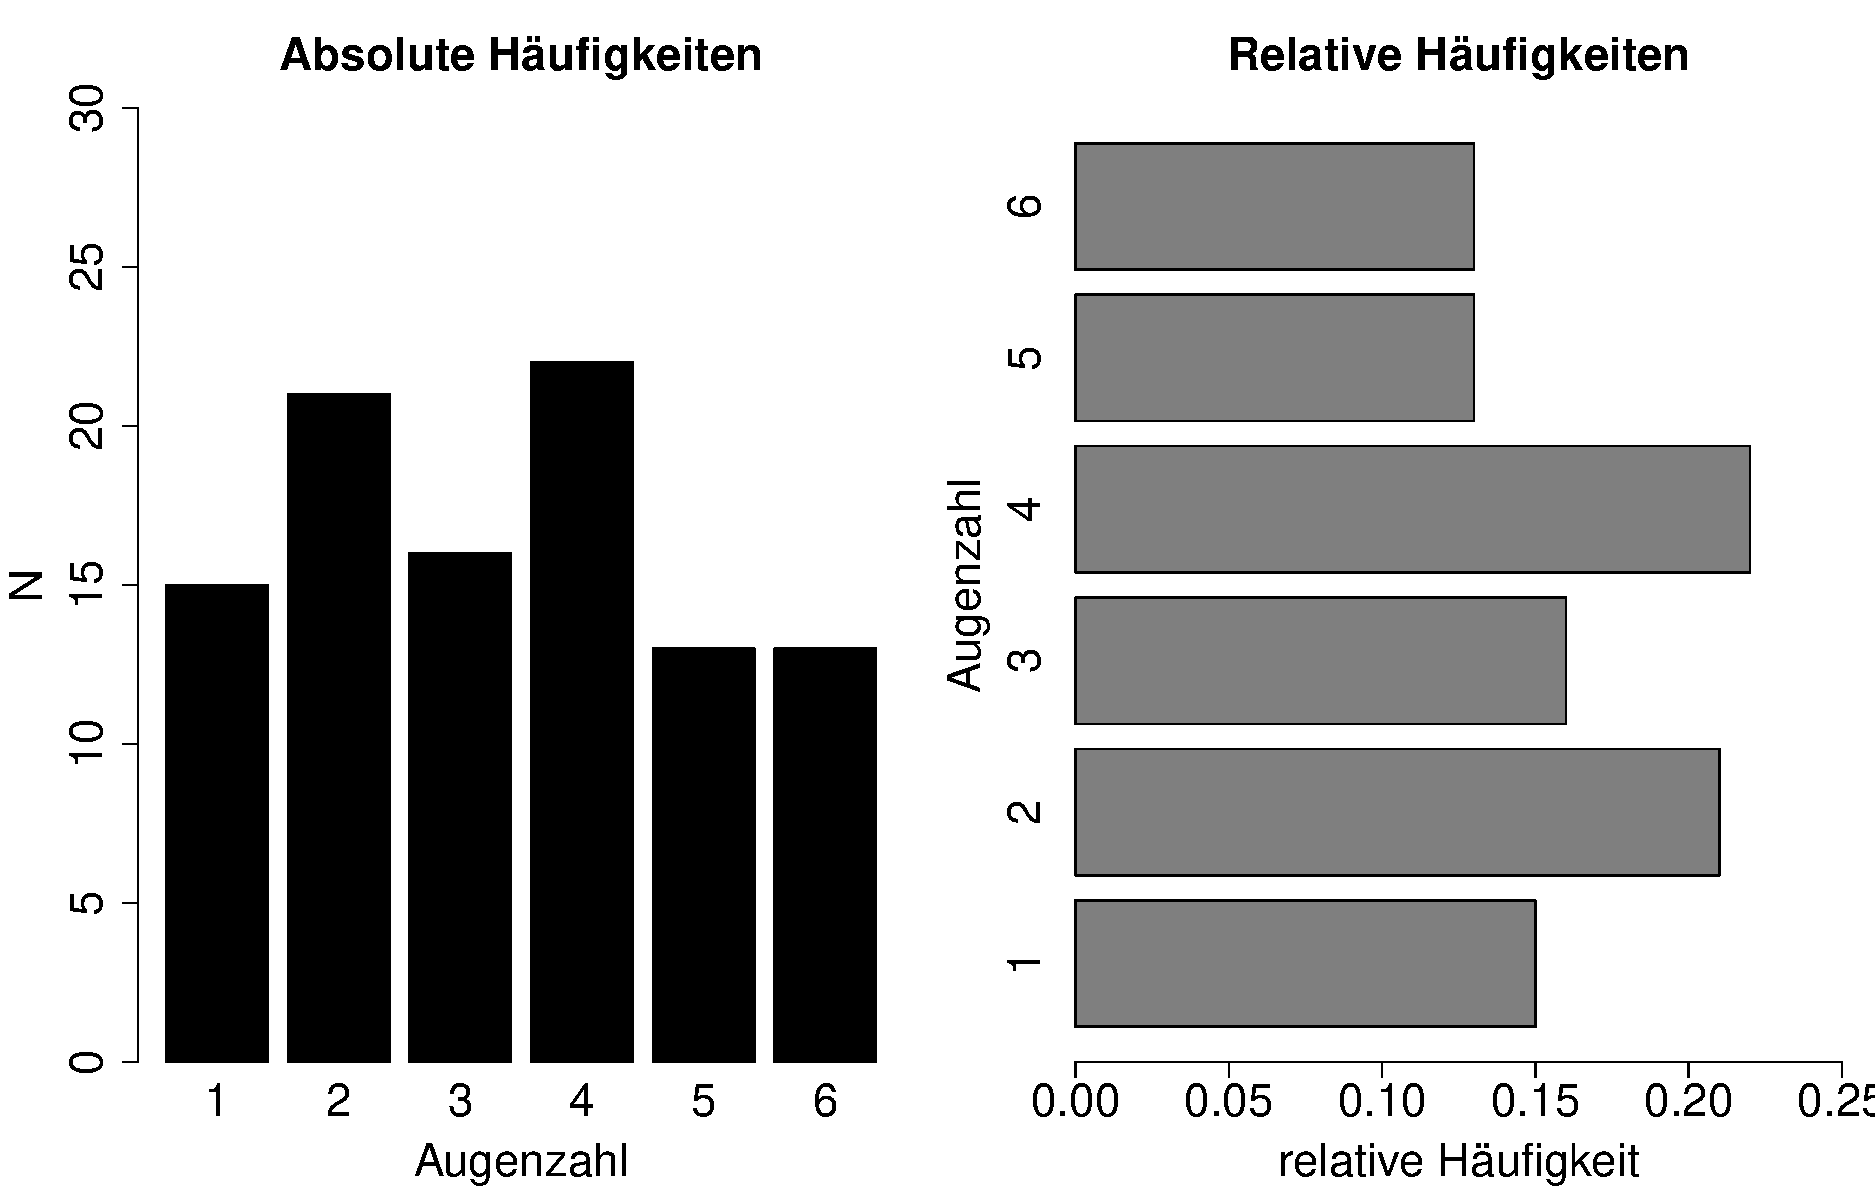
\includegraphics[width=12.5cm]{barplot}
\vspace*{-1em}
\caption{Säulendiagramme}
\label{fig:barplot}
\end{figure}

%%%%%%%%%%%%%%%%%%%%%%%%%%%%%%%%%%%%%%%%%%%%%%%%%%%%%%%%%%%%%%%%%%
%%%%%%%%%%%%%%%%%%%%%%%%%%%%%%%%%%%%%%%%%%%%%%%%%%%%%%%%%%%%%%%%%%
\subsection{Gruppierte und gestapelte Säulendiagramme}
\label{sec:barchartGroup}
%%%%%%%%%%%%%%%%%%%%%%%%%%%%%%%%%%%%%%%%%%%%%%%%%%%%%%%%%%%%%%%%%%
%%%%%%%%%%%%%%%%%%%%%%%%%%%%%%%%%%%%%%%%%%%%%%%%%%%%%%%%%%%%%%%%%%

\index{Grafik!Säulendiagramm}
Gruppierte Säulendiagramme stellen Kennwerte von Variablen getrennt für Gruppen dar, die sich aus der Kombination zweier Faktoren ergeben. Zu diesem Zweck kann die Zusammengehörigkeit einer aus mehreren Säulen bestehenden Gruppe grafisch durch ihre räumliche Nähe innerhalb der Gruppe und die gleichzeitig größere Distanz zu anderen Säulengruppen kenntlich gemacht werden. Eine weitere Möglichkeit besteht darin, jede Einzelsäule nicht homogen, sondern als Stapel mehrerer Segmente darzustellen (Abb.\ \ref{fig:barplotBeside}).

\begin{itemize}
\item Für gruppierte oder gestapelte Säulendiagramme werden die Daten an \lstinline!height! in Form einer Matrix übergeben, deren Werte die Säulenhöhen bzw.\ Balkenlängen festlegen.
\item Das Argument \lstinline!beside! kontrolliert, welche Darstellungsart gewählt wird: \lstinline!TRUE! steht für Säulengruppen, die Voreinstellung \lstinline!FALSE! für gestapelte Säulen.
\item Mit \lstinline!beside=FALSE! definiert jede Spalte der Datenmatrix die innere Zusammensetzung einer Säule, indem die einzelnen Werte einer Spalte die Höhe der Segmente bestimmen, aus denen die Säule besteht. Bei \lstinline!beside=TRUE! definiert eine Spalte der Datenmatrix eine Säulengruppe, deren jeweilige Höhen durch die Einzelwerte in der Spalte festgelegt sind.
\item Bei gruppierten Säulendiagrammen muss \lstinline!space! mit einem Vektor definiert werden. Das erste Element stellt den Abstand innerhalb der Gruppen dar, das zweite jenen zwischen den Gruppen. Voreinstellung ist der Vektor \lstinline!c(0, 1)!.
\item \lstinline!names.arg! nimmt einen Vektor von Zeichenketten an, der die Beschriftung der Säulengruppen definiert.
\item \lstinline!legend.text! kontrolliert, ob eine Legende eingefügt wird, Voreinstellung ist \lstinline!FALSE!\@. Auf \lstinline!TRUE! gesetzt erscheint eine Legende, die auf den Zeilennamen der Datenmatrix basiert und sich auf die Bedeutung der Säulen innerhalb einer Gruppe bzw.\ auf die Segmente einer Säule bezieht. Alternativ können die Einträge der Legende als Vektor von Zeichenketten angegeben werden.
\end{itemize}

\begin{lstlisting}
> roll1   <- dice[1:50]                  # erste Serie von Würfelwürfen
> roll2   <- dice[51:100]                # zweite Serie
> rollAll <- rbind(table(roll1), table(roll2))     # Matrix Gesamtdaten
> rownames(rollAll) <- c("first", "second")
> rollAll
         1   2  3   4  5  6
first    5  15  9   8  7  6
second  12   8  5  12  7  6
\end{lstlisting}

Die in jeder der sechs Gruppen vorhandenen zwei Säulen sollten farblich getrennt werden, um die Zugehörigkeit zur ersten bzw.\ zweiten Substichprobe deutlich zu machen. Dazu wird an \lstinline!col! ein Vektor mit zwei Farbnamen übergeben, den R intern so häufig recycled, wie es Säulengruppen gibt.
\begin{lstlisting}
> barplot(rollAll, beside=FALSE, legend.text=TRUE, xlab="Augenzahl",
+         ylab="N", main="Abs. Häufigkeiten in 2 Substichproben")

> barplot(rollAll, beside=TRUE, ylim=c(0, 15), col=c("red", "green"),
+         legend.text=TRUE, xlab="Augenzahl", ylab="N",
+         main="Abs. Häufigkeiten in 2 Substichproben")
\end{lstlisting}

\begin{figure}[ht]
\centering
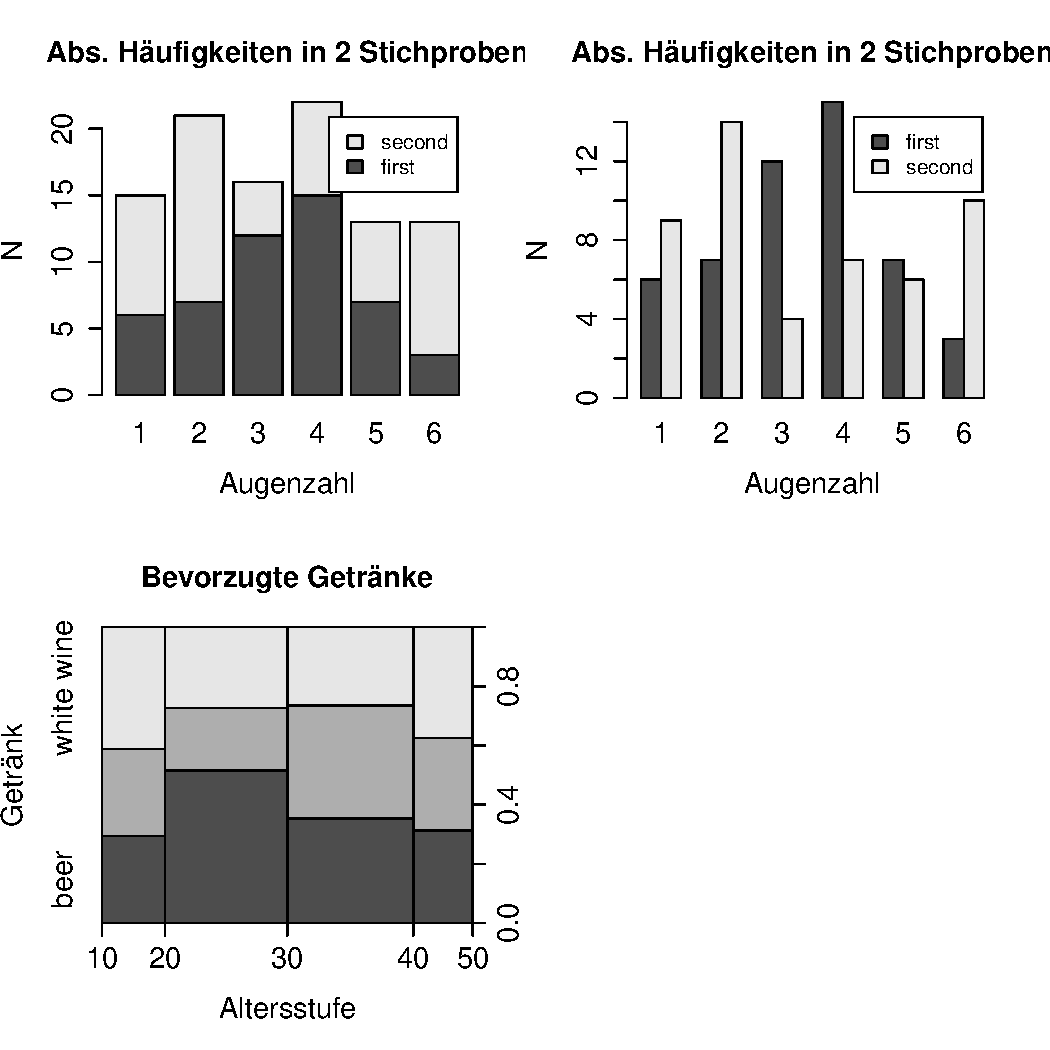
\includegraphics[width=12.5cm]{barplotBeside}
\vspace*{-1em}
\caption{Gestapeltes und gruppiertes Säulendiagramm absoluter sowie spineplot bedingter relativer Häufigkeiten}
\label{fig:barplotBeside}
\end{figure}

Eine Verallgemeinerung gestapelter Säulendiagramme, mit denen die bedingten relativen Häufigkeiten einer kategorialen Variable in Abhängigkeit von einer anderen Variable dargestellt werden können, erzeugt\index[func]{spineplot()@\lstinline{spineplot()}} \lstinline!spineplot()! (Abb.\ \ref{fig:barplotBeside}).\footnote{Für die Verteilung eines dichotomen Merkmals in Abhängigkeit einer kontinuierlichen Variable vgl.\ \index[func]{cdplot()@\lstinline{cdplot()}} \lstinline!cdplot()! (Abb.\ \ref{fig:regrLogCD}). Vergleiche \lstinline!mosaicplot()!\index[func]{mosaicplot()@\lstinline{mosaicplot()}} (Abb.\ \ref{fig:loglinUCBA}) für die gemeinsame Verteilung von mehr als zwei kategorialen Variablen.}
\begin{lstlisting}
spineplot(x=<<Vektor>>, y=<<Faktor>>, breaks=<<Grenzen>>,
          xaxlabels="<<Bezeichnungen>>", yaxlabels="<<Bezeichnungen>>")
\end{lstlisting}

Die Daten in \lstinline!x! und \lstinline!y! gelten als Werte, die an denselben Beobachtungsobjekten erhoben wurden. Im Fall von \lstinline!x! sind dies entweder Ausprägungen einer kategorialen (\lstinline!x! ist ein Faktor) oder einer quantitativen Variable (\lstinline!x! ist ein numerischer Vektor), während \lstinline!y! ein Faktor sein muss. Das Diagramm setzt sich aus nahtlos nebeneinander stehenden Säulen zusammen, deren Anzahl sowie Breite durch \lstinline!x! und deren Aufteilung in Segmente durch \lstinline!y! definiert ist: Sofern \lstinline!x! ein Faktor ist, stellt das Diagramm für jede seiner Ausprägungen eine Säule dar, die aus so vielen Segmenten besteht, wie \lstinline!y! Ausprägungen hat. Der Flächeninhalt eines Segments spiegelt die relative Häufigkeit der zugehörigen Stufenkombination in der Gesamtstichprobe wider. Die bedingten relativen Häufigkeiten der Stufen von \lstinline!y! in der Stufe von \lstinline!x! werden dabei über die Höhe der Segmente visualisiert. Die Breite der Säulen repräsentiert die relativen Häufigkeiten der Stufen von \lstinline!x!, so dass insgesamt die Verteilungen beider Variablen im Diagramm abzulesen sind.

Ist \lstinline!x! eine quantitative Variable, wird ihr Wertebereich zunächst entweder automatisch in disjunkte Intervalle eingeteilt, oder anhand eines für \lstinline!breaks! übergebenen Vektors mit den Intervallgrenzen. Alternativ kann für \lstinline!x! und \lstinline!y! zum einen eine Modellformel der Form \lstinline!<<y>> ~ <<x>>! genannt werden. Zum anderen lassen sich die Daten in Gestalt einer zweidimensionalen Kreuztabelle der gemeinsamen Häufigkeiten von \lstinline!x! und \lstinline!y! übergeben -- diese Kreuztabelle ist gleichzeitig der auf der Konsole nicht sichtbare Rückgabewert von \lstinline!spineplot()!. Die Bezeichnungen für die durch \lstinline!x! und \lstinline!y! definierten Bedingungen ergeben sich aus deren Faktorstufen, können aber auch explizit durch Vektoren aus Zeichenketten für \lstinline!xaxlabels! und \lstinline!yaxlabes! genannt werden.

Die folgenden Daten simulieren das Ergebnis einer Umfrage, in der Personen unterschiedlichen Alters ihre Präferenz für ein alkoholisches Getränk nennen.
\begin{lstlisting}
> N      <- 100                                     # Anzahl Personen
> age    <- sample(18:45, N, replace=TRUE)          # Alter
> drinks <- c("beer", "red wine", "white wine")     # mögliche Getränke
> pref   <- factor(sample(drinks, N, replace=TRUE)) # Präferenzen

# Intervallgrenzen zur Diskretisierung von age
> xRange <- round(range(age), -1) + c(-10, 10)
> lims   <- seq(xRange[1], xRange[2], by=10)
> spineplot(x=age, y=pref, xlab="Altersstufe", ylab="Getränk",
+           breaks=lims, main="Bevorzugte Getränke pro Altersstufe")
\end{lstlisting}

%%%%%%%%%%%%%%%%%%%%%%%%%%%%%%%%%%%%%%%%%%%%%%%%%%%%%%%%%%%%%%%%%%
%%%%%%%%%%%%%%%%%%%%%%%%%%%%%%%%%%%%%%%%%%%%%%%%%%%%%%%%%%%%%%%%%%
\subsection{Dotchart}
%%%%%%%%%%%%%%%%%%%%%%%%%%%%%%%%%%%%%%%%%%%%%%%%%%%%%%%%%%%%%%%%%%
%%%%%%%%%%%%%%%%%%%%%%%%%%%%%%%%%%%%%%%%%%%%%%%%%%%%%%%%%%%%%%%%%%

\index{Grafik!Punktdiagramm}
\index{Grafik!dotchart}
\index[func]{dotchart()@\lstinline{dotchart()}}
\lstinline!dotchart()! dient der Darstellung von Rohdaten einzelner Beobachtungsobjekte, aber auch von aggregierten Kennwerten von Variablen. Dies können etwa absolute oder relative Häufigkeiten von Gruppenzugehörigkeiten oder die jeweiligen Mittelwerte einer Variable in verschiedenen Stichproben sein. Jeder Wert wird dabei durch einen Punkt repräsentiert, dessen $x$-Koordinate seine Größe widerspiegelt und dessen $y$-Koordinate das Beobachtungsobjekt codiert. Das Ergebnis von \lstinline!dotchart()! ist analog zu einem horizontalen Balkendiagramm, wobei statt der Balken lediglich Punkte eingezeichnet werden.
\begin{lstlisting}
dotchart(x=<<Daten>>, labels="<<Namen>>", groups=<<Faktor>>, gdata=<<Daten>>)
\end{lstlisting}

Für \lstinline!x! ist der Datenvektor anzugeben. Über das Argument \lstinline!labels! lassen sich mittels eines Vektors aus Zeichenketten derselben Länge wie \lstinline!x! die Bezeichnungen der Datenpunkte nennen. Sollen Daten aus verschiedenen, durch die Kombination zweier Faktoren gebildeten Gruppen dargestellt werden, sind die Daten in Form einer Matrix zu übergeben, deren Werte die $x$-Koordinaten der Punkte festlegen. Dabei definiert jede Spalte der Datenmatrix eine Punktgruppe, deren Punkte vertikal nahe beieinander gezeichnet werden, wohingegen die durch verschiedene Spalten definierten Punkte stärker räumlich getrennt sind.

Stellen die Daten Kennwerte verschiedener Gruppen dar, können sie auch als Vektor \lstinline!x! unter gleichzeitiger Angabe von \lstinline!groups! übergeben werden. Für \lstinline!groups! ist dann ein Faktor derselben Länge wie \lstinline!x! zu nennen, der die Gruppenzugehörigkeit jedes Wertes definiert -- auf diese Weise lassen sich auch Daten ungleich großer Gruppen darstellen. Zusätzlich zu den in \lstinline!x! enthaltenen Werten lassen sich für \lstinline!gdata! weitere Daten in Form eines Vektors mit so vielen Elementen angeben, wie Gruppen vorhanden sind. Jeder Wert von \lstinline!gdata! wird als zu jeweils einer Gruppe gehörig interpretiert und als einzelner Vergleichswert eingezeichnet. Diese Möglichkeit ist z.\,B.\ geeignet, um neben den Rohdaten einer Gruppe gleichzeitig auch einen aggregierten Kennwert der Daten mit darzustellen (Abb.\ \ref{fig:dotchart}).
\begin{lstlisting}
> Nj  <- 5                                       # Gruppengröße
> DV1 <- rnorm(Nj, 20, 2)                        # Daten Gruppe 1
> DV2 <- rnorm(Nj, 25, 2)                        # Daten Gruppe 2
> DV  <- c(DV1, DV2)                             # Gesamt-Daten
> IV  <- gl(2, Nj)                               # Gruppenzugehörigkeit
> Mj  <- tapply(DV, IV, mean)                    # Gruppenmittel
> dotchart(DV, gdata=Mj, pch=rep(c(17, 19), each=Nj),
+          color=rep(c("red", "blue", "green"), each=Nj),
+          gcolor="black", groups=IV, labels=rep(LETTERS[1:Nj], 2),
+          xlab="Messwerte", ylab="Gruppen",
+          main="Individuelle Ergebnisse und Mittel aus 2 Gruppen")
\end{lstlisting}

\begin{figure}[ht]
\centering
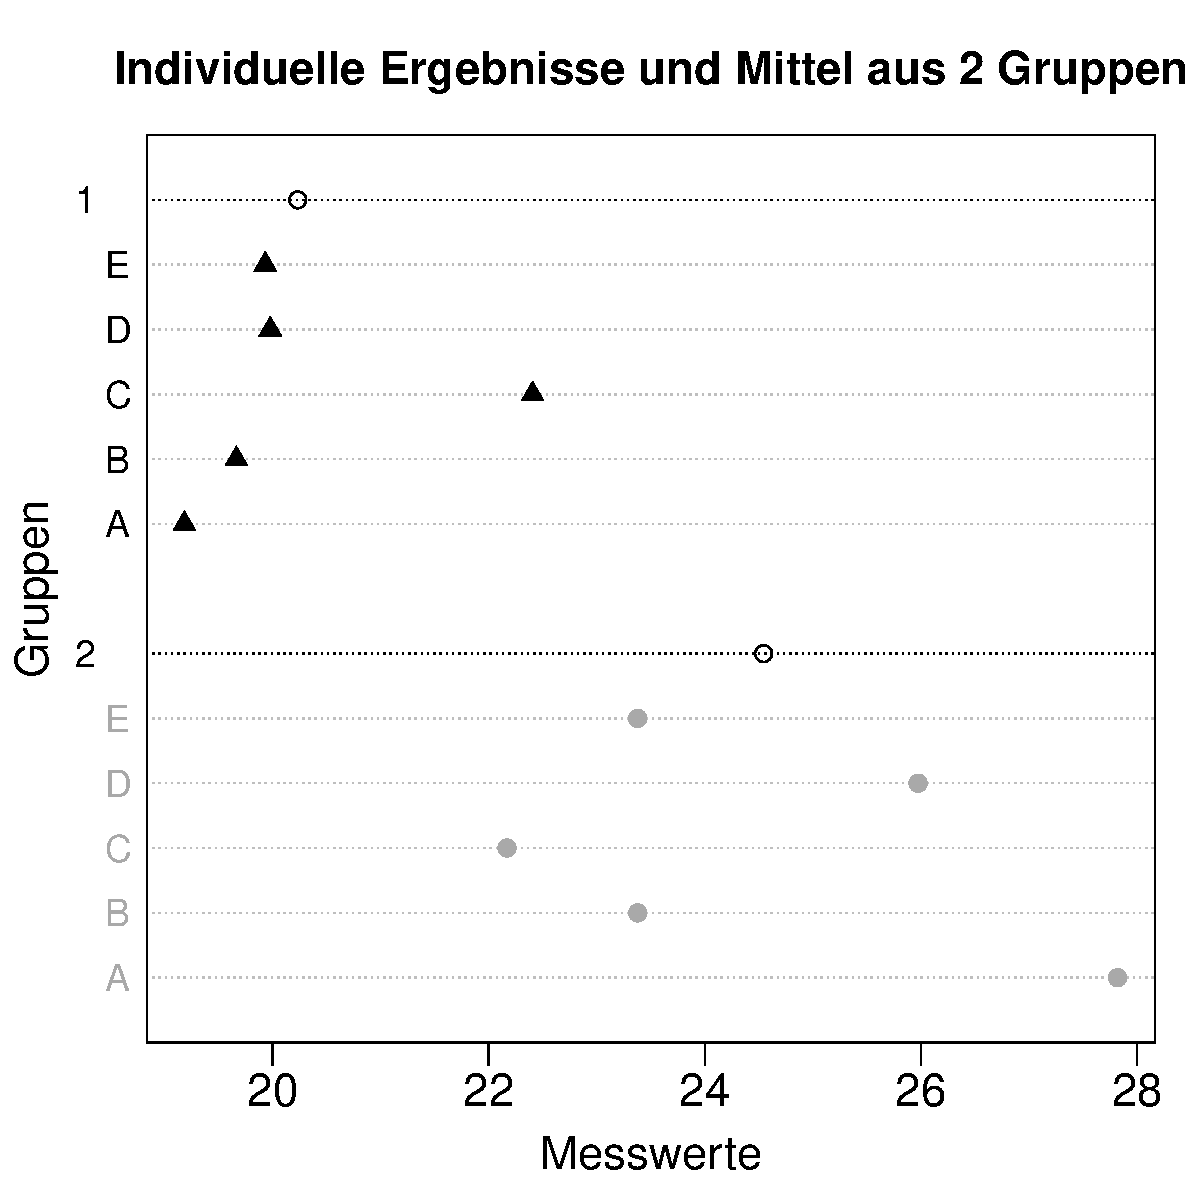
\includegraphics[width=8cm]{dotchart}
\vspace*{-1em}
\caption{Dotchart von individuellen Messwerten in zwei Gruppen samt zugehöriger Mittelwerte}
\label{fig:dotchart}
\end{figure}

%%%%%%%%%%%%%%%%%%%%%%%%%%%%%%%%%%%%%%%%%%%%%%%%%%%%%%%%%%%%%%%%%%
%%%%%%%%%%%%%%%%%%%%%%%%%%%%%%%%%%%%%%%%%%%%%%%%%%%%%%%%%%%%%%%%%%
\section{Elemente einem bestehenden Diagramm hinzufügen}
\label{sec:graphAddElem}
%%%%%%%%%%%%%%%%%%%%%%%%%%%%%%%%%%%%%%%%%%%%%%%%%%%%%%%%%%%%%%%%%%
%%%%%%%%%%%%%%%%%%%%%%%%%%%%%%%%%%%%%%%%%%%%%%%%%%%%%%%%%%%%%%%%%%

\index{Grafik!Elemente hinzufügen}
Ein bereits erstelltes Diagramm lässt sich nachträglich durch zusätzliche Elemente erweitern, die durch\index{Grafik!Low-Level-Funktion} Low-Level-Funktionen erzeugt werden (Tab.\ \ref{tab:addGraphElems}). Auch einige\index{Grafik!High-Level-Funktion} High-Level-Funktionen besitzen das Argument \lstinline!add=TRUE!, durch das ihre Ausgabe dem derzeit aktiven device hinzugefügt wird, ohne dessen Inhalte zuvor zu löschen. In diesem Fall kann meist durch das Argument \lstinline!at=<<Position>>! bestimmt werden, an welcher Stelle der Plot-Region die zusätzlichen Daten erscheinen sollen. Ist kein \lstinline!add! Argument vorhanden, bewirkt die vorhergehende Ausführung von \lstinline!par(new=TRUE)!, dass das Ergebnis des folgenden High-Level-Befehls im schon geöffneten device erscheint. Später eingefügte Elemente werden immer über bereits bestehende gezeichnet -- neue Inhalte übermalen also ältere Inhalte, die sich an derselben Stelle befinden.

%\begin{longtable}{p{3.5cm}p{9.5cm}}
\begin{table}[ht]
\centering
\caption{Mögliche Diagrammelemente und die sie hinzufügenden Funktionen}
\label{tab:addGraphElems}
\begin{tabular}{p{3.5cm}p{9cm}}
\hline
\sffamily Diagrammelement & \sffamily hinzufügende Low-Level-Grafikfunktion\\\hline\hline
Punkte & \lstinline!points()!, \lstinline!matpoints()!\\
Geradenabschnitte & \lstinline!lines()!, \lstinline!matlines()!, \lstinline!segments()!, \lstinline!abline()!\\
Gitter, Pfeile & \lstinline!grid()!, \lstinline!arrows()!\\
Polygone & \lstinline!box()!, \lstinline!rect()!, \lstinline!polygon()!\\
interpolierte Punkte & \lstinline!approx()!, \lstinline!spline()!, \lstinline!smooth.spline()!, \lstinline!xspline()!\\
                     & Abschn.\ \ref{sec:interpolate}\\
Funktionsgraphen & \lstinline!curve()!\\
Text & \lstinline!title()!, \lstinline!legend()!, \lstinline!text()!, \lstinline!mtext()!\\
Achsen & \lstinline!axis()!\\\hline
\end{tabular}
\end{table}
%\end{longtable}

Die Verwendung von Low-Level-Funktionen setzt voraus, dass bereits ein Diagramm mit einer High-Level-Funktion erstellt wurde. Um diesen Schritt zu überspringen und ein Diagramm ausschließlich aus Low-Level-Funktionen aufzubauen, kann aber auch ein device mit \lstinline!dev.new()! sowie anschließend\index[func]{plot.new()@\lstinline{plot.new()}} \lstinline!plot.new()! geöffnet und zum Einfügen von Elementen vorbereitet werden.

%%%%%%%%%%%%%%%%%%%%%%%%%%%%%%%%%%%%%%%%%%%%%%%%%%%%%%%%%%%%%%%%%%
%%%%%%%%%%%%%%%%%%%%%%%%%%%%%%%%%%%%%%%%%%%%%%%%%%%%%%%%%%%%%%%%%%
\subsection{Koordinaten in einem Diagramm identifizieren}
%%%%%%%%%%%%%%%%%%%%%%%%%%%%%%%%%%%%%%%%%%%%%%%%%%%%%%%%%%%%%%%%%%
%%%%%%%%%%%%%%%%%%%%%%%%%%%%%%%%%%%%%%%%%%%%%%%%%%%%%%%%%%%%%%%%%%

\index{Grafik!Koordinaten identifizieren}
Die meisten nachträglich einzufügenden Diagrammelemente erfordern für ihre Positionierung die Angabe von $(x, y)$-Koordinaten in einem Koordinatensystem, das durch die in der Plot-Region (Abschn.\ \ref{sec:device}, Abb.\ \ref{fig:margins}) bereits dargestellten Daten festgelegt ist. Diese \emph{User}-Koordinaten neu einzufügender Elemente ergeben sich oft direkt aus den Daten, mitunter soll ein Element aber auch frei plaziert werden. Eine Alternative zur Bestimmung der dafür geeigneten Koordinaten durch Versuch und Irrtum bietet\index[func]{locator()@\lstinline{locator()}} \lstinline!locator(n=<<Anzahl>>)!, nachdem ein Diagrammfenster erstellt wurde und noch geöffnet ist.

Das Argument \lstinline!n! legt fest, wie viele Koordinaten zu bestimmen sind. Durch den Aufruf von \lstinline!locator()! ändert sich der Mauszeiger zu einem Kreuz, sobald er sich über der Diagrammfläche befindet. Mit einem Klick der linken Maustaste werden die Koordinaten der Mausposition zwischengespeichert, währenddessen ist die Konsole für Eingaben blockiert. Der Vorgang kann mehrfach wiederholt werden und endet entweder, nachdem $n$ Punkte gespeichert wurden, oder über ein sich durch Klicken der rechten Maustaste öffnendes Kontextmenü (in RStudio durch Drücken der \lstinline[language=]!ESC! Taste). Daraufhin gibt \lstinline!locator()! eine Liste mit den Komponenten \lstinline!x! und \lstinline!y! zurück, die in Form jeweils eines Vektors die $(x, y)$-Koordinaten der angeklickten Punkte enthalten.
\begin{lstlisting}
> plot(rnorm(10))                   # Streudiagramm
> (xy <- locator(n=3))              # 3 Punkte durch Klicken auswählen
$x
[1] 2.402735 7.008204 3.141016

$y
[1] 0.656082382 -0.006072532 -0.484488124
\end{lstlisting}

%%%%%%%%%%%%%%%%%%%%%%%%%%%%%%%%%%%%%%%%%%%%%%%%%%%%%%%%%%%%%%%%%%
%%%%%%%%%%%%%%%%%%%%%%%%%%%%%%%%%%%%%%%%%%%%%%%%%%%%%%%%%%%%%%%%%%
\subsection{In beliebige Diagrammbereiche zeichnen}
\label{sec:clipping}
%%%%%%%%%%%%%%%%%%%%%%%%%%%%%%%%%%%%%%%%%%%%%%%%%%%%%%%%%%%%%%%%%%
%%%%%%%%%%%%%%%%%%%%%%%%%%%%%%%%%%%%%%%%%%%%%%%%%%%%%%%%%%%%%%%%%%

\index{Grafik!Koordinatensysteme}
\index{Grafik!clipping}
Die Voreinstellungen für ein device legen fest, dass zusätzliche Elemente nur in der Plot-Region gezeichnet werden können (Abschn.\ \ref{sec:device}, Abb.\ \ref{fig:margins}). Diese \emph{clipping} genannte Beschränkung kann über das Argument \lstinline!xpd=NA! von \lstinline!par()! aufgehoben werden (Abb.\ \ref{fig:clipping}). Für zusätzliche Grafikelemente müssen auch außerhalb der Plot-Region letztlich User-Koordinaten verwendet werden, die durch die bereits dargestellten Daten definiert sind. Die einzelnen Device-Regionen besitzen jedoch auch eigene Koordinatensysteme, die es erlauben, allgemeingültige Koordinaten zur Plazierung von Elementen zu verwenden, die unabhängig von den konkreten Daten sind: Die Ränder jeder Device-Region definieren dafür jeweils ein Rechteck mit $(x, y)$-Koordinaten im Bereich $0$--$1$, wobei $(0, 0)$ die linke untere und $(1, 1)$ die rechte obere Ecke bezeichnet. Diese Koordinaten müssen vor der Darstellung eines Elements in User-Koordinaten umgewandelt werden, wozu\index[func]{cnvrt.coords()@\lstinline{cnvrt.coords()}} \lstinline!cnvrt.coords()! aus dem Paket\index[pack]{Hmisc@\lstinline{Hmisc}} \lstinline!Hmisc! dient.
\begin{lstlisting}
cnvrt.coords(x=<<x-Koordinaten>>, y=<<y-Koordinaten>>,
             input=c("usr", "plt", "fig", "dev", "tdev"))
\end{lstlisting}

Unter \lstinline!x! und \lstinline!y! sind die $x$ bzw.\ $y$-Koordinaten der einzuzeichnenden Elemente jeweils als Vektor einzutragen. Auf welches Koordinatensystem sie sich beziehen, legt das Argument \lstinline!input! fest. Dabei steht \lstinline!"usr"! für User-Koordinaten, \lstinline!"plt"! für Koordinaten der Plot-Region, entsprechend \lstinline!"fig"! für die Figure-Region, \lstinline!"dev"! für die Device-Region ohne die äußeren Ränder und \lstinline!"tdev"! für die Device-Region inkl.\ dieser Ränder.

\lstinline!cnvrt.coords()! gibt eine Liste zurück, die für jedes Koordinatensystem eine Komponente mit den konvertierten Koordinaten besitzt. Die Komponenten tragen dabei dieselben Namen wie die möglichen Werte für das Argument \lstinline!input!. Jede Komponente ist wiederum eine Liste mit den Komponenten \lstinline!x! und \lstinline!y! für die $(x, y)$-Koordinaten.
\begin{lstlisting}
# clipping ausschalten und äußere Ränder setzen
> par(xpd=NA, oma=c(2, 2, 2, 2))
> plot(rnorm(10), xlab=NA, ylab=NA, pch=20)        # Streudiagramm
> library(Hmisc)                                   # für cnvrt.coords()

# Figure-Region links-unten
> pt1 <- cnvrt.coords(0, 0, input="fig")           # Figure-Koordinaten
> pt1$usr                                          # User-Koordinaten
$x
[1] -0.9669358

$y
[1] -3.389251

# Kreuz und zugehörigen Text einfügen
> points(pt1$usr, pch=4, lwd=5, cex=5, col="darkgray")
> text(pt1$usr$x + 0.5, pt1$usr$y, adj=c(0, 0), cex=1.5,
+      labels="Kreuz links-unten Figure-Region")

# gesamte Device-Region links-oben und rechts-unten
> pt2 <- cnvrt.coords(c(0.05, 0.95), c(0.95, 0.05), input="tdev")
> pt2$usr                                           # User-Koordinaten
$x
[1] -1.064920 11.281049

$y
[1] 2.163520 -3.433674

# Pfeil und Text einfügen
> arrows(x0=pt2$usr$x[1], y0=pt2$usr$y[1], x1=pt2$usr$x[2],
+        y1=pt2$usr$y[2], lwd=4, code=3, angle=90, lend=2,
+        col="darkgray")

> text(pt2$usr$x[1] + 0.5, pt2$usr$y[1], adj=c(0, 0), cex=1.5,
+      labels="Pfeil über gesamte Device-Region")
\end{lstlisting}

\begin{figure}[ht]
\centering
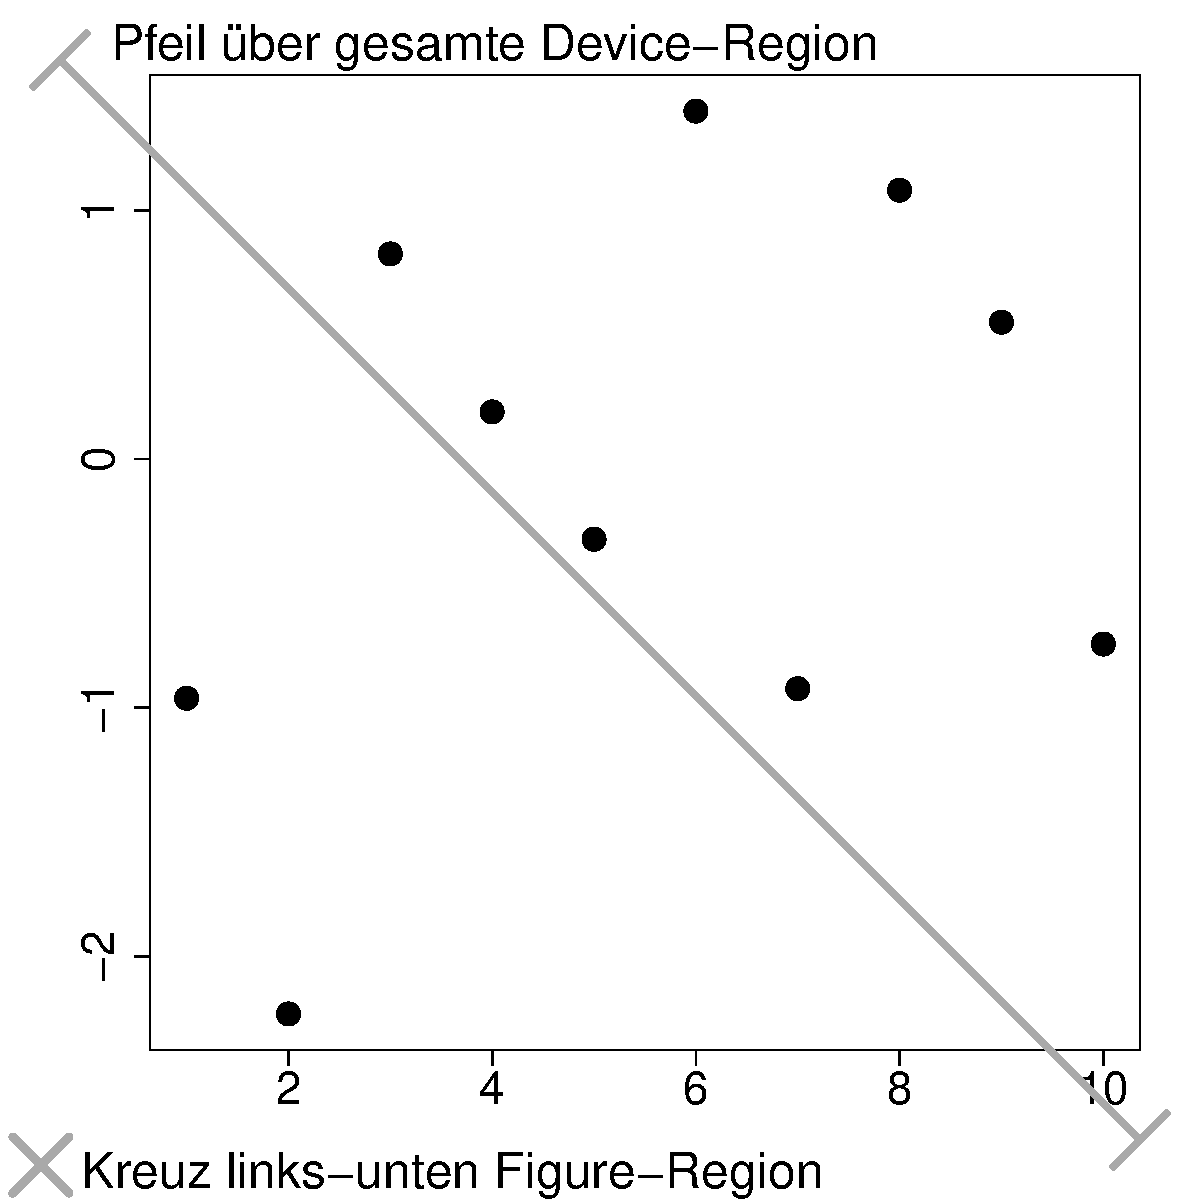
\includegraphics[width=8cm]{clipping}
\vspace*{-0.5em}
\caption{Grafikelemente an beliebiger Stelle eines Diagramms einfügen}
\label{fig:clipping}
\end{figure}

%%%%%%%%%%%%%%%%%%%%%%%%%%%%%%%%%%%%%%%%%%%%%%%%%%%%%%%%%%%%%%%%%%
%%%%%%%%%%%%%%%%%%%%%%%%%%%%%%%%%%%%%%%%%%%%%%%%%%%%%%%%%%%%%%%%%%
\subsection{Punkte}
%%%%%%%%%%%%%%%%%%%%%%%%%%%%%%%%%%%%%%%%%%%%%%%%%%%%%%%%%%%%%%%%%%
%%%%%%%%%%%%%%%%%%%%%%%%%%%%%%%%%%%%%%%%%%%%%%%%%%%%%%%%%%%%%%%%%%

\index{Grafik!Punkte}
\index[func]{points()@\lstinline{points()}}
\index[func]{matpoints()@\lstinline{matpoints()}}
\begin{lstlisting}
points(x=<<x-Koordinaten>>, y=<<y-Koordinaten>>, type="<<Option>>")
matpoints(x=<<Matrix>>, y=<<Matrix>>, type="<<Option>>")
\end{lstlisting}

Ähnlich wie \lstinline!plot()! fügt \lstinline!points()! einem geöffneten Diagramm Punkte hinzu, die Argumente \lstinline!x!, \lstinline!y! und \lstinline!type! stimmen in ihrer Bedeutung mit jenen von \lstinline!plot()! überein. Analog zu \lstinline!matplot()! können mit \lstinline!matpoints()! für $x$- und $y$-Koordinaten separate Matrizen angegeben und so gleichzeitig mehrere Datenreihen spezifiziert werden.
\begin{lstlisting}
> xA <- seq(-15, 15, length.out=200)
> yA <- sin(xA) / xA                                # Sinc-Funktion
> plot(xA, yA, type="l", xlab="x", ylab="sinc(x)",
+      main="Punkte und Linien einfügen", lwd=1.6)

> xB <- seq(-15, 15, length.out=30)
> yB <- sin(xB) / xB
> points(xB, yB, col="red", pch=20)
\end{lstlisting}

%%%%%%%%%%%%%%%%%%%%%%%%%%%%%%%%%%%%%%%%%%%%%%%%%%%%%%%%%%%%%%%%%%
%%%%%%%%%%%%%%%%%%%%%%%%%%%%%%%%%%%%%%%%%%%%%%%%%%%%%%%%%%%%%%%%%%
\subsection{Linien}
\label{sec:lines}
%%%%%%%%%%%%%%%%%%%%%%%%%%%%%%%%%%%%%%%%%%%%%%%%%%%%%%%%%%%%%%%%%%
%%%%%%%%%%%%%%%%%%%%%%%%%%%%%%%%%%%%%%%%%%%%%%%%%%%%%%%%%%%%%%%%%%

\index{Grafik!Linien}
\index{Grafik!Gerade}
\index[func]{lines()@\lstinline{lines()}}
\index[func]{matlines()@\lstinline{matlines()}}
\begin{lstlisting}
lines(x=<<x-Koordinaten>>, y=<<y-Koordinaten>>, type="<<Option>>")
matlines(x=<<Matrix>>, y=<<Matrix>>, type="<<Option>>")
\end{lstlisting}

Datenpunkte verbindende Linien werden mit \lstinline!lines()! analog zu Punkten erstellt. Dabei geben die Vektoren \lstinline!x! und \lstinline!y! die Koordinaten der zu verbindenden Punkte an, das Argument \lstinline!type! bestimmt wie in \lstinline!plot()! die genaue Art der Linien.\footnote{Das Aussehen von Linienenden sowie das Verhalten von sich treffenden Endpunkten bestimmen die Argumente \lstinline!lend! und \lstinline!ljoin! von \lstinline!par()!.} \lstinline!matlines()! arbeitet wie \lstinline!matpoints()!, die $(x, y)$-Koordinaten können also für mehrere Datenreihen gleichzeitig in Form jeweils einer Matrix an die Argumente \lstinline!x! und \lstinline!y! übergeben werden (Abb.\ \ref{fig:addPointsLines}).
\begin{lstlisting}
> yC <- sin(pi * xA) / (pi * xA)              # normierte Sinc-Funktion
> lines(xA, yC, col="blue", type="l", lwd=1.6)
\end{lstlisting}

\begin{lstlisting}
abline(a=<<y-Achsenabschnitt>>, b=<<Steigung>>,
       h=<<y-Koordinate>>, v=<<x-Koordinate>>, coef=<<Vektor>>)
\end{lstlisting}

Mit\index[func]{abline()@\lstinline{abline()}} \lstinline!abline()! werden Geradenabschnitte in ein Diagramm gezeichnet, die auf unterschiedliche Art spezifizierbar sind. Geraden können über die Gleichung $Y = b X + a$ mit den Parametern \lstinline!a! für den Schnittpunkt mit der $y$-Achse und \lstinline!b! für die Steigung beschrieben werden. Diese beiden Parameter erwartet alternativ auch das Argument \lstinline!coef! in Form eines Vektors mit zwei Elementen. Statt dieser Parameter akzeptiert \lstinline!abline()! auch ein mit \lstinline!lm()! erstelltes Objekt, um die angepasste Vorhersagegerade einer einfachen linearen Regression darzustellen (Abschn.\ \ref{sec:regrSimple}). Ein über die gesamte Breite der Plot-Region gehender horizontaler Geradenabschnitt kann über das Argument \lstinline!h! in seiner $y$-Koordinate bezeichnet werden, ein vertikaler entsprechend über das Argument \lstinline!v! in seiner $x$-Koordinate. Es lassen sich mehrere horizontale oder vertikale Geradenabschnitte mit nur einem Aufruf von \lstinline!abline()! erzeugen, etwa um ein Gitter zu zeichnen. Dafür werden sowohl \lstinline!h! als auch \lstinline!v! gleichzeitig verwendet und für sie Vektoren von Koordinaten angegeben (Abb.\ \ref{fig:addPointsLines}).
\begin{lstlisting}
> abline(h=0, v=0, col="green", lwd=1.6)
\end{lstlisting}

\begin{figure}[ht]
\centering
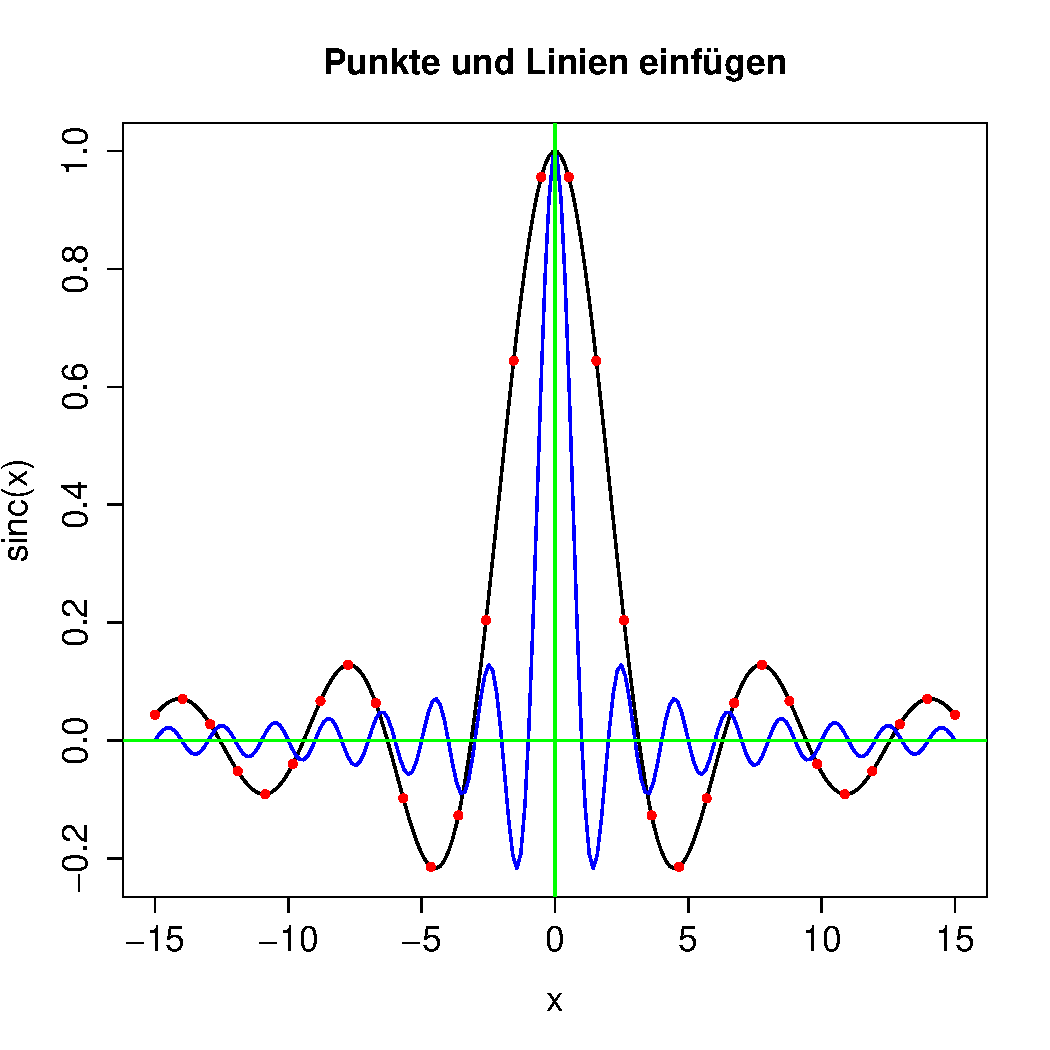
\includegraphics[width=8cm]{addPointsLines}
\vspace*{-1em}
\caption{Einfügen von Diagrammelementen: Punkte und Linien}
\label{fig:addPointsLines}
\end{figure}

\index{Grafik!Gitter}
\begin{lstlisting}
grid(nx=NULL, ny=nx)
\end{lstlisting}

Die Argumente \lstinline!nx! und \lstinline!ny! von\index[func]{grid()@\lstinline{grid()}} \lstinline!grid()! bestimmen, wie viele Elemente in das einzufügende Gitter senkrecht zur $x$- und $y$-Achse eingezeichnet werden. Auf \lstinline!NULL! gesetzt bildet das Gitter die Fortsetzung der Wertemarkierungen der zugehörigen Achse. Sollen keine Gitterelemente senkrecht zu einer Achse gezeichnet werden, ist das entsprechende Argument auf \lstinline!NA! zu setzen. Für quadratische Gitterfelder muss beim Erstellen des Diagramms z.\,B.\ mit \lstinline!plot()! das\index{Grafik!Seitenverhältnis} Seitenverhältnis mit dem Argument \lstinline!asp=1! kontrolliert werden.

Im folgenden Diagramm wird das Ergebnis einer Regression grafisch veranschaulicht, insbesondere die Residuen als Differenz der tatsächlichen zu den vorhergesagten Werten (Abb.\ \ref{fig:addGridArrows}).
\begin{lstlisting}
> height <- rnorm(20, 175, 7)                       # Prädiktor
> weight <- 0.5*height + 10 + rnorm(20, 0, 4)       # Kriterium
> fit    <- lm(weight ~ height)                     # Regression
> pred   <- fitted(fit)                             # Vorhersage
> plot(weight ~ height, asp=1, col="blue", pch=16,
+      main="Gitter, Segmente und Pfeile einfügen")

> abline(fit, lwd=2)                                # Regressionsgerade
> grid(lwd=2, col="darkgray")
\end{lstlisting}

\index{Grafik!Liniensegmente}
Einzelne Liniensegmente können mit\index[func]{segments()@\lstinline{segments()}} \lstinline!segments()! eingezeichnet werden. Dazu werden in der Funktion die $(x, y)$-Koordinaten der Endpunkte der Segmente angegeben.
\begin{lstlisting}
segments(x0=<<x Start>>, y0=<<y Start>>, x1=<<x Ziel>>, y1=<<y Ziel>>)
\end{lstlisting}

Unter \lstinline!x0! und \lstinline!y0! sind die Koordinaten des Startpunkts zu nennen, von dem ausgehend das Segment gezeichnet wird. Unter \lstinline!x1! und \lstinline!y1! wird der Zielpunkt des Segments mit seinen Koordinaten angegeben. Wenn mehrere Linien zu zeichnen sind, lassen sich die Koordinaten auch als Vektoren eingeben.
\begin{lstlisting}
# Differenz Vorhersage-Kriterium (Residuen)
> segments(x0=height, y0=pred, x1=height, y1=weight, col="gray")
\end{lstlisting}

\index{Grafik!Pfeile}
Ähnlich wie Liniensegmente können auch Pfeile mit\index[func]{arrows()@\lstinline{arrows()}} \lstinline!arrows()! in ein Diagramm eingezeichnet werden.
\begin{lstlisting}
arrows(x0=<<x Start>>, y0=<<y Start>>, x1=<<x Ziel>>, y1=<<y Ziel>>,
       length=0.25, angle=30, code=2)
\end{lstlisting}

Unter \lstinline!x0! und \lstinline!y0! werden die Koordinaten des Startpunkts eingegeben, von dem ausgehend der Pfeil gezeichnet wird. Unter \lstinline!x1! und \lstinline!y1! wird der Zielpunkt des Pfeils mit seinen Koordinaten angegeben. Wenn mehrere Pfeile eingefügt werden sollen, können die Koordinaten auch als Vektoren eingegeben werden. Das Argument \lstinline!length! kontrolliert die Länge der Pfeilspitzen in der Einheit inch, ihr Winkel wird über \lstinline!angle! in Grad festgelegt. In der Voreinstellung \lstinline!code=2! wird eine Pfeilspitze am Zielpunkt eingezeichnet, mit \lstinline!code=1! am Startpunkt, mit \lstinline!code=3! an beiden Enden (Abb.\ \ref{fig:addGridArrows}).
\begin{lstlisting}
> arrows(x0=c(height[1]-3,   height[3]),
+        y0=c(weight[1],     weight[3]+3),
+        x1=c(height[1]-0.5, height[3]),
+        y1=c(weight[1],     weight[3]+0.5), col="red", lwd=2)

> arrows(x0=height[4] + 0.1*(height[8] - height[4]),
+        y0=weight[4] + 0.1*(weight[8] - weight[4]),
+        x1=height[4] + 0.9*(height[8] - height[4]),
+        y1=weight[4] + 0.9*(weight[8] - weight[4]),
+        code=3, col="red", lwd=2)
\end{lstlisting}

\begin{figure}[ht]
\centering
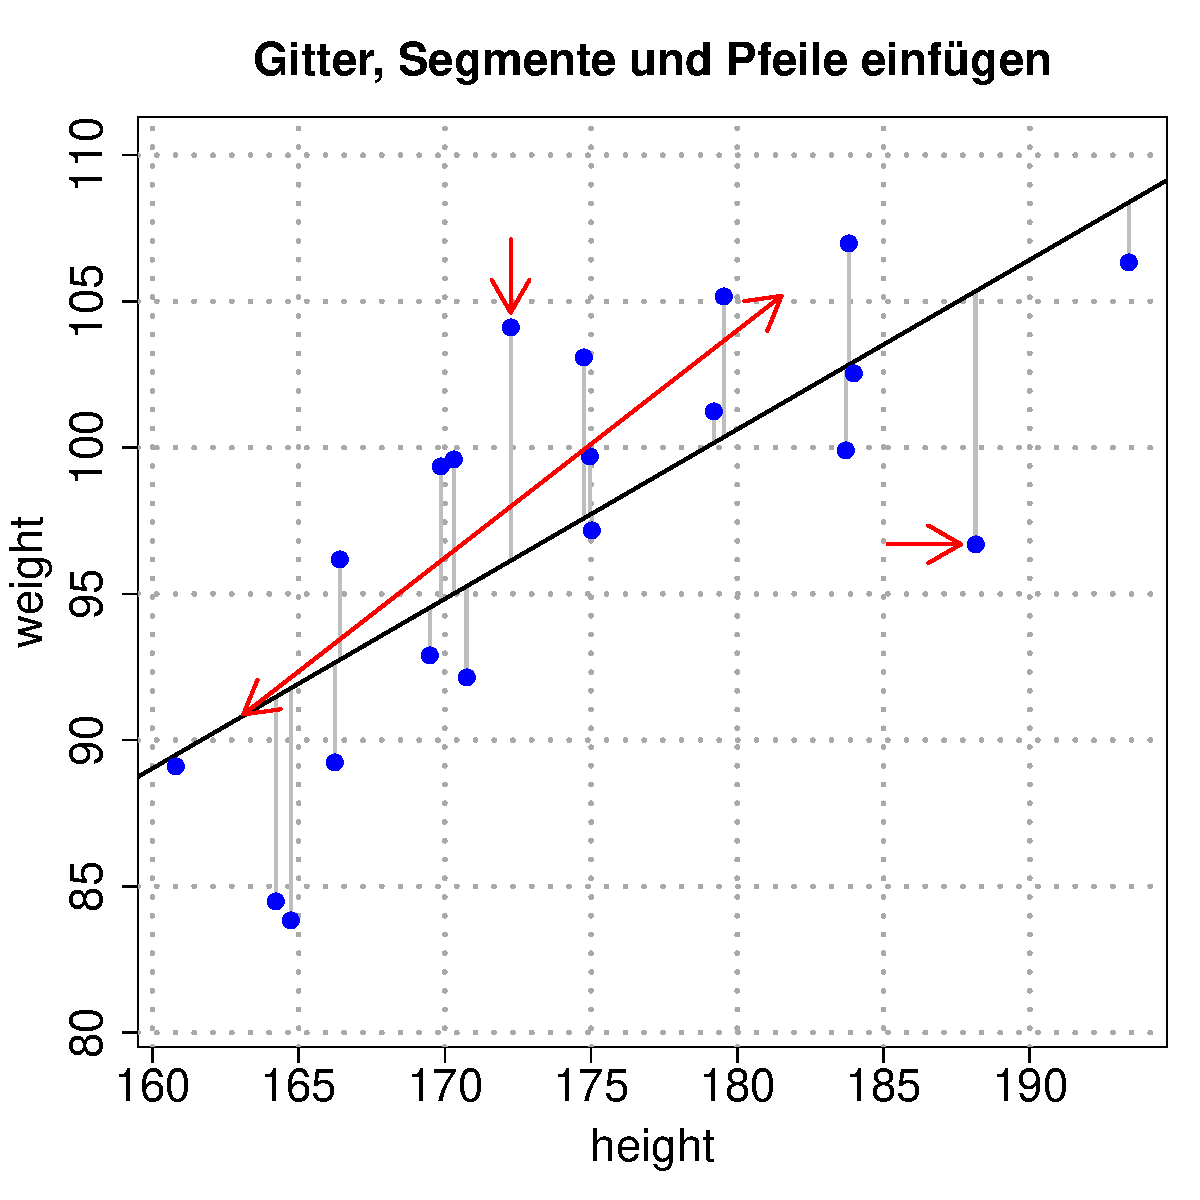
\includegraphics[width=8cm]{addGridArrows}
\vspace*{-1em}
\caption{Einfügen von Diagrammelementen: Gitter, Liniensegmente und Pfeile}
\label{fig:addGridArrows}
\end{figure}

%%%%%%%%%%%%%%%%%%%%%%%%%%%%%%%%%%%%%%%%%%%%%%%%%%%%%%%%%%%%%%%%%%
%%%%%%%%%%%%%%%%%%%%%%%%%%%%%%%%%%%%%%%%%%%%%%%%%%%%%%%%%%%%%%%%%%
\subsection{Polygone}
%%%%%%%%%%%%%%%%%%%%%%%%%%%%%%%%%%%%%%%%%%%%%%%%%%%%%%%%%%%%%%%%%%
%%%%%%%%%%%%%%%%%%%%%%%%%%%%%%%%%%%%%%%%%%%%%%%%%%%%%%%%%%%%%%%%%%

\index{Grafik!Rahmen}
Einem Diagramm kann mit\index[func]{box()@\lstinline{box()}} \lstinline!box(which="<<Region>>")! an verschiedenen Stellen ein rechteckiger Rahmen hinzugefügt werden. Das Argument \lstinline!which! bestimmt, ob der Rahmen um die Plot-Region (\lstinline!"plot"!) oder das gesamte Diagramm (\lstinline!"figure"!) gezeichnet werden soll. Andere mögliche Werte sind \lstinline!"inner"! und \lstinline!"outer"!, die in der Voreinstellung identische Ergebnisse zu \lstinline!"figure"! erzielen und sich nur bei geänderten Seitenrändern anders verhalten.

\index{Grafik!Rechtecke}
\index[func]{rect()@\lstinline{rect()}}
\lstinline!rect()! erzeugt beliebig dimensionierte Rechtecke, die sich in der Plot-Region frei plazieren lassen.
\begin{lstlisting}
rect( xleft=<<x-Koord. links>>, ybottom=<<y-Koord. unten>>,
     xright=<<x-Koord. rechts>>,   ytop=<<y-Koord. oben>>, border=NULL)
\end{lstlisting}

Die Argumente \lstinline!xleft!, \lstinline!ybottom!, \lstinline!xright! und \lstinline!ytop! akzeptieren Vektoren, die jeweils die Koordinaten der linken ($x$), unteren ($y$), rechten ($x$) und oberen Seiten ($y$) der zu zeichnenden Rechtecke enthalten. Soll kein Rahmen um ein Rechteck gezogen werden, ist \lstinline!border=NA! zu setzen (Abb.\ \ref{fig:rect}; \citeNP{Hoffman2000}).
\begin{lstlisting}
> n   <- 7                               # Anzahl an Zeilen und Spalten
> len <- 1/n                             # Kantenlänge eines Quadrats

# Farbverlauf im RGB Farbsystem erstellen (Blau-Anteil ist überall 0)
> colsR <- rep(seq(0.9, 0.2, length.out=n), each=n)   # Rot-Anteil
> colsG <- rep(seq(0.9, 0.2, length.out=n), times=n)  # Grün-Anteil
> cols  <- rgb(colsR, colsG, 0)                       # Farben in RGB

# Koordinaten der Quadrate festlegen
> xLeft  <- rep(seq(0,   1-len, by=len), times=n)     # x-Koord. links
> yBot   <- rep(seq(0,   1-len, by=len), each=n)      # y-Koord. unten
> xRight <- rep(seq(len, 1,     by=len), times=n)     # x-Koord. rechts
> yTop   <- rep(seq(len, 1,     by=len), each=n)      # y-Koord. oben

# zunächst ein leeres Diagramm erzeugen, dann Rechtecke einzeichnen
> par(oma=c(1, 1, 1, 1), mar=c(0, 0, 1, 0))            # Ränder ändern
> plot(c(0,1), c(0,1), axes=FALSE, type="n", asp=1, main="Farbverlauf")
> rect(xLeft, yBot, xRight, yTop, border=NA, col=cols)

# zwei Quadrate mit ihren hexadezimalen Farbwerten beschriften
> idx   <- c(10, 27)
> xText <- xLeft[idx] + (xRight[idx] - xLeft[idx])/2
> yText <- yBot[idx]  + (yTop[idx]   -  yBot[idx])/2
> text(xText, yText, labels=cols[idx])

# für zweites Diagramm Farben in zufällige Reihenfolge bringen
> shuffled <- sample(seq(along=cols), length(cols), replace=FALSE)
> idxS     <- c(which(shuffled == idx[1]), which(shuffled == idx[2]))
> plot(c(0, 1), c(0, 1), axes=FALSE, type="n", asp=1,
+       main="Dieselben Farben zufällig angeordnet")

> rect(xLeft, yBot, xRight, yTop, border=NA, col=cols[shuffled])

# die zwei Quadrate mit ihren hexadezimalen Farbwerten beschriften
> xTextS <- xLeft[idxS] + (xRight[idxS] - xLeft[idxS])/2
> yTextS <- yBot[idxS]  + (yTop[idxS]   -  yBot[idxS])/2
> text(xTextS, yTextS, labels=cols[idx])
\end{lstlisting}

\begin{figure}[ht]
\centering
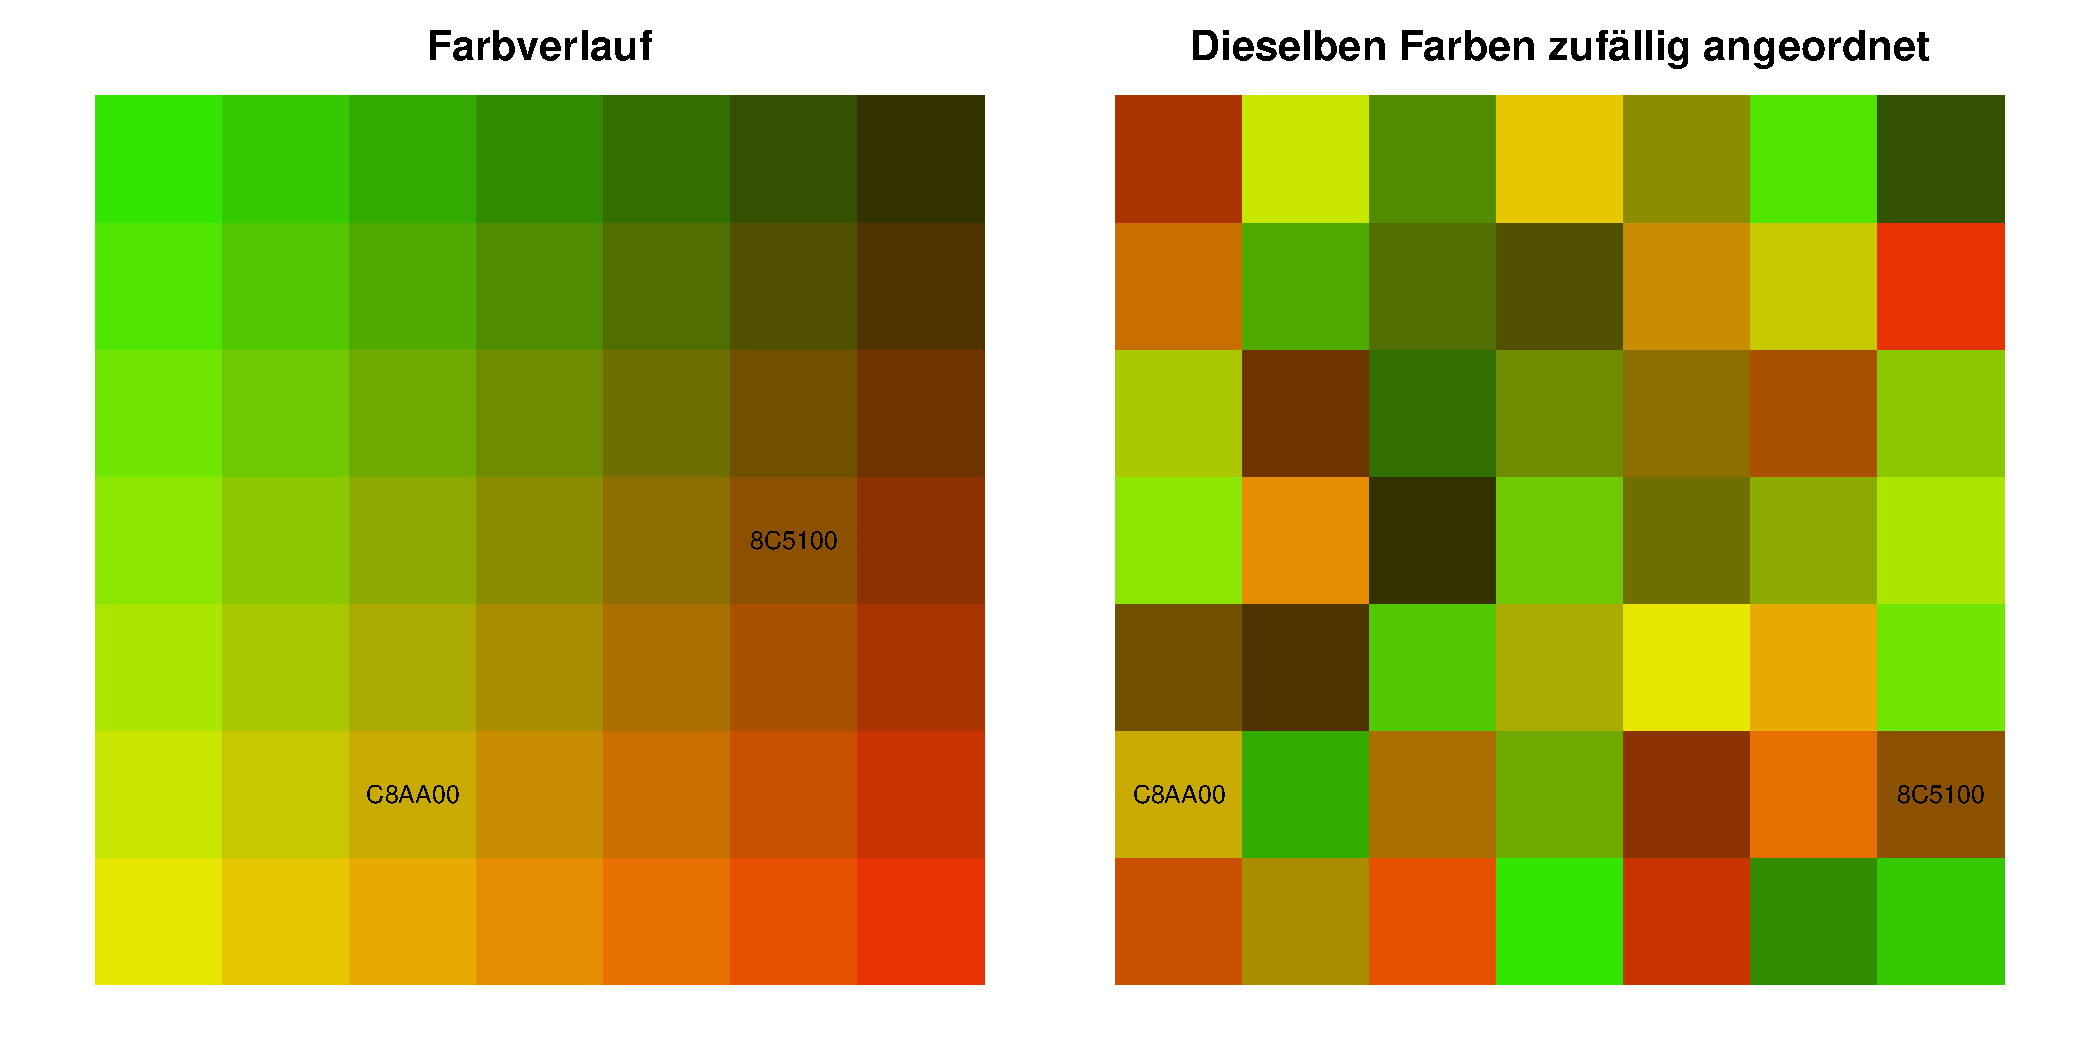
\includegraphics[width=12.5cm]{rect}
\vspace*{-1em}
\caption{Mit \lstinline!rect()! erzeugte Rechtecke zur Veranschaulichung eines Farbphänomens: Beide Grafiken sind aus denselben Quadraten zusammengesetzt, die jedoch -- auch abgesehen vom Chevreul-Effekt links -- in den beiden Konfigurationen unterschiedlich aussehen. Zwei jeweils links und rechts identische Farben sind mit ihrem Hexadezimalwert bezeichnet}
\label{fig:rect}
\end{figure}

\index{Grafik!Polygone}
\index[func]{polygon()@\lstinline{polygon()}}
\lstinline!polygon()! erzeugt Vielecke beliebiger Gestalt, deren Eckpunkte über ihre jeweiligen $(x, y)$-Koordinaten zu definieren sind und in Form von Vektoren an \lstinline!x! und \lstinline!y! übergeben werden können. Das Polygon wird geschlossen, indem R den ersten und letzten Punkt miteinander verbindet.\footnote{Mit \index[func]{polypath()@\lstinline{polypath()}} \lstinline!polypath()! lassen sich auch Polygone mit sich selbst überschneidenden Kanten zeichnen.} Soll kein Rahmen gezogen werden, ist \lstinline!border=NA! zu setzen. Mittels eng gesetzter Eckpunkte lassen sich auch runde Formen durch Polygone approximieren.
\begin{lstlisting}
polygon(x=<<x-Koordinaten>>, y=<<y-Koordinaten>>, border=NULL)
\end{lstlisting}

Das folgende Beispiel illustriert die Beziehung zwischen der Fläche unter der Kurve der Dichtefunktion einer Normalverteilung und der Wahrscheinlichkeit von Intervallen, wie sie sich an der zugehörigen Verteilungsfunktion als Differenz der Funktionswerte der Intervallgrenzen ablesen lässt. Im Diagramm werden beide Funktionen gleichzeitig unter Verwendung unterschiedlicher $y$-Achsen dargestellt (Abb.\ \ref{fig:axisPolygon}).
\begin{lstlisting}
> mu    <- 0                         # Erwartungswert
> sigma <- 3                         # Streuung
> xLims <- c(mu-4*sigma, mu+4*sigma) # Grenzen x-Achse
> X     <- seq(xLims[1], xLims[2], length.out=100)      # x-Werte
> Y     <- dnorm(X, mu, sigma)       # Werte der Dichtefunktion
> selX  <- seq(mu-sigma, mu+sigma, length.out=100)      # [mu +- sigma]
> selY  <- dnorm(selX, mu, sigma)    # Werte im Intervall [mu +- sigma]
> cdf   <- pnorm(X, mu, sigma)       # Werte der Verteilungsfunktion

# Grafik leer mit breitem rechten Rand öffnen
> par(mar=c(5, 4, 4, 5))
> plot(X, Y, type="n", xlim=xLims-c(-2, 2), xlab=NA, ylab=NA,
+      main="Dichtefunktion und Verteilungsfunktion N(0, 3)")

# Rahmen, Fläche über Intervall [mu +- sigma] zeichnen
> box(which="plot", col="gray", lwd=2)
> polygon(c(selX, rev(selX)), c(selY, rep(-1, length(selX))),
+         border=NA, col="lightgray")

> lines(X, Y, lwd=2)                  # Dichtefunktion

# Verteilungsfunktion einzeichnen
> par(new=TRUE)            # folgendes Diagramm in bestehendes zeichnen
> plot(X, cdf, xlim=xLims-c(-2, 2), type="l", lwd=2, col="blue",
+      xlab="x", ylab=NA, axes=FALSE)

# Achsen und Hilfslinien einzeichnen
> axis(side=4, at=seq(0, 1, by=0.1), col="blue")
> segments(x0=c(mu-sigma, mu, mu+sigma),
+          y0=c(-1, -1, -1),
+          x1=c(      mu-sigma, mu, mu+sigma),
+          y1=c(pnorm(mu-sigma, mu,    sigma),
+               pnorm(mu,       mu,    sigma),
+               pnorm(mu+sigma, mu,    sigma)),
+          lwd=2, col=c("darkgreen", "red", "darkgreen"), lty=2)

> segments(x0=c(      mu-sigma, mu, mu+sigma),
+          y0=c(pnorm(mu-sigma, mu,    sigma),
+               pnorm(mu,       mu,    sigma),
+               pnorm(mu+sigma, mu,    sigma)),
+          x1=xLims[2]+10,
+          y1=c(pnorm(mu-sigma, mu,    sigma),
+               pnorm(mu,       mu,    sigma),
+               pnorm(mu+sigma, mu,    sigma)),
+          lwd=2, col=c("darkgreen", "red", "darkgreen"), lty=2)

> arrows(x0=c(mu-sigma+0.2, mu+sigma-0.2), y0=-0.02,
+        x1=c(mu-0.2,       mu+0.2),       y1=-0.02,
+        code=3, angle=90, length=0.05, lwd=2, col="darkgreen")

# zusätzliche Beschriftungen
> mtext(text="F(x)", side=4, line=3)
> rect(-8.5, 0.92, -5.5, 1.0, col="lightgray", border=NA)
> text(-7.2, 0.9, labels="Wahrscheinlichkeit")
> text(-7.1, 0.86, expression(des~~Intervalls~~group("[",
+      list(-sigma, sigma), "]")))

> text(mu-sigma/2, 0,    expression(sigma), col="darkgreen", cex=1.2)
> text(mu+sigma/2, 0,    expression(sigma), col="darkgreen", cex=1.2)
> text(mu+0.5,     0.02, expression(mu),    col="red",       cex=1.2)
\end{lstlisting}

\begin{figure}[ht]
\centering
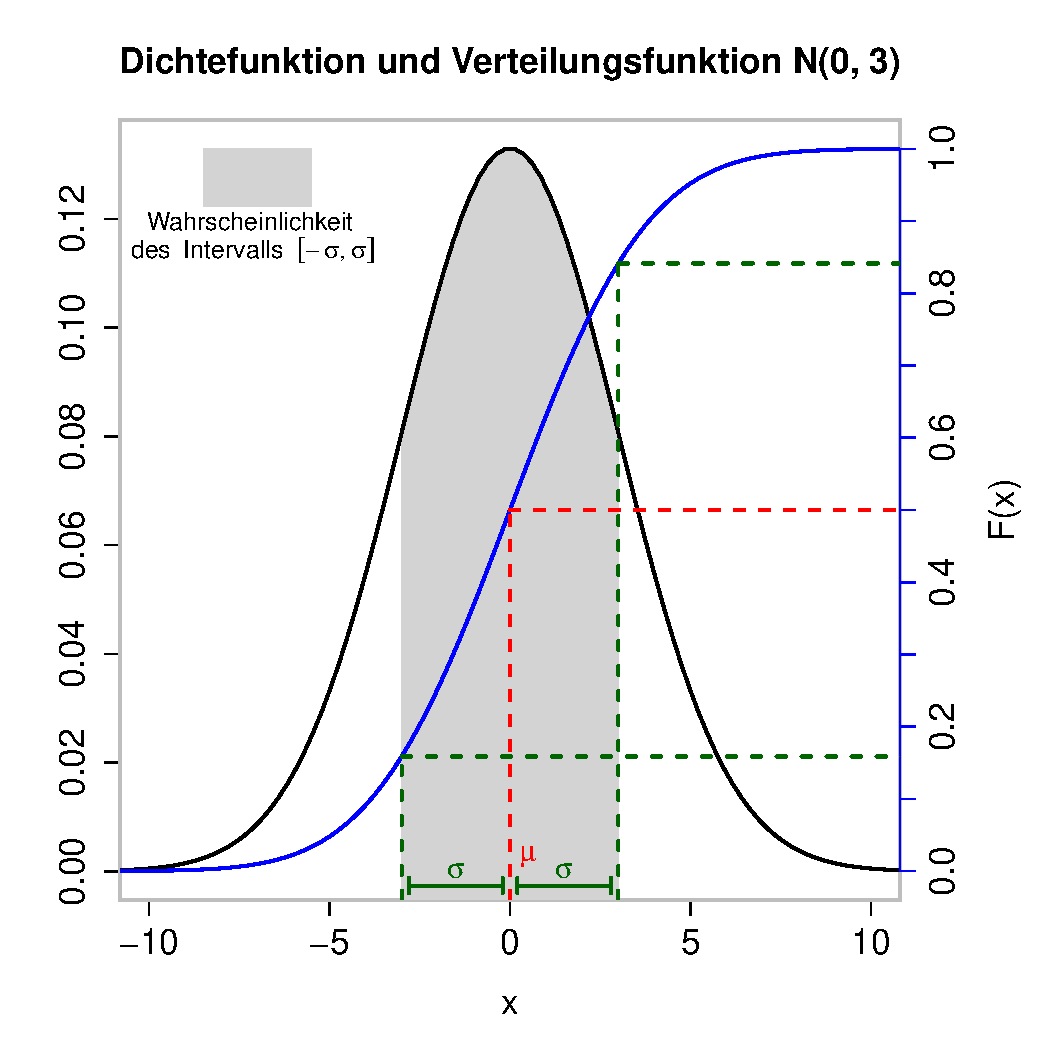
\includegraphics[width=8cm]{axisPolygon}
\vspace*{-1em}
\caption{Diagrammelemente einfügen: Rechtecke, Polygone, Achsen, Text und Symbole}
\label{fig:axisPolygon}
\end{figure}

%%%%%%%%%%%%%%%%%%%%%%%%%%%%%%%%%%%%%%%%%%%%%%%%%%%%%%%%%%%%%%%%%%
%%%%%%%%%%%%%%%%%%%%%%%%%%%%%%%%%%%%%%%%%%%%%%%%%%%%%%%%%%%%%%%%%%
\subsection{Funktionsgraphen}
%%%%%%%%%%%%%%%%%%%%%%%%%%%%%%%%%%%%%%%%%%%%%%%%%%%%%%%%%%%%%%%%%%
%%%%%%%%%%%%%%%%%%%%%%%%%%%%%%%%%%%%%%%%%%%%%%%%%%%%%%%%%%%%%%%%%%

\index{Grafik!Funktionsgraph}
\index[func]{curve()@\lstinline{curve()}}
\index{Funktionsgraph|see{Grafik}}
\begin{lstlisting}
curve(expr=<<Funktion>>, from=<<Zahl>>, to=<<Zahl>>, n=101, add=FALSE)
\end{lstlisting}

Die High-Level-Funktion \lstinline!curve()! dient dazu, Graphen von beliebigen Funktionen mit einer Veränderlichen zu erstellen. Dabei kann die darzustellende Funktion als Funktionsgleichung mit \lstinline!x! als Variable spezifiziert werden (z.\,B.\ \lstinline!dnorm(x, mean=1, sd=1)! oder \lstinline!x^2 + 10!). Hier wird also dieselbe Notation benutzt, wie um aus einem bestehenden Vektor \lstinline!x! einen neuen Vektor mit den Funktionswerten zu generieren. Als Kurzform lässt sich auch nur der Name einer Funktion angeben (z.\,B.\ \lstinline!dnorm!), die dann mit den Voreinstellungen für ihre Argumente aufgerufen wird. In welchem Wertebereich die Funktion ausgewertet werden soll, bestimmen die Argumente \lstinline!from! und \lstinline!to!. Dabei legt das Argument \lstinline!n! die Anzahl der Stützstellen fest, an wie vielen gleichabständigen Stellen in diesem Bereich also Funktionswerte bestimmt und eingezeichnet werden. Um den Funktionsgraphen dem aktuell aktiven device hinzuzufügen, ohne dessen Inhalte zu löschen, ist \lstinline!add=TRUE! zu setzen (Abb.\ \ref{fig:addGraphsText}). Als auf der Konsole unsichtbaren Rückgabewert liefert \lstinline!curve()! eine Liste mit den $(x, y)$-Koordinaten der gezeichneten Punkte.
\begin{lstlisting}
> mu    <- 0                   # Normalverteilung Erwartungswert
> sigma <- 2                   # theoretische Streuung
> curve(dnorm(x, mean=1, sd=1), from=-7, to=7, col="blue", lwd=2)
> curve((1/(sigma*sqrt(2*pi))) * exp(-0.5*(((x-mu)/sigma)^2)),
+       add=TRUE, lwd=2, lty=2)
\end{lstlisting}

%%%%%%%%%%%%%%%%%%%%%%%%%%%%%%%%%%%%%%%%%%%%%%%%%%%%%%%%%%%%%%%%%%
%%%%%%%%%%%%%%%%%%%%%%%%%%%%%%%%%%%%%%%%%%%%%%%%%%%%%%%%%%%%%%%%%%
\subsection{Text und mathematische Formeln}
%%%%%%%%%%%%%%%%%%%%%%%%%%%%%%%%%%%%%%%%%%%%%%%%%%%%%%%%%%%%%%%%%%
%%%%%%%%%%%%%%%%%%%%%%%%%%%%%%%%%%%%%%%%%%%%%%%%%%%%%%%%%%%%%%%%%%

\index{Grafik!Titel}
\index{Grafik!Beschriftung}
\index[func]{title()@\lstinline{title()}}
\begin{lstlisting}
title(main="<<Titel>>", sub="<<Untertitel>>")
\end{lstlisting}

Der Diagrammtitel lässt sich in High-Level-Grafikfunktionen meist über das Argument \lstinline!main="<<Name>>"!, ein Untertitel über \lstinline!sub="<<Name>>"! hinzufügen. Soll der Diagrammtitel nachträglich festgelegt werden, kann die separat aufzurufende Low-Level-Funktion \lstinline!title()! Verwendung finden, die ihrerseits \lstinline!main! und \lstinline!sub! als Argumente besitzt. Die Escape-Sequenz \lstinline!\n! dient innerhalb einer Zeichenkette als Symbol für den Zeilenwechsel (Abb.\ \ref{fig:addGraphsText}).
\begin{lstlisting}
> title(main="zwei Normalverteilungskurven", sub="Untertitel")
\end{lstlisting}

\index{Grafik!Legende}
\index[func]{legend()@\lstinline{legend()}}
Eine Legende zur Erläuterung der verwendeten Symbole erstellt \lstinline!legend()!.
\begin{lstlisting}
legend(x=<<x-Koordinate>>, y=<<y-Koordinate>>, legend="<<Text>>",
       col="<<Farben>>", lty=<<Linientypen>>, lwd=<<Linienstärken>>,
       pch=<<Symbole>>)
\end{lstlisting}

Die Legende wird entweder über die Angabe von $(x, y)$-Koordinaten für die Argumente \lstinline!x! und \lstinline!y! positioniert, oder durch Nennung eines der Schlüsselwörter \lstinline!"bottomright"!, \lstinline!"bottom"!, \lstinline!"bottomleft"!, \lstinline!"left"!, \lstinline!"topleft"!, \lstinline!"top"!, \lstinline!"topright"!, \lstinline!"right"! oder \lstinline!"center"! für \lstinline!x!. Der Legendentext selbst ist als Vektor von Zeichenketten an \lstinline!legend! zu übergeben, wobei jedes Element dieses Vektors einen Legendeneintrag definiert. Welches Aussehen dem Symbol neben einem Eintrag verliehen wird, kontrollieren die Argumente \lstinline!col! (Farbe), \lstinline!lty! (Linientyp), \lstinline!lwd! (Linienstärke) und \lstinline!pch! (Symbol, s.\ Abschn.\ \ref{sec:par}). Für diese Argumente ist jeweils ein Vektor derselben Länge wie \lstinline!legend! einzugeben, wobei \lstinline!NA! Einträge bedeuten, dass die definierte Eigenschaft nicht auf das zugehörige Legendensymbol zutrifft.

Sind in einem Diagramm etwa sowohl zwei Punkt-Reihen als auch zwei Linien enthalten, würde die Kombination von \lstinline!pch=c(19, 20, NA, NA)! und \lstinline!lty=c(NA, NA, 1, 2)! bewirken, dass die ersten beiden Legendeneinträge mit den Symbolen $19$ und $20$ dargestellt werden, die letzten beiden Einträge mit den Linientypen $1$ und $2$.
\begin{lstlisting}
> legend(x="topleft", legend=c("N(1, 1)", "N(0, 2)"),
+        col=c("blue", "black"), lty=c(1, 2))
\end{lstlisting}

\index{Grafik!Text}
\index{Grafik!Beschriftung}
Mit\index[func]{text()@\lstinline{text()}} \lstinline!text()! lässt sich allgemein Text an beliebiger Stelle in die Plot-Region eines Diagramms einfügen.
\begin{lstlisting}
text(x=<<x-Koordinaten>>, y=<<y-Koordinaten>>, adj=<<Positionskorrektur>>,
     labels="<<Name>>", srt=<<Rotationswinkel>>)
\end{lstlisting}

Zunächst sind mit den Argumenten \lstinline!x! und \lstinline!y! die Koordinaten des Texts festzulegen. Sollen mehrere Textelemente gleichzeitig eingefügt werden, sind hier Vektoren zu übergeben. In der Voreinstellung beziehen sich die Koordinaten auf den Mittelpunkt des Texts, was jedoch über \lstinline!adj! veränderbar ist: Durch einen Vektor mit zwei Elementen im Intervall $[0, 1]$ kann der Bezugspunkt der $(x, y)$-Koordinaten vom linken unteren Textrand (\lstinline!c(0, 0)!) zum rechten oberen Textrand (\lstinline!c(1, 1!)) verschoben werden, Voreinstellung ist \lstinline!c(0.5, 0.5)! für die Textmitte. Die Texte selbst müssen dem Argument \lstinline!labels! in Form eines Vektors von Zeichenketten übergeben werden. Das Argument \lstinline!srt! erwartet eine Winkelangabe in Grad und erlaubt es, den Text um den mit \lstinline!adj! definierten Drehpunkt zu rotieren.
\begin{lstlisting}
> text(x=3.6,  y=0.35, labels="Normalverteilung\nN(1, 1)")
> text(x=-3.5, y=0.1,  labels="N(0, 2)")
\end{lstlisting}

\index{Grafik!Text}
\index{Grafik!Beschriftung}
Sollen Textelemente nicht innerhalb der Plot-Region, sondern an deren äußere Ränder geschrieben werden, ist\index[func]{mtext()@\lstinline{mtext()}} \lstinline!mtext()! hilfreich.
\begin{lstlisting}
mtext(text="<<Name>>", side=<<Nummer>>, line=<<Nummer>>)
\end{lstlisting}

Während das Argument \lstinline!text! die darzustellenden Texte in Form eines Vektors von Zeichenketten akzeptiert, bestimmt \lstinline!side! mit einem Vektor der Zahlen $1$--$4$, an welcher Seite der Text erscheinen soll. Die \lstinline!1! steht dabei für unten, \lstinline!2! für links, \lstinline!3! für oben (Voreinstellung) und \lstinline!4! für rechts. Die Orientierung des Texts ist immer parallel zum Rand, an dem der Text steht. Das Argument \lstinline!line! legt in Form eines Vielfachen der Linienhöhe fest, wie weit außen der Text dargestellt wird, wobei $0$ dem Rand der Plot-Region entspricht.
\begin{lstlisting}
> mtext(text="Wahrscheinlichkeitsdichte", side=3)
\end{lstlisting}

\index{Grafik!mathematische Formeln}
\index{Grafik!Symbole}
\index[func]{expression()@\lstinline{expression()}}
In allen Funktionen zum Einfügen von Text können mit Hilfe einer an das Textsatzsystem \LaTeX{} angelehnten Syntax auch jedwede Art von Symbolen (griechische Buchstaben, mathematische Sonderzeichen, etc.) und mathematische Formeln definiert werden \cite{Ligges2002}. Zu diesem Zweck wird eine Formel in Textform an \lstinline!expression(<<Ausdruck>>)! übergeben und das Ergebnis in den Funktionen zum Einfügen von Text eingesetzt. \lstinline!<<Ausdruck>>! enthält dabei etwa Text (ohne Anführungszeichen), lateinische Umschreibungen griechischer Buchstaben (\lstinline!theta!), Summenzeichen (\lstinline!sum(x[i], i==1, n)!) Brüche (\lstinline!frac(<<Zähler>>, <<Nenner>>)!) oder Wurzelsymbole (\lstinline!sqrt(<<Radikand>>, <<Wurzelexponent>>)!). Zeilenumbrüche mit der \lstinline!\n! Escape-Sequenz sind dagegen nicht möglich -- stattdessen müssen mehrere Zeilen durch mehrere \lstinline!text(x, y, expression())! Befehle mit entsprechend unterschiedlichen Koordinaten realisiert werden. Eine Einführung in die Verwendung enthält die Hilfe-Seite \lstinline!?plotmath!, weitere Veranschaulichungen zeigt \lstinline!demo(plotmath)!.
\begin{lstlisting}
> text(-4, 0.3, expression(frac(1, sigma*sqrt(2*pi)) ~~
+                         exp * bgroup("(", -frac(1, 2) ~~
+                         bgroup("(", frac(x-mu, sigma), ")")^2, ")")))
\end{lstlisting}

\begin{figure}[ht]
\centering
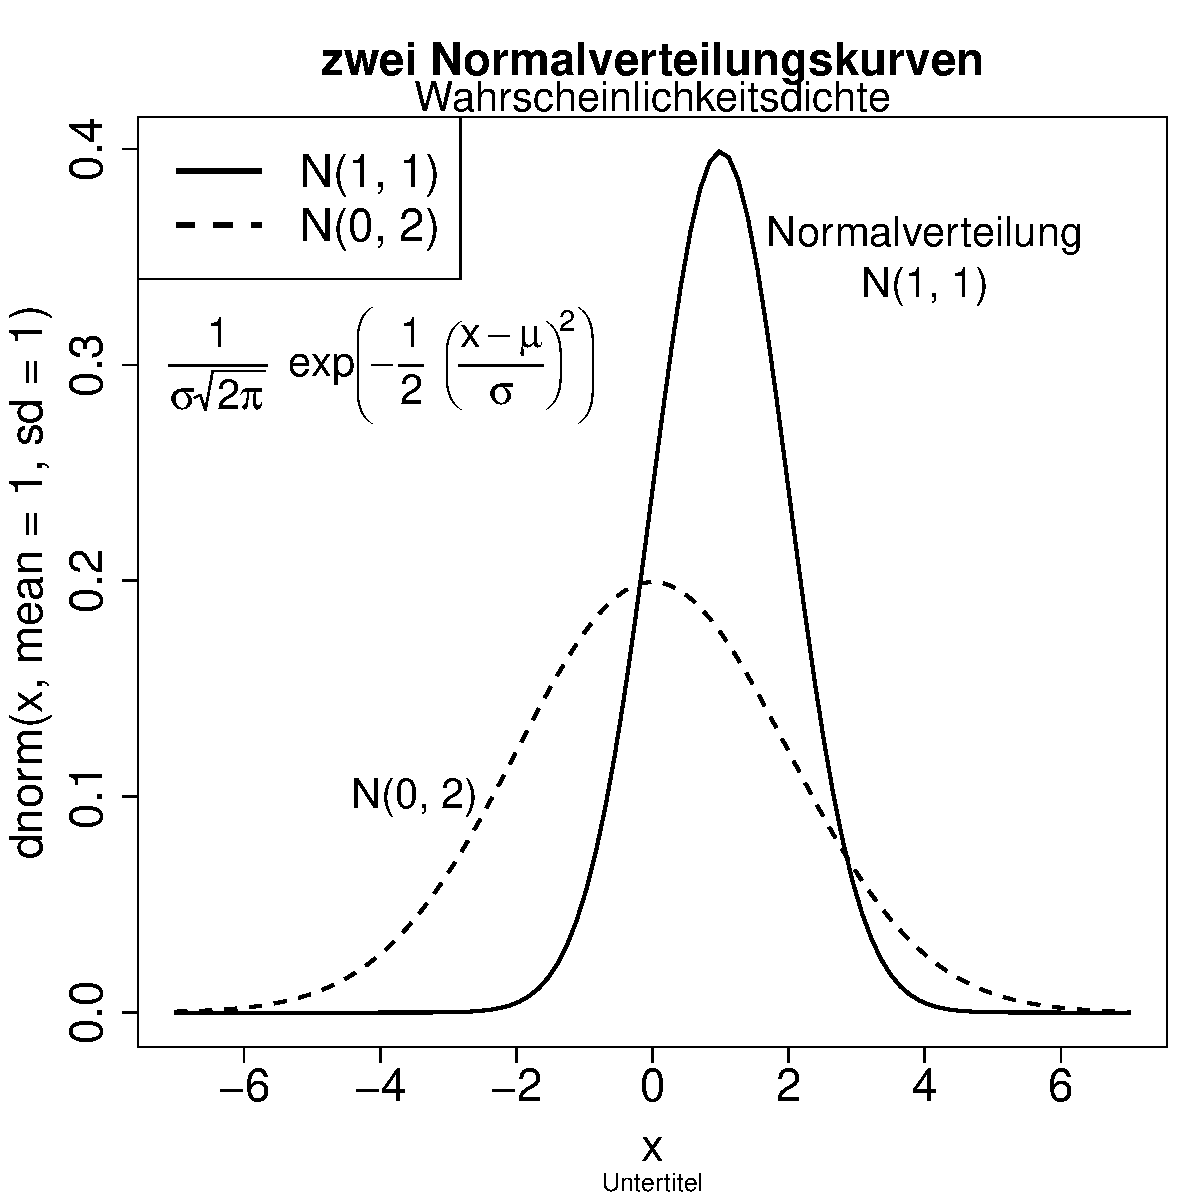
\includegraphics[width=8cm]{addGraphsText}
\vspace*{-0.5em}
\caption{Diagrammelemente einfügen: Funktionsgraphen, Text, Legende und mathematische Formeln}
\label{fig:addGraphsText}
\end{figure}

%%%%%%%%%%%%%%%%%%%%%%%%%%%%%%%%%%%%%%%%%%%%%%%%%%%%%%%%%%%%%%%%%%
%%%%%%%%%%%%%%%%%%%%%%%%%%%%%%%%%%%%%%%%%%%%%%%%%%%%%%%%%%%%%%%%%%
\subsection{Achsen}
\label{sec:axis}
%%%%%%%%%%%%%%%%%%%%%%%%%%%%%%%%%%%%%%%%%%%%%%%%%%%%%%%%%%%%%%%%%%
%%%%%%%%%%%%%%%%%%%%%%%%%%%%%%%%%%%%%%%%%%%%%%%%%%%%%%%%%%%%%%%%%%

\index{Grafik!Achsen}
Ob durch die Darstellung von Datenpunkten in einem Diagramm automatisch auch Achsen generiert werden, kontrollieren in High-Level-Grafikfunktionen die Argumente \lstinline!xaxt! für die $x$-Achse, \lstinline!yaxt! für die $y$-Achse und \lstinline!axes! für beide Achsen gleichzeitig. Während für \lstinline!xaxt! und \lstinline!yaxt! der Wert \lstinline!"n"! übergeben werden muss, um die Ausgabe der entsprechenden Achse zu unterdrücken, akzeptiert \lstinline!axes! dafür den Wert \lstinline!FALSE!\@.

\index{Grafik!Beschriftung}
Für eine feinere Kontrolle über den Wertebereich sowie über Aussehen und Lage der Wertemarkierungen der Achsen empfiehlt es sich, ihre automatische Generierung zunächst mit \lstinline!axes=FALSE! zu unterdrücken. Nachdem das Diagramm erstellt wurde, können dann mit dem Befehl\index[func]{axis()@\lstinline{axis()}} \lstinline!axis()! samt seiner Argumente zur Formatierung und Positionierung Achsen hinzugefügt werden (Abb.\ \ref{fig:axisPolygon}, \ref{fig:axis}).
\begin{lstlisting}
axis(side=<<Nummer>>, at=<<Markierungen>>,
     labels="<<Wertebeschriftungen>>", pos=<<Position>>)
\end{lstlisting}

Achsen lassen sich an allen Diagrammseiten darstellen, was über das Argument \lstinline!side! kontrolliert wird. Mögliche Werte sind \lstinline!1! (unten, $x$-Achse), \lstinline!2! (links, $y$-Achse), \lstinline!3! (oben, alternative $x$-Achse) und \lstinline!4! (rechts, alternative $y$-Achse). Die Wertemarkierungen der Achse lassen sich über \lstinline!at! in Form eines Vektors festlegen. Das Argument \lstinline!labels! bestimmt die Beschriftung dieser Markierungen und erwartet einen numerischen Vektor oder einen Vektor von Zeichenketten. Die Orientierung dieser Markierungen legt das Argument \lstinline!las! von \lstinline!par()! fest. Soll die Position der Achse nicht an den Rändern der Plot-Region liegen, kann sie auch in Form einer Koordinate über das Argument \lstinline!pos! definiert werden. Ist die Achse eine horizontale (\lstinline!side=1! oder \lstinline!3!), wird der Wert für \lstinline!pos! als $y$-Koordinate der Achse interpretiert, andernfalls (\lstinline!side=2! oder \lstinline!4!) als deren $x$-Koordinate.
\begin{lstlisting}
> vec <- seq(from=-2*pi, to=2*pi, length.out=200)
> mat <- cbind(sin(vec), cos(vec), tan(vec))
> mat <- ifelse(abs(mat) > 2, NA, mat)        # Werte > 2 auf NA setzen
> matplot(vec, mat, lwd=2, lty=c(1, 2, 4), col=c(12, 14, 17), type="l",
+         xaxt="n", xlab=NA, ylab=NA,
+         main="Trigonometrische Funktionen")

> xTicks  <- seq(from=-2*pi, to=2*pi, by=pi/2)
> xLabels <- c("-2*pi", "-3*pi/2", "-pi", "-pi/2", "0", "pi/2", "pi",
+              "3*pi/2", "2*pi")

> axis(side=1, at=xTicks, labels=xLabels)
> abline(h=c(-1, 0, 1), v=seq(from=-3*pi/2, to=3*pi/2, by=pi/2),
+        col="gray", lty=3, lwd=2)

> abline(h=0, v=0, lwd=2)
> legend(x="bottomleft", legend=c("sin(x)", "cos(x)", "tan(x)"),
+        lty=c(1, 2, 4), col=c(12, 14, 17))
\end{lstlisting}

\begin{figure}[ht]
\centering
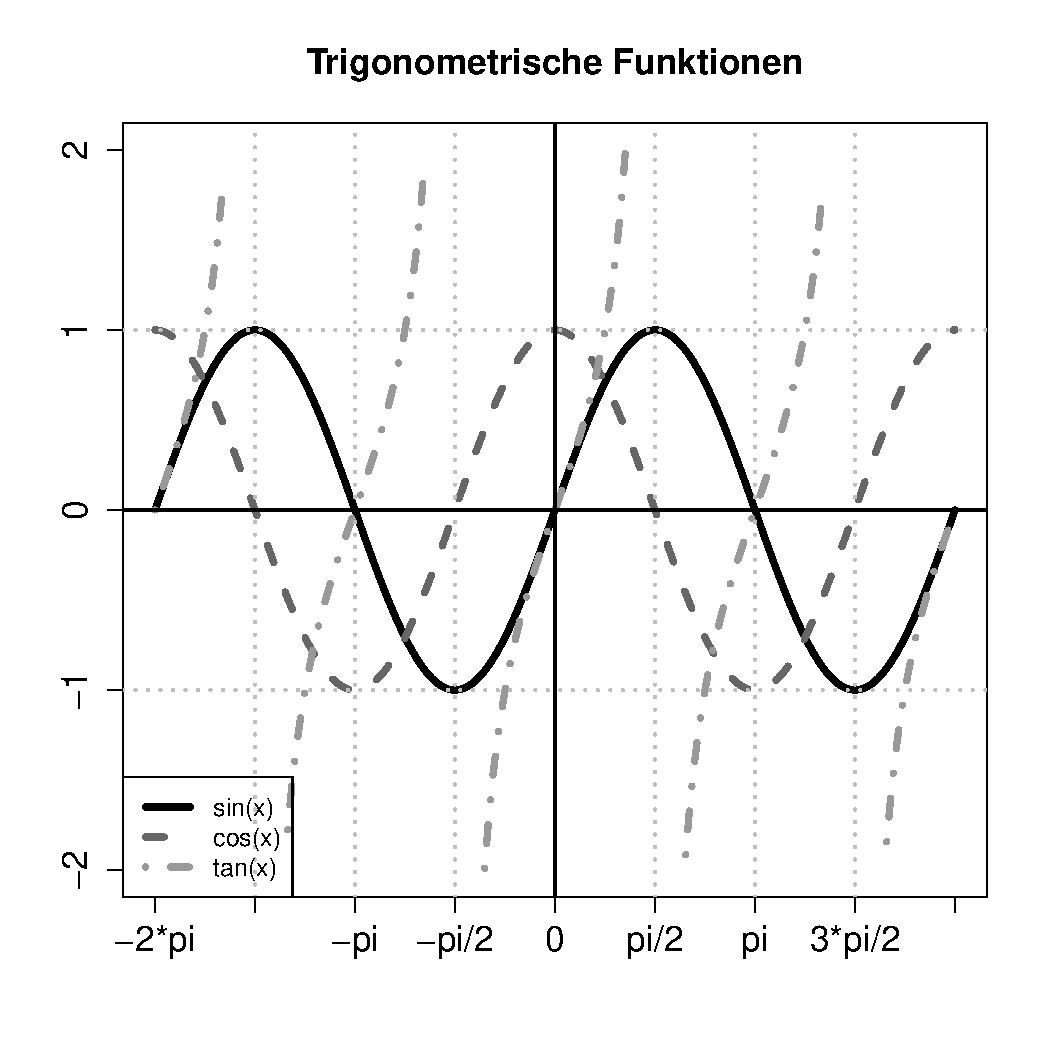
\includegraphics[width=8cm]{axis}
\vspace*{-1em}
\caption{Diagrammachsen mit \lstinline!axis()! anpassen}
\label{fig:axis}
\end{figure}

%%%%%%%%%%%%%%%%%%%%%%%%%%%%%%%%%%%%%%%%%%%%%%%%%%%%%%%%%%%%%%%%%%
%%%%%%%%%%%%%%%%%%%%%%%%%%%%%%%%%%%%%%%%%%%%%%%%%%%%%%%%%%%%%%%%%%
\subsection{Fehlerbalken}
%%%%%%%%%%%%%%%%%%%%%%%%%%%%%%%%%%%%%%%%%%%%%%%%%%%%%%%%%%%%%%%%%%
%%%%%%%%%%%%%%%%%%%%%%%%%%%%%%%%%%%%%%%%%%%%%%%%%%%%%%%%%%%%%%%%%%

\index{Grafik!Fehlerbalken}
\index{Fehlerbalken|see{Grafik}}
Fehlerbalken werden zusätzlich zu Kennwerten von Variablen vor allem in Punktdiagrammen eingezeichnet, um die Variabilität der Daten auszudrücken. Als Maß der Variabilität kann dabei u.\,a.\ die Breite eines statistischen Konfidenzintervalls für einen Parameter (z.\,B.\ den Erwartungswert) oder ein deskriptives Maß wie die Streuung verwendet werden.\footnote{Für Konfidenzellipsen als Maß für die Variabilität zweidimensionaler Daten vgl.\ Abschn.\ \ref{sec:distr2var}.}

Das Paket\index[pack]{DescTools@\lstinline{DescTools}} \lstinline!DescTools! enthält die Funktion\index[func]{ErrBars()@\lstinline{ErrBars()}} \lstinline!ErrBars()!, die Fehlerbalken einem bestehenden Diagramm hinzufügt. Das vertikale Zentrum der Fehlerbalken wird als Punkt gezeichnet, so dass es nicht unbedingt notwendig ist, zusätzlich Punkte zur Veranschaulichung des Parameters zu zeichnen, dessen Variabilität über einen Fehlerbalken dargestellt wird (Abb.\ \ref{fig:errorbars}).
\begin{lstlisting}
ErrBars(from=<<y-Koordinate unten>>, to=<<y-Koordinate oben>>,
        pos=<<x-Koordinate>>, horiz=FALSE)
\end{lstlisting}

Unter \lstinline!from! und \lstinline!to! werden die $y$-Koordinaten der unteren bzw.\ oberen Grenzen der Fehlerbalken definiert. Für \lstinline!pos! sind die $x$-Koordinaten der Fehlerbalken anzugeben.  Mit \lstinline!horiz! wird definiert, ob die Balken vertikal (Voreinstellung \lstinline!FALSE!) oder horizontal (\lstinline!TRUE!) zu zeichnen sind. Die Funktion verfügt über weitere Optionen zur Formatierung der Fehlerbalken bzgl.\ ihrer Farbe, Linienstärke, etc.
\begin{lstlisting}
# Simulation von Messwerten in 4 Gruppen ohne Gruppeneffekt
> Nj <- c(15, 20, 18, 22)                        # Gruppengrößen
> P  <- length(Nj)                               # Anzahl Gruppen
> DV <- rnorm(sum(Nj), rep(c(30, 20, 25, 15), Nj), 6)          # Daten
> IV <- factor(rep(1:P, Nj))                     # Gruppenzugehörigkeit
> Mj <- tapply(DV, IV, mean)                     # Gruppenmittel
> Sj <- tapply(DV, IV, sd)                       # Gruppenstreuungen

# halbe Breite 95% t-Konfidenzintervalle für Erwartungswerte
> ciWidths <- qt(0.975, Nj-1) * Sj/sqrt(Nj)

# Punktdiagramm getrennt nach Gruppen
> stripchart(DV ~ IV, method="jitter", xaxt="n", xlab="Gruppe",
+            ylim=c(0, 40), main="Rohdaten & Konfidenzintervalle",
+            col="darkgray", pch=16, vert=TRUE)

> library(DescTools)                             # für ErrBars()
> ErrBars(from=Mj-ciWidths, to=Mj+ciWidths, pos=1:P, length=0.1,
+         col="blue", col.pch="blue", lwd=2, pch=19)

> axis(side=1, at=1:P, labels=LETTERS[1:P])      # Gruppenbezeichnungen
\end{lstlisting}

Es können auch simultan Fehlerbalken für mehrere Gruppen dargestellt werden, die ähnlich einem gruppierten Säulendiagramm aufgebaut sind. Dabei wird die Gruppierung durch die Wahl der $x$-Koordinaten kontrolliert. Hier soll die Streuung die Länge der Fehlerbalken bestimmen.
\begin{lstlisting}
> Mj1  <- c(2, 3, 6, 3, 5)                       # Mittelwerte Gruppe 1
> Sj1  <- c(1.7, 1.8, 1.7, 1.9, 1.8)             # Streuungen Gruppe 1
> Mj2  <- c(4, 3, 2, 1, 3)                       # Mittelwerte Gruppe 2
> Sj2  <- c(1.4, 1.7, 1.7, 1.3, 1.5)             # Streuungen Gruppe 2
> Q    <- length(Mj1)                            # Anzahl Mittelwerte
> xOff <- 0.1        # horizontaler offset zwischen Werten einer Gruppe

# Mittelwerte
> plot(c((1:Q)-xOff, (1:Q)+xOff), c(Mj1, Mj2), pch=19,
+      main="Mittelwerte & SDs im 5x2 Design",
+      xlab="Faktor A", ylab="Mittelwert",
+      col=rep(c("blue", "red"), each=5), ylim=c(0, 8))

# Fehlerbalken
> ErrBars(from=c(Mj1, Mj2) - c(Sj1, Sj2),
+           to=c(Mj1, Mj2) + c(Sj1, Sj2),
+         pos=c((1:Q)-xOff, (1:Q)+xOff), lty=rep(1:2, each=Q),
+         col=rep(c("blue", "red"), each=Q),
+         col.pch=rep(c("blue", "red"), each=Q), pch=19)

> legend(x="topleft", legend=c("B-1", "B-2"), pch=c(19, 19),
+        col=c("blue", "red"))
\end{lstlisting}

\begin{figure}[ht]
\centering
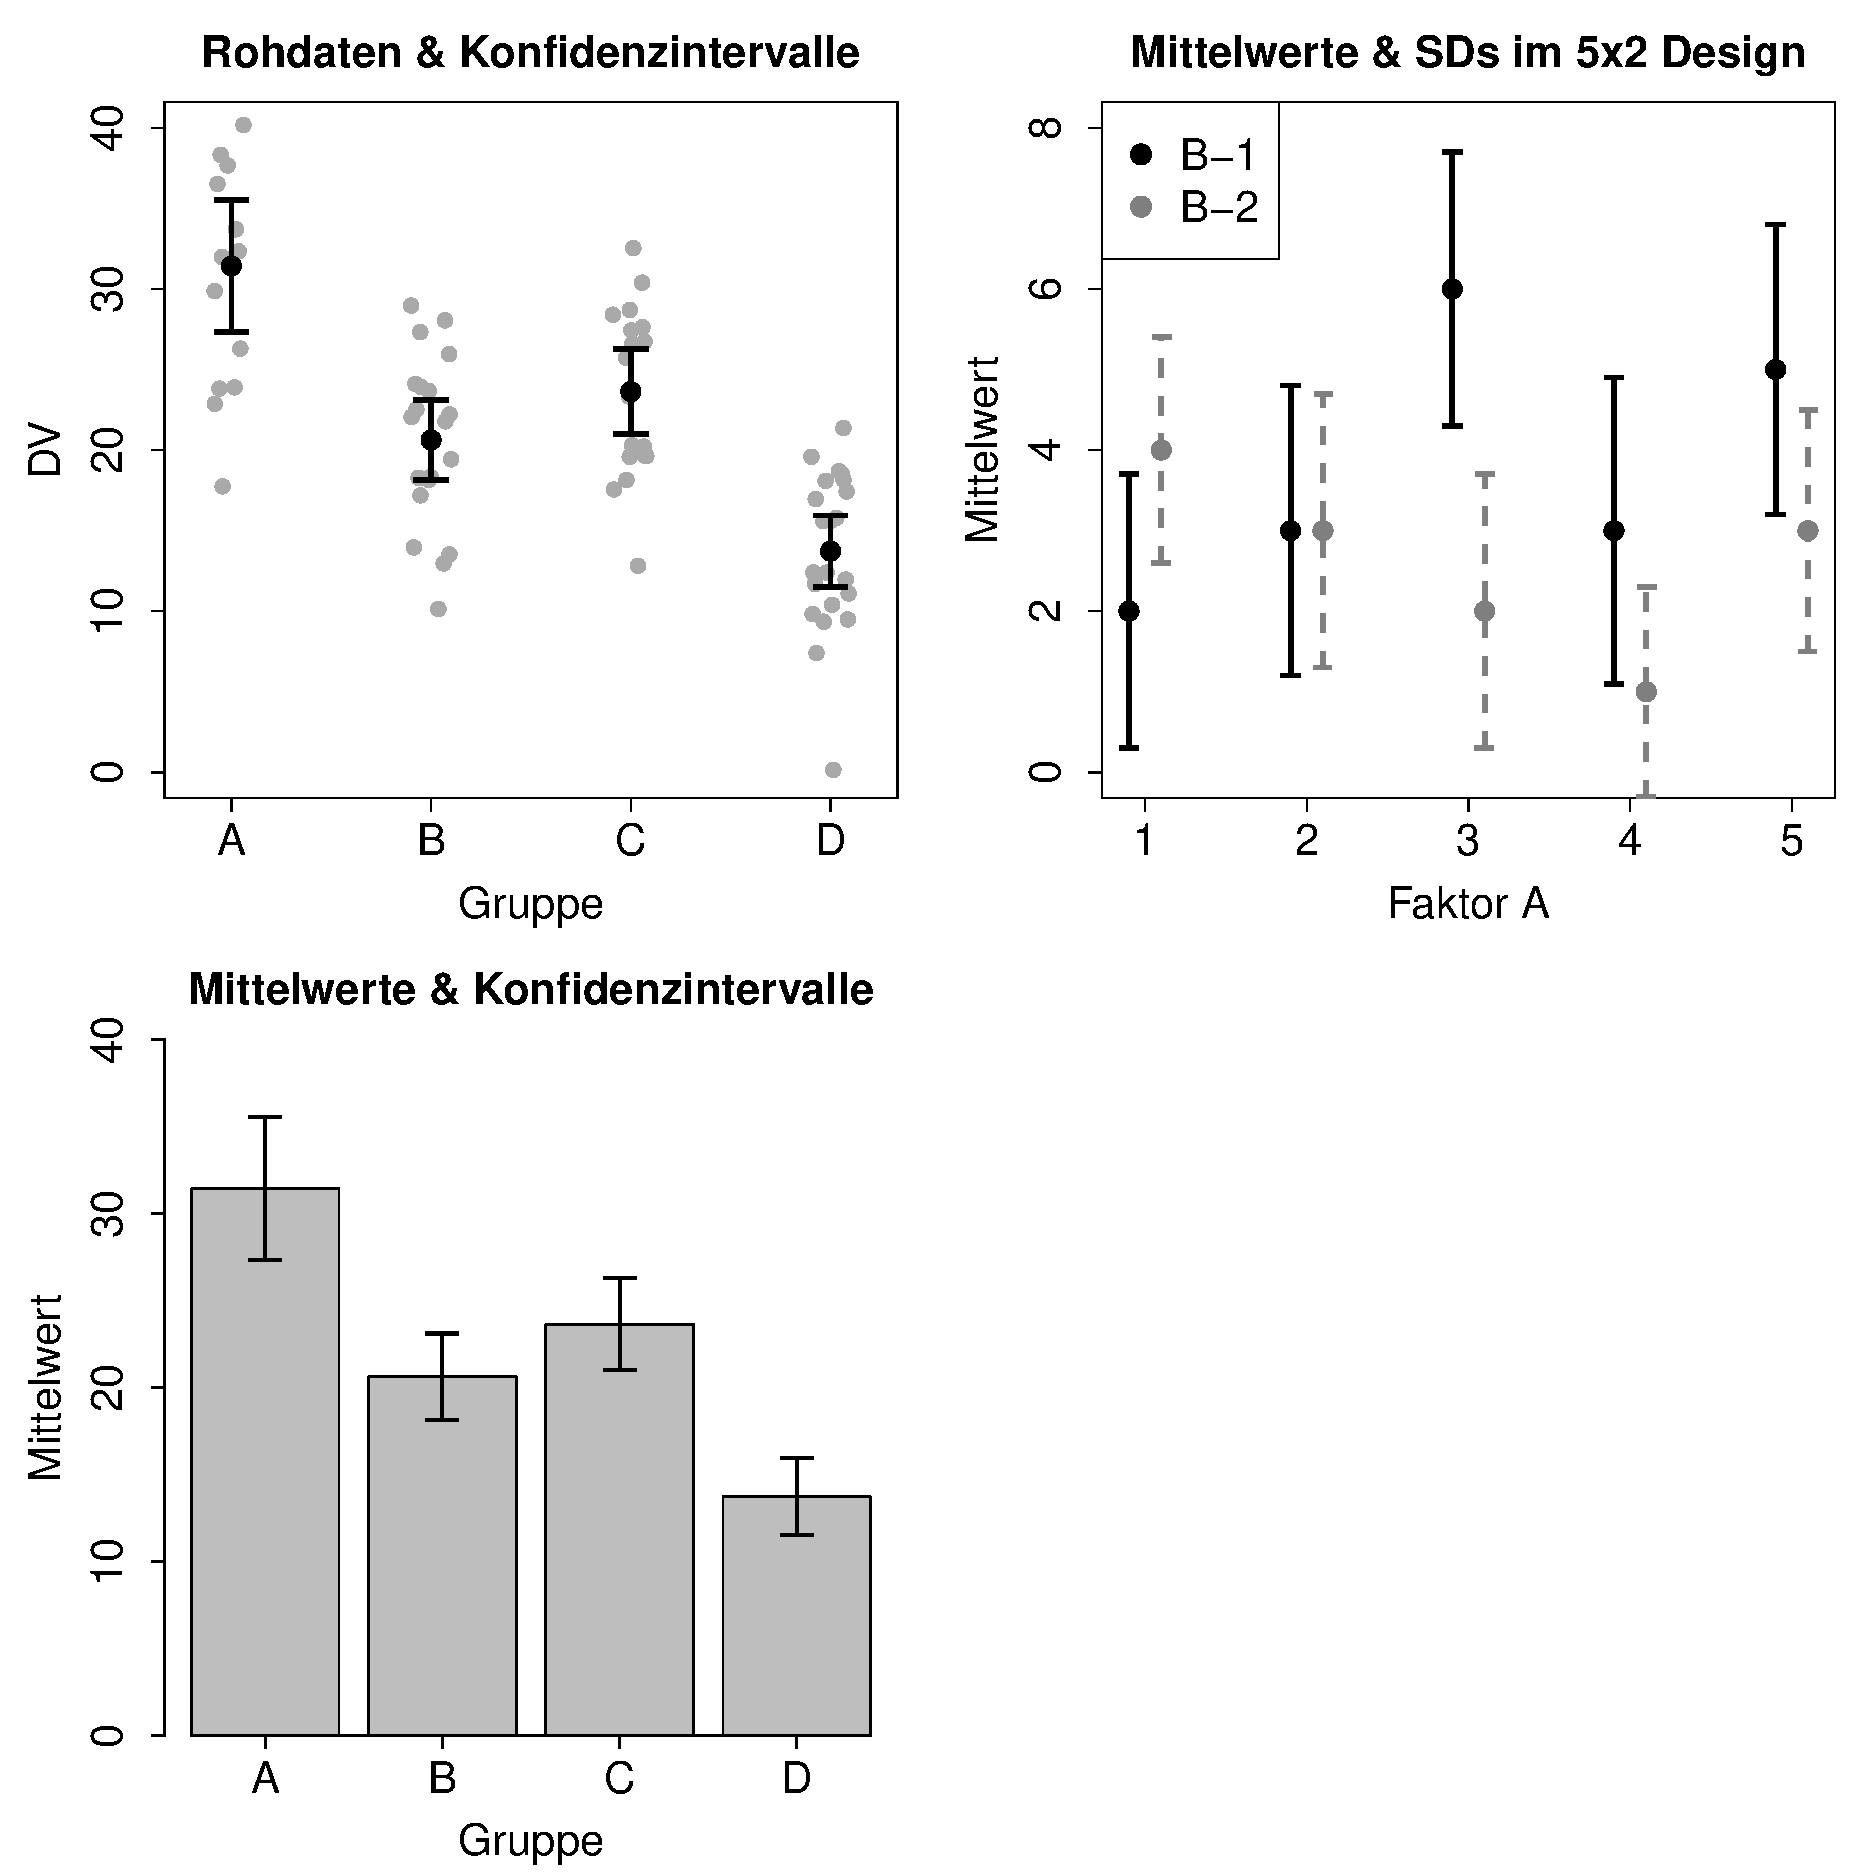
\includegraphics[width=12.5cm]{errorbars}
\vspace*{-0.5em}
\caption{Fehlerbalken mit \lstinline!ErrBars()! oder als Pfeile einfügen}
\label{fig:errorbars}
\end{figure}

Um selbst konstruierte Fehlerbalken in ein Diagramm einzufügen, können mit \lstinline!arrows()! erstellte Pfeile {\quotedblbase}zweckentfremdet{\textquotedblleft} werden (Abschn.\ \ref{sec:lines}). Pfeilen lässt sich das Aussehen von Fehlerbalken geben, indem an beiden Enden Pfeilspitzen gezeichnet werden (\lstinline!code=3!), für deren Winkel $90^{\circ}$ zu wählen (\lstinline!angle=90!) und deren Länge zu verkürzen ist (\lstinline!length=0.1!, Abb.\ \ref{fig:errorbars}). Die benötigten $x$-Koordinaten der Fehlerbalken sind im von \lstinline!barplot()! zurückgegebenen Vektor enthalten. Bei einem gruppierten Säulendiagramm handelt es sich stattdessen um eine Matrix. Die Höhe der Säulen liefert den vertikalen Mittelpunkt der Fehlerbalken und ergibt sich direkt aus den Daten, ebenso die $y$-Koordinaten der Endpunkte der Fehlerbalken als Grenzen des Konfidenzintervalls für den geschätzten statistischen Kennwert.
\begin{lstlisting}
# Säulendiagramm
> barsX <- barplot(height=Mj, xaxt="n", xlab="Gruppe", ylim=c(0, 40),
+          ylab="Mittelwert", main="Mittelwerte & Konfidenzintervalle")

> axis(side=1, at=barsX, labels=LETTERS[1:P])    # Gruppenbezeichnungen
> ciLo <- Mj - ciWidths                    # Fehlerbalken untere Grenze
> ciHi <- Mj + ciWidths                    # Fehlerbalken obere Grenze

# Fehlerbalken mit arrows()
> arrows(x0=barsX, y0=ciLo, x1=barsX, y1=ciHi,
+         code=3, angle=90, length=0.1, col="blue")
\end{lstlisting}

%%%%%%%%%%%%%%%%%%%%%%%%%%%%%%%%%%%%%%%%%%%%%%%%%%%%%%%%%%%%%%%%%%
%%%%%%%%%%%%%%%%%%%%%%%%%%%%%%%%%%%%%%%%%%%%%%%%%%%%%%%%%%%%%%%%%%
\subsection{Rastergrafiken}
\label{sec:rasterIm}
%%%%%%%%%%%%%%%%%%%%%%%%%%%%%%%%%%%%%%%%%%%%%%%%%%%%%%%%%%%%%%%%%%
%%%%%%%%%%%%%%%%%%%%%%%%%%%%%%%%%%%%%%%%%%%%%%%%%%%%%%%%%%%%%%%%%%

\index{Grafik!Rastergrafik}
Rastergrafiken definieren ein Bild als Ansammlung diskreter Bildpunkte (\emph{pixel} -- \emph{picture elements}), während Vektorgrafiken dies durch eine strukturelle Beschreibung der im Bild dargestellten Objekte tun. Für jeden Bildpunkt speichern Rastergrafiken den Farbwert, den das Bild an diesem Punkt besitzen soll. Rastergrafiken werden auch als Bitmap- bzw.\ Pixel-Grafiken bezeichnet. Sie lassen sich in zwei Schritten erzeugen und darstellen: Zunächst ist eine Matrix mit Farbwerten zu füllen, wobei jedes ihrer Elemente einen Bildpunkt festlegt. \lstinline!rasterImage()!\index[func]{rasterImage()@\lstinline{rasterImage()}} fügt das so definierte Bild dann einem bestehenden Diagramm hinzu (Abb.\ \ref{fig:rasterIm}).\footnote{Als Grafikdatei vorhandene Bitmap-Bilder können mit Funktionen aus den Paketen \lstinline!imager!\index[pack]{imager@\lstinline{imager}|textbf} \cite{Barthelme2019} oder \lstinline!EBImage!\index[pack]{EBImage@\lstinline{EBImage}|textbf} \cite{Pau2010} eingelesen werden.}
\begin{lstlisting}
rasterImage(image=<<Farb-Matrix>>,
             xleft=<<x-Koordinate>>,  ybottom=<<y-Koordinate>>,
            xright=<<x-Koordinate>>,     ytop=<<y-Koordinate>>,
            angle=<<Drehwinkel>>, interpolate=TRUE)
\end{lstlisting}

An \lstinline!image! ist eine Matrix mit Farbwerten zu übergeben (Abschn.\ \ref{sec:colors}). Anstatt die Farbwerte direkt in eine Matrix zu schreiben, lässt sich auch eine Matrix bzw.\ ein array mit Zahlen im Bereich von $0$--$1$ mit Hilfe von\index[func]{as.raster()@\lstinline{as.raster()}} \lstinline!as.raster()! in eine solche Farbwert-Matrix umwandeln. Wird dabei eine Matrix übergeben, symbolisiert jede Zahl den Grauwert eines Bildpunkts. Für farbige Bilder ist ein array mit drei Ebenen zu verwenden: Die Matrix der ersten Ebene definiert den Rot-Anteil, die der zweiten Ebene den Grün- und die der dritten Ebene den Blau-Anteil der Farbe jedes Bildpunkts.

Mit den Argumenten \lstinline!xleft! und \lstinline!ybottom! werden die $(x, y)$-Koordinaten der Position im Diagramm definiert, an der die linke untere Bildecke liegen soll, mit \lstinline!xright! und \lstinline!ytop! entsprechend die Koordinaten für die rechte obere Bildecke. \lstinline!angle! erlaubt es mit einer Winkelangabe in Grad, die Rastergrafik gegen den Uhrzeigersinn um die linke untere Bildecke zu drehen. Der über die Koordinaten der Bildecken ausgewählte Bereich des Diagramms kann in der Darstellung letztlich mehr oder weniger Bildpunkte abdecken, als in \lstinline!image! definiert sind. Das Bild muss deshalb auf den Abbildungsbereich gestreckt oder gestaucht werden. In der Voreinstellung \lstinline!interpolate=TRUE! wird beim Strecken linear zwischen der Farbe vormals angrenzender Bildpunkte interpoliert, was in etwas weniger abrupten Farbabstufungen resultiert.

\begin{figure}[ht]
\centering
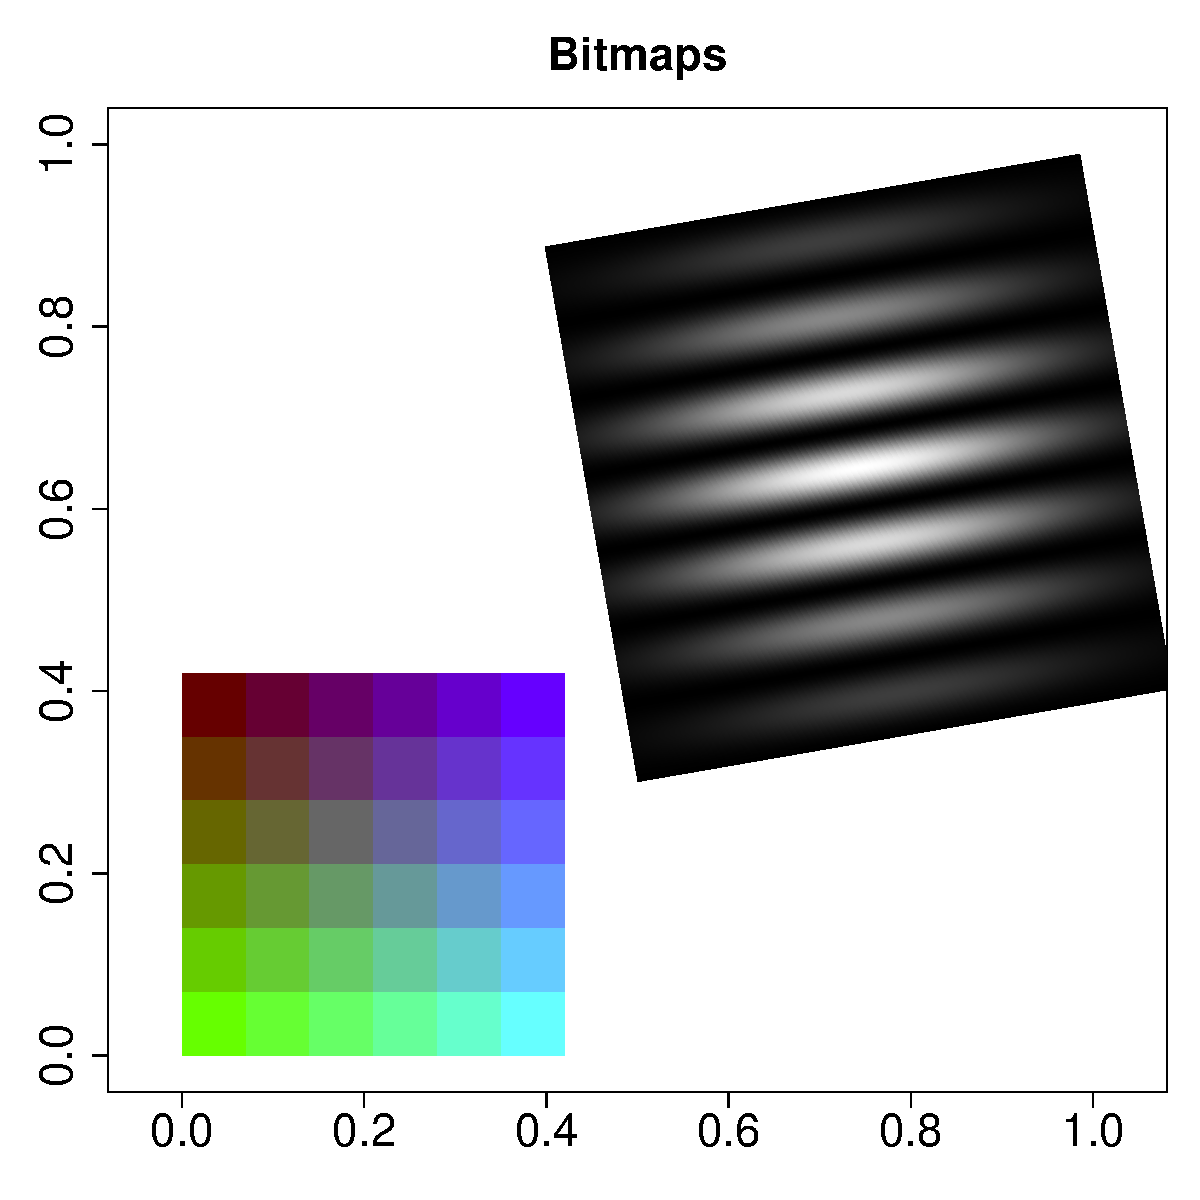
\includegraphics[width=8cm]{rasterIm}
\vspace*{-1em}
\caption{Rastergrafiken in einem Diagramm anzeigen}
\label{fig:rasterIm}
\end{figure}

Im Beispiel soll ein Bild aus farbigen Rechtecken und zusätzlich eine Gabor-Funktion dargestellt werden, also eine orientierte zweidimensionale Cosinus-Funktion, deren Amplitude einer zweidimensionalen Normalverteilung folgt.
\begin{lstlisting}
> pxSq  <- 6                         # Anzahl Bildpunkte pro Achse
> colsR <- rep(0.4, pxSq^2)          # Rot-Anteil: hier konstant
> colsG <- rep(seq(0, 1, length.out=pxSq), times=pxSq)          # Grün
> colsB <- rep(seq(0, 1, length.out=pxSq), each=pxSq)           # Blau

# array mit drei Ebenen: Rot, Grün, Blau
> arrSq <- array(c(colsR, colsG, colsB), c(pxSq, pxSq, 3))
> sqIm   - as.raster(arrSq)          # Zahlen -> Farbwerte

# Gabor-Funktion
> pxGab <- 500                       # Anzahl Bildpunkte pro Achse
> alpha <- 0.5                       # Faktor für Winkel 2D-Cosinus
> beta  <- min(c(1-alpha, 1+alpha))  # für komplementären Winkel
> freq  <- 3.5                       # Frequenz 2D-Cosinus

# x- und y-Wertebereich für 2D-Cosinus und 2D-Normalverteilung
> vals <- rep(seq(-2*pi, 2*pi, length.out=pxGab), pxGab)

# Matrizen mit den x- bzw. y-Koordinaten aller Bildpunkte
> x   <- matrix(vals, nrow=pxGab, byrow=TRUE)
> y   <- matrix(vals, nrow=pxGab, byrow=FALSE)
> phi <- alpha*x + beta*y            # konvexe Mischung der Koordinaten

# 2D-Cosinus skaliert auf Werte im Bereich [0, 1]
> cosMat <- 0.5*cos(freq*phi) + 0.5

# Werte unkorrelierter 2D-Normalverteilung
> library(mvtnorm)                   # für dmvnorm()
> mu       <- c(0, 0)                # Zentroid
> sigma    <- diag(2)*10             # Kovarianzmatrix
> gaussVal <- dmvnorm(cbind(c(x), c(y)), mu, sigma)

# als Matrix skaliert auf Werte im Bereich [0, 1]
> gaussMat <- matrix(gaussVal, nrow=pxGab) / max(gaussVal)

# Gabor = Produkt von 2D-Cos und 2D-NV, Zahlen -> Farbwerte
> gabIm <- as.raster(cosMat*gaussMat)

# öffne leeres Diagramm
> plot(c(0, 1), c(0, 1), type="n",
+      main="Bitmaps", xlab="", ylab="", asp=1)

# füge Matrizen mit Farbwerten als Rastergrafiken ein
> rasterImage(sqIm,    0, 0,   0.3, 0.3, angle=0,  interpolate=FALSE)
> rasterImage(gabIm, 0.5, 0.3, 1.1, 0.9, angle=10, interpolate=TRUE)
\end{lstlisting}

\index{Grafik!Bildbearbeitung}
\index{Signalverarbeitung}
R verfügt auch über die grundlegenden Funktionen zur digitalen Signalverarbeitung, die sich insbesondere zur Bildanalyse und -manipulation eignen: Mit \index[func]{fft()@\lstinline{fft()}} \lstinline!fft()! ist die schnelle\index{Fourier-Transformation} Fourier-Transformation und ihre Rücktransformation möglich, der\index{Faltung} Faltungsoperator ist in\index[func]{convolve()@\lstinline{convolve()}} \lstinline!convolve()! implementiert. Für weitere Funktionen vgl.\ die Pakete \lstinline!imager!\index[pack]{imager@\lstinline{imager}} und \lstinline!EBImage!\index[pack]{EBImage@\lstinline{EBImage}}.

%%%%%%%%%%%%%%%%%%%%%%%%%%%%%%%%%%%%%%%%%%%%%%%%%%%%%%%%%%%%%%%%%%
%%%%%%%%%%%%%%%%%%%%%%%%%%%%%%%%%%%%%%%%%%%%%%%%%%%%%%%%%%%%%%%%%%
\section{Verteilungsdiagramme}
\label{sec:distDiag}
%%%%%%%%%%%%%%%%%%%%%%%%%%%%%%%%%%%%%%%%%%%%%%%%%%%%%%%%%%%%%%%%%%
%%%%%%%%%%%%%%%%%%%%%%%%%%%%%%%%%%%%%%%%%%%%%%%%%%%%%%%%%%%%%%%%%%

\index{Daten!Ausreißer}
Verteilungsdiagramme dienen dazu, sich einen Überblick über die Lage und Verteilungsform der in einer Stichprobe erhobenen Daten zu verschaffen. Sie eignen sich damit auch zur Überprüfung der Daten auf Ausreißer oder unplausible Werte, die etwa aus Eingabefehlern herrühren können (Abschn.\ \ref{sec:tidyData}). Dies kann entweder anhand summarischer Kennwerte oder aber durch Darstellung von Einzelwerten, ggf.\ in vergröberter Form, geschehen.

%%%%%%%%%%%%%%%%%%%%%%%%%%%%%%%%%%%%%%%%%%%%%%%%%%%%%%%%%%%%%%%%%%
%%%%%%%%%%%%%%%%%%%%%%%%%%%%%%%%%%%%%%%%%%%%%%%%%%%%%%%%%%%%%%%%%%
\subsection{Histogramm und Schätzung der Dichtefunktion}
\label{sec:hist}
%%%%%%%%%%%%%%%%%%%%%%%%%%%%%%%%%%%%%%%%%%%%%%%%%%%%%%%%%%%%%%%%%%
%%%%%%%%%%%%%%%%%%%%%%%%%%%%%%%%%%%%%%%%%%%%%%%%%%%%%%%%%%%%%%%%%%

\index{Grafik!Histogramm}
\index{Histogramm|see{Grafik}}
Für Stichproben stetiger Variablen, die eine Vielzahl unterschiedlicher Werte enthalten, kann ein Histogramm als Sonderform eines Säulendiagramms für die Darstellung der empirischen Häufigkeitsverteilung verwendet werden. Histogramme stellen nicht die Häufigkeit einzelner Werte, sondern die von Wertebereichen (disjunkten Intervallen) anhand von Säulen dar, zwischen denen kein Zwischenraum ist\index[func]{hist()@\lstinline{hist()}} (Abb.\ \ref{fig:hist}).\footnote{\lstinline!PlotFdist()!\index[func]{PlotFdist()@\lstinline{PlotFdist()}} aus dem Paket \lstinline!DescTools!\index[pack]{DescTools@\lstinline{DescTools}} stellt das Histogramm gemeinsam mit der kumulierten empirischen Häufigkeitsverteilung sowie einem boxplot in einem Diagramm dar. Für den Vergleich der Verteilungen einer Variable in zwei Bedingungen zeigt\index[func]{histbackback()@\lstinline{histbackback()}} \lstinline!histbackback()! aus dem\index[pack]{Hmisc@\lstinline{Hmisc}} \lstinline!Hmisc! Paket die zugehörigen Histogramme Rücken-an-Rücken angeordnet simultan in einem Diagramm.}
\begin{lstlisting}
hist(x=<<Vektor>>, breaks=<<Grenzen>>, freq=NULL)
\end{lstlisting}

Die Daten sind in Form eines Vektors \lstinline!x! zu übergeben. Die Intervallgrenzen werden über das Argument \lstinline!breaks! festgelegt, wobei mit einer einzelnen Zahl deren Anzahl und mit einem Vektor deren genaue Lage vorgegeben werden kann. In der Voreinstellung wird beides nach einem in der Hilfe beschriebenen Algorithmus entsprechend den Daten in \lstinline!x! gewählt.\footnote{Wird die Anzahl der Klassengrenzen genannt, behandelt R diesen Wert nur als Vorschlag, nicht als zwingend. Der in der Voreinstellung verwendete Algorithmus erzeugt häufig nur wenige Intervalle. Durch \lstinline!breaks="FD"! wird ein anderer Algorithmus verwendet, der meist zu einer etwas größeren Anzahl führt.} Bei gleichabständigen Klassengrenzen werden in der Voreinstellung \lstinline!freq=NULL! absolute Häufigkeiten angezeigt. Mit \lstinline!freq=FALSE! sind es stattdessen die Dichten, also die relativen Häufigkeiten geteilt durch die Klassenbreite. \lstinline!TRUE! erzwingt absolute Häufigkeiten auch bei ungleichen Klassenbreiten. Der auf der Konsole nicht sichtbare Rückgabewert von \lstinline!hist()! enthält in Form einer Liste u.\,a.\ Angaben zur Lage und Besetzung der verwendeten Intervalle.
\begin{lstlisting}
> height <- rnorm(100, mean=175, sd=7)       # Körpergröße 100 Personen
> hist(height, xlab="height [cm]", ylab="N")
\end{lstlisting}

Für die individuelle Wahl der Klassengrenzen empfiehlt es sich, zunächst die Spannweite der Daten auszuwerten. Intervallgrenzen in regelmäßigen Abständen können dann z.\,B.\ mit \lstinline!seq()! generiert werden. Werte, die genau auf einer Grenze liegen, werden immer der unteren Klasse zugeordnet, die Klassen sind also nach unten offene und nach oben geschlossene Intervalle.
\begin{lstlisting}
# darzustellender Wertebereich
> fromTo <- round(range(height), -1) + c(-10, 10)
> limits <- seq(from=fromTo[1], to=fromTo[2], by=5)  # Intervallgrenzen
> hist(height, freq=FALSE, xlim=fromTo, xlab="height [cm]",
+      ylab="relative Häufigkeit", breaks=limits,
+      main="Histogramm & Normalverteilung")
\end{lstlisting}

Als weitere Information lässt sich im Anschluss an den Aufruf von \lstinline!hist()! mit\index[func]{rug()@\lstinline{rug()}} \lstinline!rug()! auch die Lage der Einzelwerte mit darstellen. Dies geschieht in Form senkrechter Striche entlang der Abszisse, wobei jeder Strich für einen Wert steht. Um Bindungen in Form separater Striche in ihre Einzelwerte aufzulösen, sollte die Funktion mit\index[func]{jitter()@\lstinline{jitter()}} \lstinline!jitter()! gekoppelt werden. Diese Funktion verändert die Werte um einen kleinen zufälligen Betrag, wodurch sich die Lage der Striche horizontal leicht verschiebt. Dies führt zu dickeren Strichen als Repräsentation der Bindungen.
\begin{lstlisting}
> rug(jitter(height))
\end{lstlisting}

Soll über das Histogramm zum Vergleich eine theoretisch vermutete Dichtefunktion gelegt werden, kann diese etwa mit \lstinline!curve(..., add=TRUE)! hinzugefügt werden. Für eine passende Skalierung muss das Histogramm mit \lstinline!freq=FALSE! die Dichte darstellen.
\begin{lstlisting}
# füge Dichtefunktion einer Normalverteilung hinzu
> curve(dnorm(x, mean(height), sd(height)), lwd=2, col="blue", add=TRUE)
\end{lstlisting}

Die Wahl der Intervallgrenzen hat einen starken Einfluss auf die Form von Histogrammen. Aufgrund dieser Abhängigkeit von einem willkürlich festzulegenden Parameter eignen sich Histogramme nicht immer gut, um sich einen Eindruck von der empirischen Verteilung einer Variable zu verschaffen.

\index{Verteilung!Dichtefunktion schätzen}
Als Alternative lässt sich mit \index[func]{density()@\lstinline{density()}} \lstinline!density(<<Vektor>>)! auf Basis einer im Vektor gespeicherten Stichprobe von Werten die Dichtefunktion der zugehörigen Variable schätzen und grafisch darstellen (Abschn.\ \ref{sec:density}).\footnote{Zweidimensionale Dichten werden von \index[func]{smoothScatter()@\lstinline{smoothScatter()}} \lstinline!smoothScatter()! geschätzt und dargestellt.} Über \lstinline!plot(density(<<Vektor>>))! wird die Schätzung der Dichtefunktion grafisch in einem separaten Diagramm veranschaulicht, während \lstinline!lines(density(<<Vektor>>))! die geschätzte Dichtefunktion einem bereits geöffneten Diagramm hinzufügt. Bei einem Histogramm ist dabei darauf zu achten, für die Darstellung Dichte das Argument \lstinline!freq=FALSE! zu setzen.
\begin{lstlisting}
> hist(height, freq=FALSE, xlim=fromTo, xlab="height [cm]",
+      main="Histogramm & Dichte-Schätzung")

> lines(density(height, bw="SJ"), lwd=2, col="blue")
> rug(jitter(height))
\end{lstlisting}

\begin{figure}[ht]
\centering
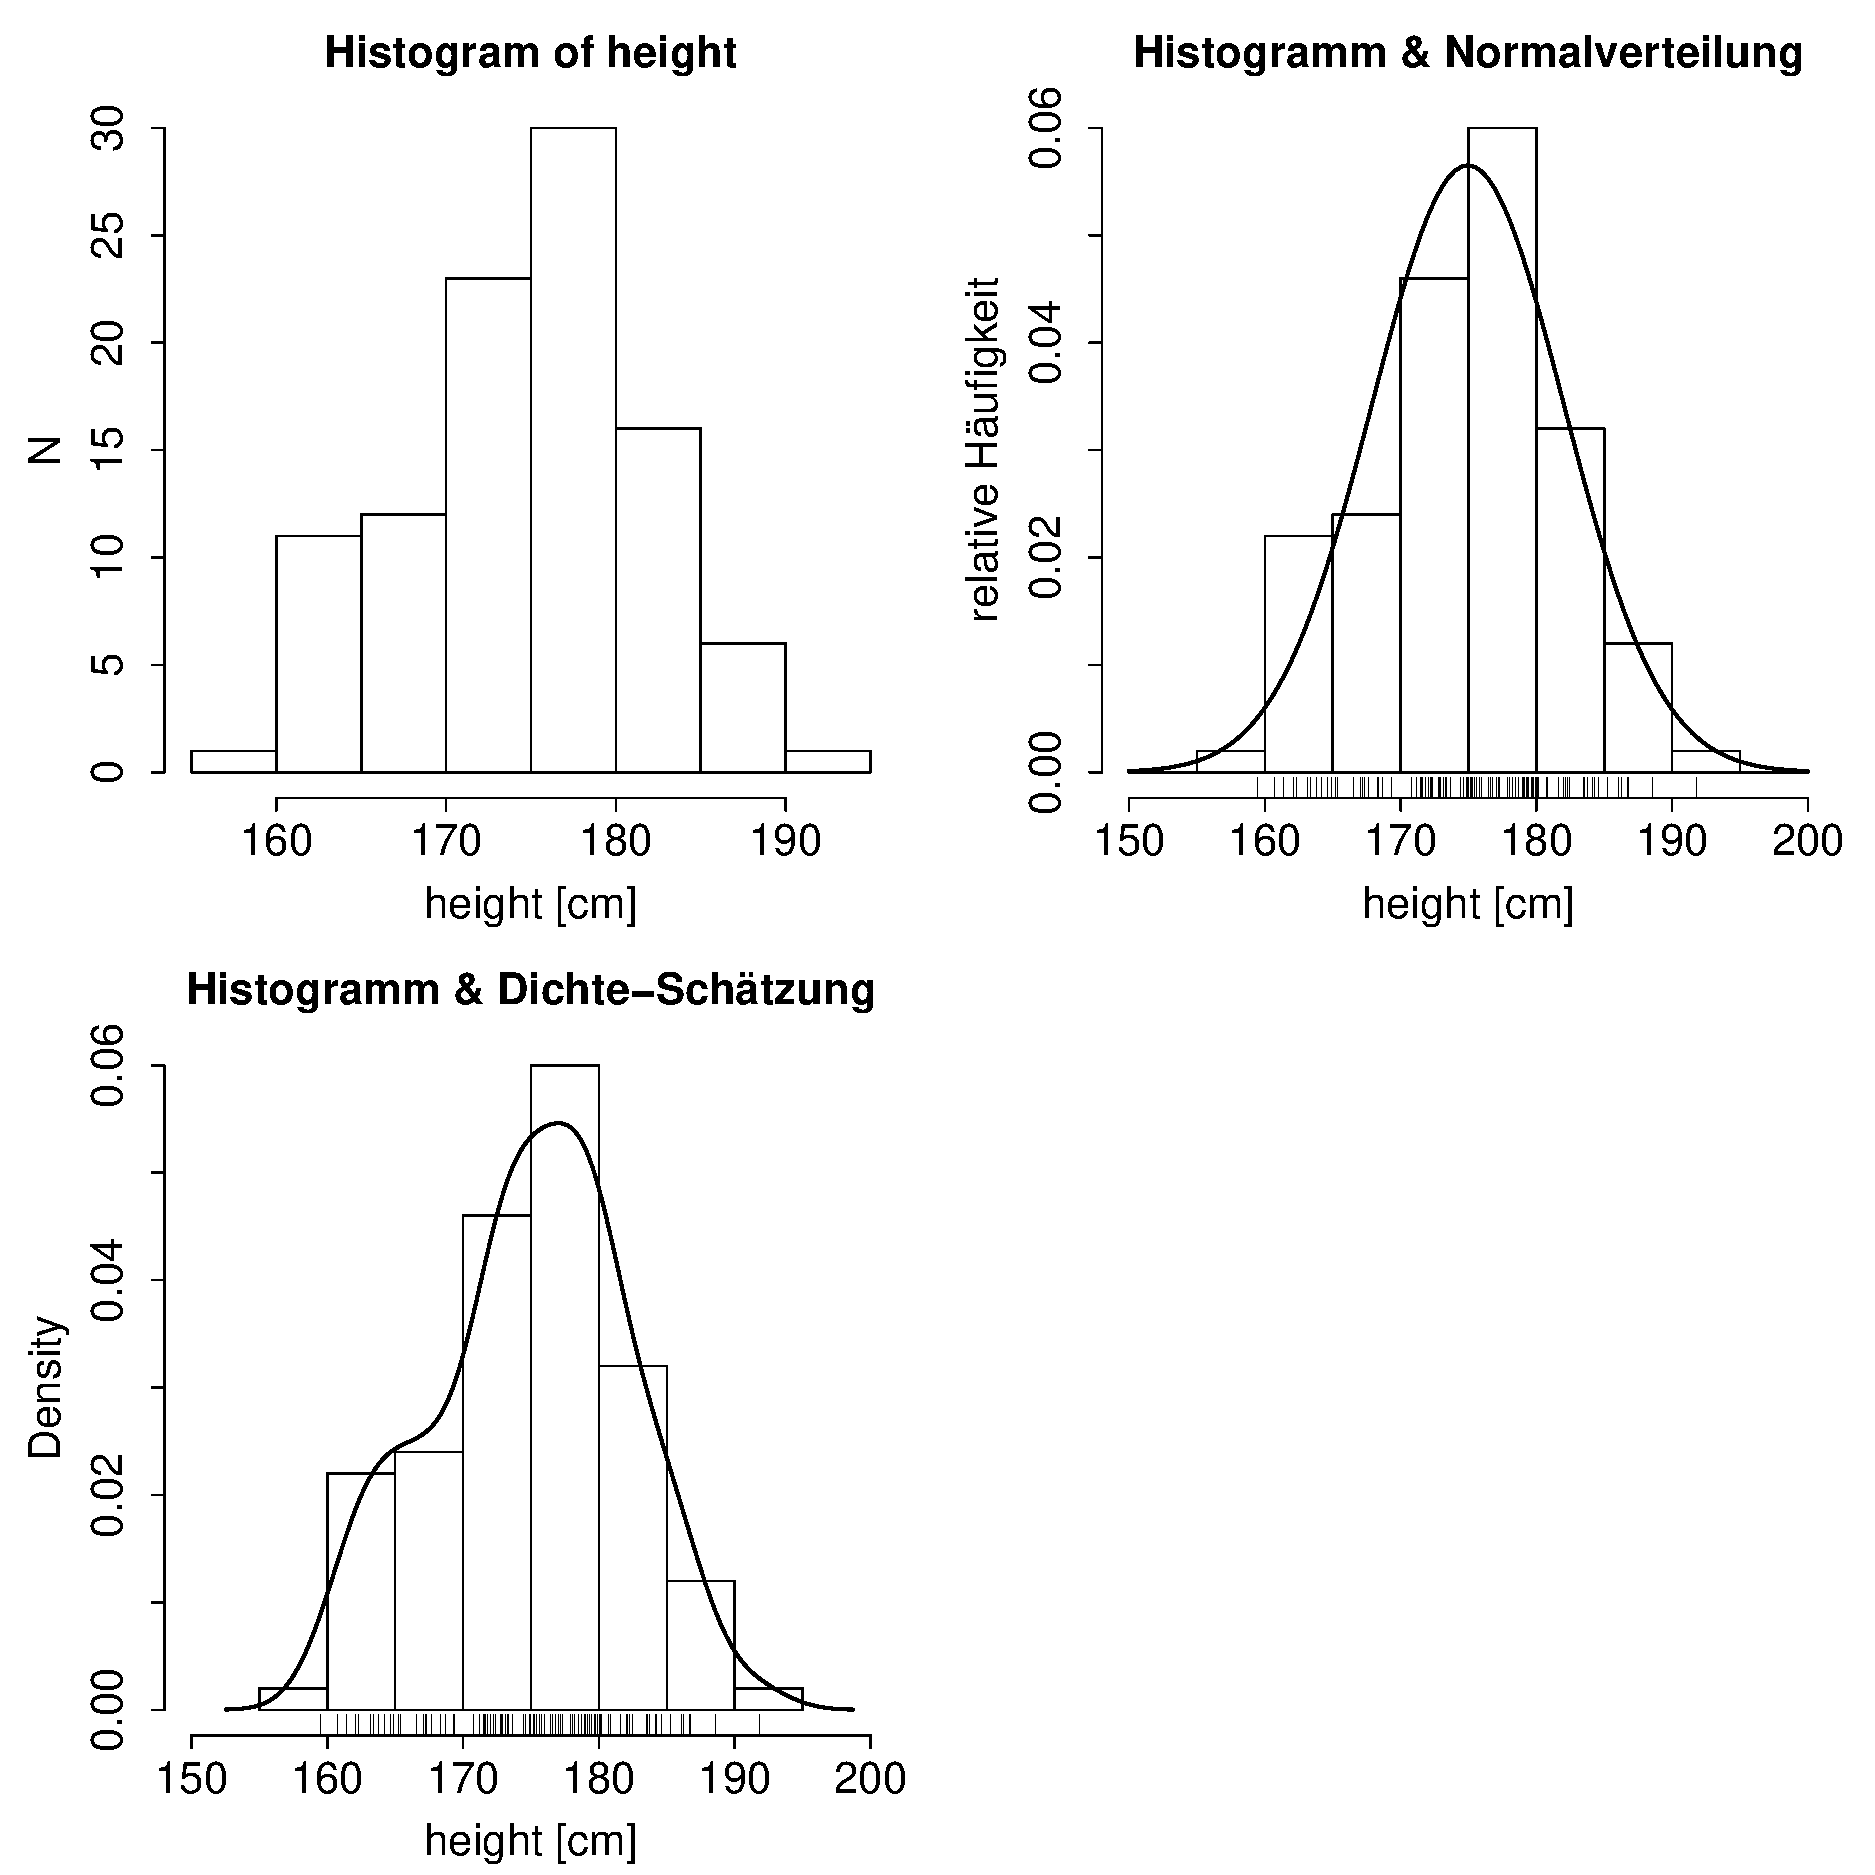
\includegraphics[width=12.5cm]{hist}
\vspace*{-1em}
\caption{Histogramm, zusätzlich mit Einzelwerten und Normalverteilung bzw.\ mit Schätzung der Dichtefunktion}
\label{fig:hist}
\end{figure}

%%%%%%%%%%%%%%%%%%%%%%%%%%%%%%%%%%%%%%%%%%%%%%%%%%%%%%%%%%%%%%%%%%
%%%%%%%%%%%%%%%%%%%%%%%%%%%%%%%%%%%%%%%%%%%%%%%%%%%%%%%%%%%%%%%%%%
\subsection{Stamm-Blatt-Diagramm}
%%%%%%%%%%%%%%%%%%%%%%%%%%%%%%%%%%%%%%%%%%%%%%%%%%%%%%%%%%%%%%%%%%
%%%%%%%%%%%%%%%%%%%%%%%%%%%%%%%%%%%%%%%%%%%%%%%%%%%%%%%%%%%%%%%%%%

\index{Grafik!Stamm-Blatt-Diagramm}
Das Stamm-Blatt-Diagramm mischt die Darstellung von Häufigkeiten einzelner Werte mit einem Histogramm. Seine Ausgabe erfolgt nicht in einem device, sondern in Textform auf der Konsole. Der Wertebereich wird dafür zunächst wie bei einem Histogramm in disjunkte Intervalle eingeteilt, die dieselbe Breite besitzen. Diese Intervalle bilden den \emph{Stamm} und werden durch die Ziffernfolge repräsentiert, mit der alle Werte im Intervall beginnen. Geht das erste Intervall etwa von $120$ bis (ausschließlich) $130$, ist der Wert des Stamms $12$. Die \emph{Blätter} werden dann jeweils durch jene Werte gebildet, die in dasselbe Intervall fallen und durch die auf den Stamm folgende Ziffer repräsentiert. Dabei werden die Werte zunächst auf die Stelle gerundet, die auf den Stamm folgt. Insgesamt repräsentiert also jedes Blatt einen Wert der Stichprobe.

\index[func]{stem()@\lstinline{stem()}}
\begin{lstlisting}
stem(x=<<Vektor>>, scale=1, width=80, atom=1e-08)
\end{lstlisting}

Unter \lstinline!x! wird der Datenvektor eingetragen. Mit \lstinline!scale! kann die Anzahl der Intervalle in Form eines Skalierungsfaktors verändert werden. \lstinline!width! legt mit Werten $> 10$ fest, wie viele Blätter maximal gezeigt werden, wobei diese Anzahl \lstinline!width-10! beträgt. Bei Werten für \lstinline!width! $\leq 10$ werden keine Blätter angezeigt -- es wird nur vermerkt, ob mehr als \lstinline!width! Werte im Intervall liegen und ggf.\ wie viele dies sind. Unter \lstinline!atom! wird die Genauigkeit der Unterscheidung zwischen den einzelnen Werten definiert. Per Voreinstellung wird bis zur achten Nachkommastelle unterschieden.
\begin{lstlisting}
> stem(rnorm(100, mean=175, sd=7))
The decimal point is 1 digit(s) to the right of the |

15 | 8
16 | 12344
16 | 5556678888999999
17 | 001111122222222223334444
17 | 555555555666666777777788889999999
18 | 00001223333444
18 | 5666899
\end{lstlisting}

Aus der Konstruktion des Diagramms folgt, dass die Kombination des Stammes mit einem zugehörigen Blatt einen Wert von \lstinline!x! repräsentiert, weswegen sich alle Werte der Stichprobe aus dem Diagramm (bis auf die Rundung) rekonstruieren lassen. Ist der Stamm \lstinline!15! und ein Blatt \lstinline!8!, wird etwa der Wert $158$ dargestellt -- in Abhängigkeit von der Lage der Dezimalstelle, über die in der Diagrammüberschrift informiert wird.

%%%%%%%%%%%%%%%%%%%%%%%%%%%%%%%%%%%%%%%%%%%%%%%%%%%%%%%%%%%%%%%%%%
%%%%%%%%%%%%%%%%%%%%%%%%%%%%%%%%%%%%%%%%%%%%%%%%%%%%%%%%%%%%%%%%%%
\subsection{Boxplot}
\label{sec:boxplot}
%%%%%%%%%%%%%%%%%%%%%%%%%%%%%%%%%%%%%%%%%%%%%%%%%%%%%%%%%%%%%%%%%%
%%%%%%%%%%%%%%%%%%%%%%%%%%%%%%%%%%%%%%%%%%%%%%%%%%%%%%%%%%%%%%%%%%

\index{Grafik!boxplot}
\index{Boxplot|see{Grafik}}
Ein boxplot (\emph{box-whisker-plot}) stellt die Lage und Verteilung empirischer Daten durch die gleichzeitige Visualisierung verschiedener Kennwerte dar. Der Median wird dabei durch eine schwarze horizontale Linie innerhalb einer Box gekennzeichnet, deren untere Grenze sich auf Höhe des ersten und deren obere Grenze sich auf Höhe des dritten Quartils befindet.\footnote{Liegen geradzahlig viele Werte vor, wird das Rechteck nach oben und unten nicht exakt durch die Quartile begrenzt, vgl.\ \lstinline!?boxplot.stats!.} Innerhalb des so gebildeten Rechtecks liegen damit die mittleren $50\%$ der Werte, seine Höhe ist gleich dem Interquartilabstand. Jenseits der Box erstrecken sich nach oben und unten dünne Striche (\emph{whiskers}), deren Enden jeweils den extremsten Wert angeben, der noch keinen Ausreißer darstellt. Als Ausreißer werden dabei in der Voreinstellung solche Werte betrachtet, die um mehr als das Anderthalbfache des Interquartilabstands unter oder über der Box liegen. Solche Ausreißer werden schließlich durch Kreise gekennzeichnet.

Boxplots sind u.\,a.\ dazu geeignet, Symmetrie bzw.\ Schiefe unimodaler Verteilungen zu beurteilen. Zudem lassen sich Lage und Verteilung einer Variable für mehrere Gruppen getrennt vergleichen, indem die zugehörigen boxplots nebeneinander in ein Diagramm gezeichnet werden\index[func]{boxplot()@\lstinline{boxplot()}} (Abb.\ \ref{fig:boxplot}).
\begin{lstlisting}
boxplot(x=<<Vektor>>, range=<<Zahl>>, notch=FALSE, horizontal=FALSE)
\end{lstlisting}

Bei einem einzelnen boxplot wird unter \lstinline!x! der Datenvektor eingegeben. Stattdessen kann für \lstinline!x! auch eine Modellformel der Form \lstinline!<<Messwerte>> ~ <<Faktor>>! übergeben werden, wobei \lstinline!<<Faktor>>! dieselbe Länge wie der Vektor \lstinline!<<Messwerte>>! besitzt und für jeden von dessen Werten codiert, zu welcher Bedingung er gehört. Stammen die in der Modellformel verwendeten Variablen aus einem Datensatz, ist dieser unter \lstinline!data! zu nennen.  Hiermit werden getrennt für die von \lstinline!<<Faktor>>! definierten $n$ Gruppen boxplots nebeneinander in einem Diagramm dargestellt, wobei als $x$-Koordinaten die Zahlen $1, \ldots, n$ verwendet werden. Dasselbe Ergebnis lässt sich erzielen, indem an \lstinline!x! eine Matrix übergeben wird, deren Spalten die Gruppen definieren, für die jeweils ein boxplot darzustellen ist. Über das Argument \lstinline!range! wird die Definition eines Ausreißers als Vielfaches des Interquartilabstands kontrolliert. Das Argument \lstinline!notch! bestimmt, ob ein gekerbter boxplot gezeichnet werden soll. Für horizontal verlaufende Boxen ist \lstinline!horizontal=TRUE! zu setzen. Der auf der Konsole nicht sichtbare Rückgabewert enthält in Form einer Liste Angaben zu den dargestellten statistischen Kennwerten.
\begin{lstlisting}
> Nj <- 40                                        # Gruppengröße
> P  <- 3                                         # Anzahl Gruppen
> DV <- rnorm(P*Nj, mean=100, sd=15)              # Messwerte

# Faktor Gruppenzugehörigkeit
> IV <- gl(P, Nj, labels=c("Control", "Group A", "Group B"))
> Mj <- tapply(DV, IV, FUN=mean)                  # Gruppenmittel
> boxplot(DV ~ IV, ylab="Score", col=c("red", "blue", "green"),
+         main="Boxplots und Scores in 3 Gruppen")

> points(1:P, Mj, pch=16, cex=2)                  # zeige Gruppenmittel
\end{lstlisting}

Da boxplots wichtige Eigenschaften der Verteilung wie etwa Multimodalität nicht repräsentieren können, ist es oft sinnvoll, zusätzlich die Rohdaten darzustellen. \lstinline!beeswarm()!\index[func]{beeswarm()@\lstinline{beeswarm()}} aus dem Paket \lstinline!beeswarm!\index[pack]{beeswarm@\lstinline{beeswarm}} \cite{Eklund2016} zeigt alle einzelnen Datenpunkte, wobei die horizontale Position so versetzt gewählt wird, dass die Verteilungsform gut ersichtlich ist (Abb.\ \ref{fig:boxplot}). Der Aufruf erfolgt analog zu \lstinline!boxplot()!, wobei die Rohdaten mit der Option \lstinline!add=TRUE! einem schon bestehenden Diagramm hinzugefügt werden.

Damit Ausreißer nicht doppelt dargestellt werden, sollte man sie im Aufruf von \lstinline!boxplot()! mit der Option \lstinline!outline=FALSE! ausblenden. Der Darstellungsbereich der $y$-Achse muss dann gleichzeitig so gewählt werden, dass \lstinline!beeswarm()! anschließend die Ausreißer noch sichtbar darstellen kann.
\begin{lstlisting}
> library(beeswarm)                        # für beeswarm()
> DVrange <- round(range(DV), digits=-1)   # Darstellungsbereich y-Achse
> boxplot(DV ~ IV, ylab="Score", col=c("red", "blue", "green"),
+         main="Boxplots und Scores in 3 Gruppen",
+         outline=FALSE, ylim=DVrange)
 
> beeswarm(DV ~ IV, add=TRUE, pch=16, col="#00000077") # mit Transparenz
\end{lstlisting}

\begin{figure}[ht]
\centering
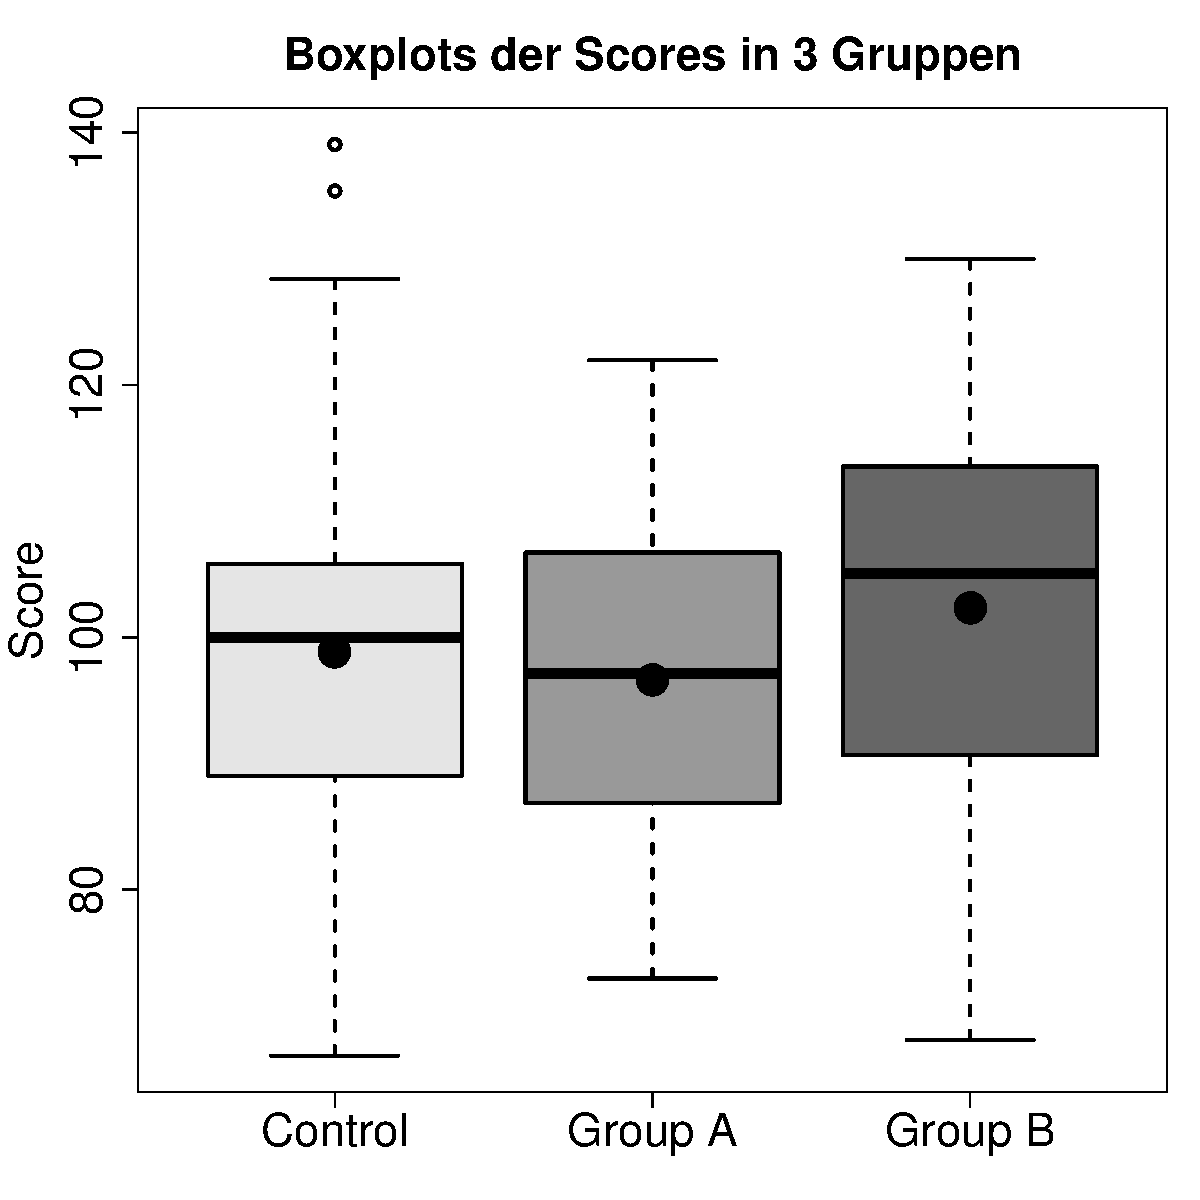
\includegraphics[width=12.5cm]{boxplot}
\vspace*{-1em}
\caption{Boxplots getrennt nach Gruppen mit Mittelwerten sowie zusätzlich den Einzelwerten}
\label{fig:boxplot}
\end{figure}

%%%%%%%%%%%%%%%%%%%%%%%%%%%%%%%%%%%%%%%%%%%%%%%%%%%%%%%%%%%%%%%%%%
%%%%%%%%%%%%%%%%%%%%%%%%%%%%%%%%%%%%%%%%%%%%%%%%%%%%%%%%%%%%%%%%%%
\subsection{Stripchart}
%%%%%%%%%%%%%%%%%%%%%%%%%%%%%%%%%%%%%%%%%%%%%%%%%%%%%%%%%%%%%%%%%%
%%%%%%%%%%%%%%%%%%%%%%%%%%%%%%%%%%%%%%%%%%%%%%%%%%%%%%%%%%%%%%%%%%

\index{Grafik!stripchart}
Ein mit\index[func]{stripchart()@\lstinline{stripchart()}} \lstinline!stripchart()! erstelltes eindimensionales Streudiagramm eignet sich zur Veranschaulichung der empirischen Verteilung quantitativer Variablen, wenn der Stichprobenumfang gering ist. Statt wie ein boxplot Daten summarisch anhand ihrer wichtigsten Verteilungsparameter zu illustrieren, stellt ein stripchart alle vorkommenden Werte selbst dar. Zu diesem Zweck wird jeder Einzelwert als Punkt auf einer horizontalen Achse repräsentiert, wobei der Wert die $x$-Koordinate des Punkts bestimmt (Abb.\ \ref{fig:stripchart}).
\begin{lstlisting}
stripchart(x=<<Vektor>>, method="overplot", vertical=FALSE, add=FALSE,
           at=<<Position>>)
\end{lstlisting}

Die im Diagramm einzutragenden Daten werden in Form eines Vektors für \lstinline!x! übergeben. In der Voreinstellung \lstinline!"overplot"! bewirkt das Argument \lstinline!method!, dass Bindungen durch dasselbe Symbol repräsentiert werden. Die so erstellte Grafik liefert damit keinen Aufschluss darüber, wie oft ein bestimmter Wert vorkommt. Um auch dies zu erreichen, gibt es zwei Methoden, die über das Argument \lstinline!method! kontrolliert werden. Auf \lstinline!"jitter"! gesetzt werden die Werte durch Symbole mit derselben $x$-Koordinate, aber einem zufälligen vertikalen Versatz dargestellt. Durch \lstinline!"stack"! werden die Symbole eines mehrfach vorkommenden Wertes vertikal gestapelt. Um im Diagramm die Rolle von $x$- und $y$-Achse zu vertauschen, kann das Argument \lstinline!vertical=TRUE! gesetzt werden.

Ein stripchart kann auch die Verteilung einer quantitativen Variable für mehrere Gruppen gleichzeitig veranschaulichen. Hierfür gibt es die Möglichkeit, mit \lstinline!add=TRUE! das Ergebnis eines \lstinline!stripchart()! Aufrufs einem schon bestehenden Diagramm hinzuzufügen -- etwa einem boxplot zur gleichzeitigen Veranschaulichung der Rohdaten und wichtiger Kennwerte (Abb.\ \ref{fig:duncanBox}). In diesem Fall kontrolliert das Argument \lstinline!at! die vertikale Position der Achse, auf der die Symbole einzuzeichnen sind. Beim ersten Aufruf von \lstinline!stripchart()! wird die Achse auf einer Höhe von $1$ eingezeichnet.

Alternativ können die Daten auch als Modellformel \lstinline!<<Messwerte>> ~ <<Faktor>>! übergeben werden, wobei \lstinline!<<Faktor>>! dieselbe Länge wie der Vektor \lstinline!<<Messwerte>>! besitzt und für jeden von dessen Werten codiert, zu welcher Bedingung er gehört. Stammen die in der Modellformel verwendeten Variablen aus einem Datensatz, ist dieser unter \lstinline!data! zu nennen. In diesem Fall wird für jede Stufe von \lstinline!<<Faktor>>! jeweils ein stripchart der zugehörigen Daten im Diagramm eingezeichnet, wobei unterschiedliche Faktorstufen durch vertikal getrennte Achsen kenntlich gemacht werden (Abb.\ \ref{fig:stripchart}).
\begin{lstlisting}
> Nj   <- 25                                     # Würfe pro Gruppe
> P    <- 4                                      # Anzahl Gruppen
> dice <- sample(1:6, P*Nj, replace=TRUE)        # Würfelwürfe
> IV   <- gl(P, Nj)                              # Gruppenzugehörigkeit
> stripchart(dice ~ IV, main="Würfelwürfe - 4 Gruppen",
+            xlab="Augenzahl - jitter-Methode", ylab="Gruppe",
+            pch=1, col="blue", method="jitter")

> stripchart(dice ~ IV, main="Würfelwürfe - 4 Gruppen",
+            xlab="Augenzahl - stack-Methode", ylab="Gruppe",
+            pch=16, col="red", method="stack")
\end{lstlisting}

\begin{figure}[ht]
\centering
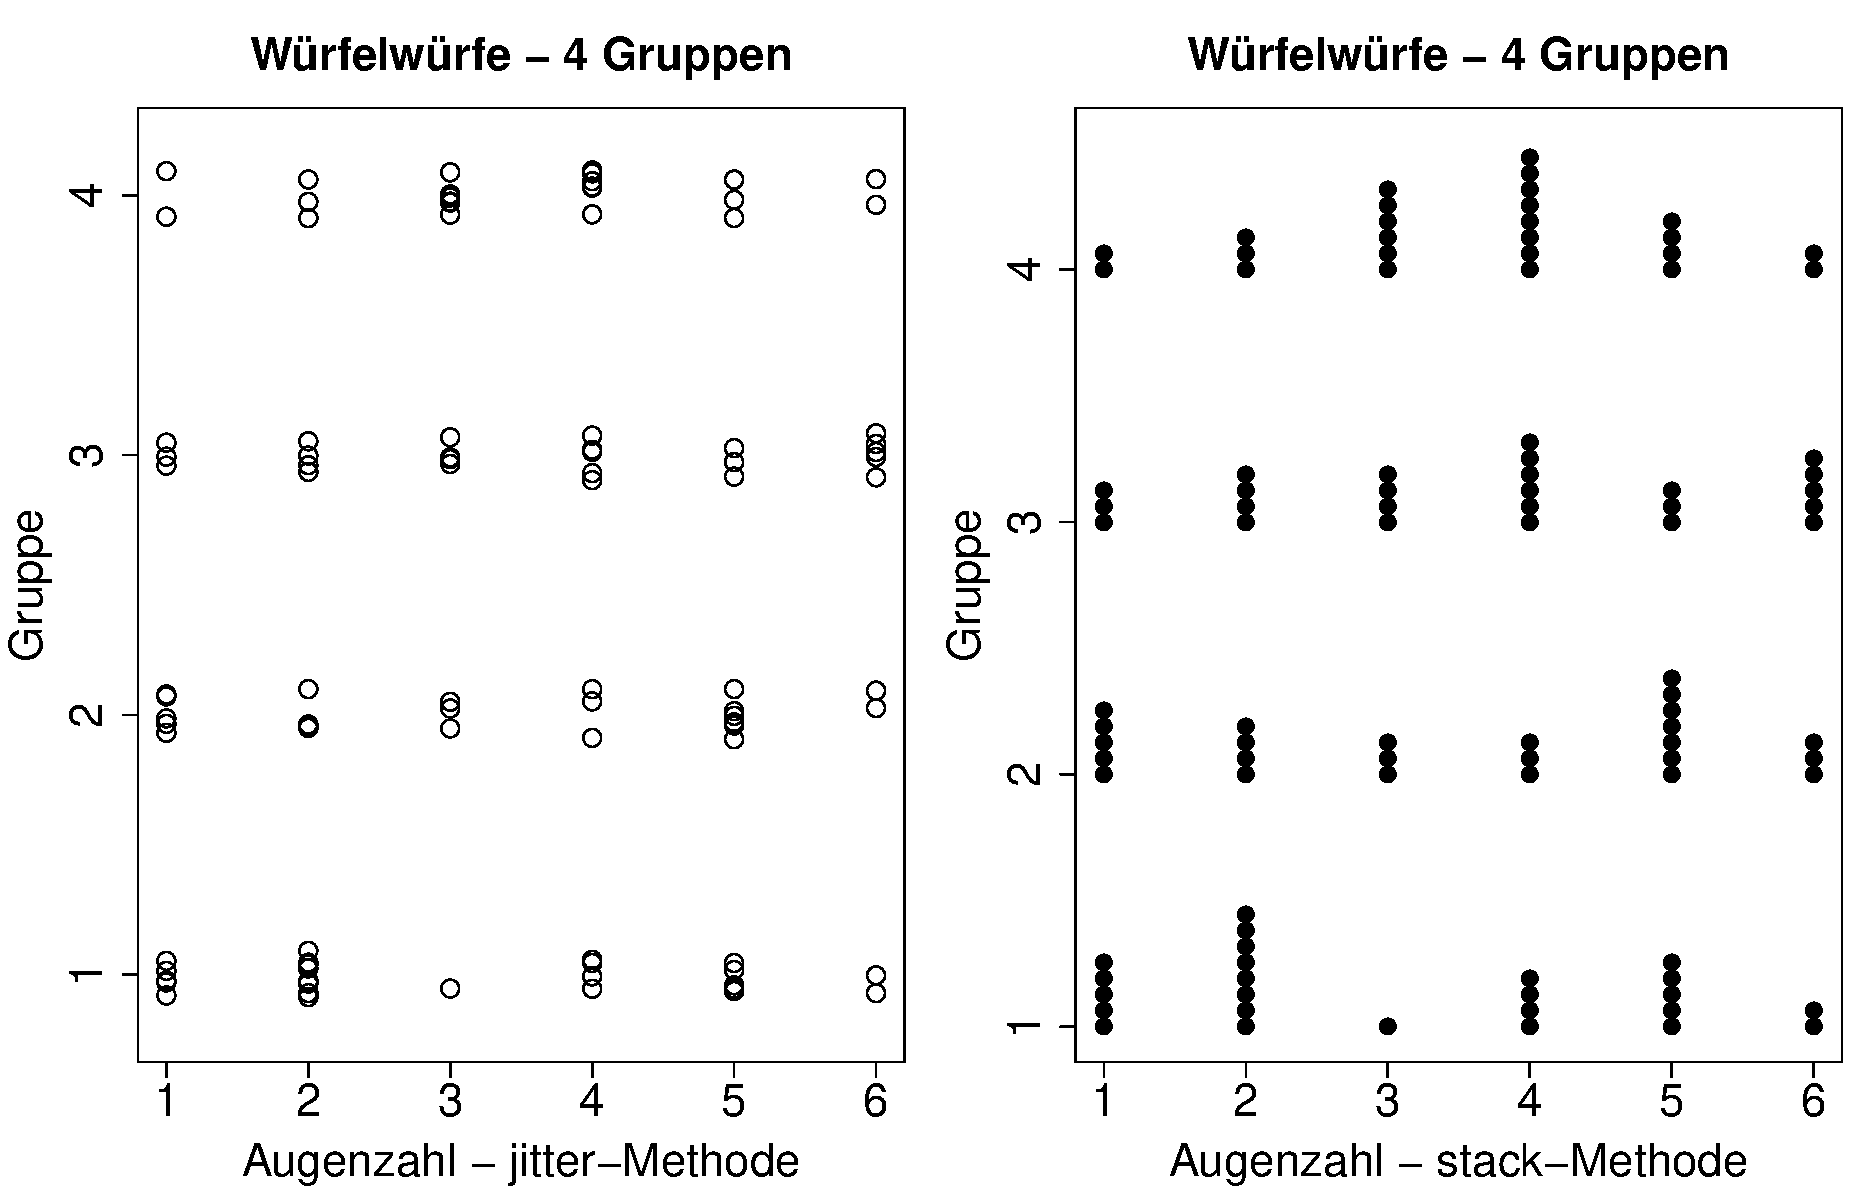
\includegraphics[width=12.5cm]{stripchart}
\vspace*{-0.5em}
\caption{Stripcharts mit verschiedenen Methoden zur Darstellung einzelner Werte}
\label{fig:stripchart}
\end{figure}

%%%%%%%%%%%%%%%%%%%%%%%%%%%%%%%%%%%%%%%%%%%%%%%%%%%%%%%%%%%%%%%%%%
%%%%%%%%%%%%%%%%%%%%%%%%%%%%%%%%%%%%%%%%%%%%%%%%%%%%%%%%%%%%%%%%%%
\subsection{Quantil-Quantil-Diagramm}
\label{sec:qq}
%%%%%%%%%%%%%%%%%%%%%%%%%%%%%%%%%%%%%%%%%%%%%%%%%%%%%%%%%%%%%%%%%%
%%%%%%%%%%%%%%%%%%%%%%%%%%%%%%%%%%%%%%%%%%%%%%%%%%%%%%%%%%%%%%%%%%

\index{Grafik!Quantil-Quantil-Diagramm}
Viele statistische Auswertungen setzen voraus, dass die zu analysierenden Variablen auf Ebene der Population eine bestimmte Verteilung aufweisen, etwa normalverteilt sind oder der Verteilung in einer anderen Population gleichen (Abschn.\ \ref{sec:modelTests}). Inwieweit die empirischen Werte mit dieser Annahme verträglich sind, kann mit einem Q-Q-Diagramm (Quantil-Quantil-Darstellung) heuristisch abgeschätzt werden.

%%%%%%%%%%%%%%%%%%%%%%%%%%%%%%%%%%%%%%%%%%%%%%%%%%%%%%%%%%%%%%%%%%
%%%%%%%%%%%%%%%%%%%%%%%%%%%%%%%%%%%%%%%%%%%%%%%%%%%%%%%%%%%%%%%%%%
\subsubsection{Vergleich zweier Stichproben}
%%%%%%%%%%%%%%%%%%%%%%%%%%%%%%%%%%%%%%%%%%%%%%%%%%%%%%%%%%%%%%%%%%
%%%%%%%%%%%%%%%%%%%%%%%%%%%%%%%%%%%%%%%%%%%%%%%%%%%%%%%%%%%%%%%%%%

Wenn die Verteilung eines Merkmals in zwei Gruppen identisch ist, stimmen auch die Quantile zu denselben Wahrscheinlichkeiten überein (Abschn.\ \ref{sec:quantFunc}). Auf empirischer Ebene lassen sich dafür die beobachteten Quantile von zwei Variablen zu denselben Wahrscheinlichkeiten in einem Diagramm gegeneinander auftragen. Sind ihre Quantile identisch, fallen die Punkte bei gleicher Achsenskalierung auf die Winkelhalbierende. Unterscheiden sich die Verteilungen lediglich durch eine lineare Transformation, fallen die Punkte auf eine Gerade. Voneinander abweichende Verteilungen werden entsprechend durch Abweichungen von einer Referenzgerade deutlich. Ein solches Diagramm erstellt\index[func]{qqplot()@\lstinline{qqplot()}} \lstinline!qqplot(x=<<Vektor>>, y=<<Vektor>>)! (Abb.\ \ref{fig:qq}). Für \lstinline!x! und \lstinline!y! sind dafür die zu vergleichenden Variablen einzutragen, die auch unterschiedliche Länge haben können.
\begin{lstlisting}
> DV1 <- rnorm(200)             # simuliere normalverteilte Messwerte 
> DV2 <- rf(100, df1=3, df2=15) # simuliere F-Verteilung, anderes N
> qqplot(DV1, DV2, xlab="Quantile N(0, 1)", ylab="Quantile F(3, 15)",
+        main="Quantile N(0, 1) vs. F(3, 15)-Verteilung", pch=19)
\end{lstlisting}

\begin{figure}[ht]
\centering
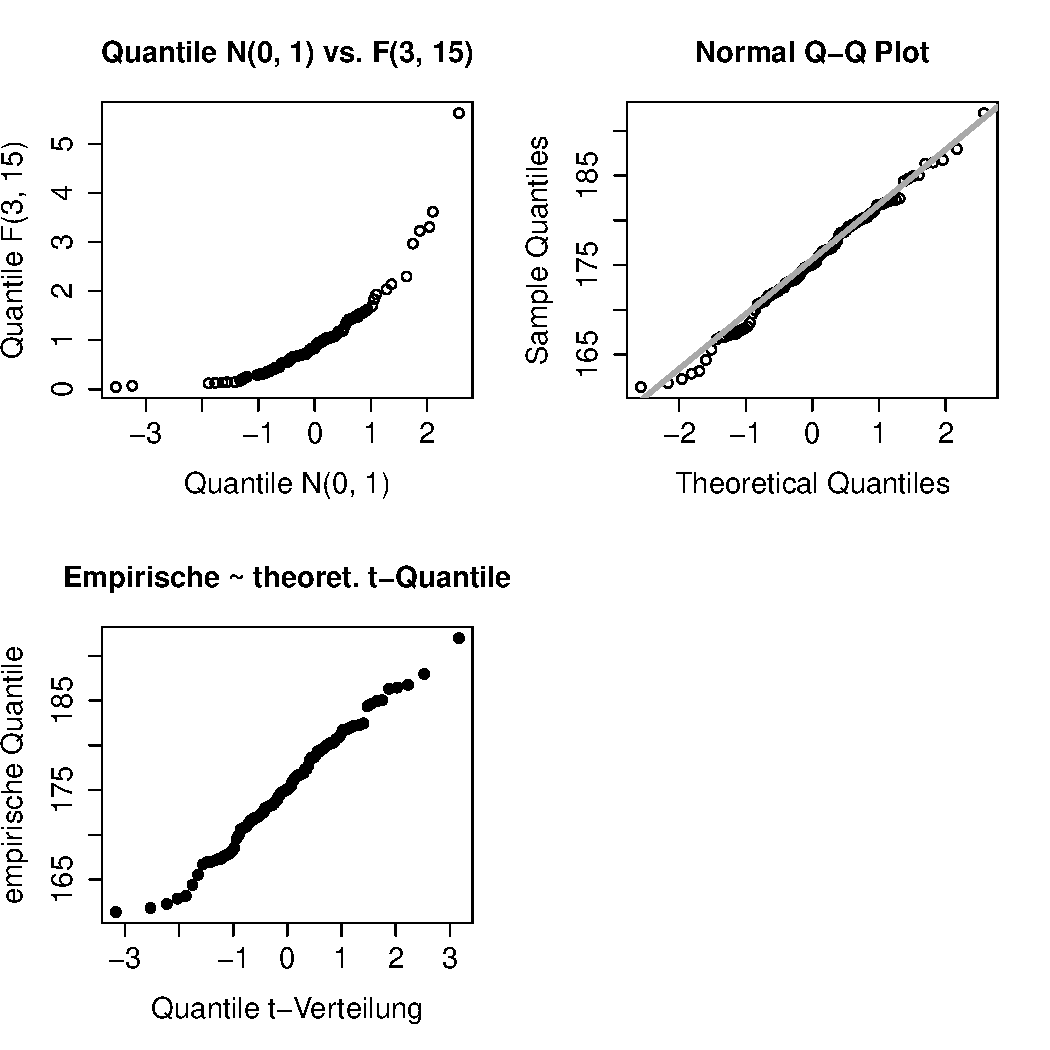
\includegraphics[width=12.5cm]{qq}
\vspace*{-0.5em}
\caption{Quantil-Quantil Darstellung zum Vergleich von zwei Stichproben, zur Überprüfung von Normalverteiltheit und zum Vergleich mit $t$-Verteilung}
\label{fig:qq}
\end{figure}

%%%%%%%%%%%%%%%%%%%%%%%%%%%%%%%%%%%%%%%%%%%%%%%%%%%%%%%%%%%%%%%%%%
%%%%%%%%%%%%%%%%%%%%%%%%%%%%%%%%%%%%%%%%%%%%%%%%%%%%%%%%%%%%%%%%%%
\subsubsection{Vergleich mit theoretischer Verteilung}
%%%%%%%%%%%%%%%%%%%%%%%%%%%%%%%%%%%%%%%%%%%%%%%%%%%%%%%%%%%%%%%%%%
%%%%%%%%%%%%%%%%%%%%%%%%%%%%%%%%%%%%%%%%%%%%%%%%%%%%%%%%%%%%%%%%%%

Die empirischen Quantile von Daten einer Stichprobe können auch mit Quantilen verglichen werden, die sich aus der Annahme einer bestimmten Verteilung ergeben. Hierfür werden die erwarteten Quantile als $x$- und die tatsächlichen Quantile als $y$-Koordinaten von Punkten in einem Streudiagramm verwendet. Die empirischen Quantile sind einfach die sortierten Werte eines Vektors. Die Funktion \lstinline!ppoints(<<Vektor>>)!\index[func]{ppoints()@\lstinline{ppoints()}} bestimmt, welches der zu einem Quantil gehörende Wert der empirischen kumulierten Häufigkeitsverteilung als Schätzung der Verteilungsfunktion ist.\footnote{Dies sind die Mittelpunkte der Intervalle, die durch die empirischen kumulierten relativen Häufigkeiten gebildet werden (Abschn.\ \ref{sec:stepfun}).} Ihre Ausgabe kann dann als Argument für die Quantilfunktion einer infrage kommenden Verteilung verwendet werden, um die theoretischen Quantile zu erhalten (Abschn.\ \ref{sec:quantFunc}). Quantile zu denselben Wahrscheinlichkeiten lassen sich dann mit \lstinline!plot()! als Streudiagramm gegeneinander auftragen.
\begin{lstlisting}
> cProb <- ppoints(height)        # kumulierte W'keit für t-Quantile
> qTheo <- qt(cProb, df=10)       # t-Quantile
> qEmp  <- sort(height)           # empirische Quantile

# Q-Q-Plot Vergleich empirische Quantile mit t-Quantilen
> plot(qTheo, qEmp, main="Empirische ~ theoretische t-Quantile",
+     xlab="Quantile t-Verteilung", ylab="empirische Quantile", pch=19)
\end{lstlisting}

Für den häufigen Spezialfall eines Vergleichs mit der Standardnormalverteilung existiert\index[func]{qqnorm()@\lstinline{qqnorm()}} \lstinline!qqnorm()!. Eine Referenzgerade wird durch\index[func]{qqline()@\lstinline{qqline()}} \lstinline!qqline()! in das Diagramm eingetragen (Abb.\ \ref{fig:qq}).
\begin{lstlisting}
qqnorm(y=<<Vektor>>, datax=FALSE)
qqline(y=<<Vektor>>, datax=FALSE)
\end{lstlisting}

Mit \lstinline!datax=FALSE! wird in der Voreinstellung festgelegt, dass die Quantile der empirischen Werte auf der $y$-Achse abgetragen werden. \lstinline!datax! ist beim Aufruf von \lstinline!qqnorm()! und \lstinline!qqline()! auf denselben Wert zu setzen. Im Vergleich zu \lstinline!qqplot()! entfällt hier die Angabe des ersten Datenvektors, da die $x$-Koordinaten der Punkte von den theoretisch erwarteten Quantilen gebildet werden.
\begin{lstlisting}
> height <- rnorm(100, mean=175, sd=7)
> qqnorm(height, pch=19)
> qqline(height, col="red", lwd=2)
\end{lstlisting}

%%%%%%%%%%%%%%%%%%%%%%%%%%%%%%%%%%%%%%%%%%%%%%%%%%%%%%%%%%%%%%%%%%
%%%%%%%%%%%%%%%%%%%%%%%%%%%%%%%%%%%%%%%%%%%%%%%%%%%%%%%%%%%%%%%%%%
\subsection{Empirische kumulierte Häufigkeitsverteilung}
\label{sec:ecdfPlot}
%%%%%%%%%%%%%%%%%%%%%%%%%%%%%%%%%%%%%%%%%%%%%%%%%%%%%%%%%%%%%%%%%%
%%%%%%%%%%%%%%%%%%%%%%%%%%%%%%%%%%%%%%%%%%%%%%%%%%%%%%%%%%%%%%%%%%

\index{Grafik!kumulierte Häufigkeiten}
Die kumulierte Häufigkeitsverteilung empirischer Daten lässt sich durch die\index[func]{ecdf()@\lstinline{ecdf()}} \lstinline!ecdf()! Funktion ermitteln, die ihrerseits eine Funktion erzeugt (Abschn.\ \ref{sec:stepfun}). Zur grafischen Darstellung wird diese neue Funktion an \lstinline!plot()! übergeben (Abb.\ \ref{fig:ecdf}).
\begin{lstlisting}
> vec <- round(rnorm(10), 1)
> Fn  <- ecdf(vec)
> plot(Fn, main="Empirische kumulierte Häufigkeitsverteilung")
> curve(pnorm, add=TRUE, col="gray", lwd=2) # Vergleich mit Standard-NV
\end{lstlisting}

\begin{figure}[ht]
\centering
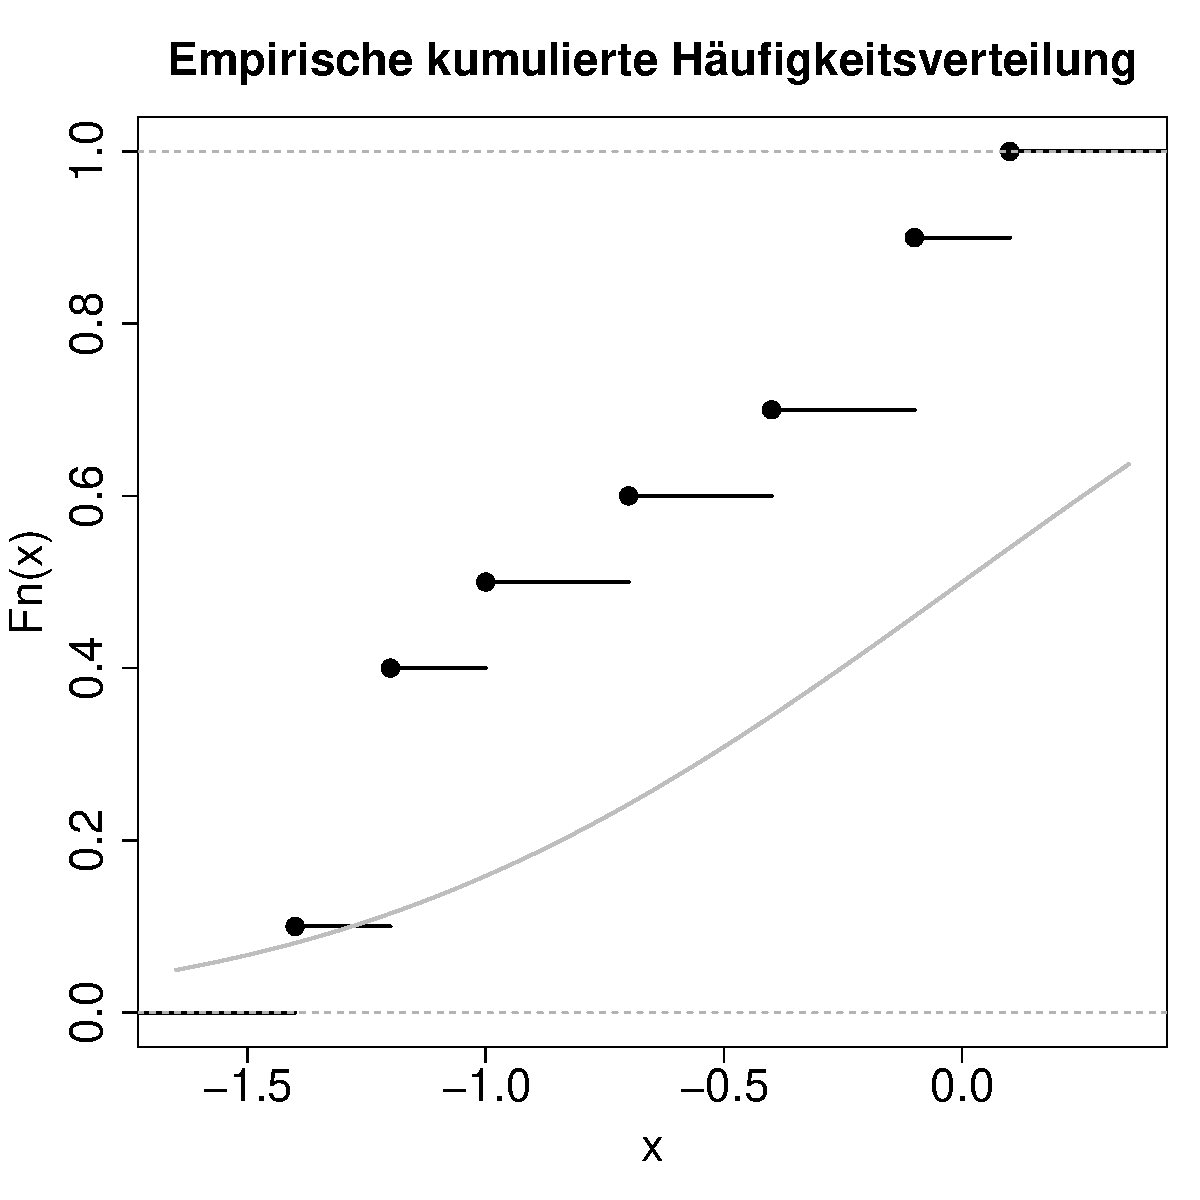
\includegraphics[width=8cm]{ecdf}
\vspace*{-1em}
\caption{Vergleich von empirischen kumulierten Häufigkeiten mit der Verteilungsfunktion der Standardnormalverteilung}
\label{fig:ecdf}
\end{figure}

%%%%%%%%%%%%%%%%%%%%%%%%%%%%%%%%%%%%%%%%%%%%%%%%%%%%%%%%%%%%%%%%%%
%%%%%%%%%%%%%%%%%%%%%%%%%%%%%%%%%%%%%%%%%%%%%%%%%%%%%%%%%%%%%%%%%%
\subsection{Kreisdiagramm}
%%%%%%%%%%%%%%%%%%%%%%%%%%%%%%%%%%%%%%%%%%%%%%%%%%%%%%%%%%%%%%%%%%
%%%%%%%%%%%%%%%%%%%%%%%%%%%%%%%%%%%%%%%%%%%%%%%%%%%%%%%%%%%%%%%%%%

\index{Grafik!Kreisdiagramm}
Das Kreis- oder auch Tortendiagramm ist eine weitere Möglichkeit, die Werte einer diskreten Variable grob zu veranschaulichen. Hier repräsentiert die Größe eines farblich hervorgehobenen Kreissektors den Anteil des zugehörigen Wertes an der Summe aller Werte. Da die korrekte Einschätzung von Flächeninhalten bzw.\ Sektorgrößen deutlich schwerer fällt als etwa der Vergleich von Linienlängen, sind Kreisdiagramme oft schlecht ablesbar und werden daher nicht häufig im wissenschaftlichen Kontext verwendet\index[func]{pie()@\lstinline{pie()}} (Abb.\ \ref{fig:pie}).
\begin{lstlisting}
pie(x=<<Vektor>>, labels="<<Namen>>", col="<<Farben>>")
\end{lstlisting}

Für \lstinline!x! ist ein Datenvektor mit nicht negativen Werten anzugeben. Sollen die einzelnen Sektoren mit einer Bezeichnung versehen werden, kann ein Vektor aus entsprechenden Zeichenketten für das Argument \lstinline!labels! übergeben werden. Das Argument \lstinline!col! kontrolliert die Farbe der Sektoren.
\begin{lstlisting}
> dice <- sample(1:6, 100, replace=TRUE)    # Würfelwürfe
> dTab <- table(dice)                       # absolute Häufigkeiten
> pie(dTab, col=c("blue", "red", "yellow", "pink", "green", "orange"),
+     main="Relative Häufigkeiten beim Würfeln")
\end{lstlisting}

Um die Kreissektoren zu beschriften, wird hier \lstinline!text()! verwendet. Die zur Plazierung notwendigen $(x, y)$-Koordinaten ergeben sich aus den relativen Häufigkeiten der Würfelergebnisse. Dabei ist dafür zu sorgen, dass die Beschriftung immer in der Mitte eines Sektors liegt. Die Kreismitte hat die Koordinaten $(0, 0)$, der Radius des Kreises beträgt $1$. Die Beschriftungen liegen mit ihrem Mittelpunkt also auf einem Kreis mit Radius $0.5$.
\begin{lstlisting}
> dTabFreq <- proportions(dTab)             # relative Häufigkeiten
> textRad  <- 0.5                           # Radius für Beschriftungen
> angles   <- dTabFreq * 2 * pi             # Sektorgrößen als Winkel
> csAngles <- cumsum(angles)                # Winkel der Sektorgrenzen
> csAngles <- csAngles - angles/2           # Winkel der Sektormitten
> textX    <- textRad * cos(csAngles)       # x-Koordinaten für Text
> textY    <- textRad * sin(csAngles)       # y-Koordinaten für Text
> text(x=textX, y=textY, labels=dTabFreq)   # Sektorbeschriftungen
\end{lstlisting}

\begin{figure}[ht]
\centering
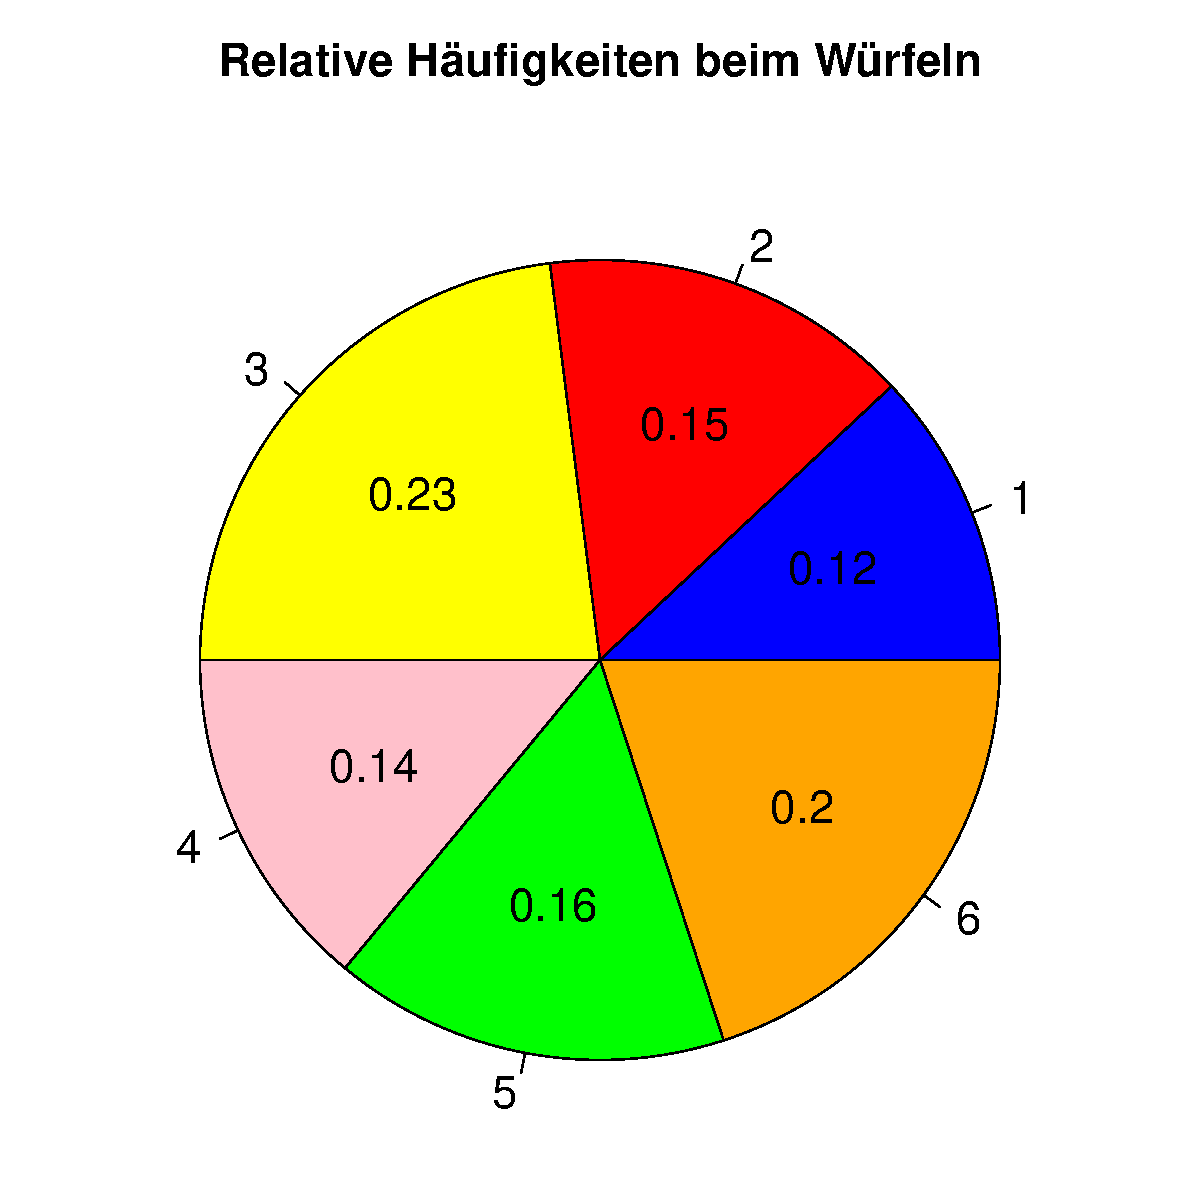
\includegraphics[width=8cm]{pie}
\vspace*{-1.5em}
\caption{Kreisdiagramm als Mittel zur Darstellung von Kategorienhäufigkeiten}
\label{fig:pie}
\end{figure}

%%%%%%%%%%%%%%%%%%%%%%%%%%%%%%%%%%%%%%%%%%%%%%%%%%%%%%%%%%%%%%%%%%
%%%%%%%%%%%%%%%%%%%%%%%%%%%%%%%%%%%%%%%%%%%%%%%%%%%%%%%%%%%%%%%%%%
\subsection{Gemeinsame Verteilung zweier Variablen}
\label{sec:distr2var}
%%%%%%%%%%%%%%%%%%%%%%%%%%%%%%%%%%%%%%%%%%%%%%%%%%%%%%%%%%%%%%%%%%
%%%%%%%%%%%%%%%%%%%%%%%%%%%%%%%%%%%%%%%%%%%%%%%%%%%%%%%%%%%%%%%%%%

\index{Grafik!gemeinsame Verteilung}
\index{Grafik!Streuungsellipse}
\index{Streuungsellipse|see{Grafik}}
Die in Abschn.\ \ref{sec:plot} vorgestellte \lstinline!plot()! Funktion eignet sich dafür, die gemeinsame Verteilung von zwei Variablen in Form eines Streudiagramms zu untersuchen. Stammen die Daten aus verschiedenen Gruppen, kann die Gruppenzugehörigkeit über die Farbe oder den Typ der Datenpunktsymbole gekennzeichnet werden. Hierfür lässt sich die Eigenschaft von Faktoren ausnutzen, dass ihre Stufen intern über natürliche Zahlen repräsentiert sind, die sich mit \lstinline!unclass()! ausgeben lassen und damit als Indizes dienen können (Abb.\ \ref{fig:distr2var}).
\begin{lstlisting}
> N  <- 200                                 # Anzahl Personen
> P  <- 2                                   # Anzahl Gruppen
> x  <- rnorm(N, 100, 15)                   # Daten Variable 1
> y  <- 0.5*x + rnorm(N, 0, 10)             # Daten Variable 2
> IV <- gl(P, N/P, labels=LETTERS[1:P])     # Gruppierungsfaktor

# gemeinsame Verteilung mit 2 Datenpunktsymbolen und Legende
> plot(x, y, pch=c(4, 16)[unclass(IV)], lwd=2,
+      col=c("black", "darkgray")[unclass(IV)],
+      main="Gemeinsame Verteilung je Gruppe")

> legend(x="topleft", legend=c("Gruppe A", "Gruppe B"),
+        pch=c(4, 16), col=c("black", "darkgray"))
\end{lstlisting}

Weiterhin kann es hilfreich sein, mit \lstinline!ellipse()! \index[func]{ellipse()@\lstinline{ellipse()}} aus dem Paket\index[pack]{car@\lstinline{car}} \lstinline!car! auch die Streuungsellipse der gemeinsamen Verteilung einzuzeichnen, wie sie durch die Eigenwerte und Eigenvektoren der Kovarianzmatrix der Variablen definiert wird (Abschn.\ \ref{sec:matProp}, \ref{sec:multPCA}).\footnote{Für Konfidenzellipsen im inferenzstatistischen Sinn s.\ \lstinline!confidenceEllipse()! \index[func]{confidenceEllipse()@\lstinline{confidenceEllipse()}} aus demselben Paket.}
\begin{lstlisting}
ellipse(<<Zentroid>>, shape=<<Kovarianzmatrix>>, radius=<<Radius>>)
\end{lstlisting}

Die Ellipse hat ihren Mittelpunkt im als ersten Argument zu übergebendem Zentroid der Daten. Die Hauptachsen sind durch die Eigenvektoren der für \lstinline!shape! zu nennenden Matrix gegeben, wobei die Länge jeder Halbachse gleich der Wurzel aus dem zugehörigen Eigenwert ist (Abb. \ref{fig:distr2var}). Mit \lstinline!radius! kann diese Länge um einen beliebigen Faktor skaliert werden.
\begin{lstlisting}
> library(car)                                  # für ellipse()
> mat <- cbind(x, y)                            # Datenmatrix
> ctr <- colMeans(mat)                          # Zentroid
> plot(mat, xlab="x", ylab="y", asp=1,          # gemeinsame Verteilung
+      main="Gemeinsame Verteilung 2 Variablen")

> ellipse(ctr, shape=cov(mat), radius=1, col="blue") # Streuungsellipse
\end{lstlisting}

\begin{figure}[ht]
\centering
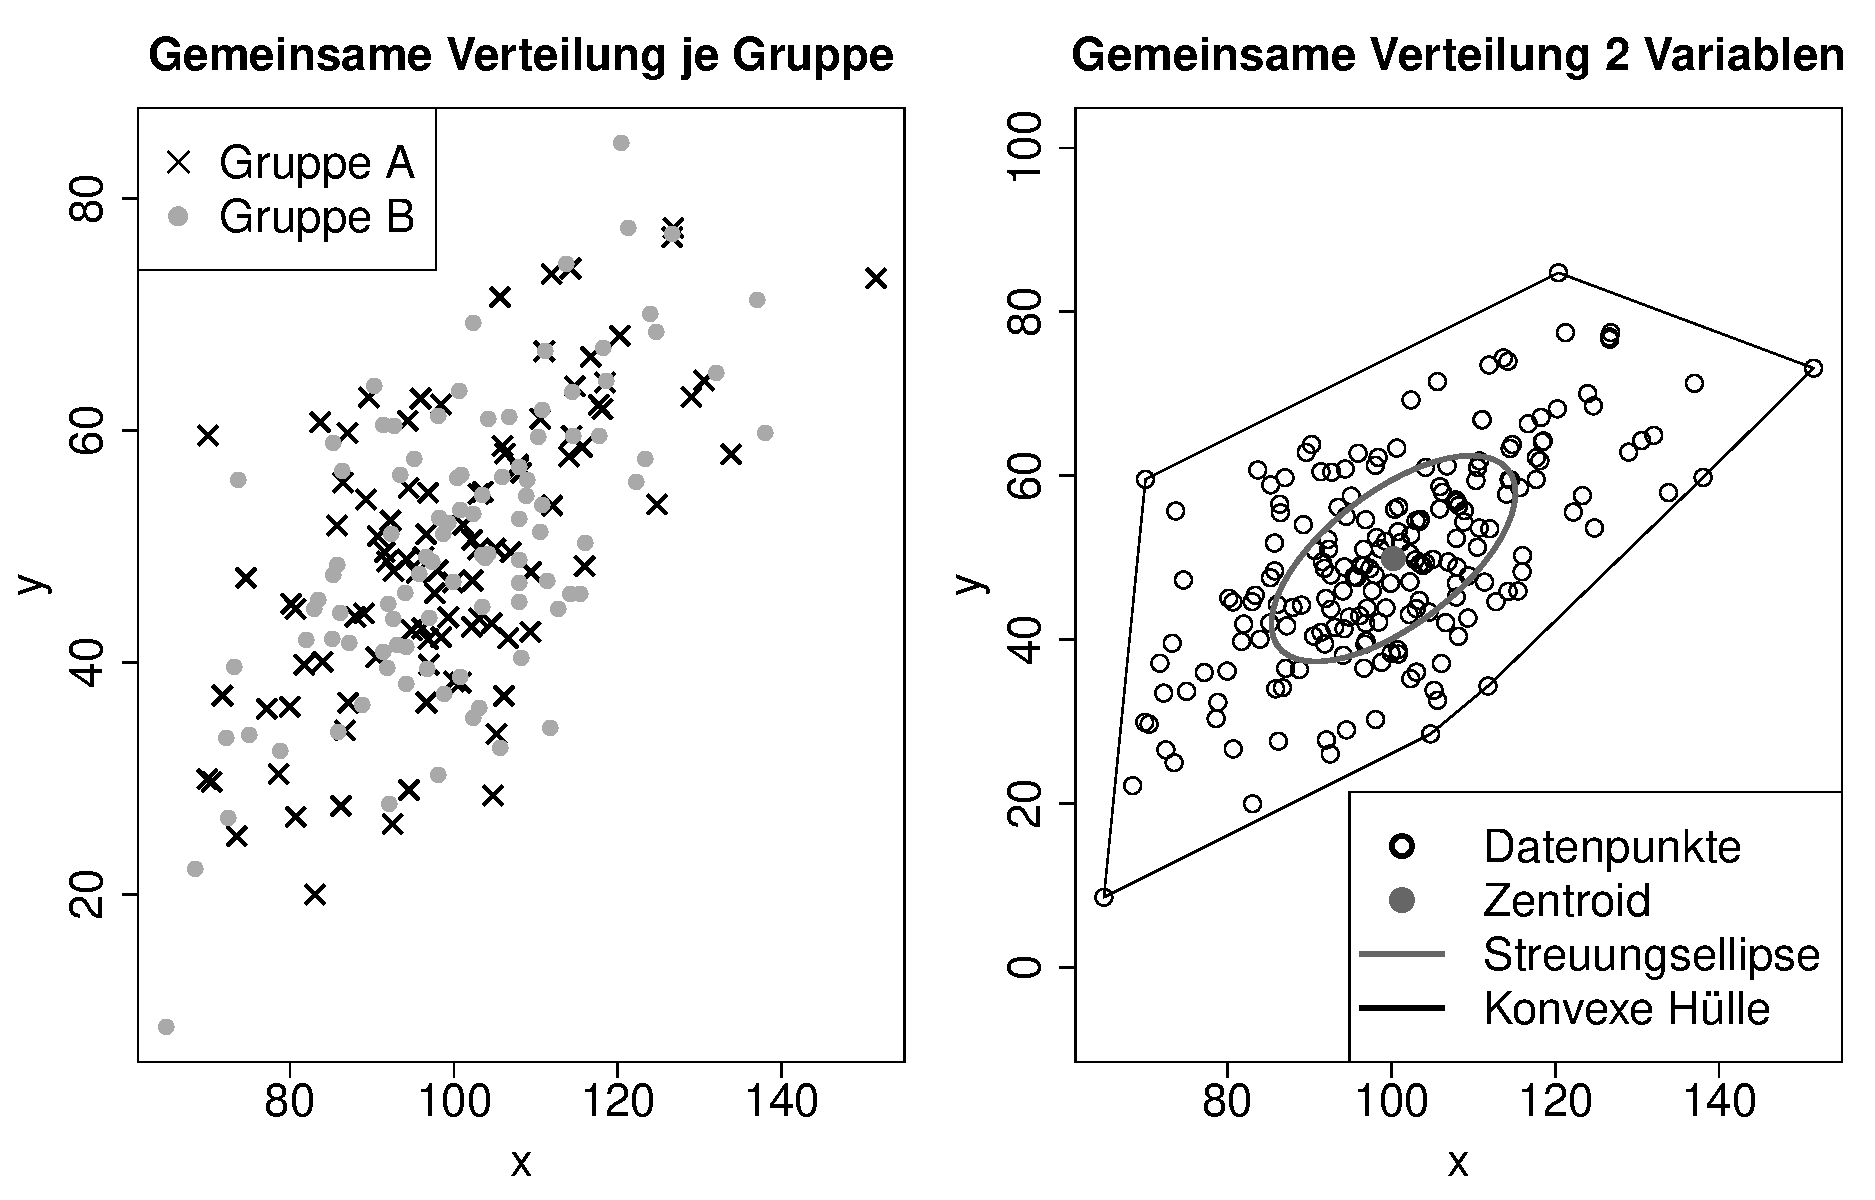
\includegraphics[width=12.5cm]{distr2var}
\vspace*{-1em}
\caption{Gemeinsame Verteilung zweier Variablen getrennt nach Gruppen. Gesamtdaten mit Streuungsellipse, deren Hauptachsen und der konvexen Hülle}
\label{fig:distr2var}
\end{figure}

\index{Grafik!konvexe Hülle}
\index{konvexe Hülle|see{Grafik}}
\index{Daten!Ausreißer}
Die konvexe Hülle der gemeinsamen Verteilung zweier Variablen ist definiert als kleinstes konvexes Polygon, in dem, bzw.\ auf dessen Rand alle Datenpunkte liegen. Ihr mit\index[func]{chull()@\lstinline{chull()}} \lstinline!chull()! ermittelbarer Rand markiert die extremsten Datenpunkte der Verteilung und kann damit bei der Identifikation von Ausreißern hilfreich sein (Abb. \ref{fig:distr2var}).
\begin{lstlisting}
chull(x=<<Vektor>>, y=<<Vektor>>)
\end{lstlisting}

Unter \lstinline!x! und \lstinline!y! sind die Ausprägungen der ersten und zweiten Variable jeweils als Vektor einzutragen. Wird nur ein Vektor angegeben, werden seine Elemente als $y$-Koordinaten interpretiert und die $x$-Koordinate jedes Datenpunkts gleich dem Index des zugehörigen Vektorelements gesetzt. Die Ausgabe liefert im Uhrzeigersinn die Indizes der Ecken des Polygons.
\begin{lstlisting}
> hullIdx <- chull(x, y)                  # Indizes Ecken konvexe Hülle
> polygon(x[hullIdx], y[hullIdx])         # konvexe Hülle einzeichnen
> legend(x="bottomright", legend=c("Datenpunkte", "Zentroid",
+        "Streuungsellipse", "konvexe Hülle"),
+        pch=c(1, 19, NA, NA), lty=c(NA, NA, 1, 1),
+        col=c("black", "blue", "blue", "black"))
\end{lstlisting}

\label{sec:plotManyValsA}
Sind nur wenige Wertepaare möglich und deswegen Bindungen in den Daten vorhanden, würden mehrere gleiche Wertepaare durch dasselbe Symbol im Diagramm dargestellt. Sollen dagegen unter Verzicht auf die präzise Positionierung ebenso viele Symbole wie Wertepaare angezeigt werden, kann dies mit\index[func]{jitter()@\lstinline{jitter()}} \lstinline!jitter(<<Variable>>)! erreicht werden. Diese Funktion ändert die Werte der Variable um einen kleinen zufälligen Betrag und bewirkt dadurch beim Zeichnen jedes Datenpunkts einen zufälligen Versatz entlang der zugehörigen Achse (Abb.\ \ref{fig:plotJitter}).
\begin{lstlisting}
> vec1 <- sample(1:10, 100, replace=TRUE)
> vec2 <- sample(1:10, 100, replace=TRUE)
> plot(vec2 ~ vec1, main="Punktwolke")    # Datenpunkte ohne jitter()

# Datenpunkte: zufälliger Versatz entlang y-Achse durch jitter()
> plot(jitter(vec2) ~ vec1, main="Punktwolke mit jitter")
\end{lstlisting}

\begin{figure}[ht]
\centering
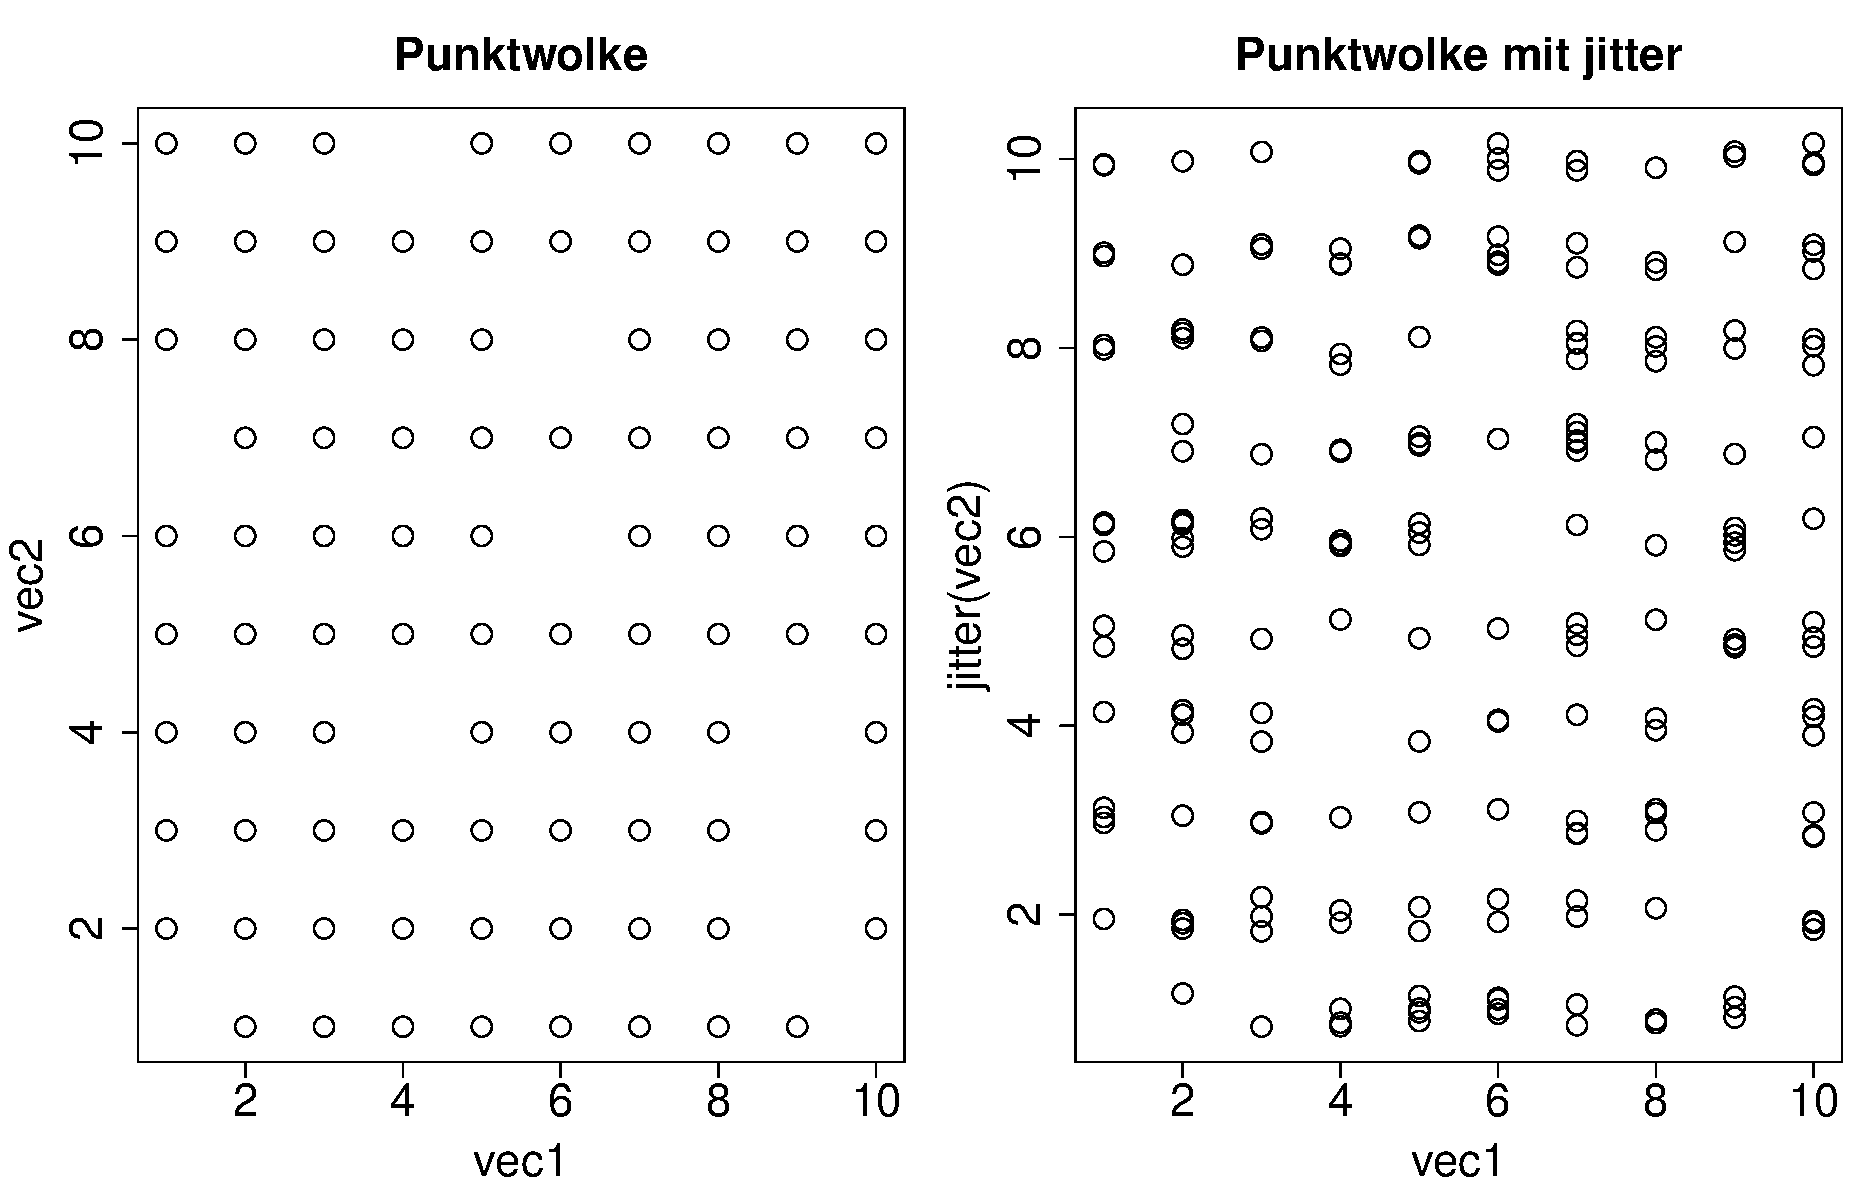
\includegraphics[width=12.5cm]{plotJitter}
\vspace*{-1em}
\caption{Streudiagramm von Daten mit Bindungen ohne und mit Anwendung von \lstinline!jitter()!}
\label{fig:plotJitter}
\end{figure}

Bei sehr vielen darzustellenden Punkten taucht mitunter das Problem auf, dass Datenpunktsymbole einander überdecken und einzelne Werte nicht mehr identifizierbar sind. Indem als Datenpunktsymbol mit \lstinline!pch="."! der Punkt gewählt wird, lässt sich dies bis zu einem gewissen Grad verhindern. Auch der Einsatz von simulierter Transparenz für die Datenpunktsymbole kann einzelne Werte identifizierbar halten: Bei einer sehr durchlässig gewählten Farbe erzeugt ein einzelner Datenpunkt nur einen schwachen Abdruck, während viele aufeinander liegende Punkte die Farbe an dieser Stelle des Diagramms immer gesättigter machen (Abschn.\ \ref{sec:colors}, Fußnote \ref{ftn:transp}).

Alternativ lässt sich mit\index[func]{hexbin()@\lstinline{hexbin()}} \lstinline!hexbin()! aus dem gleichnamigen\index[pack]{hexbin@\lstinline{hexbin}} Paket \cite{Carr2009} ein Diagramm erstellen, das die Diagrammfläche in hexagonale Regionen einteilt und die Dichte der Datenpunkte in jeder Region ähnlich einem Höhenlinien-Diagramm (Abschn.\ \ref{sec:3dContour}) farblich repräsentiert. Auch\index[func]{smoothScatter()@\lstinline{smoothScatter()}} \lstinline!smoothScatter()! codiert die Dichte von Datenpunkten über farblich abgesetzte Diagrammregionen, verwendet dabei jedoch einen 2D-Kerndichteschätzer zur Glättung der Regionengrenzen (Abschn.\ \ref{sec:density}).

%%%%%%%%%%%%%%%%%%%%%%%%%%%%%%%%%%%%%%%%%%%%%%%%%%%%%%%%%%%%%%%%%%
%%%%%%%%%%%%%%%%%%%%%%%%%%%%%%%%%%%%%%%%%%%%%%%%%%%%%%%%%%%%%%%%%%
\section{Multivariate Daten visualisieren}
\label{sec:3dPlot}
%%%%%%%%%%%%%%%%%%%%%%%%%%%%%%%%%%%%%%%%%%%%%%%%%%%%%%%%%%%%%%%%%%
%%%%%%%%%%%%%%%%%%%%%%%%%%%%%%%%%%%%%%%%%%%%%%%%%%%%%%%%%%%%%%%%%%

\index{Grafik!multivariate Daten}
\index{Grafik!3D}
In unterschiedlichen Situationen kann es erstrebenswert sein, multivariate Daten grafisch darzustellen: So können Messwerte in ihrer Ausprägung von mehr als einer numerischen Variable abhängen, etwa im Kontext einer multiplen linearen Regression. Oder aber mehrere Variablen werden gleichzeitig erhoben, um ihre gemeinsame Verteilung zu analysieren. Schließlich hängt etwa im Rahmen mehrfaktorieller Varianzanalysen eine Variable von der Kombination verschiedener qualitativer Faktoren ab. Die Visualisierung solcher Daten muss dann alle beteiligten Komponenten berücksichtigen. Da Diagramme nur zweidimensional sein können, ergibt sich dabei das Problem, dass die räumliche Lage eines Datenpunkts in der Plot-Region nicht mehr als zwei Komponenten repräsentieren kann.

Für dreidimensionale Daten existieren als Ausweg verschiedene Diagrammtypen, die sich darin unterscheiden, auf welche Weise die dritte Komponente grafisch codiert wird: So wird versucht, einen räumlichen Tiefeneindruck zu erzeugen und die dritte Komponente als $z$-Koordinate, d.\,h.\ als Höhe eines Datenpunkts über einer Ebene zu repräsentieren (dreidimensionale Streudiagramme und Gitterflächen). Oder die dritte Komponente wird nicht räumlich, sondern farblich bzw.\ durch andere grafische Unterscheidungsmerkmale symbolisiert, etwa durch Höhenlinien oder die Größe der Datenpunktsymbole. Bei mehr als drei Variablen kann auf die direkte Veranschaulichung aller Komponenten zugunsten einer aufgeteilten Grafik verzichtet werden, in der eine Serie uni- oder bivariater Diagramme nebeneinander für alle Stufen bzw.\ Stufenkombinationen weiterer Variablen angeordnet ist.

%%%%%%%%%%%%%%%%%%%%%%%%%%%%%%%%%%%%%%%%%%%%%%%%%%%%%%%%%%%%%%%%%%
%%%%%%%%%%%%%%%%%%%%%%%%%%%%%%%%%%%%%%%%%%%%%%%%%%%%%%%%%%%%%%%%%%
\subsection{Höhenlinien und variable Datenpunktsymbole}
\label{sec:3dContour}
%%%%%%%%%%%%%%%%%%%%%%%%%%%%%%%%%%%%%%%%%%%%%%%%%%%%%%%%%%%%%%%%%%
%%%%%%%%%%%%%%%%%%%%%%%%%%%%%%%%%%%%%%%%%%%%%%%%%%%%%%%%%%%%%%%%%%

\index{Grafik!Höhenlinien}
Den Diagrammtypen, die Höhenlinien oder Gitter zur Visualisierung der $z$-Koordinate verwenden, ist die Art der Angabe von Koordinaten gemein. Sie benötigen zum einen zwei Vektoren, die die Werte auf der $x$- und $y$-Achse festlegen. Als drittes Argument erwarten die Funktionen eine Matrix, die Werte für jede Kombination der übergebenen $(x, y)$-Koordinaten enthält und deswegen so viele Zeilen wie $x$- und so viele Spalten wie $y$-Koordinaten besitzt. Die Werte dieser Matrix definieren die $z$-Koordinate als dritte Komponente für jedes $(x, y)$-Koordinatenpaar.

Höhenlinien symbolisieren die $z$-Koordinate wie topografische Karten durch die Zugehörigkeit eines Punkts zu einer Region der Diagrammfläche, die durch eine geschlossene Höhenlinie definiert wird. Dieses Vorgehen ist mit einer Vergröberung der Daten verbunden, da Wertebereiche in Kategorien zusammengefasst\index[func]{contour()@\lstinline{contour()}} werden.
\begin{lstlisting}
contour(x=<<x-Koordinaten>>, y=<<y-Koordinaten>>, z=<<z-Koordinaten>>,
        nlevels=<<Anzahl Höhenlinien>>, levels=<<Kategorien>>,
        labels="<<Namen>>", drawlabels=TRUE)
\end{lstlisting}

Für \lstinline!x! und \lstinline!y! muss jeweils ein Vektor mit den $x$- bzw.\ $y$-Koordinaten der Datenpunkte übergeben werden. Die Matrix \lstinline!z! definiert die $z$-Koordinaten in der o.\,g.\ Form. Welche Kategorien Verwendung finden, kann über die Argumente \lstinline!levels! und \lstinline!nlevels! kontrolliert werden. Für \lstinline!levels! ist ein Vektor aus Kategorienbezeichnungen zu übergeben. In diesem Fall ist die Verwendung von \lstinline!nlevels! nicht mehr notwendig, da sich die Zahl der Kategorien aus der Länge von \lstinline!levels! ergibt. Andernfalls ist für \lstinline!nlevels! die gewünschte Anzahl an Kategorien zu nennen. Das Argument \lstinline!drawlabels! bestimmt, ob die Kategorienbezeichnungen im Diagramm eingetragen werden.

Im folgenden Beispiel soll die Dichtefunktion von zwei gemeinsam normalverteilten Variablen mit positiver Korrelation dargestellt werden (Abb.\ \ref{fig:3dOne}). Um die Dichte zu berechnen, wird zunächst eine eigene Funktion definiert (Abschn.\ \ref{sec:function}), die \lstinline!dmvnorm()!\index[func]{dmvnorm()@\lstinline{dmvnorm()}} aus dem\index[pack]{mvtnorm@\lstinline{mvtnorm}} \lstinline!mvtnorm! Paket für ein $(x, y)$-Koordinatenpaar aufruft. Mit \lstinline!outer()! lässt sich die Funktion dann auf alle Paare von $(x, y)$-Koordinaten anwenden.
\begin{lstlisting}
> mu    <- c(1, 3)             # Erwartungswerte Normalverteilung
> sigma <- matrix(c(1, 0.6, 0.6, 1), nrow=2)          # Kovarianzmatrix
> rng   <- 2.5                 # Wertebereich in Std.-Abw.
> N     <- 50                  # Anzahl der x- und der y-Koordinaten

# x- und y-Koordinaten
> X <- seq(from=mu[1] - rng*sigma[1, 1],
+          to=mu[1]   + rng*sigma[1, 1], length.out=N)

> Y <- seq(from=mu[2] - rng*sigma[2, 2],
+          to=mu[2]   + rng*sigma[2, 2], length.out=N)

# Funktion, um Dichte z für gegebenes (x, y)-Paar zu erzeugen
> library(mvtnorm)                                    # für dmvnorm()
> genZ <- function(x, y) { dmvnorm(cbind(x, y), mu, sigma) }

# Dichte z für alle (x, y)-Koordinatenpaare berechnen
> matZ <- outer(X, Y, "genZ")
> contour(X, Y, matZ, main="Höhenlinien für 2D-NV Dichte")
\end{lstlisting}

\index{Grafik!Höhenlinien}
Die durch die Höhenlinien definierten Regionen können mit\index[func]{filled.contour()@\lstinline{filled.contour()}} \lstinline!filled.contour()! auch eingefärbt werden. Dabei stammen die Farben aus einem Farbverlauf, dessen Zuordnung zu Kategorien auf der rechten Seite des Diagramms in einer Legende erläutert wird (Abb.\ \ref{fig:3dOne}). Der Aufruf gleicht dem für \lstinline!contour()! stark, jedoch kann über das zusätzliche Argument \lstinline!color.palette! eine andere Farbpalette spezifiziert werden (Abschn.\ \ref{sec:colors}).
\begin{lstlisting}
> filled.contour(X, Y, matZ, main="Farbige Höhenlinien")
\end{lstlisting}

Mit\index[func]{symbols()@\lstinline{symbols()}} \lstinline!symbols()! lassen sich zwei -- typischerweise quantitative -- Variablen durch die räumliche Lage von Datenpunktsymbolen gemeinsam mit weiteren Variablen durch die Gestaltung dieser Symbole grafisch repräsentieren (Abb.\ \ref{fig:3dOne}).\footnote{Ähnliche Abbildungen erzeugen\index[func]{stars()@\lstinline{stars()}} \lstinline!stars()! und\index[func]{sunflowerplot()@\lstinline{sunflowerplot()}} \lstinline!sunflowerplot()!.}
\begin{lstlisting}
symbols(x=<<Vektor>>, y=<<Vektor>>, add=FALSE, circles=<<Vektor>>,
        boxplots=<<Nx5 Matrix>>, inch=TRUE,
        fg="<<Farben>>", bg="<<Farben>>")

\end{lstlisting}

Für \lstinline!x! und \lstinline!y! muss jeweils ein Vektor mit den $x$- bzw.\ $y$-Koordinaten der Datenpunkte genannt werden, alternativ ist auch eine Modellformel der Form \lstinline!<<y>> ~ <<x>>! möglich. Welche Datenpunktsymbole an diesen Koordinaten erscheinen, richtet sich danach, für welches weitere Argument Daten übergeben werden: \lstinline!circles! erwartet einen Vektor derselben Länge wie \lstinline!x! und \lstinline!y! mit positiven Werten für die Größe der als Datenpunktsymbol dienenden Kreise. Der größte Wert entspricht in der Voreinstellung \lstinline!inch=TRUE! einer Symbolgröße von 1~in, die Größe der übrigen Symbole richtet sich nach dem Verhältnis der zugehörigen Werte zum Maximum. Wird an \lstinline!inch! stattdessen ein numerischer Wert übergeben, definiert er die Maximalgröße der Symbole. Um an jedem Koordinatenpaar einen boxplot zu zeichnen, muss an \lstinline!boxplots! eine Matrix mit $5$ Spalten und so vielen Zeilen übergeben werden, wie \lstinline!x! und \lstinline!y! jeweils Elemente besitzen. Die Werte in den Spalten stehen dabei für die Breite und Höhe der Boxen, für die Länge der unteren und oberen Striche (whiskers) sowie für den Median. Für weitere Symbole vgl.\ \lstinline!?symbols!. Die Farben der Symbole legt \lstinline!fg!, die der von ihnen umschlossenen Flächen \lstinline!bg! fest.

Das Beispiel soll anhand eines (sicher unrealistischen) Modells den Zusammenhang zwischen den negativ korrelierten Prädiktoren Alter und Sport (in Minuten pro Woche) und dem Körpergewicht als gemessene Variable simulieren.
\begin{lstlisting}
> N      <- 10
> age    <- rnorm(N, 30, 8)
> sport  <- abs(-0.25*age + rnorm(N, 60, 30))
> weight <- -0.3*age -0.4*sport + 100 + rnorm(N, 0, 3)

# reskaliere Werte für das Körpergewicht auf das Intervall [0.2, 1]
> wScale <- (weight-min(weight)) * (0.8 / abs(diff(range(weight))))+0.2
> symbols(age, sport, circles=wScale, inch=0.6, fg=NULL, bg=rainbow(N),
+         main="Gewicht vs. Alter und Sport")

\end{lstlisting}

\begin{figure}[ht]
\centering

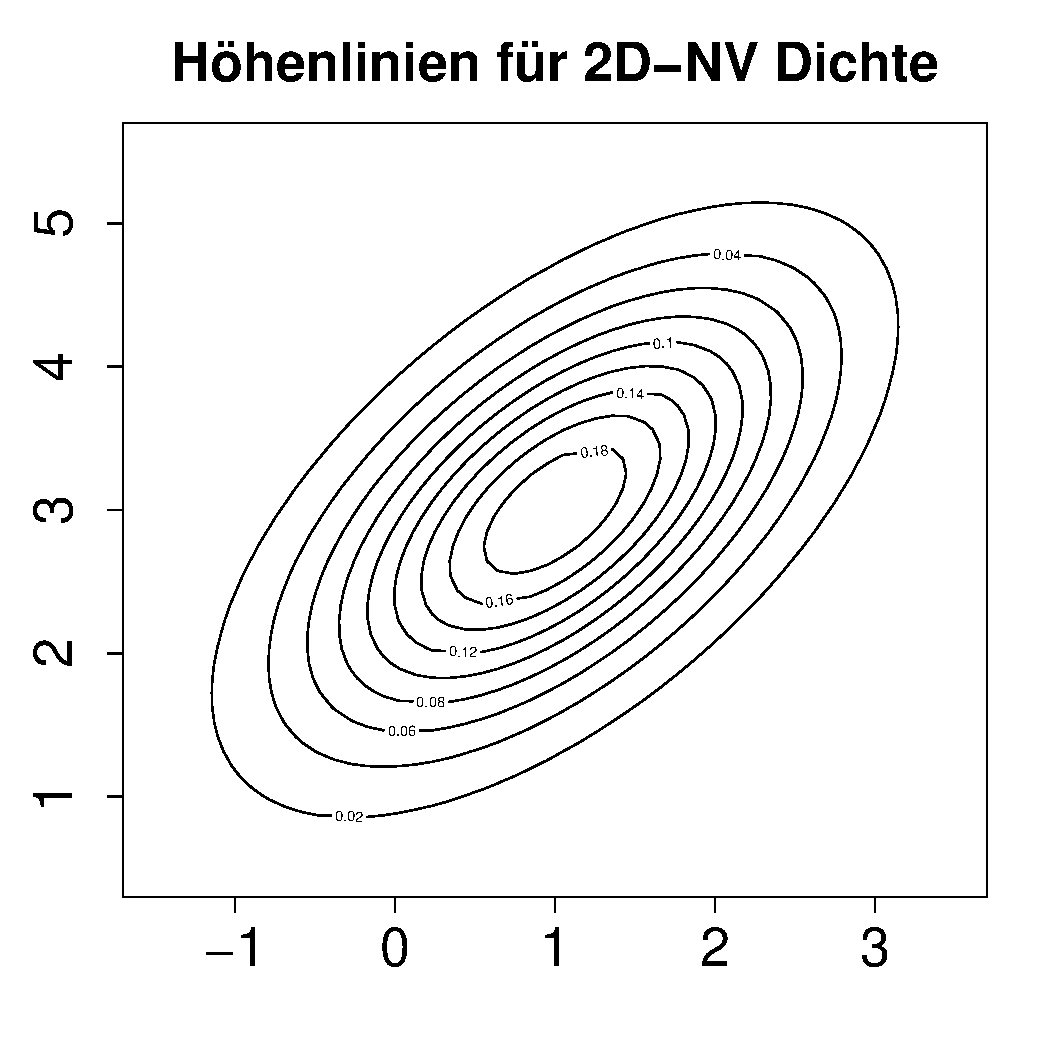
\includegraphics[width=6.25cm]{3dContour}
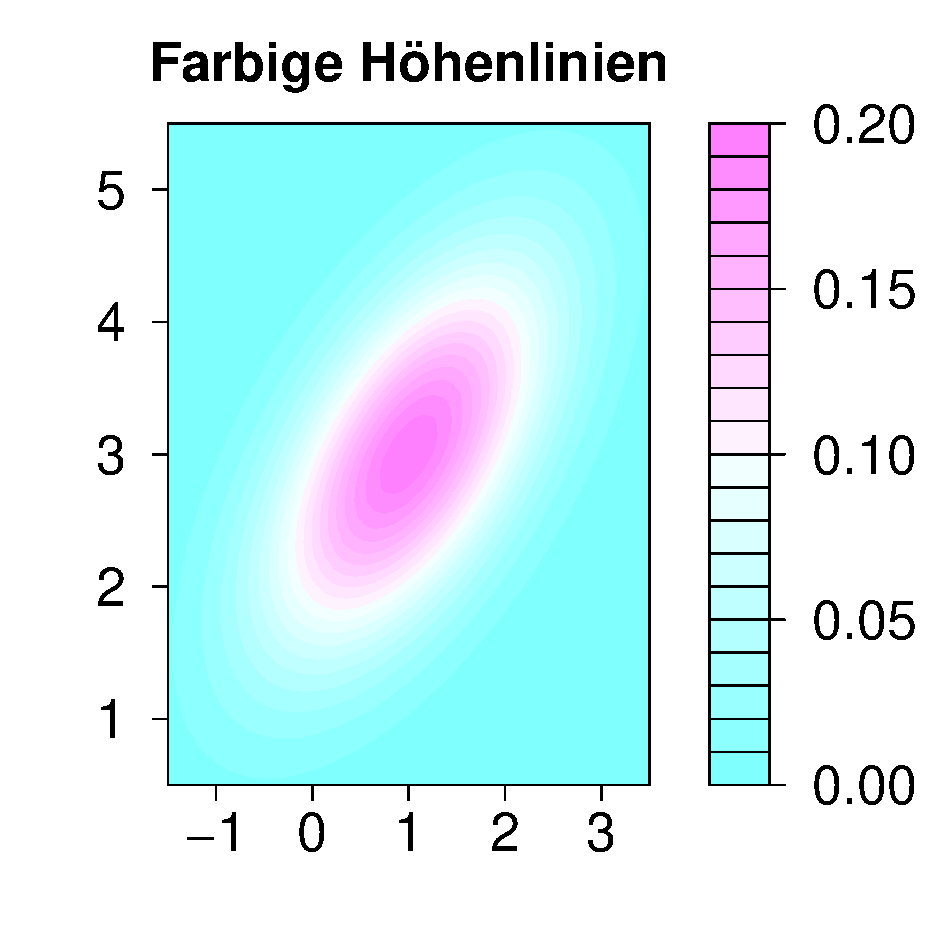
\includegraphics[width=6.25cm]{3dContourFilled}
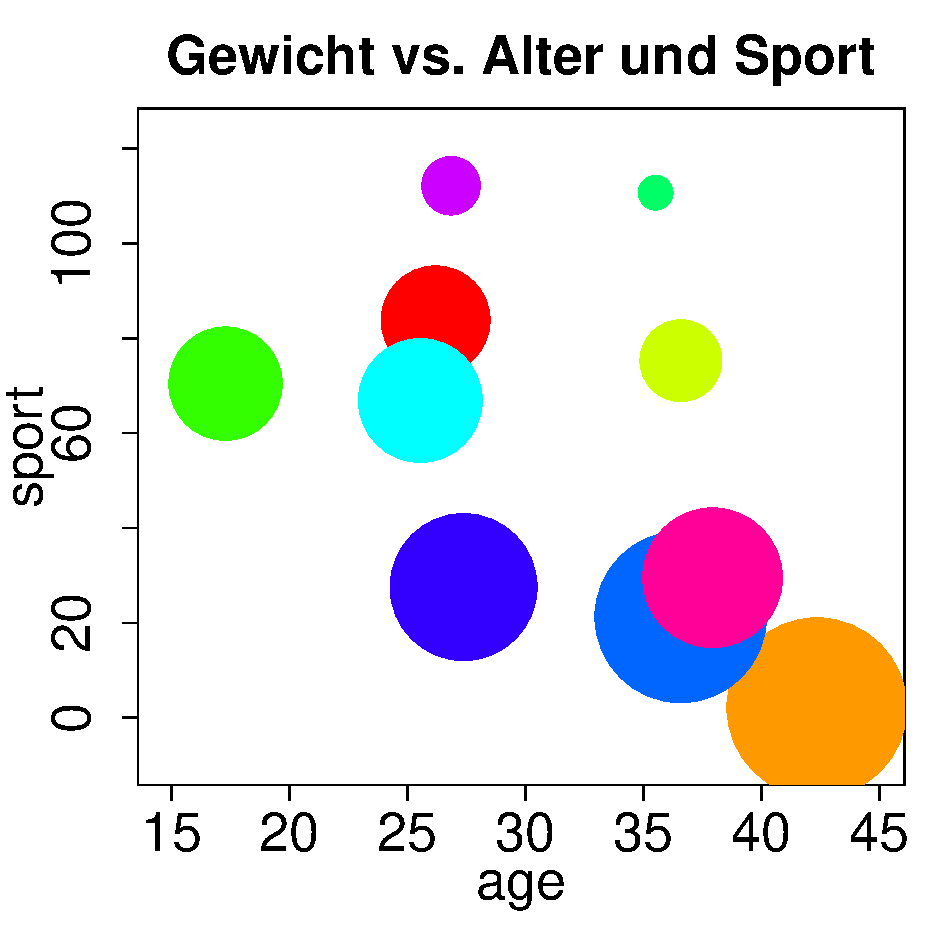
\includegraphics[width=6.25cm]{3dSymbols}
\vspace*{-1em}
\caption{Visualisierungsmöglichkeiten für dreidimensionale Daten: Höhenlinien und variable Datenpunktsymbole}
\label{fig:3dOne}
\end{figure}

%%%%%%%%%%%%%%%%%%%%%%%%%%%%%%%%%%%%%%%%%%%%%%%%%%%%%%%%%%%%%%%%%%
%%%%%%%%%%%%%%%%%%%%%%%%%%%%%%%%%%%%%%%%%%%%%%%%%%%%%%%%%%%%%%%%%%
\subsection{Dreidimensionale Gitter und Streudiagrammme}
\label{sec:3dGrid}
%%%%%%%%%%%%%%%%%%%%%%%%%%%%%%%%%%%%%%%%%%%%%%%%%%%%%%%%%%%%%%%%%%
%%%%%%%%%%%%%%%%%%%%%%%%%%%%%%%%%%%%%%%%%%%%%%%%%%%%%%%%%%%%%%%%%%

\index{Grafik!3D Gitter-Diagramm}
\lstinline!persp()!\index[func]{persp()@\lstinline{persp()}} erzeugt Diagramme mit Tiefeneindruck, in der die Datenpunkte zu einer Gitterfläche verbunden sind. Der Augpunkt, d.\,h.\ die Perspektive, aus der die simulierte dreidimensionale Szene gezeigt wird, ist frei wählbar (Abb.\ \ref{fig:3dTwo}).\footnote{Grafisch sehr aufwendig gerenderte Darstellungen dreidimensionaler Szenen erzeugt das Paket\index[pack]{rayshader@\lstinline{rayshader}} \lstinline!rayshader!\cite{MorganWall2019}. Beispiele zeigt \url{https://github.com/tylermorganwall/rayshader/}}
\begin{lstlisting}
persp(x=<<x-Koordinaten>>, y=<<y-Koordinaten>>, z=<<z-Koordinaten>>,
      theta=0, phi=15, r=sqrt(3))
\end{lstlisting}

Die Argumente \lstinline!x!, \lstinline!y! und \lstinline!z! haben dieselbe Bedeutung wie in Höhenlinien-Diagrammen. Die Argumente \lstinline!theta!, \lstinline!phi! und \lstinline!r! bestimmen die Blickrichtung auf das Diagramm in Form von Polarkoordinaten, die innerhalb einer gedachten Kugel mit dem Ursprung des Koordinatensystems im Zentrum definiert sind. Dabei bezeichnet \lstinline!theta! den Azimuth (Längengrad) und \lstinline!phi! die Höhe über dem Äquator (Breitengrad, Elevation). Die Entfernung zum Diagramm als Kugelradius kontrolliert \lstinline!r!. Die Funktion verfügt über weitere Argumente, u.\,a.\ zur Kontrolle der perspektivischen Verzerrung und zur räumlichen Kompression der $z$-Achse.
\begin{lstlisting}
> persp(X, Y, matZ, xlab="x", ylab="y", zlab="Dichte", theta=5,
+       phi=35, main="Dichte einer 2D Normalverteilung")
\end{lstlisting}

\index{Grafik!3D Streudiagramm}
\index[pack]{rgl@\lstinline{rgl}}
\index{Grafik!interaktive}
Mit Funktionen aus dem Paket \lstinline!rgl! \cite{Adler2011} erstellte Diagramme -- etwa\index[func]{plot3d()@\lstinline{plot3d()}} \lstinline!plot3d()!, \lstinline!hist3d()!\index[func]{hist3d()@\lstinline{hist3d()}} oder\index[func]{persp3d()@\lstinline{persp3d()}} \lstinline!persp3d()! als Pendants zu den konventionellen Funktionen \lstinline!plot()!, \lstinline!hist()! und \lstinline!persp()!, erlauben durch den Einsatz der Grafikbibliothek OpenGL eine interaktive Manipulation:\footnote{ %Auch\index{Grafik!interaktive} die Pakete\index[pack]{rggobi@\lstinline{rggobi}} \lstinline!rggobi! \cite{TempleLang2009} und \lstinline!playwith!\index[pack]{playwith@\lstinline{playwith}} \cite{Andrews2010} stellen Funktionen bereit, die Grafiken interaktiv in Echtzeit verändern, sie etwa an geänderte Ursprungsdaten anpassen.%
Sehr dynamisch ist derzeit die Entwicklung von Paketen, die interaktive Diagramme für Webseiten mit Hilfe von JavaScript-Bibliotheken implementieren. Dazu zählen\index[pack]{googleVis@\lstinline{googleVis}} \lstinline!googleVis! \cite{Gesmann2011} und \lstinline!plotly!\index[pack]{plotly@\lstinline{plotly}} \cite{Sievert2015,Sievert2020}.} Durch Anklicken der Diagrammfläche lässt sich die Perspektive auf das Diagramm beliebig ändern, indem die linke Maustaste gedrückt gehalten und die Maus bewegt wird (Abb.\ \ref{fig:3dTwo}).
\begin{lstlisting}
plot3d(x=<<x-Koordinaten>>, y=<<x-Koordinaten>>, z=<<x-Koordinaten>>)
\end{lstlisting}

Im Unterschied zu \lstinline!contour()! und \lstinline!persp()! müssen die $(x, y, z)$-Koordinaten der Punkte hier in Form dreier Vektoren gleicher Länge an die Argumente \lstinline!x!, \lstinline!y! und \lstinline!z! übergeben werden. Das \lstinline!rgl! Paket bringt eigene Funktionen zum Einfügen aller in Abschn.\ \ref{sec:graphAddElem} für zweidimensionale Diagramme beschriebenen Grafikelemente mit, vgl.\ \lstinline!help(package="rgl")!.
\begin{lstlisting}
> vecX <- rep(seq(-10, 10, length.out=10), times=10)
> vecY <- rep(seq(-10, 10, length.out=10),  each=10)
> vecZ <- vecX*vecY
> library(rgl)                                      # für plot3d()
> plot3d(vecX, vecY, vecZ, main="3D Scatterplot",
+        col="blue", type="h", aspect=TRUE)

> spheres3d(vecX, vecY, vecZ, col="red", radius=2)
> grid3d(c("x", "y+", "z"))
\end{lstlisting}

\begin{figure}[ht]
\centering
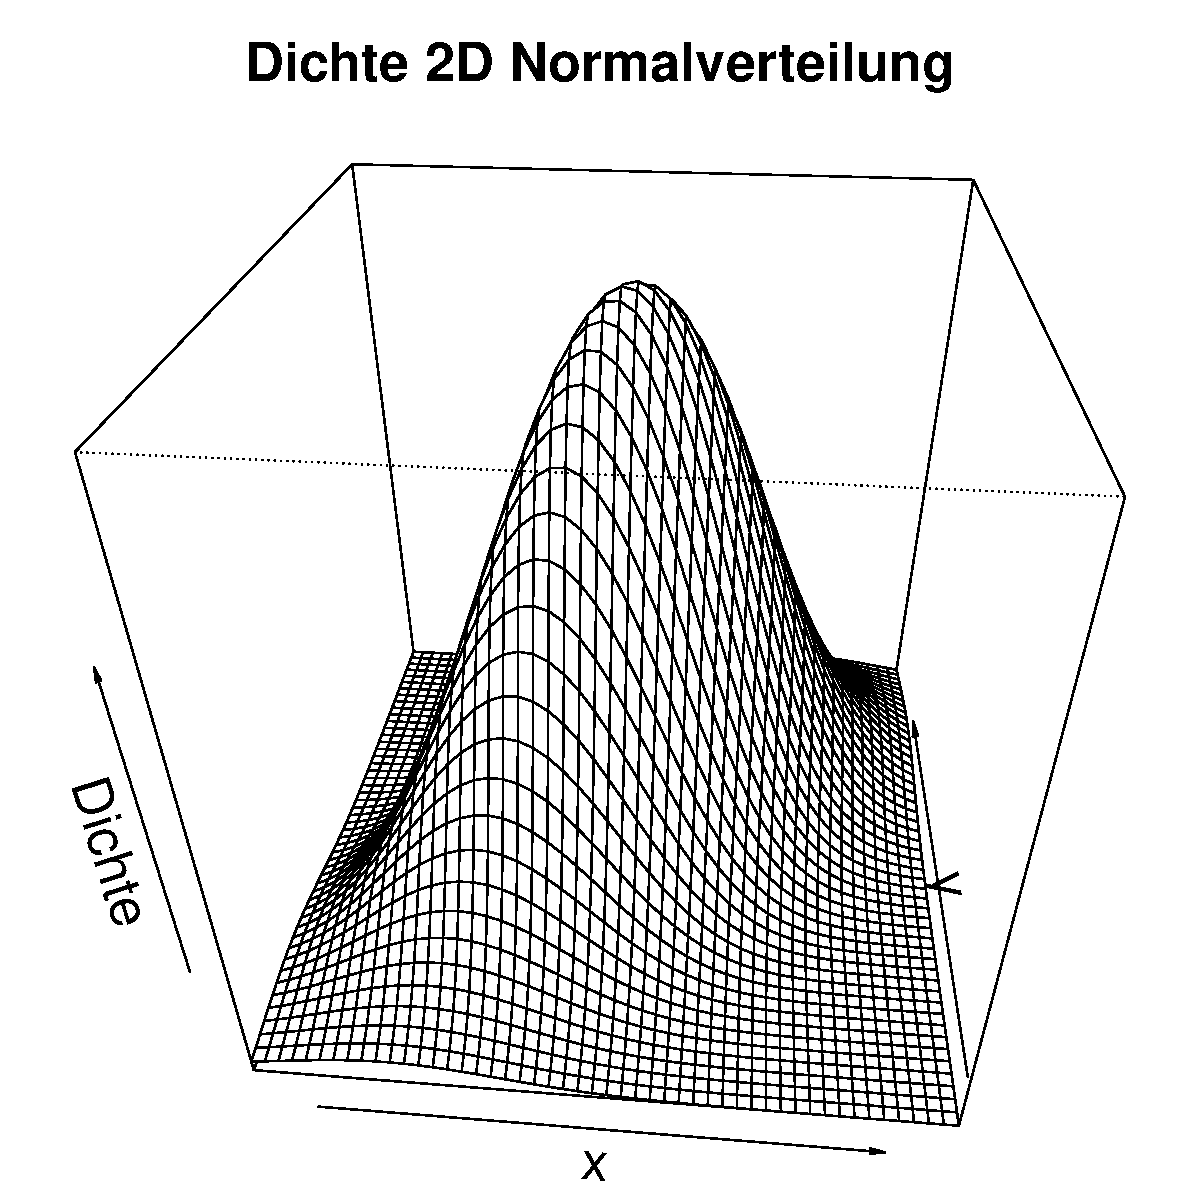
\includegraphics[width=5.7cm]{3dGridScatter1}
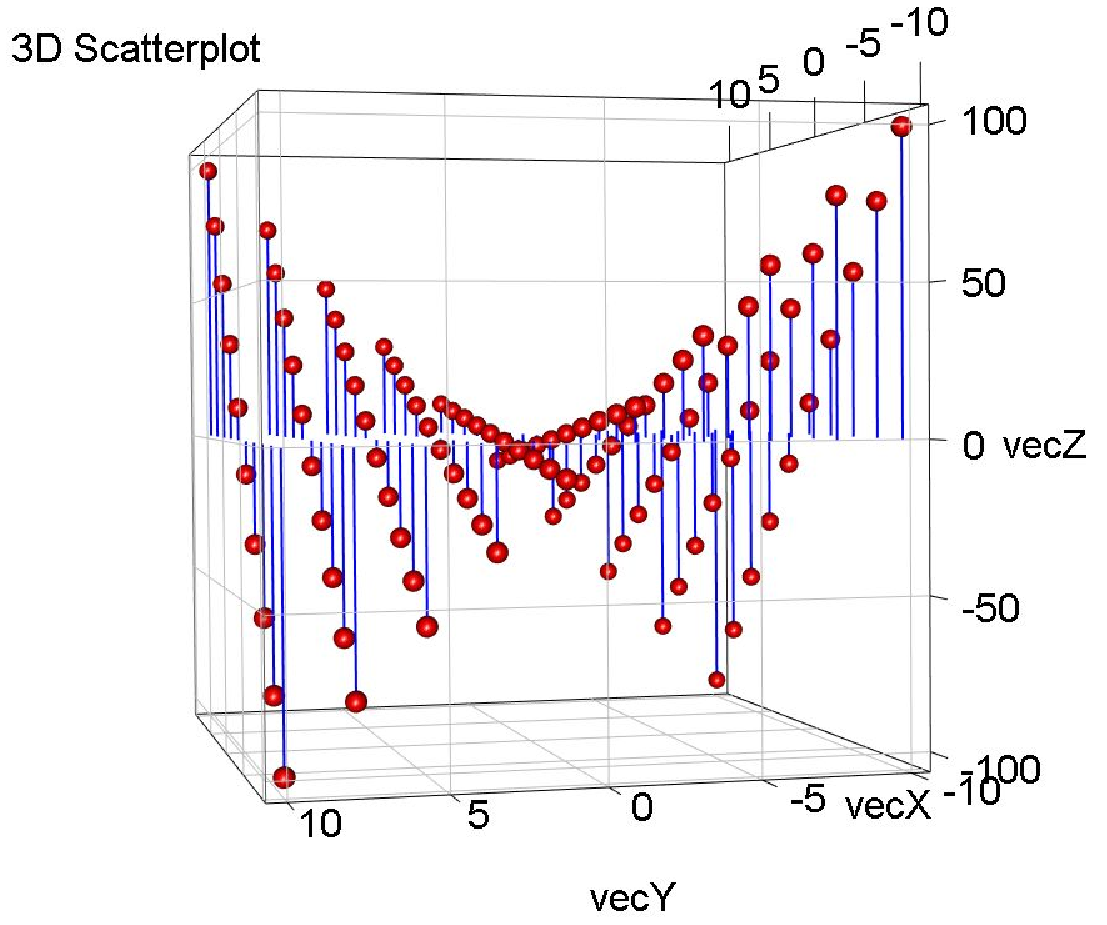
\includegraphics[width=6.7cm]{3dGridScatter2}
\vspace*{-0.5em}
\caption{Visualisierungsmöglichkeiten für dreidimensionale Daten: Gitter und interaktives Streudiagramm}
\label{fig:3dTwo}
\end{figure}

Das \lstinline!rgl! Paket enthält viele Zusatzfunktionen, mit denen der dreidimensionale Eindruck eines Diagramms über die Plazierung von Lichtquellen und die Manipulation von simulierten Oberflächenbeschaffenheiten gesteigert werden kann. Nach Laden des Pakets mit \lstinline!library(rgl)! erhält man durch\index[func]{demo()@\lstinline{demo()}} \lstinline!demo(rgl)! sowie insbesondere \lstinline!example(persp3d)! einen Überblick über die zahlreichen Gestaltungsmöglichkeiten.

%%%%%%%%%%%%%%%%%%%%%%%%%%%%%%%%%%%%%%%%%%%%%%%%%%%%%%%%%%%%%%%%%%%
%%%%%%%%%%%%%%%%%%%%%%%%%%%%%%%%%%%%%%%%%%%%%%%%%%%%%%%%%%%%%%%%%%%
%\subsection{Bedingte Diagramme für mehrere Gruppen mit \texttt{lattice}}
%\label{sec:lattice}
%%%%%%%%%%%%%%%%%%%%%%%%%%%%%%%%%%%%%%%%%%%%%%%%%%%%%%%%%%%%%%%%%%%
%%%%%%%%%%%%%%%%%%%%%%%%%%%%%%%%%%%%%%%%%%%%%%%%%%%%%%%%%%%%%%%%%%%
%
%\index[pack]{lattice@\lstinline{lattice}}
%Das Paket \lstinline!lattice! stellt viele Funktionen bereit, um Diagramme zu erzeugen, die Daten getrennt nach Gruppen simultan in mehreren Facetten darstellen (Abb.\ \ref{fig:coplotHist}, Abschn.\ \ref{sec:ggplot}, Fußnote \ref{ftn:ggplotLattice}). Diese Darstellungsart erlaubt es, alle hier bereits dargestellten Diagrammtypen zu verwenden, etwa Streudiagramme mit\index[func]{xyplot()@\lstinline{xyplot()}} \lstinline!xyplot()!, Säulendiagramme mit\index[func]{barchart()@\lstinline{barchart()}} \lstinline!barchart()!, dotcharts mit\index[func]{dotplot()@\lstinline{dotplot()}} \lstinline!dotplot()!, boxplots mit\index[func]{bwplot()@\lstinline{bwplot()}} \lstinline!bwplot()!, stripcharts mit\index[func]{stripplot()@\lstinline{stripplot()}} \lstinline!stripplot()! oder Histogramme mit\index[func]{histogram()@\lstinline{histogram()}} \lstinline!histogram()!. Der Aufruf all dieser Funktionen erfolgt immer in folgender Grundform:
%\begin{lstlisting}
%> xyplot(<<y-Koordinaten>> ~ <<x-Koordinaten>> | <<Faktor>>, data=<<Datensatz>>)
%\end{lstlisting}
%
%Als erstes Argument ist eine Modellformel anzugeben, die wie in \lstinline!plot()! zunächst die $(x, y)$-Koordinaten der darzustellenden Datenpunkte nennt. Als Besonderheit folgt dann hinter dem \lstinline!|! Zeichen ein Faktor, der die Gruppen definiert, für die separate Diagramme erstellt werden sollen. Die Unterteilung kann auch durch die Kombination mehrerer Faktoren definiert sein, die dann in der Form \lstinline!<<Faktor1>> * <<Faktor2>>! einzufügen sind. Stammen die in der Modellformel verwendeten Variablen aus einem Datensatz, ist dieser unter \lstinline!data! zu nennen. Weitere Details enthalten die zugehörigen Hilfe-Seiten sowie \citeA{Murrell2005} und \citeA{Sarkar2008}.
%\begin{lstlisting}
%> library(lattice)                                    # für histogram()
%> histogram(IQ ~ height | sex*group, data=myDf,
%+           main="Histogramme pro Gruppe")
%\end{lstlisting}
%
%\begin{figure}[ht]
%\centering
%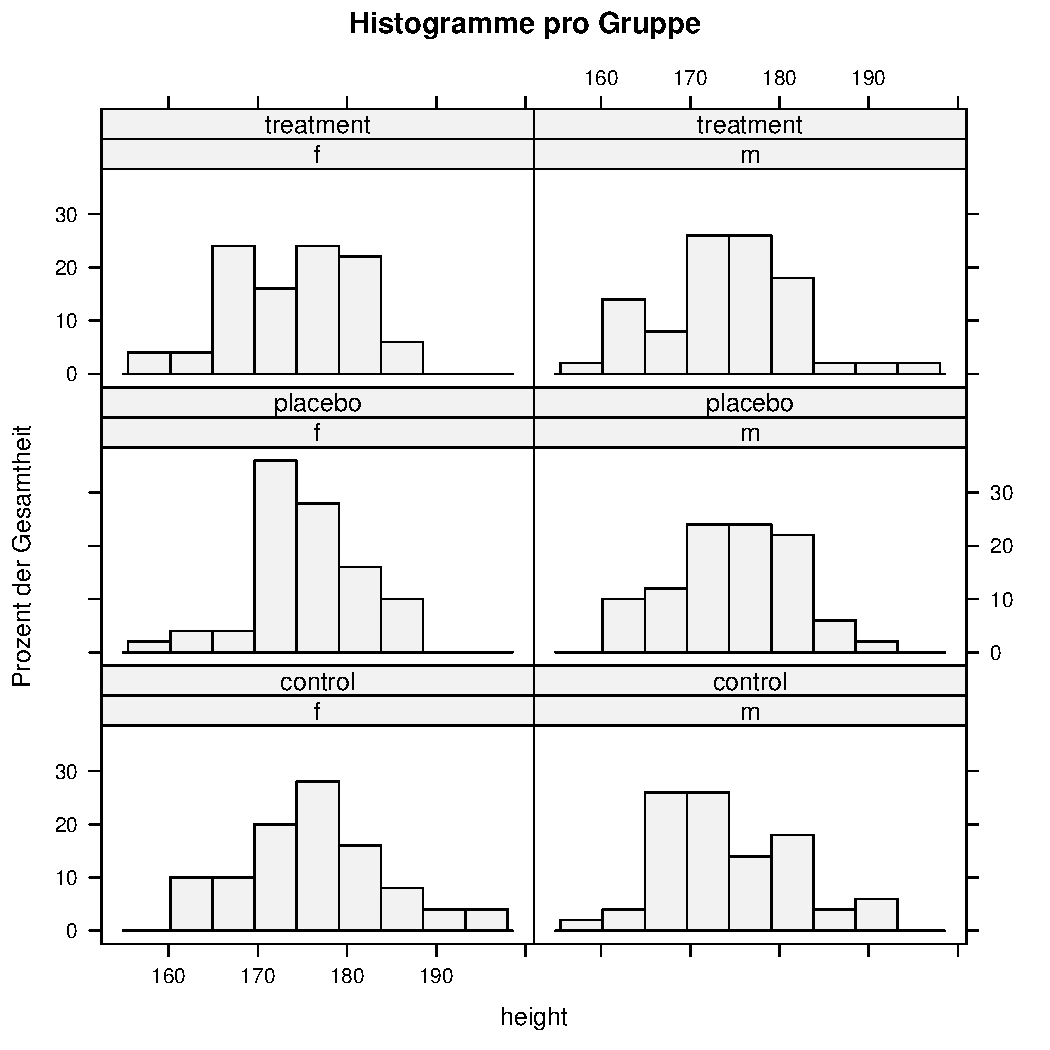
\includegraphics[width=7cm]{histogram}
%\vspace*{-1em}
%\caption{Darstellung multivariater Daten mit \lstinline!histogram()!}
%\label{fig:coplotHist}
%\end{figure}

%%%%%%%%%%%%%%%%%%%%%%%%%%%%%%%%%%%%%%%%%%%%%%%%%%%%%%%%%%%%%%%%%%
%%%%%%%%%%%%%%%%%%%%%%%%%%%%%%%%%%%%%%%%%%%%%%%%%%%%%%%%%%%%%%%%%%
\subsection{Matrix aus Streudiagrammen}
\label{sec:pairs}
%%%%%%%%%%%%%%%%%%%%%%%%%%%%%%%%%%%%%%%%%%%%%%%%%%%%%%%%%%%%%%%%%%
%%%%%%%%%%%%%%%%%%%%%%%%%%%%%%%%%%%%%%%%%%%%%%%%%%%%%%%%%%%%%%%%%%

\index{Grafik!Streudiagramm-Matrix}
Enthält ein Datensatz viele Variablen, können ihre paarweise gebildeten gemeinsamen Verteilungen in einer Matrix aus Streudiagrammen simultan veranschaulicht werden, wie sie\index[func]{pairs()@\lstinline{pairs()}} \lstinline!pairs()! erzeugt. Die Matrix enthält jeweils so viele Zeilen und Spalten, wie Variablen vorhanden sind, wobei sich in einer Zelle $(i, j)$ das Streudiagramm der gemeinsamen Verteilung der $i$-ten und $j$-ten Variable befindet. Auf der Hauptdiagonale (Zellen $(i, i)$) werden in der Voreinstellung die Variablennamen ausgegeben. An der Hauptdiagonale gespiegelte Zellen ($(i, j)$ und $(j, i)$) stellen dieselbe gemeinsame Verteilung mit vertauschten Achsen dar (Abb.\ \ref{fig:pairs}).
\begin{lstlisting}
pairs(x=<<Formel>>, data=<<Datensatz>>,
      panel=<<Zeichenfunktion>>,
      lower.panel=<<Zeichenfunktion>>,
      upper.panel=<<Zeichenfunktion>>,
      diag.panel=<<Zeichenfunktion>>)
\end{lstlisting}

Für \lstinline!x! ist die rechte Seite einer Modellformel \lstinline!~ <<Var1>> + <<Var2>> + ...! mit Variablen anzugeben, die aus einem Datensatz \lstinline!data! stammen, und deren paarweise gemeinsame Verteilungen dargestellt werden sollen. \lstinline!panel! erwartet den Namen einer Zeichenfunktion, deren Ergebnis in den Zellen außerhalb der Diagonale der erzeugten Grafik-Matrix abgebildet wird. Die Funktion muss als Argumente zwei Vektoren (Variablen aus \lstinline!data!) verarbeiten können und darf kein neues Diagramm öffnen, muss also eine Low-Level-Funktion sein. Voreinstellung ist \lstinline!points! für ein Streudiagramm. Sollen die Zellen oberhalb und unterhalb der Hauptdiagonale unterschiedliche Diagrammtypen zeigen, können für \lstinline!lower.panel! und \lstinline!upper.panel! separate Zeichenfunktionen angegeben werden, die denselben Bedingungen wie jene für \lstinline!panel! unterliegen. Durch Angabe einer Zeichenfunktion für \lstinline!diag.panel!, die als Argument die Daten der Variable $i$ erhält, lassen sich auch auf der Diagonale Diagramme einfügen (Voreinstellung ist \lstinline!NULL! für die Ausgabe der Variablennamen).

Im Beispiel seien Personen in zwei Gruppen aufgeteilt und an ihnen vier Variablen erhoben worden. Die Streudiagramme sollen die Gruppenzugehörigkeit über Art und Farbe der Datenpunktsymbole kenntlich machen (Abschn.\ \ref{sec:distr2var}).
\begin{lstlisting}
> N  <- 20                                       # Gesamt-N
> P  <- 2                                        # Anzahl Gruppen
> IV <- factor(rep(c("CG", "T"), each=N/P))      # Gruppenzugehörigkeit

# abhängige Variablen
> age    <- sample(18:35, N, replace=TRUE)
> IQ     <- round(rnorm(N, rep(c(100, 115), each=N/P), 15))
> rating <- round(0.4*IQ - 30 + rnorm(N, 0, 10), 1)
> score  <- round(-0.3*IQ + 0.7*age + rnorm(N, 0, 8), 1)
> mvDf   <- data.frame(IV, age, IQ, rating, score)          # Datensatz

# Matrix aus Streudiagrammen darstellen
> pairs(~ age + IQ + rating + score, main="Streudiagramm-Matrix",
+       data=mvDf,
+       pch=c(4, 16)[unclass(IV)], col=c("red", "blue")[unclass(IV)])
\end{lstlisting}

Da sich nur Low-Level Zeichenfunktionen für die \lstinline!panel! Argumente eignen, ist häufig der Umweg über selbst erstellte Funktionen notwendig, um bestimmte Grafiken in der Matrix darzustellen (Abschn.\ \ref{sec:function}): Für High-Level-Funktionen muss dafür zunächst \lstinline!par(new=TRUE)! aufgerufen werden, damit sie selbst kein neues device öffnen (Abschn.\ \ref{sec:parMfRow}).

Hier soll dies zunächst für in der Hauptdiagonale darzustellende Histogramme geschehen. Zusätzlich sollen die für beide Gruppen getrennten Streuungsellipsen der gemeinsamen Verteilung in den Zellen oberhalb der Hauptdiagonale gezeigt werden (Abb.\ \ref{fig:distr2var}, Abschn.\ \ref{sec:distr2var}).
\begin{lstlisting}
# Funktion, um Histogramm darzustellen, ohne neue Grafik zu öffnen
> myHist <- function(x, ...) { par(new=TRUE); hist(x, ..., main="") }

# Funktion, um Streuungsellipsen getrennt für beide Gruppen zu zeichnen
> library(car)                              # für ellipse()
> myEll <- function(x, y, ...) { # ... für weitere Argumente aus pairs()
+     # trenne Beobachtungen in Variablen x und y nach Gruppen und
+     # verbinde Variablen getrennt nach Gruppen zu einer Datenmatrix
+     splLL <- split(data.frame(x, y), mvDf$IV)
+     matCG <- data.matrix(splLL$CG)        # Daten Gruppe 1
+     matT  <- data.matrix(splLL$T)         # Daten Gruppe 2
+     ctrCG <- colMeans(matCG)              # Zentroid Gruppe 1
+     ctrT  <- colMeans(matT)               # Zentroid Gruppe 2
+
+     # Ellipsen einzeichnen
+     ellipse(ctrCG, shape=cov(matCG), col="red",  radius=1)
+     ellipse(ctrT,  shape=cov(matT),  col="blue", radius=1)
}

> pairs(~ age + IQ + rating + score, diag.panel=myHist,
+       upper.panel=myEll, main="Streudiagramm-Matrix", pch=16,
+       col=c("red", "blue")[unclass(IV)])
\end{lstlisting}

\begin{figure}[ht]
\centering
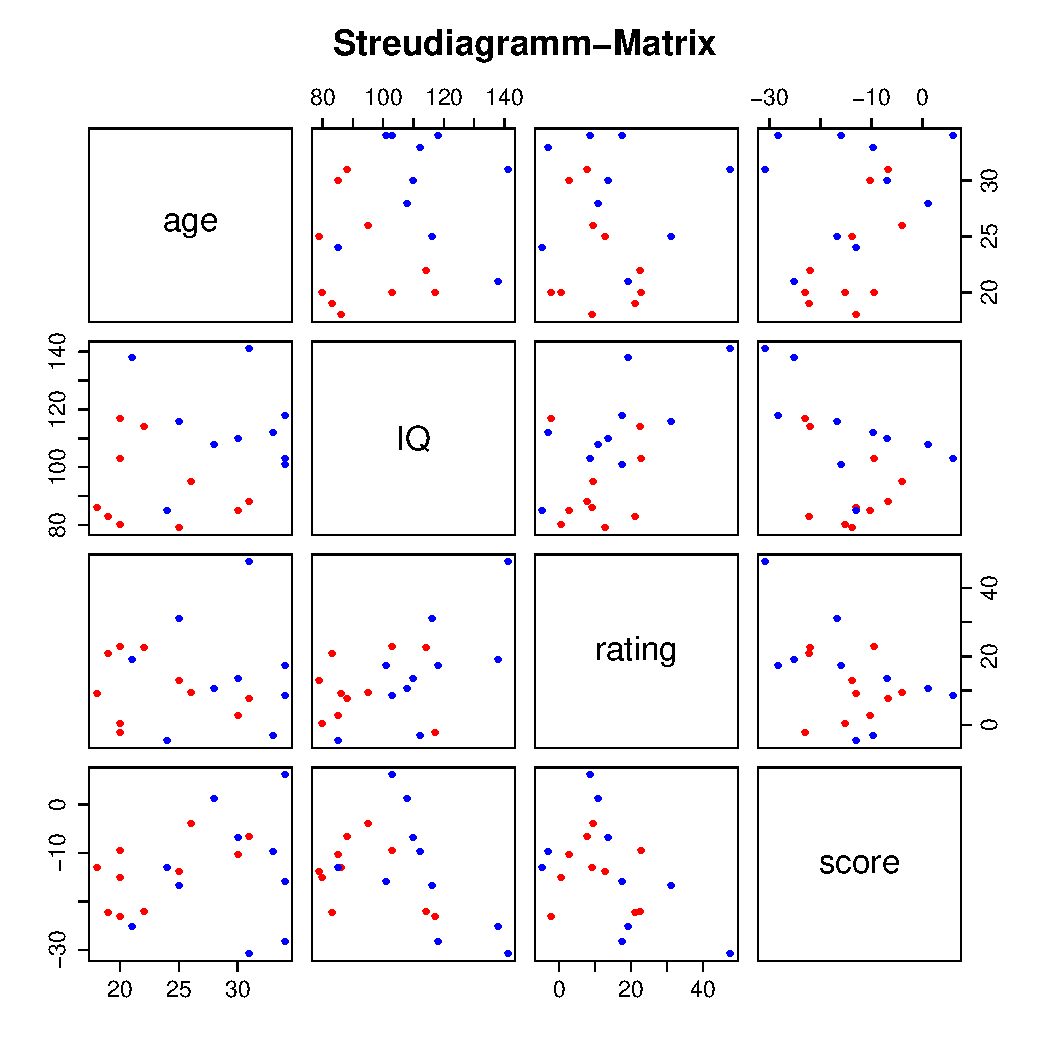
\includegraphics[width=6.25cm]{pairs1}
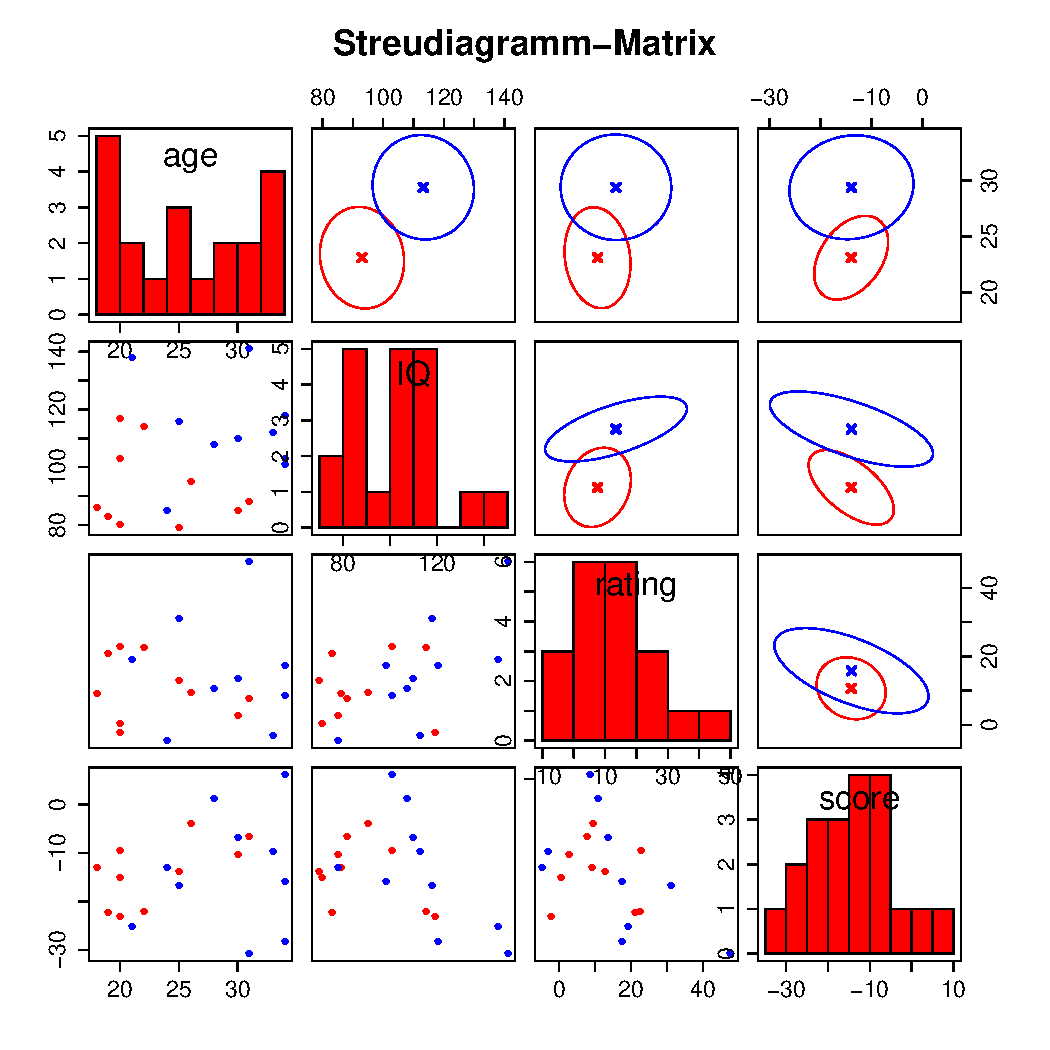
\includegraphics[width=6.25cm]{pairs2}
\vspace*{-1em}
\caption{Matrizen von paarweisen Streudiagrammen mehrerer Variablen mit \lstinline!pairs()!}
\label{fig:pairs}
\end{figure}

%%%%%%%%%%%%%%%%%%%%%%%%%%%%%%%%%%%%%%%%%%%%%%%%%%%%%%%%%%%%%%%%%%
%%%%%%%%%%%%%%%%%%%%%%%%%%%%%%%%%%%%%%%%%%%%%%%%%%%%%%%%%%%%%%%%%%
\subsection{Heatmap}
\label{sec:heatmap}
%%%%%%%%%%%%%%%%%%%%%%%%%%%%%%%%%%%%%%%%%%%%%%%%%%%%%%%%%%%%%%%%%%
%%%%%%%%%%%%%%%%%%%%%%%%%%%%%%%%%%%%%%%%%%%%%%%%%%%%%%%%%%%%%%%%%%

\index{Grafik!heatmap}
Eine \emph{heatmap} ist eine Falschfarben-Darstellung der Werte einer Matrix, wobei für jede Zelle eine Farbe entsprechend der Größe des Zellenwertes gewählt wird. Mit\index[func]{heatmap()@\lstinline{heatmap()}} \lstinline!heatmap()! können auf diese Weise etwa die Einträge der Korrelationsmatrix vieler Variablen so visualisiert werden, dass unmittelbar ersichtlich ist, welche Variablen einen starken linearen Zusammenhang aufweisen.\footnote{Ästhetisch ansprechendere heatmaps mit sehr viel mehr Gestaltungsmöglichkeiten bietet das Paket \index[pack]{pheatmap@\lstinline{pheatmap}} \lstinline!pheatmap! \cite{Kolde2015}.}
\begin{lstlisting}
heatmap(<<Matrix>>, symm, revC, Rowv, Colv, recV, col,
        RowSideColors, ColSideColors)
\end{lstlisting}

Das erste Argument erwartet eine numerische Matrix. Handelt es sich um eine symmetrische Matrix (z.\,B.\ eine Korrelationsmatrix), kann dies mit \lstinline!symm=TRUE! angezeigt werden. In diesem Fall sorgt \lstinline!revC=TRUE! dafür, dass die Reihenfolge von Zeilen und Spalten übereinstimmt. \lstinline!Rowv! und \lstinline!Colv! kontrollieren, ob an den Grafikrändern ein \emph{Dendrogramm} angezeigt werden soll, das die mit einer Clusteranalyse ermittelten hierarchischen Zusammenhänge von Variablen darstellt. Setzt man diese Argumente auf \lstinline!NA!, wird kein Dendrogramm angezeigt. Die zu verwendenden Farben können an \lstinline!col! übergeben werden, wobei soviele Farben wie Zellen vorhanden sein müssen. Um die Reihenfolge der Farben in einer Legende an den Seiten des Diagramms darzustellen, können sie an \lstinline!RowSideColors! (soviele Farben wie Zeilen) oder \lstinline!ColSideColors! (soviele Farben wie Spalten) übergeben werden.

Die Ausgabe entspricht der Struktur der übergebenen Matrix, wobei jede Zelle durch eine Farbe dargestellt wird (Abb.\ \ref{fig:heatmap}). Farben werden Werten so zugeordnet, dass die erste Farbe in \lstinline!col! zum kleinsten Wert gehört und die letzte Farbe zum größten Wert in der Matrix.
\begin{lstlisting}
> corMat <- cor(data.matrix(mvDf))          # Korrelationsmatrix
> round(corMat, digits=3)
          IV   age     IQ rating  score
IV     1.000 0.578  0.570  0.209  0.003
age    0.578 1.000  0.210  0.041  0.254
IQ     0.570 0.210  1.000  0.546 -0.435
rating 0.209 0.041  0.546  1.000 -0.458
score  0.003 0.254 -0.435 -0.458  1.000

> cmCol  <- rev(heat.colors(nrow(corMat))) # Basisfarben
> cmRamp <- colorRampPalette(cmCol)        # Funktion für Mischfarben
> cols   <- cmRamp(length(corMat))         # Mischfarben
> heatmap(corMat, symm=TRUE, revC=TRUE, Rowv=NA, Colv=NA, col=cols,
+         RowSideColors=cmCol, main="Heatmap einer Korrelationsmatrix")
\end{lstlisting}

\begin{figure}[ht]
\centering
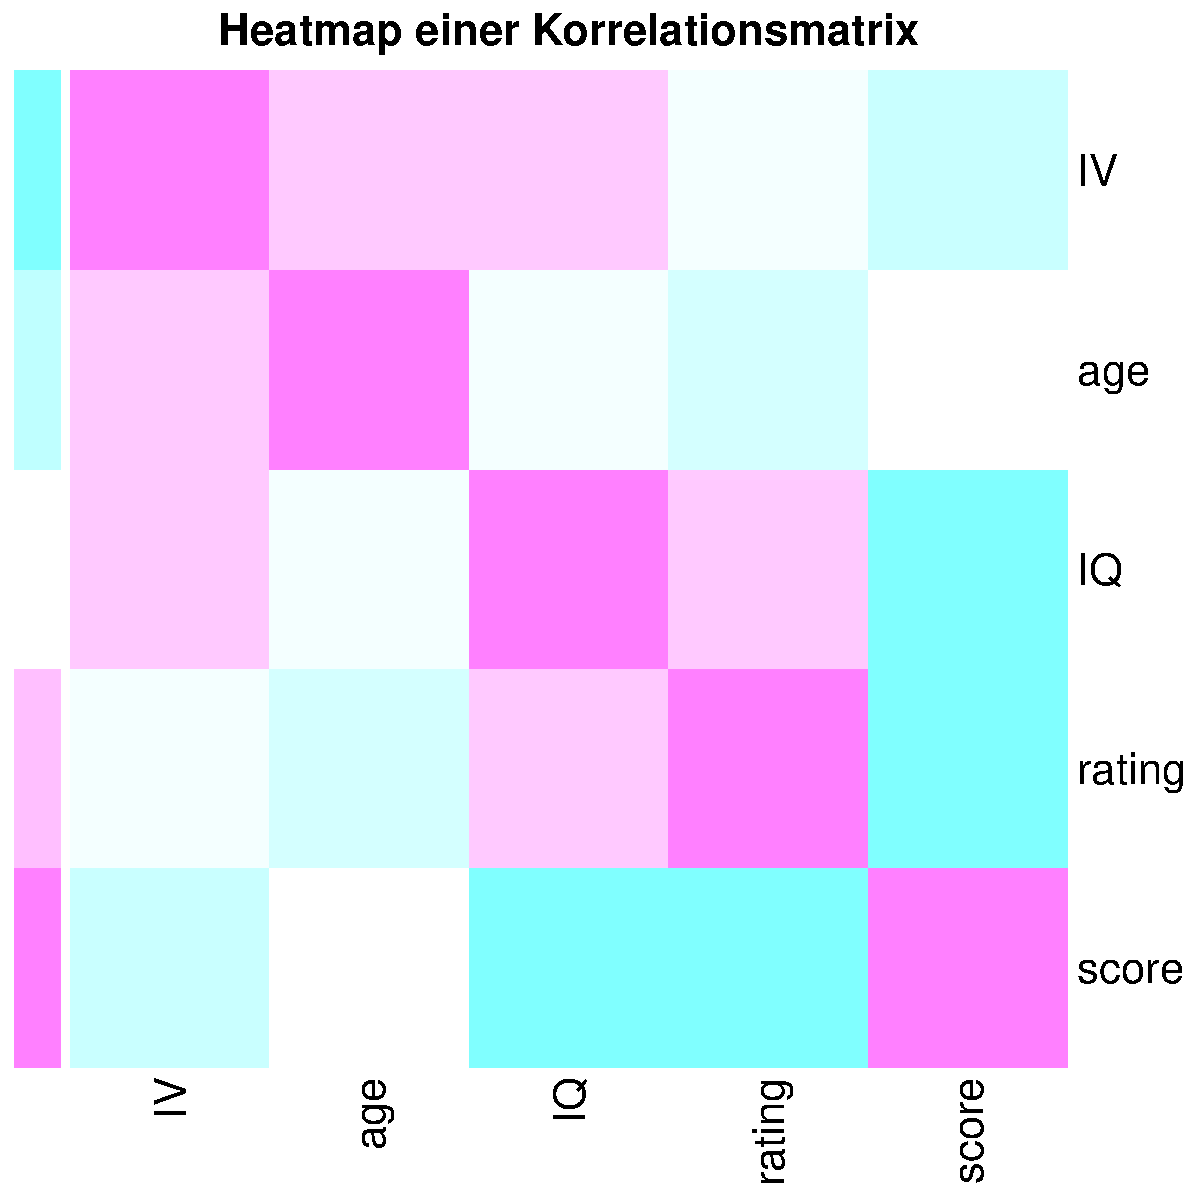
\includegraphics[width=8cm]{heatmap}
\vspace*{-1em}
\caption{Heatmap einer Korrelationsmatrix}
\label{fig:heatmap}
\end{figure}

\lstinline!heatmap()! verfügt über viele weitere Darstellungsmöglichkeiten, die insbesondere im Rahmen einer Clusteranalyse sinnvoll sind und in \lstinline!?heatmap! erläutert werden.

%%%%%%%%%%%%%%%%%%%%%%%%%%%%%%%%%%%%%%%%%%%%%%%%%%%%%%%%%%%%%%%%%%
%%%%%%%%%%%%%%%%%%%%%%%%%%%%%%%%%%%%%%%%%%%%%%%%%%%%%%%%%%%%%%%%%%
\section{Mehrere Diagramme in einem Grafik-Device darstellen}
\label{sec:diagSplit}
%%%%%%%%%%%%%%%%%%%%%%%%%%%%%%%%%%%%%%%%%%%%%%%%%%%%%%%%%%%%%%%%%%
%%%%%%%%%%%%%%%%%%%%%%%%%%%%%%%%%%%%%%%%%%%%%%%%%%%%%%%%%%%%%%%%%%

\index{Grafik!device!unterteilen}
\index{Grafik!mehrere Grafiken in einem device}
Die in Abschn.\ \ref{sec:pairs} vorgestellten Funktionen verdeutlichen, dass auch mehr als ein Diagramm in ein device gezeichnet werden kann. Sollen nicht nur Diagramme gleichen Typs, sondern auch unterschiedliche Grafiken in einem device dargestellt werden, lässt sich dessen Fläche manuell in mehrere rechteckige Bereiche aufteilen. Diese können dann mit jeweils einem Diagramm gefüllt werden. Auf diese Weise simultan dargestellte Diagramme erleichtern den Vergleich von Ergebnissen in verschiedenen Teilstichproben, lassen sich aber auch nutzen, um dieselben Daten parallel auf verschiedene Arten zu visualisieren.

%%%%%%%%%%%%%%%%%%%%%%%%%%%%%%%%%%%%%%%%%%%%%%%%%%%%%%%%%%%%%%%%%%
%%%%%%%%%%%%%%%%%%%%%%%%%%%%%%%%%%%%%%%%%%%%%%%%%%%%%%%%%%%%%%%%%%
\subsection{\texttt{layout()}}
%%%%%%%%%%%%%%%%%%%%%%%%%%%%%%%%%%%%%%%%%%%%%%%%%%%%%%%%%%%%%%%%%%
%%%%%%%%%%%%%%%%%%%%%%%%%%%%%%%%%%%%%%%%%%%%%%%%%%%%%%%%%%%%%%%%%%

\begin{figure}[ht]
\centering
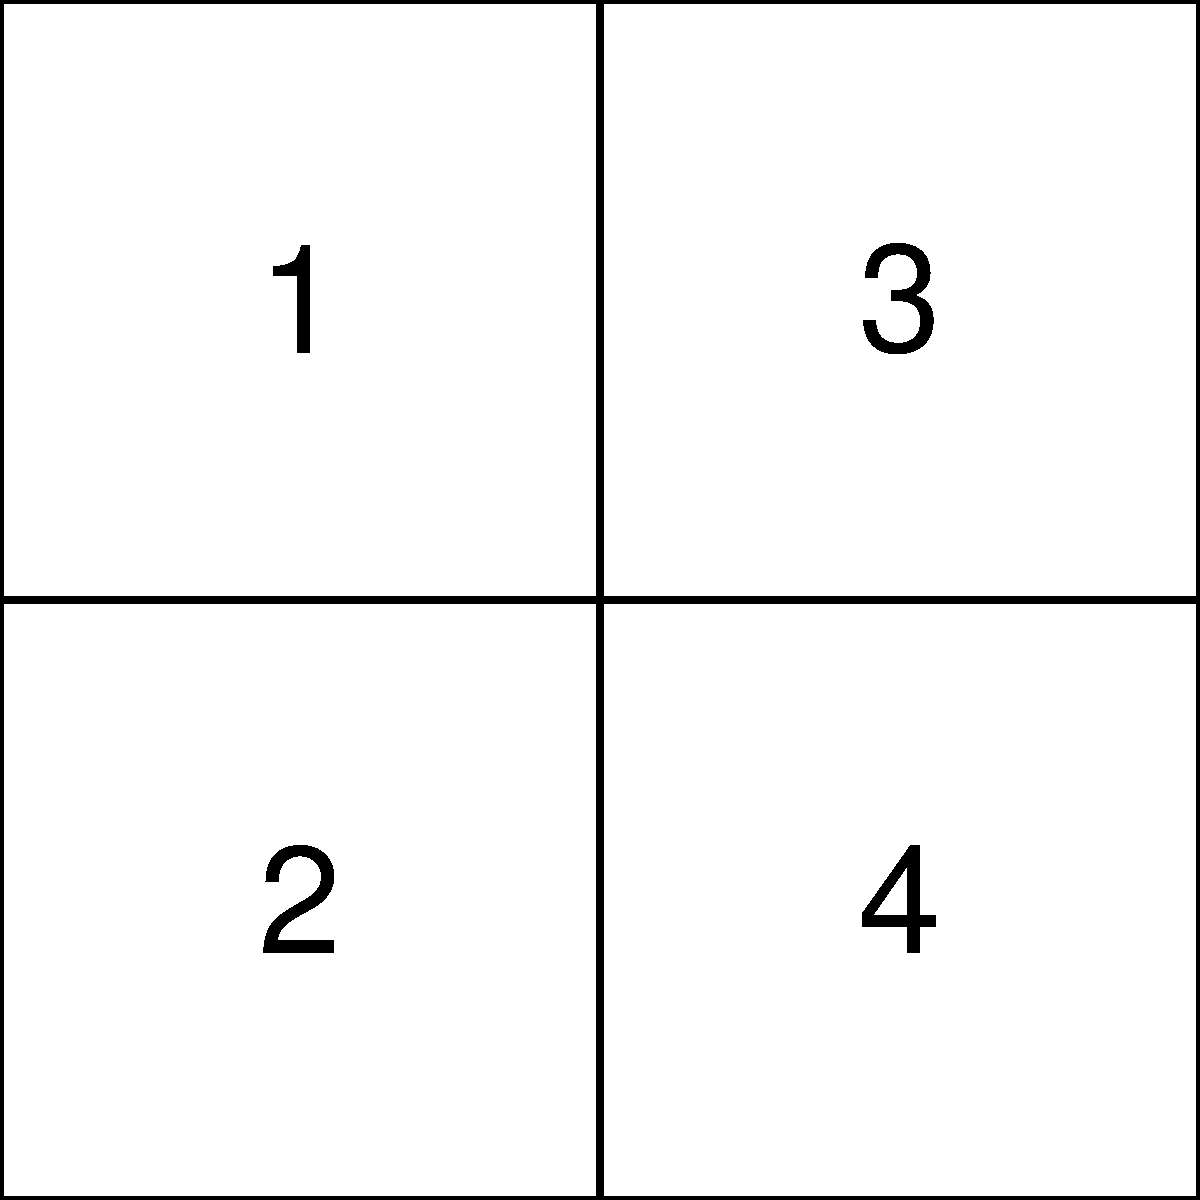
\includegraphics[width=4cm]{layoutShowA}
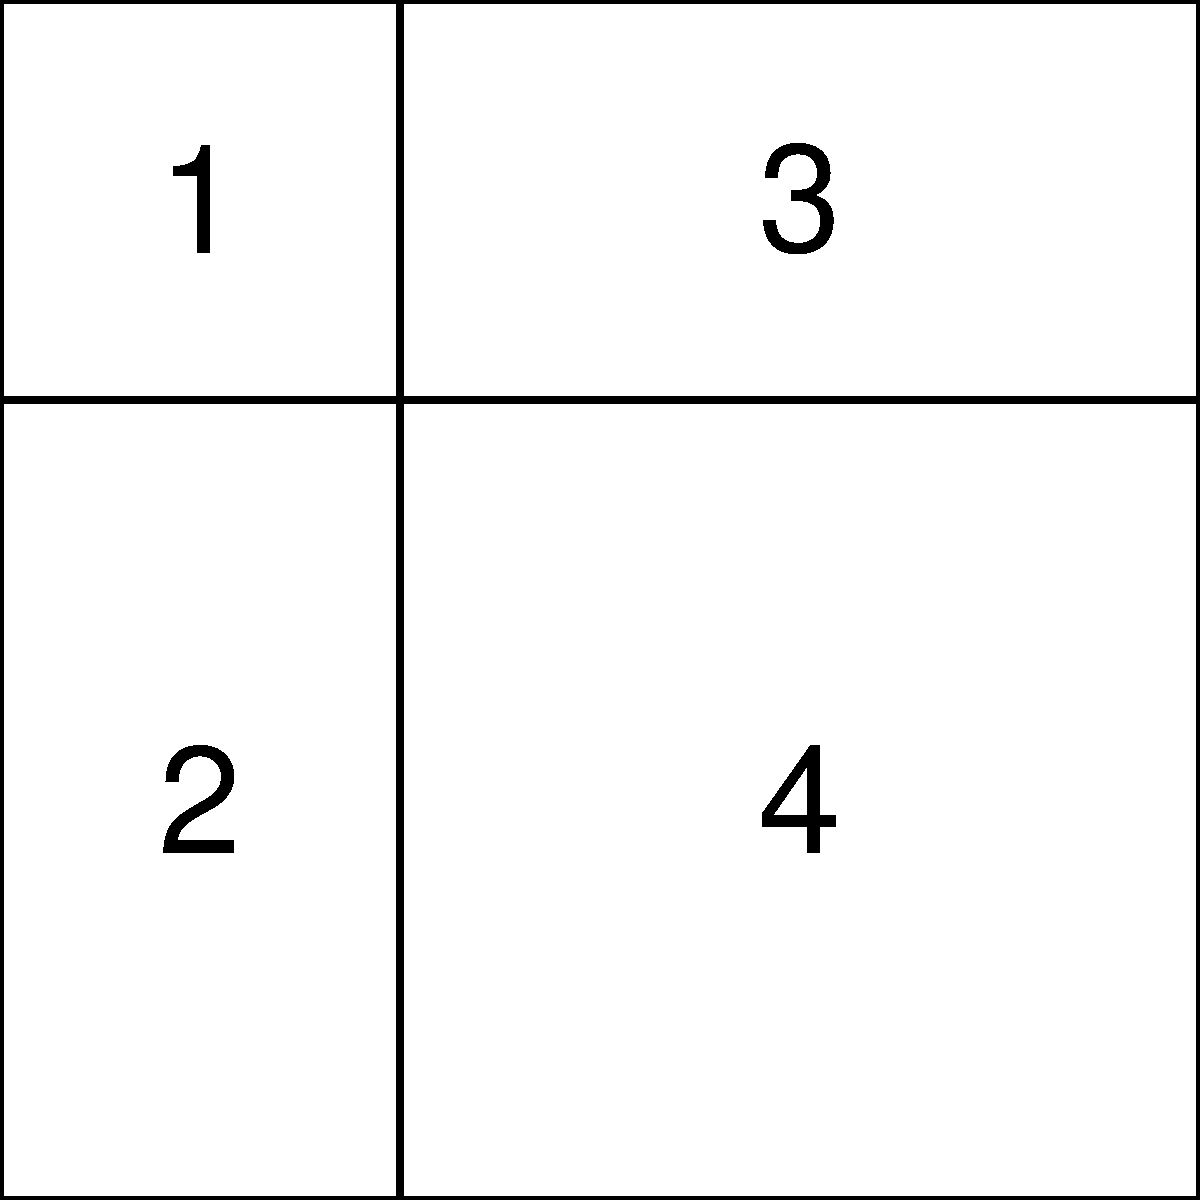
\includegraphics[width=4cm]{layoutShowB}
\vspace*{-0.5em}
\caption{Mit \lstinline!layout()! eingeteilte Regionen eines device
\label{fig:layoutShow}}
\end{figure}

Um $n$ Diagramme in einem device darzustellen, kann dessen Fläche mit\index[func]{layout()@\lstinline{layout()}} \lstinline!layout()! unter Zuhilfenahme einer Matrix \lstinline!mat! aufgeteilt werden, die aus den Zahlen $0, 1, \ldots, n$ gebildet ist. Die Ergebnisse der sich an \lstinline!layout()! anschließenden $n$ High-Level-Funktionen zum Erstellen von Diagrammen werden automatisch den durch \lstinline!mat! definierten Regionen zugewiesen, statt jeweils die gesamte Fläche des aktiven device zu überschreiben (Abb.\ \ref{fig:layoutShow}, \ref{fig:layout}).
\begin{lstlisting}
layout(mat=<<Matrix>>, widths=<<Vektor>>, heights=<<Vektor>>)
\end{lstlisting}

\lstinline!mat! bestimmt die Einteilung der Device-Region in Planquadrate, die durch die Zellen von \lstinline!mat! symbolisiert werden. Enthält eine Zelle von \lstinline!mat! dabei die $0$, wird die zugehörige Region beim Befüllen mit Grafiken übersprungen und bleibt leer. Dann ist die Anzahl $n$ der dargestellten Diagramme kleiner als die Zahl der Zellen von \lstinline!mat!, also der ursprünglichen Planquadrate. Über das Argument \lstinline!widths! ist die Breite der Spalten und über \lstinline!heights! die Höhe der Zeilen veränderbar -- in der Voreinstellung erfolgt die Aufteilung gleichmäßig (Abb.\ \ref{fig:layoutComb}). Breite und Höhe können zum einen als relative Größe in Form eines Vektors von ganzzahligen Gewichten ausgedrückt werden, die dann an der Summe aller Gewichte relativiert werden. Zum anderen können die Maße auch als absolute Werte mit\index[func]{lcm()@\lstinline{lcm()}} \lstinline!lcm(<<Zahl>>)! in der Einheit cm eingegeben werden. Um die $n$ Planquadrate durch Umrandung sichtbar zu machen, ist\index[func]{layout.show()@\lstinline{layout.show()}} \lstinline!layout.show(n)! zu verwenden.
\begin{lstlisting}
> (mat1 <- matrix(1:4, 2, 2))   # 4 Regionen derselben Größe definieren
    [,1]  [,2]
[1,]   1     3
[2,]   2     4

> layout(mat1)                                   # Device-Fläche teilen
> layout.show(4)                                 # Regionen anzeigen

# dieselben Regionen mit unterschiedlicher Größe
> layout(mat1, widths=c(1, 2), heights=c(1, 2))  # Aufteilung 1/3, 2/3
> layout.show(4)                                 # Regionen anzeigen

# vier Diagramme einfügen
> barplot(table(round(rnorm(100))), horiz=TRUE, main="Barplot")
> boxplot(rt(100, 5), main="Boxplot")
> stripchart(sample(1:20, 40, replace=TRUE), method="stack",
+            main="Stripchart")

> pie(table(sample(1:6, 20, replace=TRUE)), main="Kreisdiagramm")
\end{lstlisting}

\begin{figure}[ht]
\centering
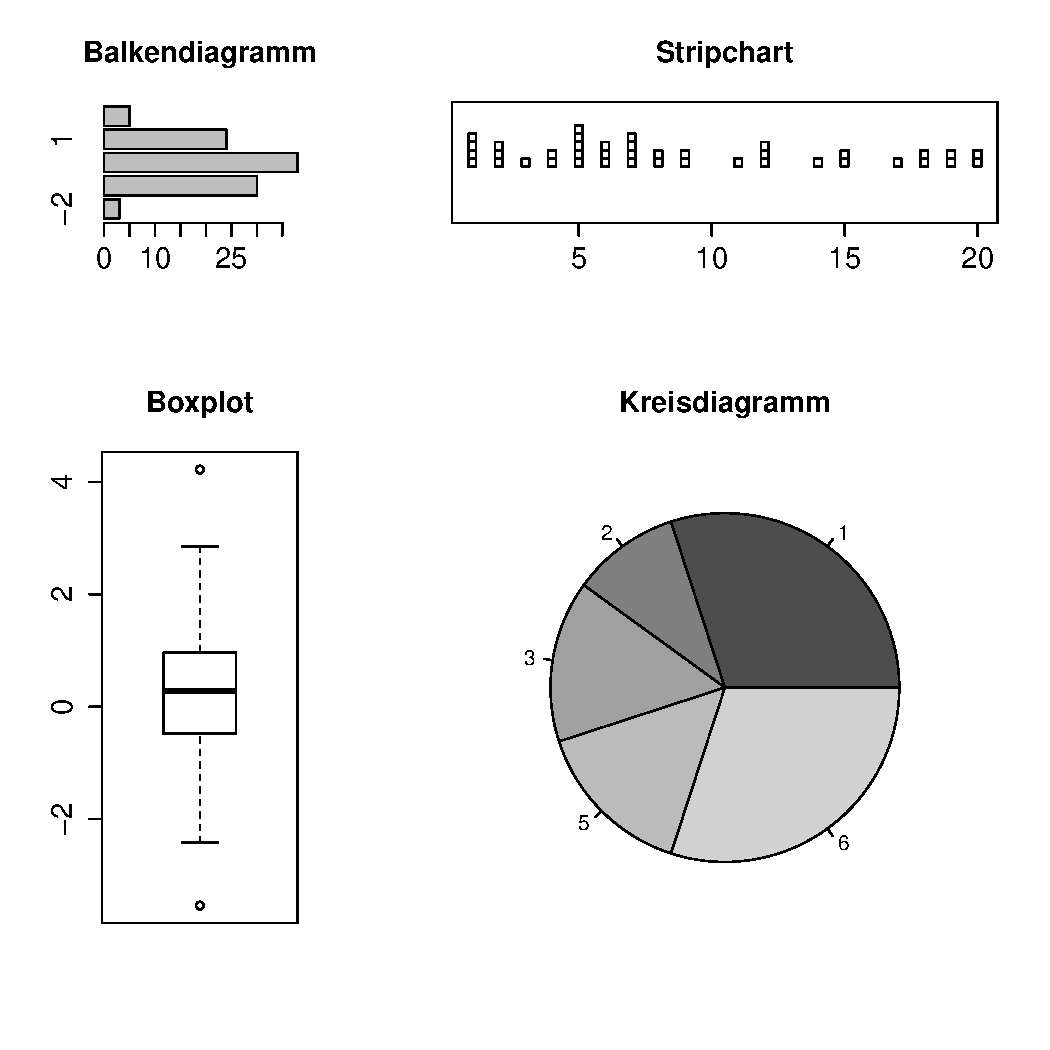
\includegraphics[width=8cm]{layout}
\vspace*{-1em}
\caption{Verschiedene Diagramme in einem Diagrammfenster mittels \lstinline!layout()!}
\label{fig:layout}
\end{figure}

Benachbarte Planquadrate der Device-Fläche lassen sich zusammenfassen, indem den zugehörigen Matrixelementen dieselbe Zahl zugeordnet wird (Abb.\ \ref{fig:layoutComb}). Auch hier ist die Anzahl $n$ der dargestellten Diagramme kleiner als die Zahl der Zellen von \lstinline!mat!.
\begin{lstlisting}
# Zellen der ersten Zeile zusammenfassen, Region links unten leer
> (mat2 <- matrix(c(1, 0, 1, 2), 2, 2))
    [,1]  [,2]
[1,]   1     1
[2,]   0     2

> layout(mat2)
> stripchart(sample(1:20, 40, replace=TRUE), method="stack",
+            main="Stripchart")

> barplot(table(round(rnorm(100))), main="Säulendiagramm")
\end{lstlisting}

\begin{figure}[ht]
\centering
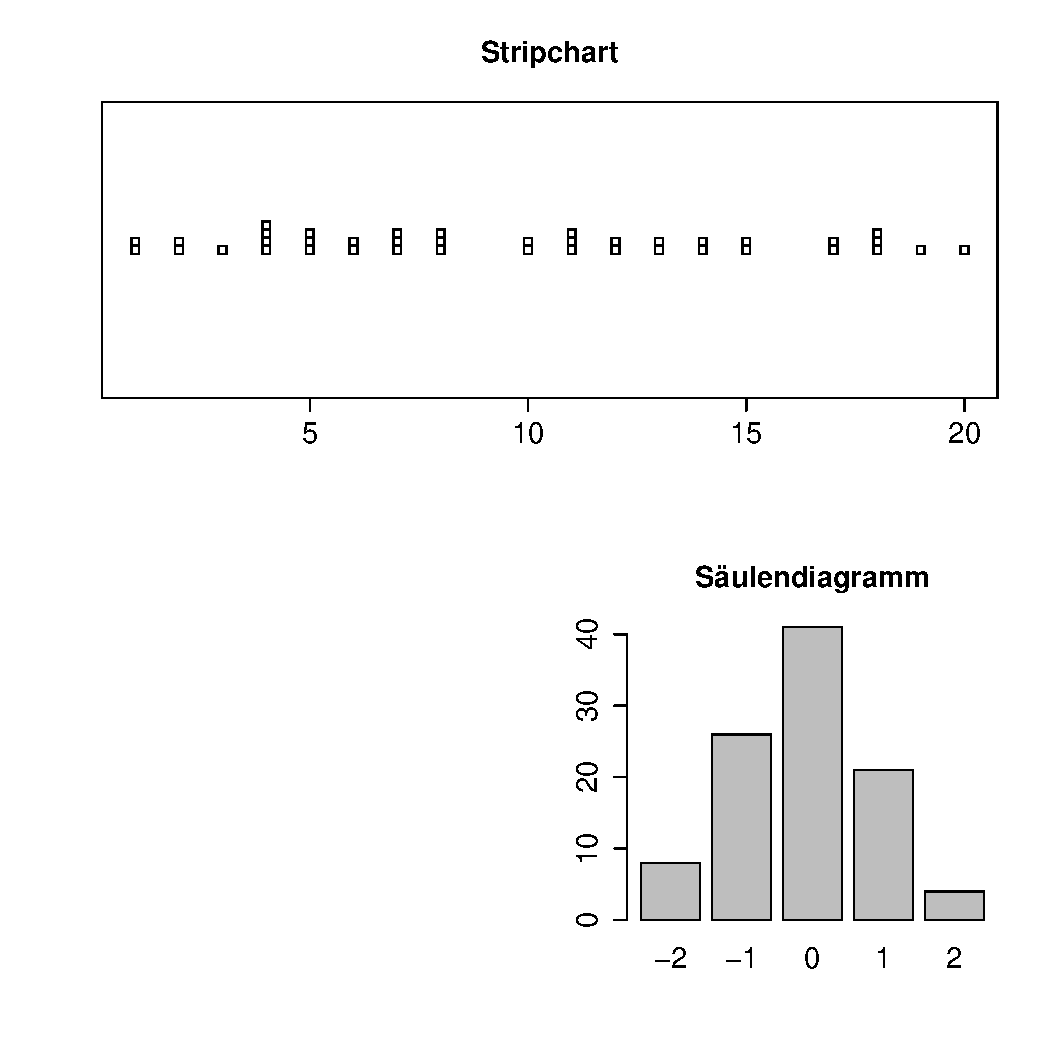
\includegraphics[width=8cm]{layoutComb}
\vspace*{-1em}
\caption{Mehrere, teils zusammengefasste, teils leere Regionen in einem Diagrammfenster mittels \lstinline!layout()!}
\label{fig:layoutComb}
\end{figure}

%%%%%%%%%%%%%%%%%%%%%%%%%%%%%%%%%%%%%%%%%%%%%%%%%%%%%%%%%%%%%%%%%%
%%%%%%%%%%%%%%%%%%%%%%%%%%%%%%%%%%%%%%%%%%%%%%%%%%%%%%%%%%%%%%%%%%
\subsection{\texttt{par(mfrow, mfcol, fig)}}
\label{sec:parMfRow}
%%%%%%%%%%%%%%%%%%%%%%%%%%%%%%%%%%%%%%%%%%%%%%%%%%%%%%%%%%%%%%%%%%
%%%%%%%%%%%%%%%%%%%%%%%%%%%%%%%%%%%%%%%%%%%%%%%%%%%%%%%%%%%%%%%%%%

Ein weiterer Weg Device-Flächen zu unterteilen, besteht in der Verwendung der Argumente \lstinline!mfrow! oder \lstinline!mfcol! von\index[func]{par()@\lstinline{par()}} \lstinline!par()!.
\begin{lstlisting}
par(mfrow=c(<<Anzahl Zeilen>>, <<Anzahl Spalten>>))
par(mfcol=c(<<Anzahl Zeilen>>, <<Anzahl Spalten>>))
\end{lstlisting}

An \lstinline!mfrow! oder \lstinline!mfcol! ist ein Vektor mit zwei Elementen zu übergeben, die die Anzahl der Zeilen und Spalten definieren, aus denen sich dann die einzelnen Regionen der Device-Fläche ergeben. Diese Regionen besitzen dieselbe Größe und lassen sich nicht weiter zusammenfassen. Der Unterschied zwischen beiden Argumenten betrifft die Reihenfolge, in der die entstehenden Regionen mit Diagrammen gefüllt werden: Mit \lstinline!mfrow! werden durch sich anschließende High-Level-Funktionen nacheinander zunächst die Zeilen, bei \lstinline!mfcol! entsprechend nacheinander die Spalten gefüllt. Sind auf der Device-Fläche in einem rechteckigen Layout letztlich \lstinline!<<Anzahl>>! viele Diagramme unterzubringen, kann alternativ auch die Funktion\index[func]{n2mfrow()@\lstinline{n2mfrow()}} \lstinline!n2mfrow(<<Anzahl>>)! zur Erstellung eines geeigneten Vektors verwendet werden, der dann an \lstinline!mfrow! zu übergeben ist.
\begin{lstlisting}
> dev.new(width=7, height=4)                # Diagrammgröße ändern
> par(mfrow=c(1, 2))                        # Diagrammfenster aufteilen
> boxplot(rt(100, 5), xlab=NA, notch=TRUE, main="Boxplot")
> plot(rnorm(10), pch=16, xlab=NA, ylab=NA, main="Streudiagramm")
\end{lstlisting}

Mit \lstinline!par(fig=<<Vektor>>, new=TRUE)! kann alternativ vor einem\index{Grafik!High-Level-Funktion} High-Level-Befehl zum Erstellen eines Diagramms die rechteckige Figure-Region innerhalb der Device-Fläche definiert werden, in die das folgende Diagramm gezeichnet wird.

Die Elemente des Vektors \lstinline!fig! stellen dabei die Koordinaten der Rechteckkanten in der Reihenfolge links, rechts, unten, oben dar und müssen Werte im Bereich von $0$--$1$ besitzen. Der für die untere und obere Kante eingetragene Wert gilt als deren jeweilige $y$-Koordinate, wobei $0$ die Koordinate des unteren und $1$ die des oberen Device-Randes ist. Der für die linke und rechte Kante eingetragene Wert gilt als deren jeweilige $x$-Koordinate, wobei $0$ die Koordinate des linken und $1$ die des rechten Device-Randes ist. Das Argument \lstinline!new=TRUE! legt fest, dass der folgende Grafikbefehl dem aktiven device hinzugefügt werden soll. Indem \lstinline!par(fig)! mehrfach alternierend mit High-Level-Grafikfunktionen aufgerufen wird, lassen sich mehrere Diagramme in einem device plazieren (Abb.\ \ref{fig:parFig}).
\begin{lstlisting}
# Simulation von 1000 mal 10 Bernoulli-Experimenten
> resBinom <- rbinom(1000, size=10, prob=0.3)

# in Faktor umwandeln für mögliche Kategorien, die nicht auftauchen
> facBinom <- factor(resBinom, levels=0:10)

# Häufigkeitsverteilung bestimmen und als senkrechte Linien darstellen
> tabBinom <- table(facBinom)
> par(fig=c(0, 1, 0.10, 1))
> plot(tabBinom, type="h", bty="n", xlim=c(0, 10), xlab=NA,
+      xaxt="n", ylab="Häufigkeit", main="Ergebnisse
+      1000*10 Bernoulli Experimente (p=0.3)")

# Werte zusätzlich als Punkte einzeichnen
> points(names(tabBinom), tabBinom, pch=16, cex=2, col="gray")

# im unteren Diagrammbereich gekerbten Boxplot einzeichnen
> par(fig=c(0, 1, 0, 0.35), bty="n", new=TRUE)
> boxplot(resBinom, horizontal=TRUE, ylim=c(0, 10), notch=TRUE,
+         col="gray", xlab="Anzahl der Erfolge")
\end{lstlisting}

\begin{figure}[ht]
\centering
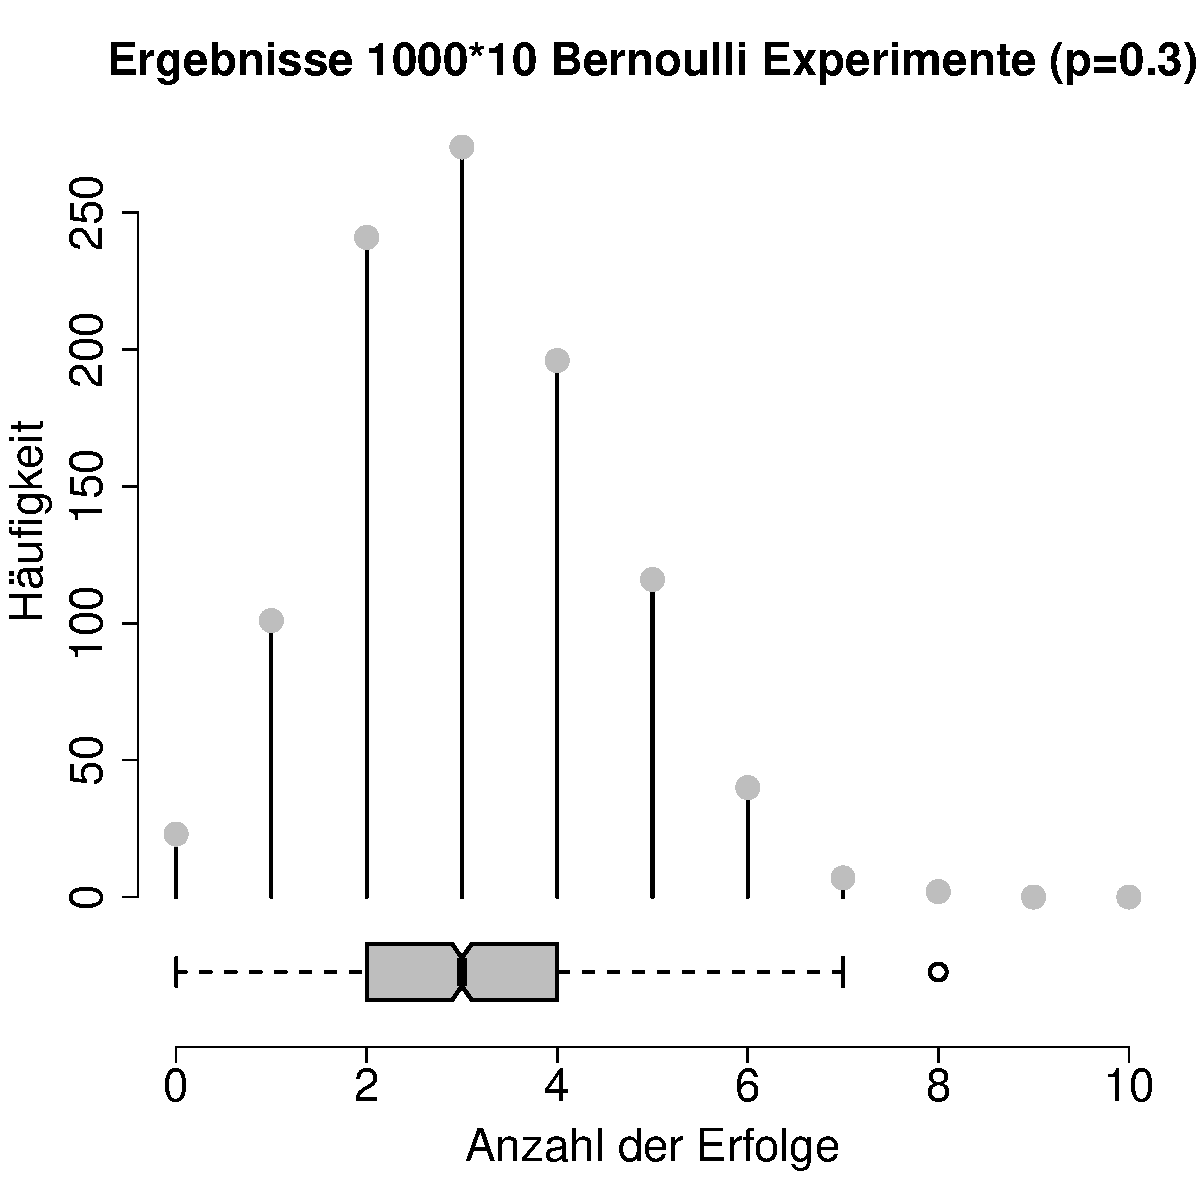
\includegraphics[width=8cm]{parFig}
\vspace*{-1em}
\caption{Anpassen der Größe verschiedener Regionen mit \lstinline!par(fig)!}
\label{fig:parFig}
\end{figure}

%%%%%%%%%%%%%%%%%%%%%%%%%%%%%%%%%%%%%%%%%%%%%%%%%%%%%%%%%%%%%%%%%%
%%%%%%%%%%%%%%%%%%%%%%%%%%%%%%%%%%%%%%%%%%%%%%%%%%%%%%%%%%%%%%%%%%
\subsection{\texttt{split.screen()}}
%%%%%%%%%%%%%%%%%%%%%%%%%%%%%%%%%%%%%%%%%%%%%%%%%%%%%%%%%%%%%%%%%%
%%%%%%%%%%%%%%%%%%%%%%%%%%%%%%%%%%%%%%%%%%%%%%%%%%%%%%%%%%%%%%%%%%

\index[func]{split.screen()@\lstinline{split.screen()}}
Eine dritte Methode, um die Device-Fläche in Regionen zu unterteilen und mit separaten Diagrammen zu füllen, stellt die \lstinline!split.screen()! Funktion bereit, die in Kombination mit \lstinline!screen()! und \lstinline!close.screen()! zu verwenden ist.
\begin{lstlisting}
split.screen(figs=<<2-Vektor oder Nx4-Matrix>>, screen=<<Nummer>>)
\end{lstlisting}

Das Argument \lstinline!figs! erwartet einen Vektor mit zwei Elementen oder eine Matrix mit vier Spalten, die beide die Aufteilung der Device-Fläche definieren können. Ein Vektor legt durch seine beiden Elemente die Zahl der Zeilen und Spalten fest, wie dies auch in \lstinline!par(mfrow)! geschieht. Die Fläche wird in diesem Fall gleichmäßig unter den Regionen aufgeteilt. Dagegen wird jede der in einer für \lstinline!figs! übergebenen vierspaltigen Matrix enthaltenen Zeilen als Definition jeweils einer rechteckigen Region interpretiert. Die Werte in einer Zeile stellen dabei die Koordinaten der Rechteckkanten in der Reihenfolge links, rechts, unten, oben dar und müssen im Bereich von $0$--$1$ liegen. Der für die untere und obere Kante eingetragene Wert gilt als deren jeweilige $y$-Koordinate, wobei $0$ die Koordinate des unteren und $1$ die des oberen Device-Randes ist. Der für die linke und rechte Kante eingetragene Wert gilt als deren jeweilige $x$-Koordinate, wobei $0$ die Koordinate des linken und $1$ die des rechten Device-Randes ist. Auf diese Weise können auch sich überschneidende, oder die Diagrammfläche nicht vollständig ausfüllende Regionen definiert werden (Abb.\ \ref{fig:screen}).

\begin{figure}[ht]
\centering
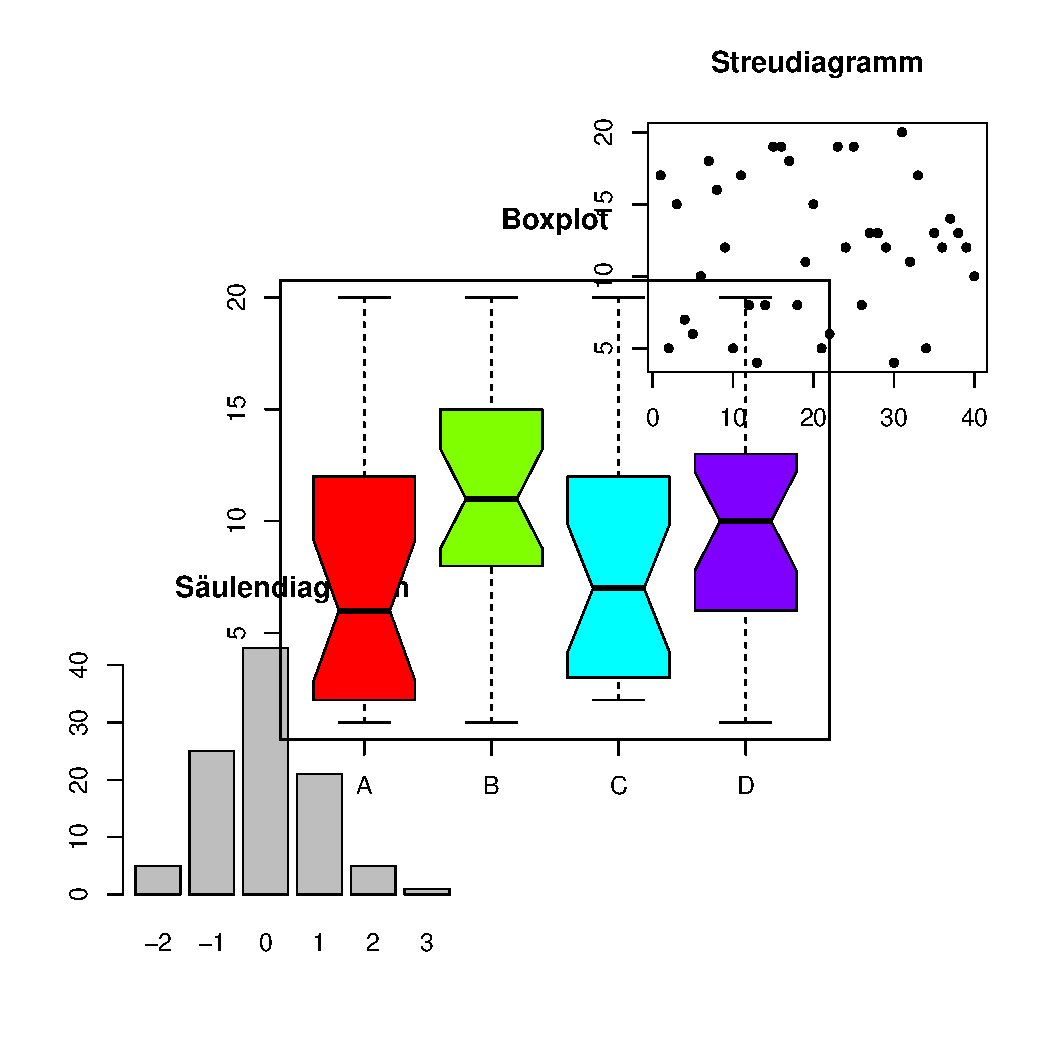
\includegraphics[width=8cm]{screen}
\vspace*{-1em}
\caption{Sich überlappende Regionen mit \lstinline!screen()! erzeugen}
\label{fig:screen}
\end{figure}

Die mit \lstinline!split.screen()! gebildeten Regionen sind intern bei $1$ beginnend numeriert und können über ihre Nummer angesprochen werden. Dies ist in zwei Fällen notwendig: Zum einen kann eine Teilfläche durch erneuten Aufruf von \lstinline!split.screen(screen=<<Nummer>>)! weiter unterteilt werden, wenn dabei an das Argument \lstinline!screen! die Nummer der zu unterteilenden Fläche übergeben wird. Zum anderen muss mit\index[func]{screen()@\lstinline{screen()}} \lstinline!screen(<<Nummer>>)! vor jedem folgenden Befehl zur Diagrammerstellung die Nummer der Fläche genannt werden, in die das Diagramm gezeichnet werden soll.

Eine Teilfläche sollte vollständig bearbeitet werden, ehe die nächste Region ausgewählt wird. Zwar ist es prinzipiell möglich, eine bereits verlassene Teilfläche wieder zu aktivieren, allerdings mit dem Risiko unerwünschter Effekte. Der Inhalt einer mit \lstinline!split.screen()! erzeugten Teilfläche kann mit\index[func]{erase.screen()@\lstinline{erase.screen()}} \lstinline!erase.screen(<<Nummer>>)! wieder gelöscht werden.

Um eine mit \lstinline!split.screen()! erzeugte Teilfläche abzuschließen und damit ein weiteres Hinzufügen von Elementen zu verhindern, dient\index[func]{close.screen()@\lstinline{close.screen()}} \lstinline!close.screen(<<Nummer>>, all.screens=FALSE)!. Mit ihr können über das Argument \lstinline!all.screens=TRUE! auch alle Teilflächen simultan gesperrt werden. Dies sollte etwa geschehen, wenn alle Regionen eines device mit Diagrammen gefüllt und keine weiteren Änderungen gewünscht sind.
\begin{lstlisting}
# 3 Regionen als Zeilen einer Matrix definieren
> splitMat <- rbind(c(0.0, 0.5, 0.0, 0.5), c(0.15, 0.85, 0.15, 0.85),
+                   c(0.5, 1.0, 0.5, 1.0))

> split.screen(splitMat)                   # Diagrammfläche unterteilen
> screen(1)                                # in Region 1 zeichnen
> barplot(table(round(rnorm(100))), main="Säulendiagramm")
> screen(2)                                # in Region 2 zeichnen
> x <- gl(4, 25, labels=LETTERS[1:4])      # Bedingungen
> y <- sample(1:20, 100, replace=TRUE)     # Zielgröße
> boxplot(y ~ x, col=rainbow(4), notch=TRUE, main="Boxplot")
> screen(3)                                # in Region 3 zeichnen
> plot(sample(1:20, 40, replace=TRUE), pch=20, xlab=NA, ylab=NA,
+      main="Streudiagramm")

> close.screen(all.screens=TRUE)           # Bearbeitung abschließen
\end{lstlisting}
